\chapterillustration{./abertura-financeira}{./abertura-financeira-professor}

\expandtocdepth

\bigopenningbox

\chapterwhat{Educação Financeira em Contextos Escolares (EFCE) é um processo de educar a partir de um conjunto de estratégias e ações desenvolvidas para o contexto escolar, considerando aspectos matemáticos e não matemáticos, didáticos e multidisciplinares, que convide os estudantes a refletirem sobre situações econômicas e financeiras relacionadas com a aquisição, planejamento, utilização e redistribuição do dinheiro, de forma crítica e fundamentada. Abordaremos temas como renda e trabalho, planejamento, orçamento e gestão financeira, consumo, cultura e sustentabilidade; o valor do dinheiro no tempo e suas causas: inflação, câmbio, juros e investimentos; equivalência de capitais e de taxas; tributos e contribuições; previdência e proteção, buscando produzir conexões didáticas com a Educação Básica por meio do ensino de matemática, convidando os estudantes a refletirem sobre possíveis consequências de suas decisões e atitudes frente às suas demandas, necessidades, projetos e realizações em sua vida pessoal, familiar e da sociedade em que vivem.}

\chapterbecause{Vivemos diariamente situações financeiras e econômicas que envolvem consumo, poupança, proteção e investimento, em que os nossos desejos, preferências, análises, princípios, valores e escolhas estão presentes e conectadas. Do orçamento financeiro pessoal/familiar aos nossos padrões de consumo; das compras pelos aplicativos às discussões sobre questões demográficas e previdenciárias; das escolhas por produtos sustentáveis ou mais baratos à forma como escolhemos o combustível do automóvel; das nossas decisões sobre onde vamos passar as férias aos planos e estratégias para realizar determinados sonhos, a Educação Financeira aqui abordada será um convite à reflexão sobre situações do dia a dia na busca pelo exercício crítico da cidadania, integrando aspectos matemáticos (em especial da matemática financeira) e não matemáticos (dentre eles os sociais, comportamentais, e ambientais - em especial da psicologia econômica e da sustentabilidade). } 

\chapter{Educação Financeira}
\label{fin-chap}

%%%% Página de Créditos

\autorum{Ivail Muniz Junior}

\revisorum{Amarildo Melchiades da Silva}
\revisordois{Vanessa Matos}

\graficos{Tarso Caldas}

\versao{1.0}

\autordacapa{Josh Appel}{Unsplash}{https://unsplash.com/photos/QSipy5RFcSA}

\creditos

\cleardoublepage
\def\currentcolor{cor1}
\thispagestyle{empty}

\section{Agradecimentos}

Esse capítulo (que mais parece um livro) de Educação Financeira do Livro Aberto é fruto da articulação entre experiência em sala de aula e pesquisa acadêmica. Gostaria de agradecer a alguns interlocutores que foram construindo comigo ao longo de vários anos as ideais que fundamentam essa obra, muito antes dela sequer ser pensada ou concebida, quer como parceiros de pesquisa nos programas de Pós-graduação do Colégio Pedro II, quer em fóruns sobre Educação Financeira no Brasil e fora dele. Agradeço aos professores Daniel Martins, Rony Barros, Josimar Silva e Andreia Maciel do Colégio Pedro II. Aos professores Amarildo Melchiades, Chang Kuo e Marco Kistemann da UFJF; Arthur B. Powell da Rutgers University. Aos professores Carlos Heitor Campani, Marcos Ávila, Vicente Ferreira e da Economista Margarida Gutierrez do Instituto Coppead/UFRJ. Ao professor e contador Luiz Antônio Ochsendorf, da UFRJ e conselheiro do CRC/RJ; aos professores Fernando Villar e Leo Akio do CapUFRJ; Rafael Novoa e André Silva do IFRJ. Às professoras Cristiane Pessoa e Gilda Guimarães da UFPE. A professora Vanessa Matos pela parceria no curso e na finalização deste volume. Aos professores da equipe do Livro Aberto que deram sugestões ao trabalho, em especial a Letícia Rangel, Fábio Simas (Coordenador) e Humberto Bortolossi. Aos meus orientandos Michela Santana, Natasha Cardoso, Vanessa Borges, Wagner Bernardes, Mauricio Quintanilha e Lucas Ribeiro no âmbito dos programas de residência docente, especialização em Educação Matemática e do PROFMAT. A todos os meus alunos da Escola Técnica Estadual João Luiz do Nascimento, do Colégio Pedro II – Campus Centro e do Colégio de São Bento do Rio de Janeiro com os quais tive a honra de conversar, trocar, experimentar e aprender por meio de interações em aulas, bate papos informais, projetos e programas de iniciação científica Júnior. 

Finalmente eu agradeço, em nome da equipe do Livro aberto, aos docentes espalhados pelo Brasil que estiverem efetivamente conosco em nosso primeiro curso de extensão de Educação Financeira no âmbito do Projeto Livro, contribuindo para o aperfeiçoamento desse volume. São eles(elas): Aldair Santana Coelho, Amanda Pereira Lima Mesquita, Ana Clara Bonete, Ana Paula Dantas de Souza, André Monteiro Novaes, Daniela Presotti, Danielle Angélica da Luz e Silva, Dilo Marquesini, Erica Marlucia Leite Pagani, Fábio Henrique da Silva, Fábio Henrique Marinho Cabral, Fábio Pinheiro Pergentino, Fernanda Erculano, Gabriel Bernardino, Jaqueline Cardoni Herrera, José Carlos Nogueira, Josivaldo Gonçalves dos Santos, Ligia Maria Ferreira do Couto, Lucas José Ribeiro, Manoela Franco da Silva, Marciléia Maria da Silva, Nair da Conceição Pinto, Osvaldo Marcelino, Railson Costa da Silva, Raquel Oliveira Bodart, Samuel de Oliveira Cardoso, Sergio Gouveia de Assis, Vanessa Henriques Borges, Virginia Teodoro Inocêncio.

\mainmatter

\begin{apresentacao}{Entendento a ideia do livro: por que Educação Financeira e não Matemática Financeira?}

Gostaríamos de apresentar para você, professor (a), algumas concepções muito importantes para entender esse capítulo de Educação Financeira em Contextos Escolares (EFCE). 

\subsection{Primeira coisa importante}
\begin{center}
\textbf{Tenha em mente que Educação financeira não é Matemática Financeira}
\end{center}
Nossa proposta de Educação Financeira, baseada em Muniz (\citeyear{muniz2016a}, \citeyear{muniz2016b}, \citeyear{muniz2016c}) é um convite à reflexão envolvendo aspectos matemáticos e não matemáticos na reflexão e investigação sobre situações econômico-financeiras (SEF) envolvendo a aquisição, planejamento, uso e distribuição do dinheiro, bem com uma construção de posições fundamentas e críticas sobre atitudes, decisões e suas consequências. 

Olhando para o Brasil, temos vários motivos que justificam a importância de uma Educação Financeira que ajude as pessoas, incluindo nossos alunos, a lidarem com desafios financeiros inseridos em um cenário econômico complexo e dinâmico, como temos observado nas últimas décadas. A estabilidade da moeda (a partir de 1994), o aumento da renda, o crescimento da classe média brasileira, o aumento da oferta de crédito para bens (móveis e imóveis) e serviços, a ampliação do prazo dos financiamentos imobiliários, a velocidade da geração e do consumo de bens e serviços, a redução do grau de desigualdade de renda, além do aumento da expectativa de vida da população, compõem um conjunto de profundadas mudanças sociais e econômicas ocorridas no país que demandam da população brasileira uma educação financeira que traga crítica e atitudes bem fundamentadas. Além dessas mudanças, a crise internacional de 2008 e a recente crise econômica brasileira iniciada em 2015, têm ampliado o conjunto de transformações, trazendo fatores como desemprego, aumento das taxas de inflação e da taxa SELIC, redução do nível de atividade em praticamente todos os setores econômicos, dentre outros. Temos, portanto, uma diversidade de fatores que têm impactado fortemente a vida dos brasileiros, conforme se pode ver em \cite{neri2010}, \cite{PNAD2010}, \cite{leitao2011}.

Nesse texto, entenderemos \textbf{Educação Financeira em Contextos Escolares (EFCE)}, ou simplesmente \textbf{Educação Financeira Escolar}, como o processo de educar por meio de um conjunto de estratégias e ações desenvolvidas para o contexto escolar, considerando aspectos matemáticos e não matemáticos, didáticos e multidisciplinares, que \textbf{convide os estudantes a refletirem} sobre situações econômicas e financeiras relacionadas com a aquisição, planejamento, utilização e redistribuição do dinheiro, de forma crítica e fundamentada, e também sobre possíveis consequências de suas decisões e atitudes frente às suas demandas, necessidades, projetos e realizações em sua vida pessoal, familiar e da sociedade em que vivem.

Um convite que leve em consideração ASPECTOS MATEMÁTICOS E NÃO MATEMÁTICOS na análise e na tomada de decisão, e que também leve em consideração o contexto social e econômico dos estudantes, as características culturais e singularidades sociais da região em que vivem, bem com os desafios da realidade econômica e social brasileira.

Buscamos uma Educação Financeira que estimule os estudantes a pensarem de forma mais crítica e analítica (quando possível), vivendo e se protegendo nessa dinâmica social, aproveitando oportunidades de modo ético e sustentável e se defendendo das muitas armadilhas econômicas e financeiras com as quais certamente têm ou terão que lidar. 

Uma Educação Financeira que leve em consideração as singularidades culturais e sociais da região onde as pessoas vivem, incluindo o poder aquisitivo e seus valores e que os convide a entender que suas escolhas financeiras podem ter impactos não apenas financeiros, mas também políticos, sociais e, também, ambientais. \citep{muniz2016a}.


Assim, nossos objetivos com esse livro aberto é oferecer oportunidades para que estudantes e professores possam ser educados financeiramente, ou seja, que seja, capazes de:

\begin{enumerate}[label=\arabic* --, leftmargin=0pt]
  \item Convidar os estudantes e professores a refletirem sobre situações financeiras e econômicas envolvendo a aquisição, utilização, distribuição e acumulação do dinheiro, por meio da produção de Ambientes de Educação Financeira Escolar.

  \item Convidar os estudantes e professores a refletirem sobre suas atitudes, suas escolhas e as possíveis consequências dessas escolhas, em situações de renda, consumo, risco, poupança e investimento, de modo ético e sustentável. 

  \item Oferecer informações para que sejam aptos a analisar, fazer julgamentos fundamentados, tomar decisões e ter posições críticas sobre questões financeiras que envolvam sua vida pessoal, familiar e da sociedade em que vivem.
\end{enumerate}

\subsection{Segunda coisa importante} 
\begin{center}
\textbf{A Educação Financeira que usamos aqui não é a educação financeira dos Bancos e das instituições financeiras em geral, ainda que usemos vários elementos e ideias dessas abordagens aqui nesse livro.}
\end{center}

Nossa concepção tem várias características diferentes das iniciativas de educação financeira de Bancos, empresas, seguradoras, consultores financeiros, dentre outros agentes. Ela é para a Educação Básica, pensada e testada para produzir Ambientes de Educação Financeira Escolar. 

Essa EFCE que visa mobilizar os estudantes a pensarem de forma crítica (avaliando opções, considerando seus riscos e pensando em possíveis alternativas) se baseia em quatro princípios fundamentais: \textbf{Convite à reflexão, conexão didática, dualidade e lente multidisciplinar}, conforme apresentados em \cite{muniz2016b}.

O \textbf{convite à reflexão} deixa claro que aqui \textbf{não vamos dizer}: seja um poupador; compre sempre à vista; tome crédito para realizar sonhos e ser feliz; torne-se um milionário; seja um empreendedor arrojado; antecipe seu 13$^{\circ}$ ou seu Imposto de Renda, lute ferozmente para ser um vencedor custe o que custar e coisas afins. Não diremos isso, ainda que isso possa ser a escolha de alguns de nossos alunos. A Educação Financeira aqui não será prescritiva ou impositiva, e sim um  \textbf{convite aos estudantes} para que tenham oportunidade de \textbf{reflexão} através da leitura de situações financeiras que contemplem diferentes aspectos, incluindo os de natureza matemática, para que pensem, avaliem e tomem suas próprias decisões. E que essa reflexão inclua mudança de atitude, e os ajude a considerar as possíveis consequências de suas atitudes. Tenha em mente que aquilo que pode ser ótimo para uma pessoa pode ser péssimo para outra, ainda que o ótimo financeiro possa ser um invariante nos dois casos. Então, muito cuidado com os problemas e exercícios: qual é a melhor decisão financeira.

A \textbf{conexão didática} reforça que a EF é na Escola, para a Escola e com a Escola. Esse princípio reforça a importância do contexto escolar no fazer educação financeira. Queremos que essa EFCE ajude a entender como os alunos pensam matematicamente para analisar situações financeiras e que aspectos não matemáticos emergem durante esse processo de ensino e aprendizagem, de modo que essa compreensão gere \textbf{novos materiais, novas formas de ensinar}, e \textbf{novos processos de avaliação}. E que isso contribua para uma melhor formação para o aluno.

A \textbf{dualidade} marca uma posição: a Educação Financeira Escolar pode e deve ser uma via de mão dupla, e portando dual, de modo que tanto os conhecimentos matemáticos dos estudantes os auxiliem na compreensão, análise e tomada de decisão em SEF, como a abordagem de uma EFCE contribua para o desenvolvimento das habilidades matemáticas dos estudantes. Ou seja, ensino de matemática e educação financeira sejam lados de uma mesma moeda.

Finalmente, o princípio da \textbf{lente multidisciplinar} nos traz que é indispensável oferecer múltiplas leituras sobre as situações financeiras, de modo que aspectos financeiros, econômicos, matemáticos, comportamentais, culturais, sociais, políticos e ecológicos possam ser utilizados de forma articulada, na leitura de situações de consumo, renda, endividamento, investimento, planejamento financeiro, sustentabilidade, etc. Estudos do Marketing, da Neurociência, da Economia, da Teoria Cultural do Consumo (Antropologia e Sociologia do Consumo se constituem em diferentes lentes. E como lentes, focam alguns aspectos e desfocam outros.

\begin{figure}[H]
\centering

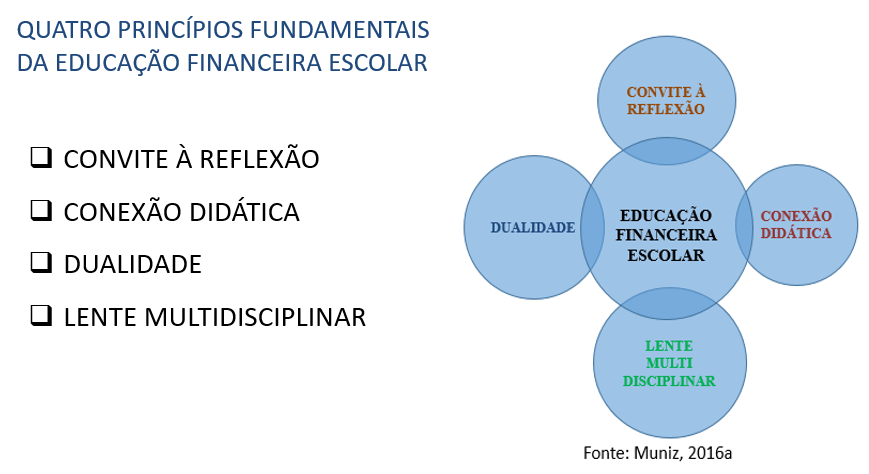
\includegraphics[width=\linewidth]{financeira-professor1}
\end{figure}

\subsection{Terceira coisa importante}

\begin{center}
\textbf{Esse livro não define caminhos, e nem tem a ambição de ser um manual de atividade de educação financiera. O livro aponta princípios e ideias envolvendo aspectos matemáticos e não matemáticos, para que o professor construa, juntamente com seus alunos, seus próprios caminhos, tomem suas próprias decisões e decidam por onde querem ir.}
\end{center}

Há muitas atividades que poderiam ser consideradas como de Educação Financeira, dentre as quais poderíamos citar: a análise de uma conta de luz para identificar excesso de consumo ou possíveis desperdícios; a escolha de um melhor plano de telefonia móvel ou banda larga; uma feira para angariar fundos para uma formatura; uma campanha solidária para arrecadar mantimentos para atender pessoas em tempos de pandemia; o desperdício de comida no refeitório de sua escola; o reaproveitamento de água na escola, e o possível uso dos recursos economizados para a melhoria das condições da quadra esportiva (compra de redes, balizas, ...), dentre outras.

Mas o objetivo desse livro é mostrar alguns princípios e caminhos. Foi mostrar conceitos e ideias. E é claro apresentar algumas atividades para que o professor as utilize como quiser, mas que construa suas próprias atividades, considerando sua realidade econômica, suas peculiaridades regionais, e o perfil de seu aluno, respeitando o direito do estudante de ser quem ele quiser, mas entendendo que suas escolhas e atitudes têm consequências para ele, sua família e para a sociedade em que vivem. 

\textbf{Quarta coisa importante}: para entender a estrutura desse capítulo, olhe o mapa a seguir.

\clearpage

% \hypersetup{linkcolor=\currentcolor}
\end{multicols}
\scexercise{Lista de blocos das seções}
\setlength{\columnsep}{1cm}
\raggedcolumns
\begin{multicols}{2}

\setlist[enumerate]{topsep=0pt}

\scexplore{\hyperref[fin-exp-1]{Explorando 1 --- Em que terreno estamos pisando? O que são situações?}}
\begin{enumerate}[label=Atividade \arabic* --, wide]
\item \hyperref[fin-ativ-1]{Negociando reajustes}
\item \hyperref[fin-ativ-2]{Cobertor curto}
\end{enumerate}

\scarrange{\hyperref[fin-arg-1]{Organizando 1 --- Uma concepção de Educação Financeira para a Escola}}

\scpractice{\hyperref[fin-prac-1]{Praticando 1 --- Ampliando a visão sobre Educação Financeira}}
\begin{enumerate}[label=Atividade \arabic* --, wide]\setcounter{enumi}{2}
\item \hyperref[fin-ativ-3]{Armadilha ou oportunidade}?
\item \hyperref[fin-ativ-4]{O desemprego entre os jovens no Brasil}
\item \hyperref[fin-ativ-5]{A pandemia dos preços}
\end{enumerate}
\vspace{1cm}

\scexplore{\hyperref[fin-exp-2]{Explorando 2 --- Orçamento e Planejamento Financeiros}}
\begin{enumerate}[label=Atividade \arabic* --, wide]\setcounter{enumi}{5}
\item \hyperref[fin-ativ-6]{Como gasto o meu dinheiro?}
\item \hyperref[fin-ativ-7]{Crise à vista: hora de apertar o cinto!}
\end{enumerate}

\scarrange{\hyperref[fin-arg-2]{Organizando 2 --- Diagnóstico e plano de ação na gestão de recursos}}
\begin{enumerate}[label=Atividade \arabic* --, wide]\setcounter{enumi}{7}
\item \hyperref[fin-ativ-8]{O enigma das despesas invisíveis.}
\item \hyperref[fin-ativ-9]{Bola de Neve!}
\end{enumerate}

\scpractice{\hyperref[fin-prac-2]{Praticando 2 --- Ampliando a visão sobre Eduação Financeira}}
\begin{enumerate}[label=Atividade \arabic* --, wide]\setcounter{enumi}{9}
\item \hyperref[fin-ativ-10]{Sonhos de uma bolsista}
\item \hyperref[fin-ativ-11]{Vivendo a vida no slackline}
\end{enumerate}
\vspace{1em}
\columnbreak

\scexplore{\hyperref[fin-exp-3]{Explorando 3 --- O valor do dinheiro no tempo}}
\begin{enumerate}[label=Atividade \arabic* --, wide]\setcounter{enumi}{11}
\item \hyperref[fin-ativ-12]{Iguais podem ser diferentes?}
\item \hyperref[fin-ativ-13]{Inflação: o que eu tenho a ver com isso?}
\item \hyperref[fin-ativ-14]{Passou do vencimento: e agora?}
\end{enumerate}

\scarrange{\hyperref[fin-arg-3]{Organizando 3 --- O valor do dinheiro no tempo: valor presente e valor futuro}}

\scpractice{\hyperref[fin-prac-3]{Praticando 3 --- O valor do dinheiro no tempo: valor presente e valor futuro}}
\begin{enumerate}[label=Atividade \arabic* --, wide]\setcounter{enumi}{14}
\item \hyperref[fin-ativ-15]{O rapaz que editava vídeos.}
\item \hyperref[fin-ativ-16]{O valor do amanhã.}
\item \hyperref[fin-ativ-17]{Tomando decisões diante das emergências.}
\end{enumerate}
\vspace{1em}

\scexplore{\hyperref[fin-exp-4]{Explorando 4 --- O valor do dinheiro no tempo: capitais equivalentes}}
\begin{enumerate}[label=Atividade \arabic* --, wide]\setcounter{enumi}{17}
\item \hyperref[fin-ativ-18]{E o tempo levou!}
\end{enumerate}

\scarrange{\hyperref[fin-arg-4]{Organizando 4 --- O valor do dinheiro no tempo: capitais equivalentes}}

\scpractice{\hyperref[fin-prac-4]{Praticando 4 --- O valor do dinheiro no tempo: capitais equivalentes}}
\begin{enumerate}[label=Atividade \arabic* --, wide]\setcounter{enumi}{18}
\item \hyperref[fin-ativ-19]{Demissão na Pandemia.}
\item \hyperref[fin-ativ-20]{O enigma das taxas de juros invisíveis.}
\end{enumerate}
\vspace{1em}

\scexplore{\hyperref[fin-exp-5]{Explorando 5 --- O valor do dinheiro no tempo: séries uniformes}}
\begin{enumerate}[label=Atividade \arabic* --, wide]\setcounter{enumi}{20}
\item \hyperref[fin-ativ-21]{Disciplina e paciência: nascidas uma para a outra!}
\end{enumerate}

\scarrange{\hyperref[fin-arg-5]{Organizando 5 --- O valor do dinheiro no tempo: séries uniformes}}
\begin{enumerate}[label=Atividade \arabic* --, wide]\setcounter{enumi}{21}
\item[Exemplo 1] \hyperref[fin-exemp-1]{Retomando a atividade inicial}
\item \hyperref[fin-ativ-22]{O dilema de caber no bolso -- parcelas mensais e iguais}
\end{enumerate}

\scpractice{\hyperref[fin-prac-5]{Praticando 5 --- O valor do dinheiro no tempo: séries uniformes e previdência}}
\begin{enumerate}[label=Atividade \arabic* --, wide]\setcounter{enumi}{22}
\item \hyperref[fin-ativ-23]{O que será o amanhã?}
\end{enumerate}
\vspace{1em}

\scexplore{\hyperref[fin-exp-6]{Explorando 6 --- Velozes e furiosas: taxas de juros no cenário brasileiro}}
\begin{enumerate}[label=Atividade \arabic* --, wide]\setcounter{enumi}{23}
\item \hyperref[fin-ativ-24]{Velozes e Furiosas! Uma conversa sobre taxas equivalentes}
\end{enumerate}

\scarrange{\hyperref[fin-arg-6]{Organizando 6 --- Velozes e furiosas: taxas de juros no cenário brasileiro}}

\scpractice{\hyperref[fin-prac-6]{Praticando 6 --- Velozes e furiosas: taxas de juros no cenário brasileiro}}
\begin{enumerate}[label=Atividade \arabic* --, wide]\setcounter{enumi}{24}
\item \hyperref[fin-ativ-25]{Imprevistos e Cheque especial: uma dupla explosiva}
\item \hyperref[fin-ativ-26]{Reduzindo taxas e ampliando oportunidades}
\item \hyperref[fin-ativ-27]{Velozes e Furiosos 2 -- As taxas atacam novamente}
\item \hyperref[fin-ativ-28]{Crédito fácil é caro!}
\end{enumerate}
\vspace{1em}

\scexplore{\hyperref[fin-exp-7]{Explorando 7 --- Inflação e poder de compra}}
\begin{enumerate}[label=Atividade \arabic* --, wide]\setcounter{enumi}{28}
\item \hyperref[fin-ativ-29]{Cadê o meu dinheiro?}
\item \hyperref[fin-ativ-30]{Sua inflação é igual à minha inflação?}
\item \hyperref[fin-ativ-31]{Inflação e Investimentos}
\item \hyperref[fin-ativ-32]{Por que o meu aluguel aumento desse jeito?}
\end{enumerate}
\scarrange{\hyperref[fin-arg-1]{Organizando 7 --- Índices de inflação e seus impactos na vida da população}}

\scpractice{\hyperref[fin-prac-7]{Praticando 7 --- Inflação e poder de compra: dinheiro na mão é...}}
\begin{enumerate}[label=Atividade \arabic* --, wide]\setcounter{enumi}{32}
\item \hyperref[fin-ativ-33]{Inflação e Investimento: impactos nos projetos de longo prazo.}
\item \hyperref[fin-ativ-34]{Qual é a inflação anual no Brasil?}
\end{enumerate}
\vspace{1em}

\columnbreak
\scexplore{\hyperref[fin-exp-8]{Explorando 8 --- Tributação e futuro}}
\begin{enumerate}[label=Atividade \arabic* --, wide]\setcounter{enumi}{34}
\item \hyperref[fin-ativ-35]{Investimento em educação pública no Brasil}
\end{enumerate}
\scarrange{\hyperref[fin-arg-8]{Organizando 8 --- Impostos, taxas e contribuições no Brasil}}

\scpractice{\hyperref[fin-prac-8]{Praticando 8 --- Tributação e investimento}}
\begin{enumerate}[label=Atividade \arabic* --, wide]\setcounter{enumi}{35}
\item \hyperref[fin-ativ-36]{Tributação do IR nos investimentos}
\end{enumerate}

\scexplore{\hyperref[fin-exp-9]{Explorando 9 --- Consumo, cultura, comportamento e sustentabilidade}}
\begin{enumerate}[label=Atividade \arabic* --, wide]\setcounter{enumi}{36}
\item \hyperref[fin-ativ-37]{Liberdade e consumo}
\item \hyperref[fin-ativ-38]{Consumo e Comportamento}
\item \hyperref[fin-ativ-39]{Consumo e proteção de longo prazo}
\end{enumerate}
\scarrange{\hyperref[fin-arg-9]{Organizando 9 --- Consumo e comportamento: herísticas e vieses}}

\scpractice{\hyperref[fin-prac-9]{Praticando 9 --- Comportamento e consumo}}
\begin{enumerate}[label=Atividade \arabic* --, wide]\setcounter{enumi}{39}
\item \hyperref[fin-ativ-40]{Desconto progressivo: oportunidade ou enganação ancorada?}
\item \hyperref[fin-ativ-41]{Indenizações e ancoragem}
\end{enumerate}

\scexercise{\hyperref[fin-exercises]{Exercícios, atividades investigativas e problemas}}
\begin{itemize}
\item Total de 29 atividades
\end{itemize}

\textbf{Total do capítulo = 70 atividades.}

% \relax
% 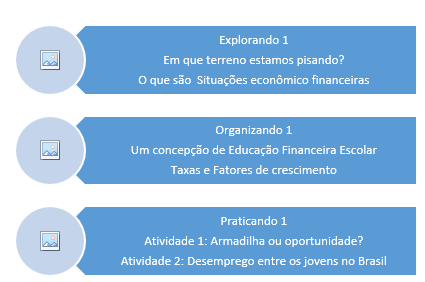
\includegraphics[width=\linewidth]{financeira-professor2}

% 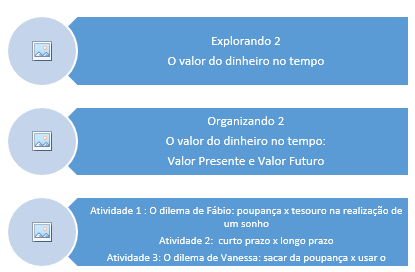
\includegraphics[width=\linewidth]{financeira-professor3}

% 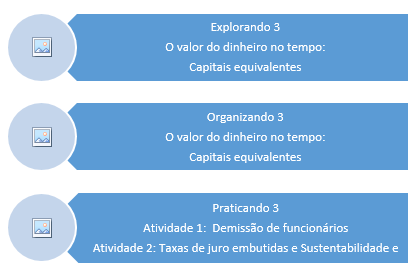
\includegraphics[width=\linewidth]{financeira-professor4}

% 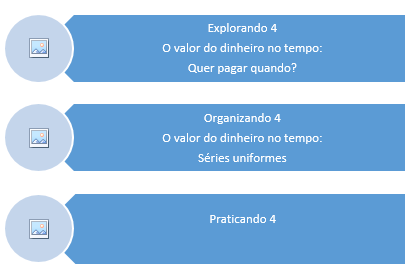
\includegraphics[width=\linewidth]{financeira-professor5}

% 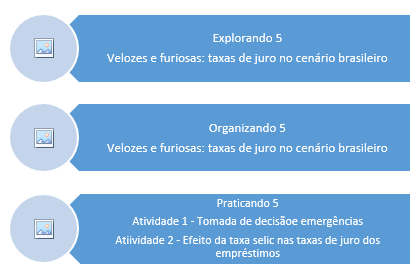
\includegraphics[width=\linewidth]{financeira-professor6}

% 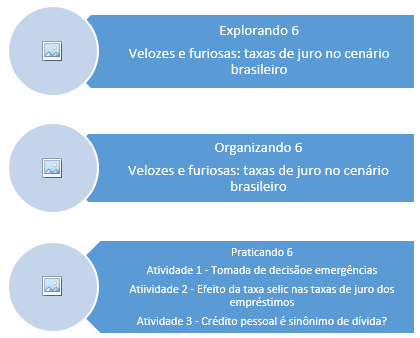
\includegraphics[width=\linewidth]{financeira-professor7}

% 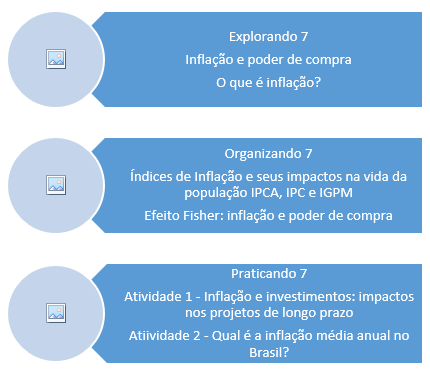
\includegraphics[width=\linewidth]{financeira-professor8}

% 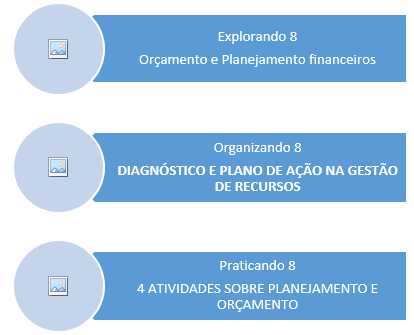
\includegraphics[width=\linewidth]{financeira-professor9}

% 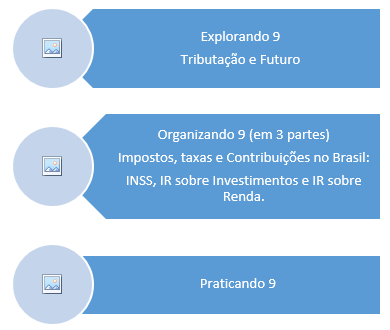
\includegraphics[width=\linewidth]{financeira-professor10}

% 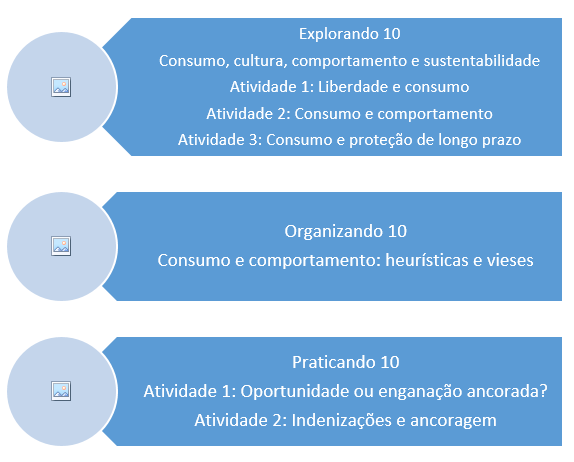
\includegraphics[width=\linewidth]{financeira-professor11}


\end{apresentacao}



\def\currentcolor{session1}
\begin{texto}
{
  \subsection*{Objetivo geral}

  Apresentar os principais objetivos, os temas abordados e a concepção de Educação Financeira que fundamenta todo o capítulo.

  \textbf{Conceitos abordados}: Educação Financeira em contextos escolares (EFCE ou EFE) e Situações Econômico-Financeiras (SEF)

  \begin{habilities}{EM13MAT104}
  Interpretar taxas e índices de natureza socioeconômica, tais como índice de desenvolvimento humano, taxas de inflação, entre outros, investigando os processos de cálculo desses números.
  \end{habilities}

  \subsection{Recomendações para o professor}

  Nessa primeira seção vamos dar um panorama da nossa concepção de Educação Financeira. Basicamente é mostrar que usaremos aspectos matemáticos e não matemáticos, como já explicado antes, para investigar situações, resolver os problemas que forem aparecendo, avaliar cenários possíveis decisões e suas consequências. Temos como objetivo também abordar as noções de taxas de crescimento e fatores de atualização, que são abordados no Ensino Fundamental e em especial no Ensino Médio, tanto em funções como em progressões. 

  Apresentaremos um texto inicial seguido de uma série de situações financeiras que mostram a diversidade de temas relacionados com Educação Financeira que podem ser tratados nas aulas de matemática do Ensino Médio (e alguns deles no Ensino Fundamental também).

  São onze situações que estão associadas às seguintes temáticas:
  \begin{itemize}
  \item Renda e Trabalho
  \item Planejamento, Orçamento e Gestão
  \item Juros: crédito ou investimentos
  \item Consumo, cultura e comportamento
  \item Índices econômicos, câmbio, inflação e poder de compra
  \item Tributação, Contribuições e Futuro
  \item Risco, Retorno e Proteção
  \item Consumo, sustentabilidade e atitude
  \end{itemize}

}
\end{texto}
\clearmargin
\begin{texto}
{
  Essas onze SEF iniciais não são atividades para serem feitas imediatamente. Elas serão exploradas ao longo das seções deste capítulo do Livro Aberto. Algumas delas requerem a construção de conceitos matemáticos mais complexos, como as séries uniformes, por exemplo. Outras até podem ser abordadas imediatamente, conforme a avaliação do professor sobre suas turmas e condições, como as envolvendo planejamento financeiro e comportamento do consumidor. O importante nessa primeira seção é mostrar a diversidade dos temas, sem perder de vista as conexões entre os aspectos matemáticos e não matemáticos existentes nessas SEF.

  Queremos dar um pontapé inicial. É convidar o aluno a perceber a diversidade de situações financeiras que serão tratadas, e como aspectos matemáticos e não matemáticos estarão conectados na análise dessas situações.

  \paragraph{Organização em sala de aula} Peça aos seus alunos para darem exemplos de situações financeiras e econômicas (SEF) que eles já experimentaram. Em seguida, apresente as onze situações financeiras apresentadas nessa seção, tentando ampliar a visão de como tais situações são mais frequentes na vida das pessoas do que eles geralmente pensam, e da importância de se analisar bem para tomar decisões críticas (no sentido de testar a validade, avaliar a viabilidade, e escolher considerando possíveis consequências) e fundamentadas. Convidar os estudantes a pesquisarem informações envolvendo SEF em sites, blogs, jornais, portais, revistas econômicas sobre situações envolvendo inflação, antes de abordar o tema, também pode ampliar o escopo de coisas a partir das quais poderão produzir significados. Convide seus alunos a pesquisarem diferentes estratégias de educação financeira (por exemplo: comparando a do Banco Central com a da sua escola) implementadas em sua região pode ser de bom alvitre. Convide seus alunos a criar a cultura de investigar os fundamentos e a razoabilidade das informações veiculadas nas mídias sociais de forma fundamentada.

  \paragraph{Dificuldades previstas} Esse tema faz um sucesso enorme nas aulas de matemática. Os alunos gostam de conversar sobre SEF pois faz parte da vida deles. Estimule a participação, e procure aproveitar o interesse para trabalhar os conceitos matemáticos. O uso de calculadora pode ajudar, e muito, pois alguns cálculos são simples, mas temos também alguns bem mais complexos. 
}
\end{texto}
\clearmargin
\begin{texto}
{
  \subsection{Sugestões gerais} Lembre-se que você pode abordar os temas de educação financeira (EFE) tais como: planejamento e orçamento financeiro pessoal e familiar, consumo, sustentabilidade, juros, inflação, tributos, previdência, investimentos, dentre outros, por meio de aulas especificas de educação financeira, caso sua escola as ofereça, ou abordar temas a partir dos conceitos e habilidades dentro do teu planejamento nas aulas de matemática. Aborde Educação Financeira para ensinar matemática. Ensine matemática para a reflexão e tomada de decisão em situações financeiras.
}
\end{texto}

\explore{Em que Terreno Estamos Pisando?}
\label{fin-exp-1}
No Brasil, as últimas décadas têm sido de grandes transformações sociais, econômicas, tecnológicas e demográficas. Por exemplo, entre 2002 e 2007, a classe média aumentou de 32\% para 47\% da população total, incorporando mais 23,5 milhões de pessoas. A pobreza extrema passou de 12\% para 5\% no período de 1992 a 2007. Segundo o Instituto de Pesquisa Econômica e Aplicada (IPEA), a desigualdade de renda, medida pelo índice de Gini, foi reduzida de $0{,}604$ para $0{,}556$.

Temos também que a expectativa de vida aumentou de 51 anos em 1950 para quase 73 em 2008. Se os acréscimos na longevidade continuarem nesse ritmo, a expectativa de vida dos Brasileiros será em breve de 81 anos. Da mesma forma, a população com 40 anos ou mais aumentou significativamente ($4,2\%$) em relação a 2006, e houve um decréscimo de $0,7\%$ dos jovens (de 0 a 14 anos) no mesmo período. 

O aumento do crédito cresceu entre 2002 e 2008 de 22\% para quase 40\% do PIB. O controle da inflação e a estabilidade da moeda tem oferecido algumas oportunidades de planejamento financeiro e redução da perda do poder de compra, que não eram possíveis nas décadas de 80 e 90, por exemplo. Além disso, o aumento da oferta de produtos financeiros para financiamentos de veículos, eletrodomésticos, habitação, seguros, previdência, é uma realidade, gerando mais oportunidades e também mais complexidade e responsabilidades nas decisões a serem tomadas.

A educação financeira, em especial a que se volta para a sala de aula de matemática da educação básica, é uma oportunidade de convidar estudantes e professores a refletirem sobre todas essas questões financeiras e econômicas. Nesse texto, pretende-se construir uma educação financeira escolar que seja um convite à reflexão sobre o mundo em que vivemos e construímos, impulsionado por nossas escolhas, atitudes, responsabilidades e compromissos com um futuro sustentável e mais igualitário.

Nesse capítulo vamos abordar algumas situações financeiras e econômicas considerando aspectos matemáticos e não matemáticos na compreensão, análise e tomada de decisão.

\textbf{Para começarmos, convidamos você para uma longa viagem nesse mundo econômico financeiro, onde os aspectos matemáticos e os não matemáticos (comportamentais, sociais, políticos, econômicos e culturais) vão nos acompanhar. Vamos partir das seguintes situações.}

\subsection{Situação 1}
A \textbf{inflação} em um país foi de $8\%$ em 2017 e de $10\%$ em 2018. Os funcionários de uma empresa receberam uma proposta de aumento de $18\%$ para corrigir essas perdas. Você aceitaria essa proposta? Ela realmente corrige as perdas acumuladas nos dois anos? Você apresentaria uma contraproposta, e como argumentaria para defendê-la?


\subsection{Situação 2}
Uma pessoa começa a trabalhar aos 20 anos e pretende se aposentar aos 65 anos. Para ter uma renda \textbf{complementar} de 5 mil reais, por 15 anos (dos 65 aos 80 anos), quanto precisará abrir mão durante todo esse tempo para poder contribuir mensalmente durante os 45 anos, considerando uma taxa média de retorno igual à paga atualmente (2019) pela poupança? E se essa taxa fosse a de um título público pré-fixado? E se fosse a taxa média cobrada pelos quatro principais bancos atualmente instalados no Brasil? 


\subsection{Situação 3}
Quais os motivos na sua opinião que justificam o crescimento apresentado na informação a seguir?


\begin{figure}[H]
\centering
\noindent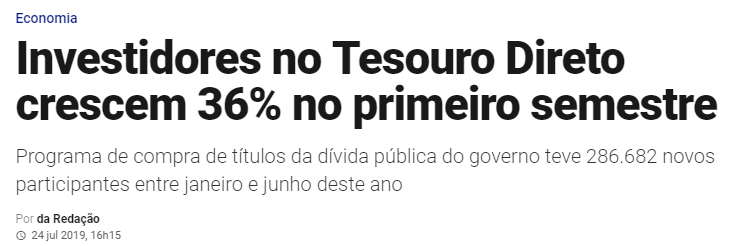
\includegraphics[width=400bp]{tesouro-direto-materia}

\caption{Fonte: \href{https://veja.abril.com.br/economia/investidores-no-tesouro-direto-crescem-36-no-primeiro-semestre/}{Fonte: Revista Veja}. Acesso em 02 de Agosto de 2019.}
\end{figure}



\subsection{Situação 4}
A família Silva identificou que está gastando mais do que ganha, e por dois meses seguidos, seus integrantes gastaram em torno de 400 reais a mais do que ganharam, usando para isso juros do cheque especial com custo de $10\%$ ao mês. Que atitude a família Silva deveria tomar para resolver essa situação? 


\subsection{Situação 5}
Em que aspectos a decisão tomada pelo Banco Central em 31 de julho de 2019 apresentada na informação a seguir influencia a sua vida e de sua família?

\begin{figure}[H]

\centering
\noindent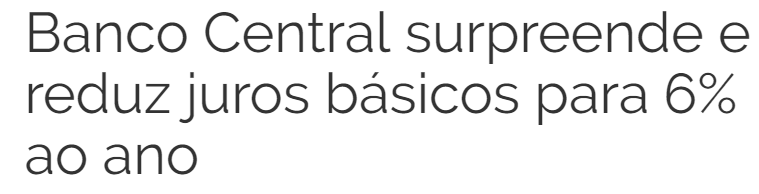
\includegraphics[width=400bp]{bc-juros}

\caption{\href{http://agenciabrasil.ebc.com.br/economia/noticia/2019-07/banco-central-surpreende-e-reduz-juros-basicos-para-6-ao-ano. Acesso em 15 de Agosto de 2019.}{Fonte: Agência Brasil}}
\end{figure}

\subsection{Situação 6}
Você compra um celular por R\$ $1.500{,}00$ reais em dezembro de 2018, e após um ano, ela apresenta um defeito, cujo conserto está estimado em 300 reais. Você também pode trocar seu celular usado por um modelo novo parecido com o seu, pagando 900 reais. Qual decisão você tomaria? Qual o principal aspecto você levaria em consideração para tomar essa decisão? Quais os aspectos matemáticos que você levaria em consideração para tomar essa decisão? Quais aspectos ambientais você costuma levar em consideração para tomar essa decisão?

\subsection{Situação 7}
O Etanol é conhecido por causar menor impacto ambiental que a Gasolina. Entretanto, por questões de eficiência, o Etanol só é vantajoso financeiramente se seu preço corresponder a até $70\%$ do preço da gasolina, como acontece na tabela a seguir:


\begin{itemize}

\item Gasolina: R\$ $4{,}00$/litro 
\item Etanol: R\$ $2{,}80$/litro 

\end{itemize}

Sabendo disso, responda:

\begin{enumerate}
   \item Se o preço do Etanol fosse R\$ $2{,}80$/litro, qual seria sua escolha? E se fosse R\$ $3{,}00$/litro?
   \item Até quanto você estaria disposto a pagar pelo Etanol em prol do meio ambiente?
\end{enumerate}

\subsection{Situação 8}
Você tem dinheiro aplicado na poupança, e pretende comprar um produto com esse dinheiro. Indo a loja, tem duas opções:
\begin{itemize}
\item Comprar à vista com $5\%$ de desconto
\item Ou a prazo, no cartão em 12 vezes sem juros
\end{itemize}

\begin{enumerate}
\item Qual opção você escolheria?
\item Qual a opção mais vantajosa do ponto de vista exclusivamente financeiro? Por que?
\end{enumerate}

\subsection{Situação 9}
A meritocracia tem sido discutida de forma mais intensa ultimamente. Considere as informações apresentadas no gráfico a seguir.

\begin{figure}[H]
\centering

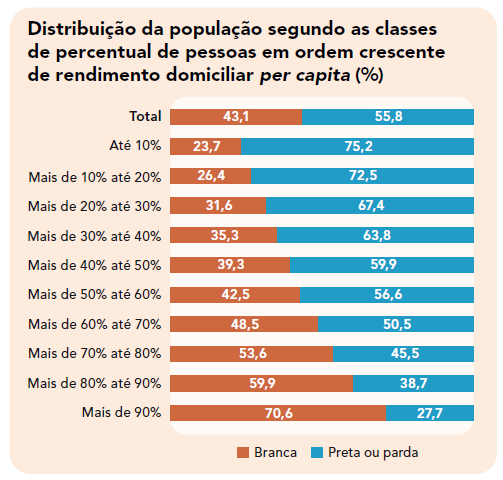
\includegraphics[width=300bp]{financeira1}
\caption{Fonte: \href{https://biblioteca.ibge.gov.br/visualizacao/livros/liv101681_informativo.pdf}{IBGE. Desigualdades por raça e cor no Brasil. Estudos e Pesquisas. Informação Demográfica e Socio Economica. N.41}. Acesso em: 10 set. 2020}
\end{figure}

\begin{enumerate}
  \item Qual a informação que mais lhe chama atenção nesse gráfico?
  \item Como você interpretaria esse gráfico?
  \item Estatisticamente, como você interpretaria a última faixa do gráfico, no contexto da desiguladade salarial em função das questões raciais no Brasil?
\end{enumerate}

\subsection{Situação 10}
\begin{figure}[H]
\centering

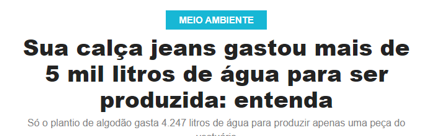
\includegraphics[width=300bp]{financeira2}
\caption{Fonte: \href{https://revistagalileu.globo.com/Ciencia/Meio-Ambiente/noticia/2019/08/sua-calca-jeans-gastou-mais-de-5-mil-litros-de-agua-para-ser-produzida-entenda.html}{Revista Galileu}}

\end{figure}
\begin{enumerate}
  \item Quantas calças jeans você tem em seu guarda roupa?
  \item Qual a relação entre consumo e sustentabilidade na sua família?
\end{enumerate}

\subsection{Situação 11}
Uma família precisa escolher a forma de parcelamento de um bem muito necessário. Após uma pesquisa na internet, o melhor preço à vista, para ser pago no boleto bancário, encontrado foi o seguinte.

\begin{figure}[H]
\centering

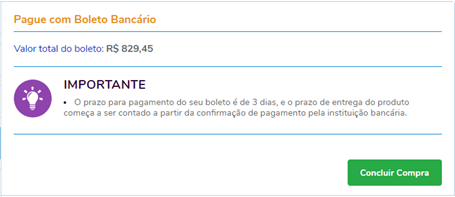
\includegraphics[width=.75\linewidth]{financeira52}
\end{figure}

Como a família não dispõe atualmente de recursos para comprar à vista, ela precisa comprar parcelado. Ela avalia dois tipos de parcelamento disponíveis no site dessa mesma empresa.

\begin{figure}[H]
\centering

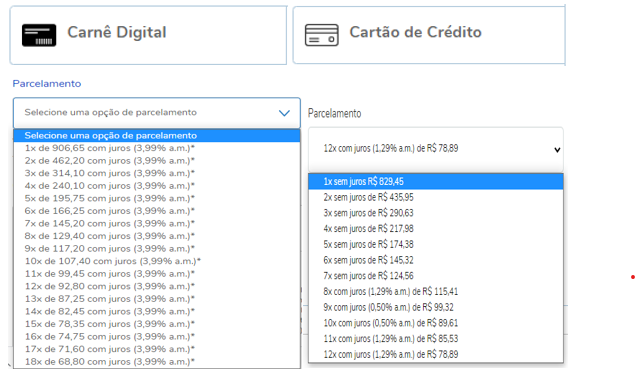
\includegraphics[trim=0 0 2cm 0, clip, width=.7\linewidth]{financeira53}
\end{figure}

\begin{enumerate}
\item Se a família puder pagar uma prestação de até $125$ reais mensais, qual o parcelamento mais econômico?
\item O valor da prestação deve ser o único critério nessa escolha? Justifique.
\item  O que acontece nos dois casos em caso de inadimplência?
\end{enumerate}

Essas situações são apenas algumas das quais iremos abordar ao longo das várias seções deste capítulo de Educação Financeira do Livro Aberto. Observe que temos aspectos matemáticos nelas, mas também temos outros aspectos que não são matemáticos, tais como os financeiros, comportamentais, culturais, econômicos, sociais, políticos, ambientais dentre outros. Nós vamos começar por duas das situações financeiras apresentadas. 

\clearpage
\begin{objectives}{Negociando reajustes}
{
\begin{itemize}
\item Resolver problemas relacionados a percentuais sucessivos e determinação de taxas acumuladas, no contexto da educação financeira.
\item Analisar e tomar decisões em situações econômico-financeiras que envolvam aumentos e/ou descontos sucessivos, considerando aspectos matemáticos e não matemáticos.
\end{itemize}
}{1}{2}
\end{objectives}
\begin{sugestions}{Negociando reajustes}
{
Nessa primeira atividade, convidamos o aluno a pensar sobre os aumentos sucessivos no contexto do reajuste salarial de uma determinada categoria. Os aspectos matemáticos são importantes pois permitem entender que a taxa acumulada não é a soma das taxas, ainda que possa ser obtida por um processo aditivo. Apresentamos dois caminhos para obter a taxa acumulada, sendo o primeiro aditivo (calculando a porcentagem e somando ao valor inicial de cada etapa), e o segundo multiplicativo (considerando a multiplicação pelo fator de atualização $(1+i)$, a cada aumento de uma taxa $i$. Recomendamos sempre que o primeiro processo anteceda o segundo, tanto na abordagem, como para uma possível demonstração. Para alunos do ensino fundamental, o primeiro processo já pode ser abordado aos poucos, conforme inclusive sugere a BNCC com as habilidades \textbf{EF05MA06}, \textbf{EF06MA13}, \textbf{EF07MA02} e \textbf{EF09MA05}. Para os alunos do Ensino Médio, além da retomada das habilidades do ensino fundamental, temos tanto a interpretação situações econômicas (\textbf{EM13MAT101}), como a interpretação e processo de cálculo de taxas e índices de natureza econômica (\textbf{EM13MAT104}), com uma oportunidade para o professor de matemática abordar o conceito de taxa acumulada, a partir de aumentos e descontos sucessivos, em contexto como inflação, salário e renda, bem como discutir as possibilidades de negociação em torno do valor calculado. 
}{0}{0}
\end{sugestions}
\begin{answer}{Negociando reajustes}
{
A solução comentada será apresentada no próprio texto, dentro do tópico Organizando as Ideias.
}{1}
\end{answer}
\begin{objectives}{Cobertor curto}
{
\begin{itemize}
\item Aplicar conceitos matemáticos na construção de orçamentos e planejamentos financeiros (pessoal ou familiar).
\item Analisar e tomar decisões em SEF a partir de orçamentos e planejamentos financeiros, considerando aspectos matemáticos e não matemáticos.
\end{itemize}

}{1}{2}
\end{objectives}
\begin{sugestions}{Cobertor curto}
{
Primeiramente, é importante dizer que teremos sessões específicas para tratar da temática dos juros e do planejamento financeiro. Dois temas importantes para a Educação Financeira das pessoas, em especial, dos nossos estudantes. Entretanto, nessa primeira atividade, já convidamos o aluno a começar a pensar sobre orçamento financeiro (na perspectiva do diagnóstico) e planejamento financeiro (plano de construção e execução ações). A planilha mostra as receitas e despesas (pelo menos as principais) em um quadro de desiquilíbrio. A presença dos juros, que serão abordados detalhadamente na próxima seção, mostra que gastar mais do que ganha tem um custo adicional. E que pagar juros, nessas condições, pode trazer consequências indesejáveis, adiando ou inviabilizando a realização de alguns projetos, sonhos ou expectativas. Reforçamos que teremos uma seção para investigar os diferentes tipos de juros, de forma sistematizada, discutindo por exemplo como podem ser favoráveis ao consumidor, bem como também teremos uma seção para tratar de orçamento e planejamento financeiros de forma detalhada. A presença da porcentagem na atividade aparece como demanda matemática da situação financeira. É no contexto da família que precisa ajustar seu orçamento atualmente desequilibrado que surge a necessidade de se calcular os juros para definir qual a economia necessária no mês seguinte para quitar a dívida e equilibrar o orçamento. Ou seja, os aspectos matemáticos são importantes na construção e execução das ações. 

Essa atividade também está relacionada à habilidade \textbf{EM13MAT203}: aplicar conceitos matemáticos no planejamento, na execução e na análise de ações envolvendo a utilização de aplicativos e a criação de planilhas (para o controle de orçamento familiar, simuladores de cálculos de juros simples e compostos, entre outros), para tomar decisões.
}{0}{0}
\end{sugestions}
\begin{answer}{Cobertor curto}
{
A solução comentada será apresentada no próprio texto, dentro do tópico Organizando as Ideias.
}{1}
\end{answer}
\begin{task}{negociando reajustes}
\label{fin-ativ-1}

A inflação em um país foi de 8\% em 2017 e de 10\% em 2018. Os funcionários de uma empresa receberam uma proposta de aumento de 18\% para corrigir essas perdas. Ela realmente corrige as perdas acumuladas pela inflação nos dois anos? Você aceitaria essa proposta? Se você não aceitasse essa proposta, qual a contraproposta que você apresentaria, e como argumentaria para defendê-la?
\end{task}

\begin{task}{cobertor curto}
\label{fin-ativ-2}

A família Silva identificou que está gastando mais do que ganha, e para isso está usando o cheque especial, que custa 10\% ao mês, sobre o saldo devedor. O orçamento doméstico simplificado da família em Janeiro e fevereiro desse ano estão representados na tabela a seguir.

\begin{table}[H]
\centering
\begin{tabular}{|c|c|c|c|}
\hline
\tmcol{2}{|c|}{Receitas} & \tmcol{2}{|c|}{Despesas}\\
\hline
\tcolor{Descrição} & \tcolor{Valor (R\$)} & \tcolor{Descrição} & \tcolor{Valor (R\$)}\\
Salário Pai & 1.800{,}00 & Alimentação & 1.100{,}00 \\
\hline
Salário Mãe & 2.200{,}00 & Luz & 180{,}00 \\
\hline
& & Água & 80{,}00\\
\hline
& & Telefone & 450{,}00 \\
\hline
& & Aluguel & 1.200{,}00 \\
\hline
& & Cartão de Crédito & 750{,}00 \\
\hline
& & Lazer &300{,}00\\
\hline
& & Transporte & 440{,}00\\
\hline
\tcolor{Total} & \tcolor{4.000{,}00} & \tcolor{Total} & \tcolor{4.500{,}00}\\
\hline

\end{tabular}
\end{table}

\begin{enumerate}

\item Considerando que eles fiquem devendo os R\$ $500{,}00$ durante 15 dias ao Banco, ou seja, peguem R\$ $500{,}00$ emprestado usando o crédito do cheque especial por 15 dias, quantos reais, aproximadamente, eles terão que economizar no mês seguinte para equilibrar o orçamento?

\item Quais seriam as sugestões que você daria para ajudar a família Silva a resolver esse problema no orçamento? 
\end{enumerate}

\end{task}


\arrange{Uma Concepção de Educação Financeira}
\label{fin-arg-1}

Observe que na primeira atividade, somos inclinados a pensar que a inflação acumulada nos dois anos é a soma das inflações em cada ano. A ideia mais simples e usual é recorrer ao processo aditivo. Nosso cérebro adora atalhos e gosta de dar respostas rápidas a problemas numéricos \citep{kahneman2012}. Nesse caso, esse atalho nos leva a um engano, podendo ter como consequência aceitar um reajuste que não repõe a inflação acumulada, ou seja, que não mantém o poder de compra desse salário. Assim, não compreender os aspectos matemáticos dessa situação pode levar a uma redução do poder de compra de uma família. Quantas pessoas você conhece que realmente acham que os 18\% de reajuste corrigiriam a inflação acumulada nos dois anos? Mas, por que não corrige?

Consideremos um produto que custava 100 reais no início no final de 2017, e que aumente exatamente conforme a inflação apresentada. O que acontece com esse preço após os dois aumentos sucessivos? Vamos usar uma representação, que chamaremos de representação temporal, para nos ajudar a entender o a transformação do preço nesses dois anos.  

\begin{figure}[H]
\centering

\begin{tikzpicture}[node distance = 3.5cm, ->]

\node (A) {100{,}00};
\node (B) [right of=A] {108{,}00};
\node (C) [right of=B] {118,80};

\path
(A) edge [color=\currentcolor, very thick] node [above, black] {2017} node [black,below]  {8\%} (B)

(B) edge [color=\currentcolor, very thick] node [above, black] {2018} node [black,below] {10\%} (C);
\end{tikzpicture}

\end{figure}

Essa representação apenas registra que o produto que custava R\$ $100{,}00$, no início de 2017, passou a custar um ano depois: $100{,}00 + 8\%\times100{,}00 =$ R\$ $108{,}00$. E que esses R\$ $108{,}00$, do início de 2018 passarão a custar $108{,}00 + 10\% \times 108{,}00 = \text{R\$ } 118{,}80$ no final de 2018. 

Logo o preço passou de $100$ para $118{,}80$, o que resulta em uma variação de $18{,}80\%$. Assim, um reajuste de $18\%$ não corrige as perdas pela inflação, ou seja, um reajuste de $18\%$ não vai ser suficiente para que se compre a mesma quantidade de produtos, supondo que aumentassem os $18{,}80$\% de inflação no período. Nesse caso, teríamos uma redução do poder de compra. Para manter o poder de compra, tomando como base a inflação, os salários deveriam ser reajustados em $18{,}8\%$, e não em 18\% como muitos poderiam pensar. 

Para analisar essa situação, também poderíamos pensar assim: 

\begin{center}
\textbf{Uma quantia, ao ser aumentada de uma taxa $i$, fica multiplicada por $1+i$}
\end{center}

Usando essa ideia, o preço fica multiplicado por $1{,}08$ quando aumenta de $8\%,$ e em seguida por $1{,}10$ quando aumenta $10\%$, sendo, portanto multiplicado por $1{,}10\times1{,}08 = 1{,}188$. Logo o aumento foi de $18{,}8\%$ em dois anos.

De uma maneira geral, uma quantia $C$, ao variar de uma taxa $i$, transforma-se em:

$$ C+iC=C\cdot(1+i) $$


De um modo geral, esse fator é chamado de fator de atualização. Observe que esse fator atualiza, nesse contexto, os preços anuais.

Há uma questão financeira relevante aqui. Observe que o valor dos preços, diante de uma inflação diferente de zero, se transforma no tempo. De fato, a inflação é um dos fatores que modificam o valor de uma quantia no tempo, assim como o câmbio, os juros, a demanda, a geração de valor por meio de investimentos, dentre outros.

Mas há outros aspectos importantes que podem ser levados em consideração nessa situação, além dos aspectos matemáticos tratados até aqui. As condições econômicas tais como desemprego, queda nas vendas, condições climáticas, dentre outras podem afetar essa negociação, gerando acordos entre patrões e empregados abaixo dos $18{,}8\%$, que seria o mínimo necessário para manter o poder de compra considerando essa inflação acumulada.

Outro aspecto é que um índice de inflação sempre considera um conjunto particular de produtos e serviços, alguns dos quais podem não fazer parte da realidade de uma pessoa ou não ter o mesmo peso. Qual é a sua inflação, baseado no teu perfil de consumo? Esse reajuste calculado baseado nessa inflação acumulada corrigiria a tua inflação? Voltaremos a discutir essa temática de forma mais detalhada numa seção mais adiante.

Entenda que todas essas questões já apontam para uma natureza bem especial das situações econômico-financeiras que abordaremos nesse capítulo: os aspectos matemáticos estarão conectados aos aspectos não matemáticos para nos ajudar a investigar, refletir e tomar decisões. 

Na educação financeira presente nesse livro, queremos olhar para cada situação por diversos pontos de vista, buscando sempre usar a matemática articulada com outras áreas do conhecimento para ampliar nossa compreensão daquilo que estamos analisando.

Já na \textbf{segunda atividade}, é muito comum pensar que a economia a ser realizada no mês seguinte é de $500$ reais. Ou ainda, que a economia para o mês seguinte é de apenas $25$ reais (um valor aproximado para os juros que serão pagos). 


Qual a economia a ser realizada no mês seguinte ao apresentado? Qual o valor máximo que eles podem gastar para equilibrar o orçamento a família no mês seguinte? 

A resposta é de aproximadamente R\$ $1.025$. Isso mesmo! Pois eles precisam economizar os $500$ reais do mês anterior mais os $500$ reais do mês em questão, pois o orçamento está desequilibrado em $500$ reais, e ainda pagar os juros de $25$ reais. Ou seja, ao invés de terem os 4000 reais a disposição, terão apenas $4.000{,}00 - 1.025{,}00 = 2.975{,}00$ reais. Um preço que se paga por gastar mais do que se ganha.

Isso vai demandar um esforço dos integrantes da família, exigindo sacrifícios durante algum tempo. Essa família precisará redefinir prioridades, estabelecer metas claras, mudar comportamentos, e ter uma atitude que costuma ser considerada bem desafiadora: manter a disciplina para cumprir o que foi planejado. Além dos aspectos matemáticos, nos quais a família precisa se apoiar para equilibrar o orçamento, há aspectos comportamentais que estarão presentes nesse processo.

Essa articulação entre diferentes aspectos é uma das características do que vamos chamar de Educação Financeira. \textbf{Mas o que é Educação Financeira?}

A definição que mais tem sido usada no Brasil é a da Organização para Cooperação e Desenvolvimento Econômico (OCDE), apresentada em 2005, que diz que Educação Financeira é o processo pelo qual as pessoas melhoram seus conhecimentos financeiros, sua compreensão do mercado e seu nível de informação sobre produtos e serviços de consumo, crédito, investimento, seguros, previdência dentre outros, evitando armadilhas e sabendo como e quando procurar ajuda, que lhes permitem planejar e fazer escolhas de curto, médio e longo prazo que visem e efetivamente produzam o seu bem estar e de sua família.

Mas será que essa definição contempla todas as dimensões que precisamos para sermos educados financeiramente? Entendemos que não! Há outras questões que precisam ser levadas em consideração na visão sobre como lidamos com o nosso consumo, aquisição, utilização, poupança e distribuição do dinheiro? Vamos mostrar que sim!

Nesse texto, usaremos uma outra concepção de Educação Financeira, mais adequada aos propósitos do livro aberto, que passaremos a chamar de \textbf{Educação Financeira em Contextos Escolares}.

A partir de agora, vamos então chamar de \textbf{Educação Financeira em Contextos Escolares (EFCE)} ao processo de educar a partir de um conjunto de estratégias e ações desenvolvidas para o contexto escolar, considerando aspectos matemáticos e não matemáticos, didáticos e multidisciplinares, que \textbf{convide os estudantes} a refletirem sobre situações econômicas e financeiras relacionadas com a aquisição, planejamento, utilização e redistribuição do dinheiro, de forma crítica e fundamentada, e também sobre possíveis \textbf{consequências de suas decisões e atitudes} frente às suas demandas, necessidades, projetos e realizações em sua vida pessoal, familiar e da sociedade em que vivem.

Abordaremos temas como renda e trabalho, planejamento, orçamento e gestão financeira, consumo, cultura e sustentabilidade; o valor do dinheiro no tempo e suas causas: inflação, câmbio, juros e investimentos; equivalência de capitais e de taxas; tributos e contribuições; previdência e proteção, buscando produzir conexões didáticas com a Educação Básica por meio do ensino de matemática, convidando os estudantes a refletirem sobre possíveis consequências de suas decisões e atitudes frente às suas demandas, necessidades, projetos e realizações em sua vida pessoal, familiar e da sociedade em que vivem.

Com esse livro, queremos contribuir para que você seja educado financeiramente, isto é, que seja capaz de:

\begin{enumerate}[label=\arabic*.]

\item Refletir sobre situações financeiras e econômicas envolvendo a aquisição, utilização, distribuição e acumulação do dinheiro, por meio da produção de Ambeintes de Educação Financeira Escolar.

\item Refletir sobre suas atitudes, suas escolhas e as possíveis consequências dessas escolhas, em situações de renda, consumo, risco, poupança e investimento, de modo ético e sustentável. 

\item Investigar, analisar, fazer julgamentos fundamentados, tomar decisões e ter posições críticas sobre questões financeiras que envolvam sua vida pessoal, familiar e da sociedade em que vive.

\end{enumerate}

\begin{knowledge}

A palavra "economia"{} foi cunhada pelo filósofo Xenofante na Grécia Antiga. Combinando oikos, que significa "casa de família"{}, "agregado familiar"{}, com nomos, que significa regras ou normas, ele inventou a arte de gerir um lar, e isso não poderia ser mais relevante nos dias de hoje. Economia tem a ver com a gestão de recursos individuais e coletivos, incluindo o planeta, uma vez que a atividade humana, está colocando uma pressão sem precedentes sobre os sistemas geradores de vida na Terra.

\vspace{1em}
Kate Raworth - Professora e Pesquisadora da Universidade de Oxford.

\textit{Fonte: Economia Donut. Uma alternativa ao crescimento a qualquer custo. Rio de Janeiro: Zahar. 2019}

\end{knowledge}

\clearpage
\def\currentcolor{session2}
\begin{objectives}{Armadilha ou oportunidade?}
{
\begin{itemize}
\item Resolver problemas relacionados a aumentos e/ou descontos no contexto da educação financeira.
\item Analisar e tomar decisões em situações econômico-financeiras que envolvam aumentos e/ou descontos, considerando aspectos matemáticos e não matemáticos.
\end{itemize}
}{1}{2}
\end{objectives}
\begin{sugestions}{Armadilha ou oportunidade?}
{
Nessa atividade buscamos apresentar uma situação de consumo que convida o estudante a refletir sobre estratégias de venda, baseada em aumento (implícito) seguido de desconto (potencialmente ilusório), muitas vezes com o intuito de produzir no cliente uma possível sensação de ganho na compra de um produto. Para isso colocamos duas situações cujos preços são iguais, mas que podem mobilizar reações comportamentais diferentes, onde a sensação de ganho na segunda situação é fortemente estimulada, quando na comparação com a primeira. \citep{kahneman2012}.

Aqui também buscamos, intencionalmente, usar a lente da Psicologia Econômica para introduzir a noção de ancoragem e de como esse efeito tem sido usado para influenciar as pessoas. 

O processo mental de usar valores como referências de modo consciente ou inconsciente para tomar decisões é chamado de Ancoragem, conforme os estudos da psicologia econômica, dentre eles os de \citeauthor{kahneman2012} e Tversky (\citeyear{kahneman2012}).

Olhando para a atividade, é importante ter em mente os 500 reais podem estar ali porque a bolsa realmente custava $500$ reais, ou como armadilha mental, ou seja, apenas para servir de referência de modo a induzir nossa mente a acreditar na sensação de ganho, de oportunidade. 
Discuta com seus alunos essas duas possibilidades, mostrando a eles que muitas estratégias comerciais usam âncoras, valores que tomamos como referência para tomar decisões, e que tais valores podem ser usados intencionalmente para se pagar mais caro por um produto. Colocar um produto bem mais caro ao lado de um mais barato para criar a sensação de ganho, ainda que o mais barato esteja mais caro do que em outros lugares; usar preços como $2{,}99$ e não $3{,}00$ reais; quebrar a proporcionalidade na venda de produtos, para induzir maio consumo como no caso da pipoca no cinema, do milk shake nas lanchonetes famosas de fast food; inserção de produtos super caros em cardápios para induzir a compra de produtos caros de menor preço são apenas alguns exemplos em que ancoragem é usada para induzir comportamento. 

Recomendamos ao professor que peça aos alunos para pesquisarem na internet matérias, vídeos, e informações sobre a Black Friday, onde algumas práticas enganosas usando a estratégia de dar descontos sobre preços previamente aumentados, geraram um dos memes mais famosos sobre esse período: a Black Fraude. 

}{0}{1}
\end{sugestions}
\begin{answer}{Armadilha ou oportunidade?}
{
\begin{enumerate}
\item A loja que atrairia mais compradores poderia ser a loja b, pois o consumidor poderia ser levado a pensar que estivesse tendo vantagem por conta do desconto de mais da metade do valor da bolsa. A sensação de ganho geralmente costuma atrair as pessoas. Então a loja B tende a atrair mais compradores. 

\item A segunda pergunta é pessoal, sendo muito importante deixar os alunos falarem. Resposta individual.

\end{enumerate}
}{1}
\end{answer}

\begin{knowledge}
Apesar das iniciativas nos EUA com o \textit{National Endowment for Financial Education}/NEFE, na década de 80, e o \textit{JumpStart Coalition for Personal Financial Literacy}, na década de 90, poderem ser consideradas os movimentos precursores das ações de Educação Financeira em grande escala, foi a OCDE em 2003, dois anos após a queda das torres do World Trade Center e seus profundos desdobramentos políticos e econômicos no mundo, quem produziu o primeiro grande estudo sobre EF em nível Internacional, intitulado \textit{Melhoria da literacia financeira: análise das questões e políticas}, do qual veio o documento \textit{Recomendações sobre os princípios e boas práticas para a Educação Financeira e consciência}, que passou a ser referência mundial, presente em vários programas e documentos que fundamentam as iniciativas de Educação Financeira dos países que optaram por seguir tais recomendações, conforme apontam \cite{silva2013} e \cite{muniz2016b}.
\end{knowledge}

\clearmargin
\begin{objectives}{O desemprego entre os jovens no Brasil}
{
\begin{itemize}
\item Interpretar criticamente situações econômicas, sociais que envolvam aumentos e/ou descontos percentuais, considerando aspectos matemáticos e não matemáticos.
\item  Resolver problemas relacionados a aumentos e/ou descontos percentuais no contexto da educação financeira.
\end{itemize}
}{1}{1}
\end{objectives}
\begin{sugestions}{O desemprego entre os jovens no Brasil}
{
Nessa atividade abordamos a temática Renda e Trabalho para convidar o estudante a refletir sobre a situação do jovem brasileiro que precisa ou opta por trabalhar, em uma fase da vida onde a formação inicial está (ou deveria estar) em curso. Aproveitamos para abordar a diferença entre aumentos percentuais e pontos percentuais, por se tratar de dois conceitos muito parecidos, mas essencialmente diferentes, e que costumam causar grande confusão. Quando algo aumenta de $20\%$ para $30\%$, é muito comum pensar que o aumento foi de $10\%$, quando na verdade tivemos um aumento de $10$ pontos percentuais, o que representa um aumento de $50\%$. 

Recomendamos que o professor de matemática, em parceria com o de Geografia ou Sociologia por exemplo, discuta a partir das informações apresentadas na matéria, das fontes citadas no texto, de outras fontes contendo dados estatísticos de órgãos oficiais, algumas questões, dentre elas: 

\begin{itemize}
\item Por que a situação brasileira afeta mais os jovens?
\item Por que as taxas de desemprego entre os jovens no Brasil são tão altas, comparadas ao norte da África e ao Oriente Médio?
\item Qual o perfil do jovem que não estuda e nem trabalha?
\item O que poderia ser feito para mitigar o problema? 
\end{itemize}

Essa atividade também está relacionada à habilidade \textbf{EM13MAT101}: Interpretar criticamente situações econômicas, sociais e fatos relativos às Ciências da Natureza que envolvam a variação de grandezas pela análise das taxas de variação. 
}{1}{1}
\end{sugestions}
\begin{answer}{O desemprego entre os jovens no Brasil}
{
\begin{enumerate}
\item O título da matéria aponta para o problema social do desemprego. O principal problema é a situação do setor da economia brasileira que afeta no desemprego quando não está boa.
\item  O aumento em pontos percentuais da taxa de 2013 para 2019 foi de $12{,}1\%$. E o aumento percentual da taxa de 2013 para 2019 foi de aproximadamente $77{,}07\%$.
\item No ano de 2020 os jovens ainda enfrentam o problema social do desemprego como no ano de 2018. Então a imagem ainda continua atual e representa de fato o problema social da matéria.  

\end{enumerate}
}{0}
\end{answer}
\begin{objectives}{A pandemia dos preços}
{
\begin{itemize}
\item Interpretar criticamente situações econômicas, sociais que envolvam aumentos e/ou descontos percentuais, considerando aspectos matemáticos e não matemáticos.
\item Resolver problemas relacionados a aumentos e/ou descontos percentuais, incluindo os sucessivos, no contexto da educação financeira.
\end{itemize}
}{1}{2}
\end{objectives}
\begin{sugestions}{A pandemia dos preços}
{
Nessa atividade abordamos a temática aumento de preços, em especial a ocorrida com os alimentos na Pandemia de 2020. 

Além dos aumentos percentuais, convidamos o aluno a pensar em questões econômicas como oferta e demanda, variação cambial, políticas de estoque dentre outras. 

Essa atividade também está relacionada à habilidade \textbf{EM13MAT101}: Interpretar criticamente situações econômicas, sociais e fatos relativos às Ciências da Natureza que envolvam a variação de grandezas pela análise das taxas de variação. 

}{1}{2}
\end{sugestions}
\begin{answer}{A pandemia dos preços}
{
\begin{enumerate}
\item Resposta pessoa. Para famílias de menor poder aquisitivo espera-se que o impacto tenha sido maior, principalmente com o aumento de consumo com mais pessoas ficando em casa.
\item De 15 para 40 a variação percentual foi de $40/15-1=166{,}7\%$
\item 
Há várias razões. Aqui sugerimos uma parceria com o professor de Geografia. Mas o mais recomendado é uma boa pesquisa em matérias nos principais jornais do país, pela internet. Há uma grande conjugação de fatores que contribuiu, em especial, para o aumento de preço dos alimentos, segundo os especialistas. Em especial, o preço do arroz tem sido influenciado por:

\begin{itemize}
\item Alguns dos principais exportadores mundiais de arroz, restringiram suas exportações. Se a oferta mundial diminui, o preço tende a aumentar, modificando o ponto de equilíbrio. 

\item Pandemia. Influencia na medida que alterou o consumo desse tipo de item nas famílias. Mais pessoas comendo em casa, e comendo mais, gera maior demanda por alguns tipos de alimentos. E demanda altera o ponto de equilíbrio. 

\item Desvalorização do real frente ao dólar. Com isso o preço aumenta, aumentando o custo de quem vende para o consumidor final. 

\item Produtores do Brasil, diante do preço maior lá fora, preferem vender mais caro para fora. Logo o preço aqui vai subir. (Matéria hoje na Folha de SP mostra isso, com depoimentos dos próprios produtores).

\item Redução do número de produtores de arroz no Brasil, em função de um retorno mais baixo, nos últimos anos, quando comparado a outros alimentos. Influencia na oferta. (Matéria hoje na Folha de SP mostra isso).

\item Redução do papel da CONAB na regulação dos estoques de forma intencional pelo atual governo.
\end{itemize}
\clearpage
\item $P=40\times(1-5\%)\times(1-5\%)=40\times0{,}95^2=36{,}10$. Logo, o preço após duas semanas, nessas condições, seria de R\$ $36{,}10$.
\item É possível obter uma estimativa do tempo mínimo para o preço voltar aos $15$ reais modelando o problema por meio de uma função exponencial, recaindo em uma equação exponencial, que para ser resolvida demandaria usualmente os logaritmos, conforme a modelagem matemática a seguir:

\begin{align*}
40\cdot0{,}95^t&=15\\
0{,}95^t&=\frac{15}{40}\\
t&=\frac{\log15-\log40}{\log95-\log100}\\
t&\cong19{,}12\text{ semanas}
\end{align*}

\end{enumerate}
}{9}
\end{answer}

\practice{Ampliando a Visão Sobre EF}
\label{fin-prac-1}

\begin{task}{Armadilha ou oportunidade?}
\label{fin-ativ-3}
Observe a seguinte bolsa sendo divulgada em duas lojas diferentes:

\begin{figure}[H]
\centering

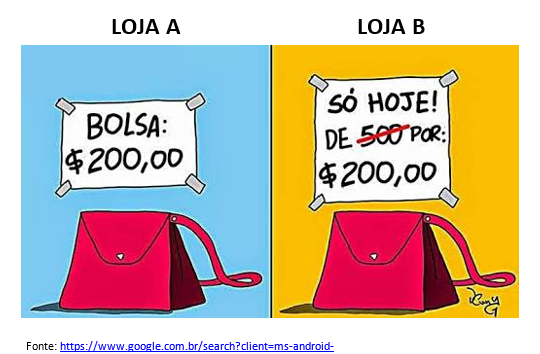
\includegraphics[width=300bp]{financeira3}
\end{figure}

\begin{enumerate}
  \item Qual loja você acredita que atrairia mais compradores? Por quê?
  \item Em qual loja você estaria mais propenso a pagar os R\$ $200{,}00$ pela bolsa?
\end{enumerate}
\end{task}


\begin{task}{O desemprego entre os jovens no Brasil}

\label{fin-ativ-4}

\begin{figure}[H]
\centering

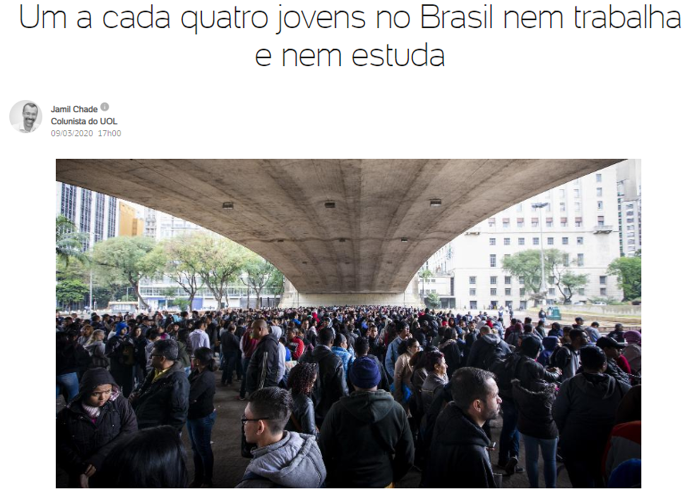
\includegraphics[width=350bp]{financeira4}

\caption{\small SÃO PAULO, SP, BRASIL, 06/08/2018, 10h00. Especial desemprego: Pessoas em busca de uma vaga de emprego formam filas nas proximidades do Sindicato dos Comerciários de São Paulo, no Vale do Anhangabaú, na região central de SP. Devido ao dia chuvoso, as filas se acumulavam embaixo do Viaduto do Chá. O sindicato organiza o 2º Mutirão do Emprego, com o objetivo é oferecer ainda mais oportunidades de trabalho, em postos que tenham remuneração maior.}
\end{figure}

\begin{quote}
Um a cada quatro jovens no Brasil está desempregado, numa realidade que se assemelha aos índices registrados no Norte da África e no Oriente Médio. A taxa está sendo divulgada nesta segunda-feira pela Organização Internacional do Trabalho (OIT), que destaca como a situação na economia brasileira afeta de forma ainda mais severa as jovens.

Em 2013, o desemprego atingia $15{,}7$\% dos jovens de 14 a 24 anos no Brasil. Em 2019, a média subiu para $27{,}8$\%. Para 2020 e 2021, a previsão é de que ela continue elevada, ainda que caindo para $26{,}9$\% e $26{,}$\%, respectivamente.

\flushright Fonte: \href{https://noticias.uol.com.br/colunas/jamil-chade/2020/03/09/um-a-cada-quatro-jovens-no-brasil-nem-trabalha-e-nem-estuda.htm}{UOL Notícias}
\end{quote}

\begin{enumerate}
  \item O título da matéria aponta para um problema social. Qual o principal problema e por que ele acontece no Brasil?
  \item Qual foi o aumento, em pontos percentuais, da taxa de desemprego entre os jovens de 2013 para 2019? E qual foi o aumento percentual dessa taxa de 2013 para 2019? Considere que a população total de jovens seja a mesma nos dois anos.
  \item A imagem é de 2018. A matéria é de março de 2020. Há algum problema nessa diferença entre datas, considerando a mensagem que a matéria tenta transmitir?
\end{enumerate}
\end{task}

\begin{task}{A Pandemia dos preços}
\label{fin-ativ-5}
Durante a pandemia, em 2020, observamos um aumento significativo no preço de vários alimentos e de alguns produtos importados. Isso impactou a vida de pessoas de diferentes classes sociais. Leia atentamente as informações a seguir.

\begin{figure}[H]
\centering

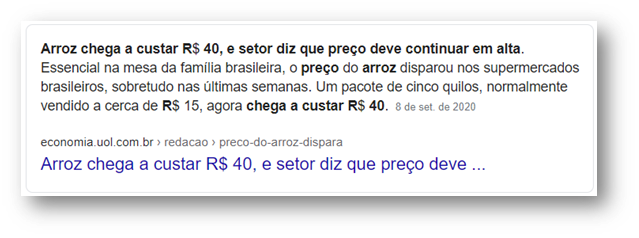
\includegraphics[width=\linewidth]{financeira54}
\caption{Disponível em \href{https://economia.uol.com.br/noticias/redacao/2020/09/08/preco-do-arroz-dispara.html}{Economia UOL}}

\end{figure}

\begin{enumerate}
\item Qual o impacto da alta dos preços dos alimentos de uma maneira geral no orçamento da sua família? Explique um pouco do que aconteceu com ela.
\item Qual foi a variação percentual sofrida pelo preço do arroz, segundo os dados apresentados?
\item Por que o preço do arroz aumentou tanto?
\item Considerando que o preço atual de R\$ $40{,}00$ sofra uma redução de $5\%$ por semana, na comparação com a semana anterior, qual seria o novo preço após duas semanas sucessivas?
\item Se esse padrão de queda se mantivesse, após quantas semanas, no mínimo, o preço voltaria aos R\$ $15{,}00$?
\end{enumerate}
\end{task}


\begin{paginatexto}{Orçamento e planejamento financeiro}

\subsection*{Objetivo geral}

\begin{itemize}
\item Abordar noções de orçamento e planejamento financeiro, em nível pessoal e familiar

\item Conceitos abordados: orçamento e planejamento; média aritmética simples; porcentagem; através das habilidades
\end{itemize}

\begin{habilities}{EM13MAT101}
 Interpretar situações econômicas, sociais e das Ciências da Natureza
que envolvem a variação de duas grandezas, pela análise dos gráficos das funções representadas e das taxas de variação com ou sem apoio de tecnologias digitais.

\tcbsubtitle{EM13MAT203}
Planejar e executar ações envolvendo a criação e a utilização de aplicativos, jogos (digitais ou não), planilhas para o controle de orçamento familiar, simuladores de cálculos de juros compostos, dentre outros, para aplicar conceitos matemáticos e tomar decisões. 

\end{habilities}

\subsection*{Recomendações para o professor}

\paragraph{Organização em sala de aula} esse á um tema que pode ser trabalhado em turmas do Ensino Fundamental e do Médio. Começar com a pergunta: quanto você custa mensalmente? Pode ser um caminho interessante, porque convida o aluno a pensar nas mais variadas categorias de despesas, no valor do trabalho, na adequação da renda às despesas. Coletar informações sobre o orçamento das famílias exige cuidado para não causar constrangimentos, mas precisa ser discutida de forma responsável e adquada à idade.

\paragraph{Dificuldadade previstas} em relação aos aspectos matemáticos, os conceitos são simples, não havendo complexidades significativas, pois envolve as quatros operações elementares com números racionais e porcentagem. O uso da calculadora pode ajudar e muito nessa abordagem.

\paragraph{Sugestões gerais} uma possibilidade para se abordar esse tema é, quando estiver trabalhando conceitos como porcentagem, números racionais ou ainda conceitos de estatística, o professor pode aproveitar sua programação para trabalhar com orçamento e planejamento financeiro em qualquer série ou cicle, conforme a sua disponibilidade e vontade.

As atividades aqui do livro aberto sobre o tema são ricas e variadas, e muitas delas podem ser aplicadas diretamente já no Ensino Fundamental. Cabe ao professor avaliar e/ou adaptar para a sua realidade.

Leve em consideração, sempre que puder, o contexto sócio-econômico dos estudantes na abordagem desse tema. As atividades que levam em consideração, podem produzir um nível de engajamento e pertencimento bem maior do que lidar somente com orçamentos e planejamentos que lhes são tão distantes, com consumos totalmente irreais naquele momento.

A parte de estatística que pode ser (não necessariamente tem que ser) trabalhada, tais como média, média móvel, série histórica (despesas com luz, gás, telefone), pode ser um ponto de dificuldade. Todavia, tem enorme potencial de aplicação e de compreensão das regularidades e sazonalidades das receitas e despesas pessoais e familiares.

\subsection*{Enriquecimento da discussão}

Esse é u'm ótimo tema para se usar ferramentas digitais para organizar e analisar dados, dentre eles destacamos as planilhas eletrônicas. Sugerimos que a inserção no mundo das planilhas pode ser feita por meio da abordagem desse tema. Temos uma excelente oportunidade de usar planilha para aprender noções de planejamento e orámento, e ao mesmo tempo, investigar situações financeiras para aprender ou reforçar noções matemáticas e desenvolver habilidades de construção de planilhas eletrônicas.

As operações são geralmente simples, e a estrutura tabular, juntamente com a lógica dos comandos básicos, pode ajudar na construção de orçamentos e a investigar problemas e soluções.

Por fim, sugerimos o livro \textit{Preciso me planejar} de \cite{zentgraf2015}, bem como ouvir os podcasts do Mauro Halfeld no blog CBN Dinheiro, disponível em \url{https://www.podbean.com/podcast-detail/k9y47-4173d/CBN-Dinheiro---Mauro-Halfeld-Podcast}

\end{paginatexto}

\explore{Orçamento e Planejamento Financeiro}
\label{fin-exp-2}

Quantos cursos você planeja fazer esse ano? Quantos livros pretende ler? Onde quer estar profissionalmente daqui a 5 anos? Qual a sua meta pessoal para melhorar a saúde? Quantas horas de estudo serão necessárias para ingressar na graduação daquela Universidade Pública que você tanto deseja? Quantas pessoas quer influenciar e ajudar na próxima semana? Participará de algum projeto ou ação social, de maneira voluntária, doando seu tempo e sua atenção a alguém que ama, ou simplesmente não conhece, mas que precisa? Para onde vai viajar, e como vai conseguir fazer isso? Quanto de dinheiro vai precisar para realizar seus desejos? 

O ser humano é movido por desejos, buscando atender necessidades das mais variadas. Mas você pensa nos desejos que têm, na relevância deles para a sua vida? Qual o tamanho da sua vontade? Ela é compatível com o tamanho dos teus sonhos e projetos? E qual é o tamanho da sua vontade para planejar as ações e realizar ou ajustar aquilo que foi planejado para atingi-los? 

Uma das oportunidades que a Educação Financeira oferece às pessoas é refletir sobre orçamento e planejamento financeiros, visando a realização de desejos em diversas áreas da vida. Entenda que Planejamento financeiro não é uma mágica. Muito menos para enriquecer. Na prática, significa reunir conhecimentos e técnicas que levam a decisões mais racionais de consumo, investimento, poupança e financiamento, garantindo como resultado uma vida confortável e sem atropelos de última hora.

Queremos convidar você a refletir e entender que todo mês há receitas (entradas de recursos) e despesas (saídas de recursos) que precisam ser organizadas e pensadas. Entender esse fluxo de receitas e despesas pode ajudar as pessoas nas decisões que precisarão tomar para que os sonhos e projetos ganhem alguma chance de serem realizados. 

Para a maioria das pessoas, sem planejamento, estratégia, sacrifícios e esperas, essa chance pode ser muito pequena. E a matemática é um dos aspectos que podem ajudar, e muito, nesse planejamento e consequentemente na definição e realização de metas de curto, médio e longo prazos. Vamos refletir nessa seção sobre orçamento e planejamento financeiro, nas perspectivas pessoal e familiar, buscando construir novas formas de pensar nossos projetos e sonhos, e ter as atitudes que sejam compatíveis com eles.
\clearpage
\begin{objectives}{Como gasto o meu dinheiro?}
{
\begin{itemize}
\item Investigar situações financeiras que envolvem orçamento, planejamento e gestão financeira, tanto a pessoal quanto a familiar.
\item Resolver problemas relacionados ao orçamento e planejamento financeiro. 
\end{itemize}
}{1}{2}
\end{objectives}
\begin{sugestions}{Como gasto o meu dinheiro?}
{
Nessa atividade convidamos o aluno a pensar o peso da alimentação no orçamento das famílias. Em tom de humor, onde um gráfico de setores simula a figura do jogo “pacman” comendo o dinheiro da família, a imagem busca trazer para a discussão como os alimentos acabam comprometendo, juntamente com os custos com habilitação, uma boa parte do orçamento de milhões de famílias. 

Por outro lado, há algumas imperfeições ou pelo menos alguns questionamentos ao peso de outros grupos. Por exemplo, no item b queremos discutir se os transportes costumam ter o mesmo que habitação? Ainda que seja algo que possa acontecer, não nos parece que seja o mais comum. A presença de perguntas abertas amplia as oportunidades de discussão. O objetivo aqui não é fazer contas ainda, mas trabalhar a comparação e o peso de grandes grupos de despesas. Outros gráficos, com informações que contemplem o perfil das famílias dos alunos são muito importantes para o envolvimento dos alunos e na identificação deles com as suas próprias questões, problemas e soluções de orçamento e de planejamento.

Recomendamos uma ampliação dessa atividade que é perguntar aos alunos quanto eles custam por dia? E por mês? Essa atividade costuma trazer surpresas e questionamento dos mais interessantes e inusitados possíveis.

}{0}{2}
\end{sugestions}
\begin{objectives}{Crise à vista: hora de apertar o cinto!}
{
\begin{itemize}
\item Investigar situações financeiras que envolvem orçamento, planejamento e gestão financeira, tanto a pessoal quanto a familiar.
\item Construir propostas e soluções alternativas como apoio para a tomada de decisão em situações envolvendo orçamentos e planejamentos financeiros, considerando aspectos matemáticos e não matemáticos. 
\end{itemize}
}{1}{2}
\end{objectives}
\begin{sugestions}{Crise à vista: hora de apertar o cinto!}
{
Nessa atividade convidamos o aluno a pensar numa possível redução abruta da renda, diante da redução de salário e/ou demissão de um dos membros da família. O contexto é da crise gerada pela Pandemia. 

A atividade é simples nos dados, mas pode ser bem complexa na construção de soluções, uma vez que lidar com uma redução de $40\%$ nas receitas seria um enorme desafio para grande parte das famílias brasileiras. Queremos convidar o estudante a elencar as necessidades mais básicas e prioritárias na opinião deles. 

Seria possível pensar em soluções sem identificar quais são os principais gastos da família? Ou seja, seria possível dar soluções sem fazer um orçamento familiar para reestruturar um planejamento financeiro? 

}{1}{2}
\end{sugestions}
\begin{answer}{Como gasto o meu dinheiro?}
{
\begin{enumerate}
\item Resposta pessoal.
\item Resposta pessoal. Veja o comentário sobre a intenção dessa pergunta
\item Resposta pessoal. Veja a sugestão de variação da atividade proposta.
\item Resposta pessoal. Observe que essa atividade pode ser perfeitamente usada no Ensino Fundamental, talvez a partir do sétimo ano.
\end{enumerate}

\tcbsubtitle{Crise à vista: hora de apertar o cinto!}
Resposta pessoa. Pergunta aberta.
}{0}
\end{answer}

\begin{task}{Como gasto o meu dinheiro?}
\label{fin-ativ-6}

Analise a charge a seguir, publicada em 06/10/2019, na Folha de São Paulo.

\begin{figure}[H]
\centering
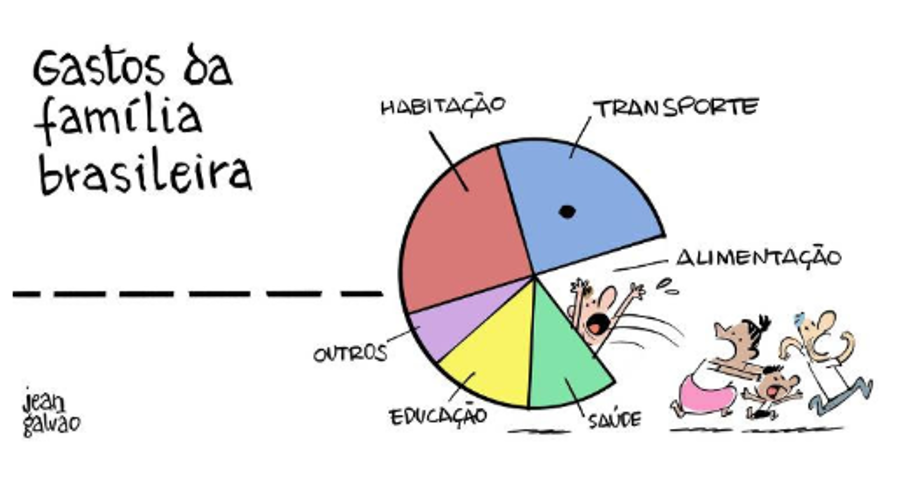
\includegraphics[width=420bp]{charge-gastos.png}

\end{figure}

\begin{enumerate}
\item Qual a principal mensagem que essa charge tenta transmitir?
\item Habitação e transporte costumam ter o mesmo peso no orçamento da sua família?
\item Quanto seus pais gastam com a tua Educação mensal?
\item Estime o percentual que a alimentação representa na renda familiar de acordo com o gráfico apresentado.

\end{enumerate}
\end{task}

Na atividade anterior, o gráfico apresentou várias informações a respeito do orçamento de uma família. Apesar da ideia principal que o artista tentou passar ser o peso da alimentação no consumo da família, que em muitos casos “come” a maior parte dos salários das pessoas, temos ali outras fontes de gastos, tais como habitação, transporte, educação, vestuário. Mas tão importante quanto trabalhar para melhorar nossa renda, é identificar como gastamos nosso dinheiro (diagnóstico), para que possamos decidir o que queremos e podemos fazer com os nossos recursos (planejamento). 


\begin{task}{Crise à vista: hora de apertar o cinto!}
\label{fin-ativ-7}

Com a crise econômica existente no país e também no Estado do Rio de Janeiro, muitas pessoas ficaram desempregadas. Imagine que sua família tivesse uma renda de $5.000$, e devido à crise diminuísse para $3.000$ reais. O que você sugeriria para seus responsáveis em relação a essa nova realidade?
\end{task}

\arrange{Diagnóstico e Plano de Ação}
\label{fin-arg-2}

Veja que um \textbf{orçamento financeiro pessoal} é como um diagnóstico, ou seja, um detalhamento das receitas e despesas de uma ou mais pessoas, em um determinado intervalo de tempo (geralmente mensal), para se identificar de onde vem e para onde vai o dinheiro da família. Da família. Mesmo que você não ganhe, com certeza você gasta. Por isso deve ter responsabilidades e deveres nessa história. E aprender a pensar nisso desde cedo, e aos poucos.

Assim, um orçamento envolve tanto a identificação das fontes de entrada de dinheiro, tais como salários, horas extras, “bicos”, mesadas, presentes em dinheiro, dentre outras, bem como as de saída, geralmente categorizadas em despesas com lazer, alimentação, moradia, vestuário, etc. Tabelas ou aplicativos ajudam na elaboração de um orçamento doméstico.

A partir de um orçamento, ou seja, do diagnóstico das receitas e despesas, pode-se avaliar como cada pessoa ou até mesmo toda a família está gastando o dinheiro, e buscar ajustar as despesas. Pode-se também pensar e agir para aumentar as receitas, com algum trabalho extra, por exemplo, para se atingir alguns objetivos. O objetivo em um mês pode ser simplesmente não gastar mais do que ganha. Em outros meses, pode ser gastar menos do que ganha, para com o que sobra realizar um sonho, fazer uma viagem, ou quem sabe para comprar algum bem que seja importante para a família, como por exemplo uma casa própria no futuro. Assim, chamamos de planejamento financeiro a um conjunto de ações e atitudes que visam organizar a vida financeira, a partir de objetivos bem definidos, chamamos \textbf{planejamento financeiro}. 

Nessa visão, \textbf{planejamento financeiro} se refere a um plano de ações, isto é, ao que quero, posso e devo fazer diante de um orçamento para se atingir determinados objetivos traçados por uma ou mais pessoas. Obviamente o planejamento financeiro pode começar com uma decisão de reorganizar as finanças ou atingir um objetivo específico – como poupar dinheiro para a realização de um curso, para empreender um pequeno negócio, para a cirurgia de alguém da família, ou para a compra de um bem (carro, casa, etc) – a partir do qual segue-se um orçamento que vai ajudar a mapear a situação financeira, para que o planejamento possa ser de fato executado, posto em prática.

\vspace{-.75em}
\begin{knowledge}

\begin{wrapfigure}[10]{r}{.2\textwidth}
\vspace{-1em}
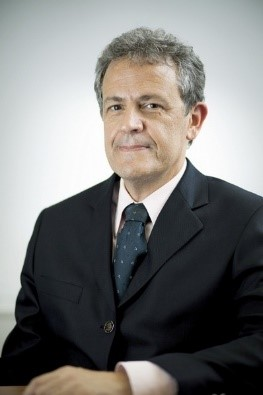
\includegraphics[width=.2\textwidth]{financeira25}
\end{wrapfigure}
Planejamento financeiro não é uma mágica. Muito menos para enriquecer. Na prática, significa reunir conhecimentos e técnicas que levam a decisões mais racionais de consumo, investimento, poupança e financiamento, garantindo como resultado uma vida confortável e sem atropelos de última hora. Boa parte das dificuldades para planejar as finanças tem origem em questões comportamentais, como o consumo excessivo. Para pessoas que compram demais, por exemplo, o esforço é muito mais no campo da atitude do que no da técnica de planejamento. Mas não é só o comportamento que justifica toda a questão. Tem muita gente que não compreende corretamente os fundamentos do ambiente econômico, ficando assim à mercê de situações que são, no mínimo, desfavoráveis.
\end{knowledge}
\vspace{-.5em}

Assim temos duas ideias que se complementam, que podem e devem ser postas em ação numa relação praticamente simbiótica, e que entendemos ser muito importante na vida financeira das pessoas, uma vez que um diagnóstico pode ajudar o indivíduo, e/ou sua família, a entender o movimento do dinheiro, contribuindo para identificar possíveis desperdícios, reavaliar prioridades, identificar os candidatos a cortes, ampliar as receitas, estimar o tempo necessário para se atingir determinadas metas, dentre outras ações.

\subsection{Mas como montar um orçamento financeiro? Por onde começar?}

A primeira etapa é o \textbf{registro}, onde deve-se coletar os extratos, boletos pagos, cupons fiscais, contracheque, faturas, recibos de aluguel e outros documentos que comprovem o que foi gasto ou recebido naquele mês.

Depois vem a \textbf{consolidação}. Classifique os valores em salário, alimentação, lazer, aluguel etc. Organize os dados e faça gráficos de pizza ou barras para essas áreas do seu orçamento. Com isso você terá mapeado suas despesas e receitas, fechando o teu diagnóstico.

Agora é preciso pensar nos planos e nas ações. Vamos aos planos!

A \textbf{análise} é a fase mais importante, pois é onde você vai usar a cabeça para descobrir onde tem gasto mais, a evolução de seus ganhos e despesas etc. É aqui que você decide onde cortar e como ganhar mais.   

A última etapa é a \textbf{previsão}. Planeje seu futuro financeiro, usando os sonhos que você traçou como guia para estabelecer as metas, que devem ser viáveis, factíveis, porém desafiadoras

O esquema a seguir mostra uma sugestão de etapas para a elaboração de um orçamento financeiro. 

\begin{figure}[H]
\centering
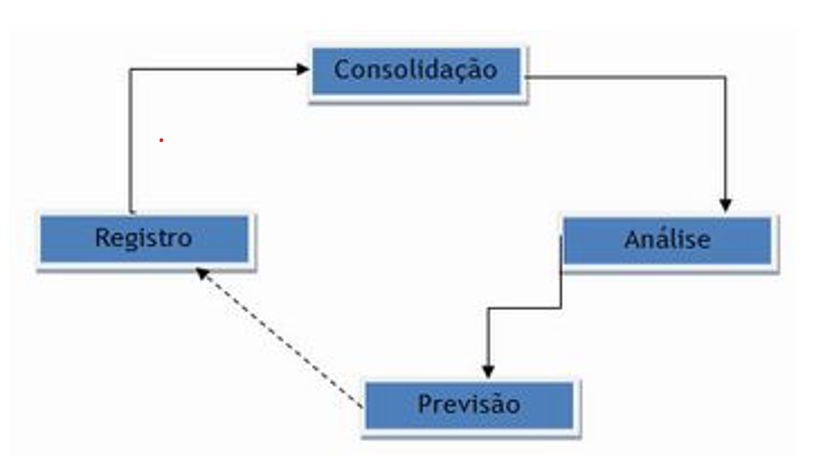
\includegraphics[width=350bp]{fluxograma-previsao}

\caption{\cite{zentgraf2015}}
\end{figure}

Você entendeu a diferença entre o orçamento e o planejamento? Enquanto o orçamento mostra um retrato (diagnóstico) das entradas e saídas do dinheiro que a família ganha, o planejamento financeiro (plano de ações) é o que a família vai fazer, em termos de ações, atitudes e decisões para se atingir objetivos que a própria família entende ser importantes atingir. 

\clearpage
\begin{objectives}{O enigma das despesas invisíveis}
{
\begin{itemize}
\item Investigar situações financeiras que envolvem orçamento, planejamento e gestão financeira, tanto a pessoal quanto a familiar.
\item Resolver problemas relacionados ao orçamento e planejamento financeiro. 
\item Construir propostas e soluções alternativas como apoio a tomada de decisão em situações envolvendo orçamentos e planejamentos financeiros, considerando aspectos matemáticos e não matemáticos. 
\end{itemize}
}{1}{1}
\end{objectives}
\begin{sugestions}{O enigma das despesas invisíveis}
{
Nessa atividade convidamos o aluno a pensar no orçamento da própria família. E a buscar investigar quanto ele custa por mês. Com isso o estudante é convidado a elaborar um orçamento, a identificar como a família gasta o dinheiro e de qual o papel dele nesses gastos. Essas reflexões costumam trazer perplexidade, espantos e curiosidades. Convide seu aluno a construir novas atitudes, alinhadas a objetivos saudáveis, éticos e sustentáveis, que lhe proporcionem atingir metas que sem tais atitudes não seriam possíveis de serem alcançadas. A atividade também pode ajudar o estudante a entender, na medida em que constrói o orçamento da família, as quatro fases que acabamos de apresentar.
}{1}{1}
\end{sugestions}
\begin{answer}{O enigma das despesas invisíveis}
{
\begin{enumerate}
\item Resposta pessoal.
\item Resposta pessoal. Veja o comentário sobre a intenção dessa pergunta
\item Resposta pessoal. Veja a sugestão de variação da atividade proposta.
\item Resposta pessoal. Observe que essa atividade pode ser perfeitamente usada no Ensino Fundamental, talvez a partir do sétimo ano.
\end{enumerate}
}{1}
\end{answer}
\begin{task}{O enigma das despesas invisíveis}
\label{fin-ativ-8}

Douglas é um estudante da 2ª série do Ensino Médio de um Colégio Estadual no Rio de Janeiro. 

Ao assistir uma matéria no telejornal sobre a crise financeira no país, decidiu perguntar aos pais quanto que gastavam com ele em um mês. Mesmo sem ter um emprego, ele pensou que de alguma maneira poderia ajudar os pais com as despesas da casa. Os pais propuseram fazer um orçamento com os valores dos gastos da família, somar tudo e depois dividir por cinco, pois Douglas mora com os pais e dois irmãos menores de idade. 

No orçamento eles colocaram os valores de alimentação, telefone, luz, plano de saúde, prestação do carro, cartão de crédito e transporte e verificaram que a despesa total era de R\$ 3.500{,}00. Ao fazer a divisão desse valor pela quantidade dos membros da família, Douglas levou um susto, pois não fazia ideia de que seus pais gastavam R\$ 700{,}00 com ele por mês, aproximadamente.  

E você, sabe quanto custa por mês? Utilize a tabela abaixo como referência e descubra quanto você custa por mês e depois responda às questões:

\begin{table}[H]
\centering
\setlength\tabcolsep{15pt}
\begin{tabular}{|l|r|}
\hline
\tmcol{2}{|c|}{Despesas} \\
\hline
\tcolor{Descrição} & \tcolor{Valor} \\
\hline
Alimentação & \\
\hline
Luz & \\
\hline
Água & \\
\hline
Telefone & \\
\hline
Plano de saúde & \\
\hline
Aluguel & \\
\hline
Cartão de crédito & \\
\hline
Lazer & \\
\hline
Educação & \\
\hline
Transporte & \\
\hline

Total & \\
\hline
\end{tabular}
\end{table}

\begin{enumerate}

\item A partir dos dados que você preencheu, determine o custo mensal que sua família tem com você.
\item Em sua opinião, esse valor de custo individual é muito, pouco ou razoável? Justifique.
\item Se você pudesse ajudar a tua família na organização das despesas, o que mudaria?
\item Quais itens que você tiraria ou acrescentaria na tabela a fim de melhorar o controle de gastos em tua família?

\end{enumerate}

\end{task}

\clearpage
\begin{objectives}{Bola de neve}
{
\begin{itemize}
\item Investigar situações financeiras que envolvem orçamento, planejamento e gestão financeira, tanto a pessoal quanto a familiar.
\item Resolver problemas relacionados ao orçamento e planejamento financeiro. 
\item Construir propostas e soluções alternativas como apoio a tomada de decisão em situações envolvendo orçamentos e planejamentos financeiros, considerando aspectos matemáticos e não matemáticos. 
\end{itemize}
}{1}{2}
\end{objectives}
\begin{sugestions}{Bola de neve}
{
Nessa atividade convidamos o aluno a pensar em uma situação na qual uma jovem busca entender o orçamento da família para tentar construir um plano que vise corrigir alguns desiquilíbrios financeiros.

O problema envolve duas partes. Na primeira parte temos uma investigação buscando entender quais são os problemas e onde eles estão. Já na segunda parte há uma questão interessante em que o saldo devedor sofre um reajuste que não é mencionado no texto. Cabe ao aluno tentar entender que se trata de possíveis juros, descobrir qual é a taxa e investigar o impacto disso na ampliação da dificuldade em resolver o problema com essa “bola de neve”. 

}{1}{2}
\end{sugestions}
\begin{answer}{Bola de neve}
{
\begin{enumerate}
\item Resposta pessoal. O aluno precisará identificar pontos onde ele entende ser possível cortar gastos para equilibrar o orçamento. Ele também pode sugerir que alguma ação para aumentar a renda da família.
\item O padrão observado na sequência dos saldos devedores aponta para uma cobrança de juros de $10\%$ ao mês, que pode estar associado ao uso do cheque especial. Considerando esse padrão, o saldo devedor em abril será de 770 reais, uma vez que a diferença entre as receitas e as despesas foi de 700 reais, que atualizada em $10\%$, transformar-se-á em $770$ reais.
\end{enumerate}
}{1}
\end{answer}
\begin{task}{Bola de neve}
\label{fin-ativ-9}

Mariana é uma adolescente muito estudiosa que mora com seu pai, sua mãe e um irmão mais novo de 10 anos. Essa família tem uma renda mensal fixa de 3.500 reais. Para melhorar as finanças da família, eles resolveram elaborar um orçamento doméstico. Para isso, registraram todos os gastos da família nos meses de janeiro, fevereiro e março de 2019. O resultado está apresentado nos quadros a seguir, com os valores em reais. 

\begin{table}[H]
\centering
\setlength\tabcolsep{2.5pt}
\begin{tabular}{|l|r|l|r|l|r|}
\hline
\tmcol{2}{|c|}{Janeiro}& \tmcol{2}{c}{Fevereiro} & \tmcol{2}{|c|}{Março}\\
\hline
\tmcol{1}{|c|}{Descrição} & \tmcol{1}{|c|}{Valor} & \tmcol{1}{c|}{Descrição} & \tmcol{1}{c|}{Valor}& \tmcol{1}{c|}{Descrição} & \tmcol{1}{c|}{Valor}\\
\hline
Alimentação & 900{,}00 & Alimentação & 1000{,}00 & Alimentação & 1060{,}00 \\
\hline
Luz & 120{,}00 & Luz & 150{,}00 & Luz & 170{,}00 \\
\hline
Água & 50{,}00 & Água & 80{,}00 & Água & 90{,}00 \\
\hline
Telefone & 150{,}00 & Telefone & 150{,}00 & Telefone & 150{,}00 \\
\hline
Plano de saúde & 600{,}00 & Plano de saúde & 600{,}00 & Plano de saúde & 600{,}00 \\
\hline
Alguel & 800{,}00 & Alguel & 800{,}00 & Alguel & 800{,}00 \\
\hline
Cartão de Crédito & 350{,}00 & Cartão de Crédito & 120{,}00 & Cartão de Crédito & 240{,}00 \\
\hline
Lazer & 180{,}00 & Lazer & 70{,}00 & Lazer & 50{,}00 \\
\hline
Educação & 400{,}00 & Educação & 400{,}00 & Educação & 400{,}00 \\
\hline
Transporte & 250{,}00 & Transporte & 200{,}00 & Transporte & 200{,}00 \\
\hline
\parbox[c][1cm]{3.25cm}{ Saldo devedor do mês anterior} & 0{,}00 & \parbox[c][1cm]{3.25cm}{ Saldo devedor do mês anterior} & 330{,}00 & \parbox[c][1cm]{3.25cm}{ Saldo devedor do mês anterior} & 440{,}00 \\
\hline
\tcolor{Total} & \tcolor{3800{,}00} & \tcolor{Total} & \tcolor{3900{,}00} & \tcolor{Total} & \tcolor{4200{,}00} \\
\hline
\end{tabular}
\caption{Fonte: Adaptado de \cite{santana2019}}
\end{table}

\begin{enumerate}
\item Quais os problemas de orçamento que você identifica ao ver os gastos dessa família nesses três meses?
\item Qual será o saldo devedor para abril, mantido o padrão observado nos meses anteriores. (Explique que padrão é esse em termos de porcentagem). Por que isso está acontecendo e quais sugestões você daria para essa família?
\end{enumerate}
\end{task}

\clearpage
\def\currentcolor{session2}
\begin{objectives}{Sonhos de uma bolsista}
{
\begin{itemize}
\item Investigar situações financeiras que envolvem orçamento, planejamento e gestão financeira, tanto a pessoal quanto a familiar.
\item Resolver problemas relacionados ao orçamento e planejamento financeiro. 
\item Construir propostas e soluções alternativas como apoio a tomada de decisão em situações envolvendo orçamentos e planejamentos financeiros, considerando aspectos matemáticos e não matemáticos. 
\end{itemize}
}{1}{1}
\end{objectives}
\begin{sugestions}{Sonhos de uma bolsista}
{
Nessa atividade convidamos o aluno a pensar sobre o que faria com seu próprio orçamento se fosse um aluno(a) bolsista, ou seja, se pudesse gerenciar totalmente seu próprio dinheiro proveniente de uma bolsa. A questão das trocas intertemporais aparece aqui. Satisfazer a pequenos desejos todo mês, ou ter paciência e força de vontade para guardar dinheiro para satisfazer a um sonho maior?
}{1}{1}
\end{sugestions}
\begin{answer}{Sonhos de uma bolsista}
{
  Ambas as respostas são individuais
}{1}
\end{answer}
\begin{objectives}{Vivendo a vida no \textit{Slackline}}
{
\begin{itemize}
\item Investigar situações financeiras que envolvem orçamento, planejamento e gestão financeira, tanto a pessoal quanto a familiar.
\item Resolver problemas relacionados ao orçamento e planejamento financeiro. 
\item Construir propostas e soluções alternativas como apoio a tomada de decisão em situações envolvendo orçamentos e planejamentos financeiros, considerando aspectos matemáticos e não matemáticos. 
\end{itemize}
}{1}{1}
\end{objectives}
\clearmargin
\begin{sugestions}{Vivendo a vida no \textit{Slackline}}
{
\begin{wrapfigure}{r}{.3\linewidth}
\vspace{-1em}
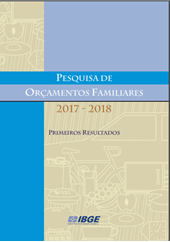
\includegraphics[width=\linewidth]{financeira-professor15}
\end{wrapfigure}
Nessa atividade convidamos o aluno a pensar sobre a dinâmica da frequência do endividamento que algumas pessoas acabam se acostumando, ou dependendo, diante dos desafios de fechar as contas no final do mês, principalmente aquelas mais simples e com faixa salarial próxima a dois salários mínimos, o que corresponde a aproximadamente 45 milhões de pessoas no Brasil, conforme a última Pesquisa de Orçamentos Familiares 2017-2018, publicada em 2019 pelo Instituto Brasileiro de Geografia e Estatística (IBGE), disponível no site pelo link: \url{https://biblioteca.ibge.gov.br/visualizacao/livros/liv101670.pdf}

A análise de vários meses permite ter uma fotografia sobre hábitos de consumo, o que pode ajudar tanto na qualidade como na precisão na busca de soluções e na tomada de decisões para equilibrar as contas.
}{1}{2}
\end{sugestions}


\begin{answer}{Vivendo a vida no \textit{Slackline}}
{
  As respostas são individuais. 

  Inserimos novamente nessa atividade uma cobrança de juros sobre o saldo devedor. Não existe almoço grátis, e os juros impactam no orçamento das famílias brasileiras.
}{1}
\end{answer}

\practice{Orçamento e Planejamento Financeiro}
\label{fin-prac-2}

\begin{task}{Sonhos de uma bolsista}
\label{fin-ativ-10}

Adrieny tem 15 anos e é aluna da 1ª série do Ensino Médio em uma escola pública no Rio de Janeiro. Ela participa de um programa de iniciação científica nessa escola, e por isso ganha uma bolsa de iniciação científica júnior no valor de R\$100{,}00, durante 8 meses, se cumprir satisfatoriamente todas as tarefas solicitadas, ao longo desse tempo. Considerando que a aluna não paga passagem e nem alimentação no período em que está na escola, responda aos itens abaixo.

\begin{enumerate}
\item O que você faria no primeiro mês com esses R\$100 se estivesse no lugar de Júlia? Monte uma tabela com seu orçamento nesse mês
\item O que você faria ao longo dos oito meses, com o dinheiro que fosse recebendo?
\end{enumerate}
\end{task}

\begin{task}{Vivendo a vida no \textit{Slackline}}
\label{fin-ativ-11}
\textit{Adaptado de \cite{santana2019}}

O esquema abaixo representa o registro de uma pessoa, sem filhos,  que recebe um salário de $1.502$ reais por mês.

\begin{table}[H]
\centering
\setlength\tabcolsep{1.5pt}
\begin{tabular}{|l|r|r|r|r|r|r|}
\hline
\tcolor{} & \tmcol{1}{l|}{JAN} & \tmcol{1}{l|}{FEV} &\tmcol{1}{l|}{MAR} & \tmcol{1}{l|}{ABRIL} & \tmcol{1}{l|}{MAIO} & \tmcol{1}{l|}{JUN} \\
\hline
Salário &\textcolor{session2}{\textbf{R\$1.502{,}00}} & \textcolor{session2}{\textbf{R\$1.502{,}00}} & \textcolor{session2}{\textbf{R\$1.502{,}00}} & \textcolor{session2}{\textbf{R\$1.502{,}00}} & \textcolor{session2}{\textbf{R\$1.502{,}00}} & \textcolor{session2}{\textbf{R\$1.502{,}00}} \\
\hline
Comida & \textcolor{session3}{\textbf{-R\$ 273{,}00}} & \textcolor{session3}{\textbf{-R\$ 252,95}} & \textcolor{session3}{\textbf{-R\$ 320{,}00}} & \textcolor{session3}{\textbf{-R\$ 270{,}00}} & \textcolor{session3}{\textbf{-R\$ 298{,}00}} & \textcolor{session3}{\textbf{-R\$ 335{,}00}} \\ 
\hline
Conta de Luz & \textcolor{session3}{\textbf{-R\$ 350{,}00}} & \textcolor{session3}{\textbf{-R\$ 225{,}00}} & \textcolor{session3}{\textbf{-R\$ 212{,}00}} & \textcolor{session3}{\textbf{-R\$ 210{,}00}} & \textcolor{session3}{\textbf{-R\$ 232{,}00}} & \textcolor{session3}{\textbf{-R\$ 210{,}00}} \\ 
\hline
Conta de Água & \textcolor{session3}{\textbf{-R\$ 250{,}00}} & \textcolor{session3}{\textbf{-R\$ 125{,}00}} & \textcolor{session3}{\textbf{-R\$ 112{,}00}} & \textcolor{session3}{\textbf{-R\$ 110{,}00}} & \textcolor{session3}{\textbf{-R\$ 132{,}00}} & \textcolor{session3}{\textbf{-R\$ 110{,}00}} \\ 
\hline
Transporte & \textcolor{session3}{\textbf{-R\$ 416{,}00}} & \textcolor{session3}{\textbf{-R\$ 423,20}} & \textcolor{session3}{\textbf{-R\$ 420{,}00}} & \textcolor{session3}{\textbf{-R\$ 416{,}00}} & \textcolor{session3}{\textbf{-R\$ 416{,}00}} & \textcolor{session3}{\textbf{-R\$ 417,20}} \\ 
\hline
Lazer/Outros & \textcolor{session3}{\textbf{-R\$ 875{,}00}} & \textcolor{session3}{\textbf{-R\$ 163{,}00}} & \textcolor{session3}{\textbf{-R\$ 762{,}00}} & \textcolor{session3}{\textbf{-R\$ 10{,}00}} & \textcolor{session3}{\textbf{-R\$ 900{,}00}} & \textbf{-R\$ 0{,}00} \\ 
\hline
Ganhos Extras &\textcolor{session2}{\textbf{R\$20{,}00}} & \textcolor{session2}{\textbf{R\$400{,}00}} & \textcolor{session2}{\textbf{R\$21,85}} & \textcolor{session2}{\textbf{R\$150{,}00}} & \textcolor{session2}{\textbf{R\$303,64}} & \textbf{R\$0{,}00} \\
\hline
Outros Gastos & \textbf{R\$0{,}00} & \textcolor{session3}{\textbf{-R\$ 110{,}00}} & \textbf{R\$0{,}00} & \textbf{R\$0{,}00} & \textbf{R\$0{,}00} & \textcolor{session3}{\textbf{-R\$ 24{,}00}} \\ 
\hline
Dívidas Anteriores & \textbf{R\$0{,}00} & \textcolor{session3}{\textbf{-R\$ 706{,}00}} & \textbf{R\$0{,}00} & \textcolor{session3}{\textbf{-R\$ 332,37}} & \textbf{R\$0{,}00} & \textcolor{session3}{\textbf{-R\$ 189,60}} \\ 
\hline
Saldo & \textcolor{session3}{\textbf{-R\$ 642{,}00}} & \textcolor{session2}{\textbf{R\$21,85}} & \textcolor{session3}{\textbf{-R\$ 302,15}} & \textcolor{session2}{\textbf{R\$303,64}} & \textcolor{session3}{\textbf{-R\$ 172,36}} & \textcolor{session2}{\textbf{R\$126,20}} \\ 
\hline
\end{tabular}
\end{table}

\begin{enumerate}
\item Observe o registro dos gastos de uma pessoa durante 6 meses. É possível notar que ela frequentemente obtém dívidas. Você consegue observar algum outro padrão? Se sim, que padrão é esse? Descreva-o.

\item Você consegue ver qualquer semelhança entre essa situação e a sua realidade? O que você/a sua família normalmente faria para resolver um problema como o apresentado?

\clearpage
\item Preencha o registro a seguir de acordo com o que você acredita que sejam seus gastos.

\end{enumerate}

\begin{table}[H]
\centering
\begin{tabular}{|>{\color{session3}}l|>{\color{session3}}l|}
\hline
\tcolor{Receitas/Despesas} & \tcolor{Valor} \\
\hline
\textcolor{session2}{Salário} & \textcolor{session2}{\hspace{0.3em} R\$ } \\
\hline
Comida & \textcolor{session3}{-R\$ }\phantom{10000{,}00} \\
\hline
Conta de Luz & -R\$  \\
\hline
Transporte & -R\$ \\
\hline
Cinema/Festas/Outros & -R\$  \\
\hline
Material Escolar & -R\$  \\
\hline
Conta de Internet & -R\$  \\
\hline
Conta de Celular & -R\$  \\
\hline
Assinaturas (Netflix, etc) & -R\$  \\
\hline
Cursos & -R\$  \\
\hline
Dívidas Anteriores & -R\$  \\
\hline
Outros Gastos & -R\$  \\
\hline
\textcolor{session2}{Saldo} & \textcolor{session2}{\hspace{0.3em} R\$}  \\
\hline
\end{tabular}
\end{table}
\end{task}




\begin{paginatexto}{O valor do dinheiro no tempo}\raggedcolumns

\subsection*{Objetivo geral}

\begin{itemize}
\item Abordar fatores que transformam o dinheiro no tempo, tais como juros, inflação e câmbio, e a principal forma de transformação.

\item \textbf{Conceitos abordados}: Valor presente e Valor futuro, Progressõies Aritméticas e Geométricas, através das habilidades:
\end{itemize}

\begin{habilities}{EM13MAT101}
 Interpretar situações econômicas, sociais e das Ciências da Natureza
que envolvem a variação de duas grandezas, pela análise dos gráficos das funções representadas e das taxas de variação com ou sem apoio de tecnologias digitais.

\tcbsubtitle{EM13MAT203}
Planejar e executar ações envolvendo a criação e a utilização de aplicativos, jogos (digitais ou não), planilhas para o controle de orçamento familiar, simuladores de cálculos de juros compostos, dentre outros, para aplicar conceitos matemáticos e tomar decisões. 

\tcbsubtitle{EM13MAT507}
Identificar e associar sequências numéricas (PA) a funções afins de domínios discretos para análise de propriedades, incluindo dedução de algumas fórmulas e resolução de problemas.

\tcbsubtitle{EM13MAT508}
Identificar e associar sequências numéricas (PG) a funções exponenciais de domínios discretos para análise de propriedades, incluindo dedução de algumas fórmulas e resolução de problemas.
\end{habilities}

\subsection*{Sugestões e Recomendações}
\paragraph{Organização em sala de aula} Sugerimos que o professor comece sempre perguntando aos alunos o que podem dizer sobre o valor do dinheiro e sobre o que eles desejam hoje e no futuro. As situações econômicas e financeiras apresentadas logo no início da seção são exemplos que podem ser usados também para motivar a discussão inicial. Convidar os estudantes a pesquisarem informações envolvendo SEF em sites, blogs, jornais, portais, revistas econômicas sobre situações envolvendo SER em sites; blogs; jornais; portais; revistas econômicas; revistas econômicas sobre situações envolvendo inflação; antes de abordar o tema, pode ampliar o escopo de coisas a partir das quais poderão produzir significados. Convide seus alunos a criar a cultura de investigar os fundamentos e a razoabilidade das informações veiculadas nas mídias socias de sociais de forma fundamentada.

\paragraph{Dificuldades previstas} Vamos lidar com exponenciais; progressões geométricas; em algum momento logarítmos; raízes de índices variados. O uso da calculadora é indispensável. Diante de dificuldades nos conceitos, vale a pena parar e explicar, ou fazer algum tipo de revisão antes.

\paragraph{Sugestões gerais} Nessa seção, abordaremos um dos conceitos mais importantes em finanças, o valor do dinheiro no tempo. Basicamente, estamos interessados e sbar o porquê de uma quantia hoje pode valer mais (ter mais poder de compra, por exemplo) ou menos no futuro. Analisaremos situações financeiras envolvendo uma das formas de se transformar o dinheiro no tempo: os juros compostos. Lembre-se que vamos considerar os aspectos matemáticos, juntamente com os aspectos não matemáticos, para discutir transformações do dinheiro no tempo, juntamente com possíveis impactos e consequências na vida das pessoas.

Assim, a matemática financeira será uma das ferramentas para se construir educação financeira, e ao mesmo tempo, a investigação de situações financeiras em sala de aula pode gerar boas oportunidades para se aprender matemática, incluindo a matemática financeira.

\subsection*{Enriquecimento da discussão}

Por que o dinheiro se transforma no tempo? Como o dinheiro se transforma no tempo? 

As respostas para essas duas perguntas costumam ser confundidas e reduzidas. Vamos começar esclarecendo a diferença entre as duas.

Na primeira, queremos saber qual a razão do dinheiro se transformar no tempo, ou de uma maneira geral, quais são os fatores que modificam o valor do dinheiro no tempo.

No livro aberto de Educação Financeira, vamos abordar quatro fatores que influenciam a transformação do dinheiro no tempo: juros; inflação; câmbio; investimento.

Na segunda, queremos saber como o dinheiro se transforma no tempo, ou seja, quais os aspectos matemáticos que modelam, explicam e nos permitem saber o valor de uma quantia no futuro a partir de uma quantia no presente, conhecendo-se o tempo, a taxa e outras eventuais informações adicionais, tais como taxas administrativas, seguros, valor da parcela, início do pagamento das parcelas, número de dias úteis, etc.

Esse é o foco dessas seção discutir como determinar o valor futuro a partir do valor presente.

Em juros, por exemplo, nós temos três tipos de transormação: os juros simples, que são diretamente proporcionais ao tempo à taxa de juros e ao capital inicial aplicado; os juros compostos, em que a taxa incide sobre o valor acumulado, e os juros mistos, uma combinação deles, aplicando-se juros compostos e, em seguida ,juros simples.

Perceba que juros são apenas um dos fatores que influenciam na transformação do dinheiro no tempo, e veja que nós não começamos o capítulo por juros. Apresentamos duas situações que sequer mencionam os juros.
\end{paginatexto}


\begin{texto}
{\def\currentcolor{session1}
\subsection{Objetivos específicos}
\begin{itemize}
\item Identificar diferentes fatores que influenciam o valor do dinheiro no tempo, tais como juros, inflação, câmbio, investimentos e percepção de utilidade.
\item Resolver problemas relacionados a juros simples ou compostos
\item Analisar e tomar decisões em situações econômico-financeiras que envolvam o valor do dinheiro no tempo, considerando aspectos matemáticos e não matemáticos.
\end{itemize}

\subsection{Sugestões e discussões}

Aqui apresentamos três atividades que formam um conjunto de situações para iniciarmos a exploração da noção de valor do dinheiro no tempo e suas formas de transformação.
Recomendamos ao professor (a) que leia as orientações no início dessa seção para ampliar a visão sobre o valor do dinheiro no tempo, os diferentes fatores que o influenciam, bem como para não se limitar a achar que abordar o valor do dinheiro no tempo significa ensinar juros simples e juros compostos. 

Nesse conjunto de três atividades, disparamos na primeira atividade um convite a pensar sobre juros em um contexto de investimento no mercado financeiro, onde quantias iguais aplicadas representam retornos completamente diferentes, considerando uma mesma taxa e um mesmo prazo final de resgate. Essa atividade só será de fato resolvida na próxima seção, e faremos um percurso com uma série de problemas mais simples até construirmos as bases para podermos analisa-la de forma completa. Aqui é só um disparo, para coletar impressões e observar diferentes significados produzidos, com operações e lógicas que produzem inicialmente, respostas diferentes das que efetivamente aconteceriam.

Na segunda temos o contexto de inflação e da variação cambial, modificando o valor do dinheiro no tempo, e consequentemente o poder de compra das pessoas, o que pode afetar a vida de um amplo espectro da população brasileira, pois afeta tanto o preço do arroz ou do trigo (com forte impacto na vida da população mais pobre), como o preço de produtos de maior valor agregado, tais como os equipamentos de tecnologia digital.

Finalmente na terceira temos uma discussão sobre pagamento de juros no contexto do atraso do pagamento de uma conta. Que tipo de juros são cobrados? Um convite a pensar em um contexto real sobre juros simples, ainda que tais contextos sejam raros, depois de uma discussão sobre juros compostos, iniciada na primeira atividade, mas efetivamente trabalhada ao longo da seção com problemas inicialmente simples, que se transformam aos poucos em problemas mais complexos.

\subsection{Solução}
A solução comentada será apresentada no próprio texto, dentro do tópico "Organizando as ideias"
}
\end{texto}
\explore{O Valor do Dinheiro no Tempo}
\label{fin-exp-3}
Quando tomamos decisões financeiras, nos mais variados ciclos da vida – da juventude à velhice, passando pela vida adulta – nos deparamos com escolhas intertemporais, ou seja, escolhas relacionadas ao binômio: Sacrifícios $\times$ Benefícios, que acontecem em momentos diferentes no tempo. Desfrutar o momento ou cuidar do amanhã? Assim, trocas intertemporais \citep{fonseca2005} são situações envolvendo escolhas em que valores ou benefícios usufruídos mais cedo acarretam algum tipo de ônus ou custo a ser pago mais à frente. Vejamos alguns exemplos práticos

\begin{itemize}
  \item Contrair ou não um empréstimo para financiar a compra de uma televisão, um carro ou a tão sonhada casa própria?
  \item Pagar no débito ou no crédito?
  \item Comprar um celular novo hoje ou usar o dinheiro para fazer um curso de informática nos próximos seis meses?
  \item Poupar dinheiro no presente para realizar algum sonho ou projeto no futuro (quando isso é possível ou quando o nosso sistema límbico nos permite) ou comprar agora e viver um dia de cada vez sem pensar muito no futuro?
  \item Comprar a passagem agora ou esperar correndo o risco que o preço aumente?
  \item Pagar à vista ou pagar parcelado?
  \item Aproveitar a promoção de produtos de primeira necessidade agora, e ter que se apertar um pouco agora, ou comprar mais caro depois, para não se primvar do que está acostumado?
  \item Investir parte da renda para realizar sonhos a médio ou longo prazos ou viver e gastar sem se preocupar com o futuro?
  \item Investir durante um determinado período da vida para constituir um fundo de reserva para a aposentadoria ou para situações de imprevisto, considerando fatores como aumento da expectativa de vida, a redução da capacidade de trabalho na velhice e os riscos a longo prazo ou ignorar completamente esses aspectos e viver a vida intensamente sem se preocupar com tais questões?
\end{itemize}

Esses são apenas alguns exemplos de trocas intertemporais. Em cada uma dessas situações temos uma ou mais trocas intertemporais, ou seja, trocas envolvendo sacrifícios e benefícios realizados em diferentes momentos no tempo. Nesta seção, convidamos você a entender algumas formas de transformação do dinheiro no tempo e como isso está relacionado a trocas intertemporais presentes em nosso dia a dia.


\clearpage
\begin{task}{Iguais podem ser diferentes?}
\label{fin-ativ-12}

Você tem duas possibilidades de fazer uma poupança:

\begin{itemize}

\item Investir 200 reais por mês durante 20 anos

\item Investir 400 reais por mês durante 10 anos, parar de depositar, deixando o acumulado rendendo até completar o prazo de 20 anos.

\end{itemize}

Considere que o dinheiro renda $1$\% ao mês, rendendo sempre sobre o saldo acumulado da sua poupança. 

\begin{enumerate}

\item Qual a melhor estratégia do seu ponto de vista? Justifique sua resposta.

\item Qual a estratégia que gera o maior valor acumulado ao final de 20 anos?

\item O que isso tem a ver com a discussão atual (2019) sobre a reforma da previdência?
\end{enumerate}

\end{task}

\begin{task}{Inflação: o que eu tenho a ver com isso?}
\label{fin-ativ-13}

Leia atentamente as chamadas de algumas matérias veiculadas na internet sobre o impacto da inflação na vida das pessoas?

\begin{figure}[H]
\centering


\includegraphics[width=365bp]{financeira5}

\caption{Fonte: \href{https://www.destaquenoticias.com.br/panificadores-de-sergipe-prometem-reajustar-preco-do-pao/}{Destaque Notícias}}
\end{figure}

\begin{figure}[H]
\centering

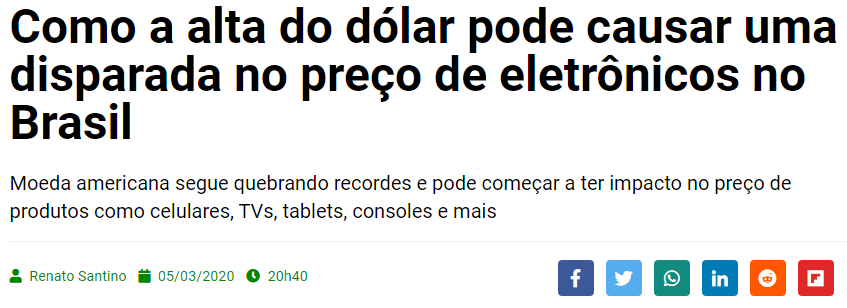
\includegraphics[width=365bp]{financeira6}
\end{figure}
\begin{enumerate}
  \item Você viveu alguma experiência de consumo ou renda, em quem a alta do dólar influenciou na sua vida e da sua família?
  \item A variação cambial pode transformar o dinheiro no tempo? Explique e exemplifique.
\end{enumerate}
\end{task}
\needspace{.1\textheight}
\begin{task}{Passou do vencimento: e agora?}
\label{fin-ativ-14}

José tinha uma conta para pagar no valor de R\$ $1.328{,}78$ com vencimento para 15/06/2019. Entretanto, ele só conseguiu pagar a conta no dia 21/06/2019

\begin{figure}[H]
\centering

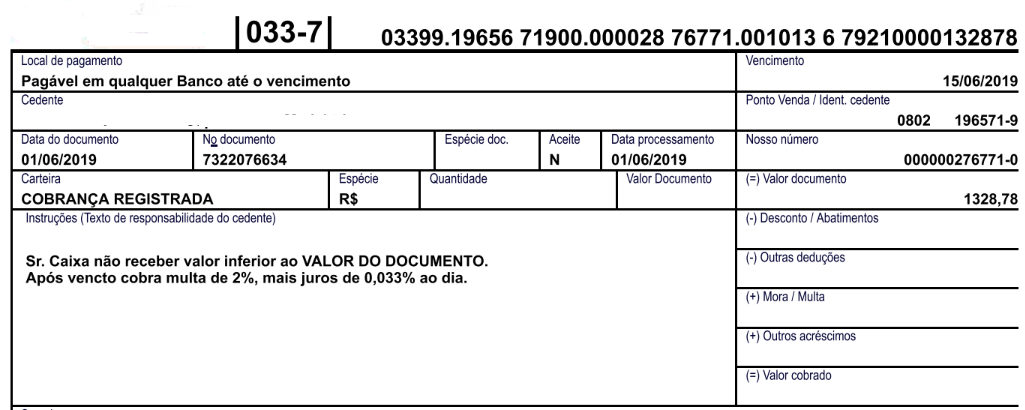
\includegraphics[width=.8\linewidth]{financeira7}
\end{figure}

\begin{enumerate}
  \item O valor da conta muda antes do vencimento? E depois?
  \item Qual o valor pago por José, considerando as instruções apresentadas no boleto acima?
\end{enumerate}
\end{task}

\begin{knowledge}

Mas afinal, o que é dinheiro? O dinheiro é um meio de troca, que tem a vantagem de ser melhor que o escambo (troca de mercadorias por outras mercadorias – galinhas por arroz, madeira por espelhos, etc), pois tem equivalência de valor, o que facilita a avaliação e o cálculo. É também um “recipiente de valor”, que permite que as transações econômicas sejam conduzidas durante longos períodos e por longas distâncias geográficas.

\begin{wrapfigure}[16]{r}{.28\textwidth}
\vspace{-1em}
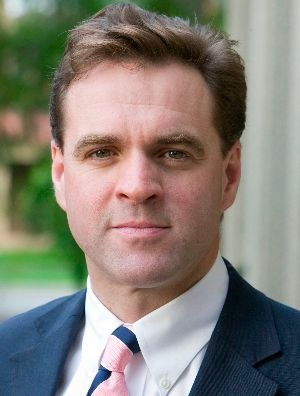
\includegraphics[width=.28\textwidth]{niall-ferguson}

\caption{Niall Ferguson}
\end{wrapfigure}

Segundo o historiador Niall Ferguson, em seu livro A Ascensão do Dinheiro, para desempenhar todas essas funções, o dinheiro tem que estar disponível, ser durável, substituível, portátil e confiável. E ao longo dos séculos, os metais como ouro, prata e bronze foram considerados como a matéria prima monetária ideal. As moedas mais antigas que se conhecem são de aproximadamente 2600 anos atrás (600 a.C) e foram encontradas em uma região da Turquia. 

Independente da forma como os povos têm utilizado para produzir dinheiro, o que realmente importa é que os interessados concordem com o valor acordado e registrado. Se isso for respeitado, o dinheiro cumpre o seu papel. 

Em todo sistema monetário forte, é preciso uma moeda que seja confiável, impressa com padrões de segurança para inibir as falsificações. Para isso, o Brasil dispõe da Casa da Moeda, que em parceria com o Banco Central, tem procurado dotar as cédulas de elementos antifalsificação cada vez mais modernos, contribuindo para a garantia da segurança do dinheiro brasileiro no presente e no futuro.

\end{knowledge}

\arrange{Valor Presente e Valor Futuro}
\label{fin-arg-3}

Antes de começarmos a pensar em valor presente e valor futuro, é importante entender o que é juro. O juro é o quanto se paga para usar o dinheiro que não se tem. É uma espécie de aluguel do dinheiro.

Na primeira atividade, qual a estratégia que seria mais viável (possível) financeiramente para você? Será que ela coincide com a estratégia que gera o maior valor acumulado ao final de 20 anos?

Na segunda atividade, podemos dizer que a variação cambial intervere no valor do dinheiro no tempo, e consequentemente na vida dos cidadãos, com impactos variados?

Na terceira, os juros e o valor após o vencimento são calculados da mesma forma que seriam calculados os juros da primeira atividade?

Convidamos você a investigar, nas próximas páginas, que é possível determinar a melhor estratégia, do ponto de vista financeiro, usando usando um conceito muito importante: o valor do dinheiro no tempo. E também como analisar o impacto da inflação e da variação cambial na transformação do dinheiro no tempo.

Na \textbf{primeira situação}, apesar do total de dinheiro investido ser o mesmo (ou seja, os valores nominais investidos são iguais: $400 \times 120 = 200 \times 240$), eles serão depositados em momentos diferentes. E isso vai gerar valores acumulados em uma mesma data, também diferentes. Depositar quantias maiores antes produz mais dinheiro no futuro do que depositar quantias menores, considerando um mesmo intervalo de tempo total. E isso tem impactos a longo prazo importantes, e tem relação com aspectos prevideciários relevantes para uma população que está vivendo, em média, mais tempo.

\textbf{Para entendermos por que tudo isso acontece, tanto em seus aspectos matemáticos como em alguns não matemáticos, vamos abordar exemplos mais simples, para que, de forma gradual, cheguemos aos modelos matemáticos que nos permitam analisar melhor a situação apresentada na atividade anterior.}

Vamos considerar a seguinte situação financeira. Suponha que Humberto invista R\$ $10.000{,}00$ a uma taxa de $12$\% ao ano, e deixe o \textbf{dinheiro aplicado por cinco anos}. Observe que tempo e taxa estão referidos à mesma unidade de tempo. Ao final desse período, qual será o montante acumulado, considerando que a taxa incida sobre o saldo acumulado a cada ano? (Esse processo, denominado sistema de juros compostos, é o mais usual em aplicações financeiras, e por isso será o primeiro a ser tratado aqui nesse texto).

Aprendemos na seção anterior que, ao aumentarmos uma quantia de uma taxa $i$, a mesma fica multiplicada por um fator de atualização igual a $(1+i)$. Em nosso caso, a cada ano, o valor acumulado ficará multiplicado por $1,12$, uma vez que os aumentos são sucessivos, ou seja, a taxa incide sobre o saldo acumulado até então.

Assim, chamando os $10.000$ reais de \textbf{valor presente (${\mathit{VP}}$)}, indicando que ele está associado ao início do investimento, o \textbf{valor futuro ($\mathit{VF}$)} dessa quantia após um ano será $\mathit{VF} = 10.000\times1{,}12 = 11.200$ reais. Passado mais um ano, teremos um novo valor futuro, dado agora por $\mathit{VF} = 11.200\times1{,}12 = 12.544{,}00$. Observe que como a cada ano o valor futuro é $12\%$ maior que o acumulado do ano anterior, e consequentemente multiplicado por $1{,}12$, o Valor Futuro após exatos cinco anos será igual a:

$$\mathit{VF}=10.000 \times 1,12^5=17.623,42$$

Os juros nesse caso são ditos juros compostos, uma vez que a taxa incide sobre o acumulado. As representações temporais a seguir mostram a transformação dos dez mil reais inicialmente investidos ao longo dos cinco anos, a uma taxa de $12\%$ ao ano aplicada sempre sobre o acumulado até o ano anterior.

\begin{table}[H]
\centering
\begin{tabular}{|c|c|}
\hline
\tcolor{Anos de aplicação} & \tcolor{Valor atualizado}\\
\hline
0 & 10.000{,}00\\
\hline
1 & 11.200{,}00\\
\hline
2 & 12.544{,}00\\
\hline
3 & 14.049{,}00\\
\hline
4 & 15,735,19\\
\hline
5 & 17.623,42\\
\hline

\end{tabular}
\end{table}

\begin{figure}[H]
\centering

\begin{tikzpicture}[yscale=0.5, scale=0.5]

\foreach \x in{2,4,6,8,...,20}  \draw [gray!70, thin] (0,\x) -- (18,\x) node [black, pos=0.0,left] {\x.000{,}00}; 
\draw (0,0) -- (18,0) node [black, pos=0.0,left] {0{,}00};

\foreach \x/\y/\z in {1/10/0,4/11.2/1,7/12.544/2,10/14.049/3,13/15.73519/4,16/17.62324/5} 
{
\draw (\x,0) [fill=\currentcolor] rectangle (\x+1,\y);
\node [below] at (\x+1/2, 0) {\z};
}; 
\node at (9,21.5) {\Large Valor atualizado anual};

\end{tikzpicture}
\end{figure}

Observe que, para cada ano, temos um valor futuro associado aos dez mil reais inicialmente investidos. A cada ano, o valor acumulado é 12\% maior que o acumulado do ano anterior, gerando assim uma progressão geométrica (PG) de termo inicial $10.000$ e razão igual a $1{,}12$.

Além disso, podemos observar que da mesma forma que obtivemos o valor futuro, a partir do valor presente, poderíamos obter o valor presente, a partir do valor futuro. Nesse caso, o problema seria: quanto preciso investir hoje para ter, daqui a cinco anos, a quantia de $17.623{,}42$ reais?

Para isso, bastaríamos realizar a operação inversa, ou seja, fazer: ${\displaystyle \mathit{VP} = \frac{ 17.623{,}42}{ 1{,}12^5} = 10.000}${} reais. O esquema a seguir sintetiza essa reversibilidade por meio da operação inversa àquela realizada anteriormente.


\begin{figure}[H]
\centering

\begin{tikzpicture}[node distance = 4cm, ->]

\node (A) {$10.000{,}00$};
\node (B) [right of=A] {$17.623{,}42$};

\path
(A) edge [color=\currentcolor, very thick, bend left] node [above, black] {$\times1,12^5$} (B)
(B) edge [color=\currentcolor, very thick, bend left] node [black,below]  {$\div 1,12^5$} (A);


\end{tikzpicture}

\end{figure}

Dizemos que $10.000$ reais hoje e $17.623{,}42$ daqui a cinco anos são capitais equivalentes, a uma taxa de $12\%$ ao ano. Um é equivalente ao outro. E esse é mais um exemplo do dinheiro se transformando no tempo, ou seja, o valor de $10.000$ reais se modificando devido aos juros acordados entre quem investiu (que abriu mão de usufruir do dinheiro que tinha durante cinco anos) e quem pagou por esses juros (por ter ficado com os 10.000 reais durante todo esse tempo). 

Um dos pagadores de juros no Brasil é o próprio Estado Brasileiro, que capta dinheiro vendendo títulos públicos.

\begin{figure}[H]

\centering

\includegraphics[width=350bp]{tesouro-direto}
\end{figure}
\vspace{-1em}
\begin{quote}
Ao comprar um título público, você empresta dinheiro para o governo brasileiro em troca do direito de receber no futuro uma remuneração por este empréstimo, ou seja, você receberá o que emprestou mais os juros sobre esse empréstimo. Dessa maneira, com o Tesouro Direto, você não somente se beneficia de uma alternativa de aplicação financeira segura e rentável, como também ajuda o país a promover seus investimentos em saúde, educação, infraestrutura, entre outros, indispensáveis ao desenvolvimento do Brasil. 
\flushright(\href{http://www.tesouro.gov.br/web/stn/-/conheca-o-tesouro-direto}{Fonte: Portal do Tesouro Direto})
\end{quote}
Mas podemos ver o dinheiro se transformando no tempo, não apenas investindo dinheiro para poupança, a fim de atingir objetivos de médio e longo prazos que traçamos para nossas vidas. Precisamos tomar muito cuidado com a forma como usamos o crédito para consumo de curto de prazo, em especial, com o cartão de crédito quando usado de maneira não planejada. 

\begin{observation}
{As taxas que nos cobram geralmente são bem maiores que as taxas que nos pagam.}
\end{observation}

\begin{reflection}
Assista a este \href{http://g1.globo.com/economia/seu-dinheiro/noticia/divida-do-cartao-de-credito-sera-parcelada.ghtml}{vídeo na matéria do portal G1} para ver como essa dinâmica de crescimento afeta a vida financeira das pessoas e suas relações de consumo.

\centering
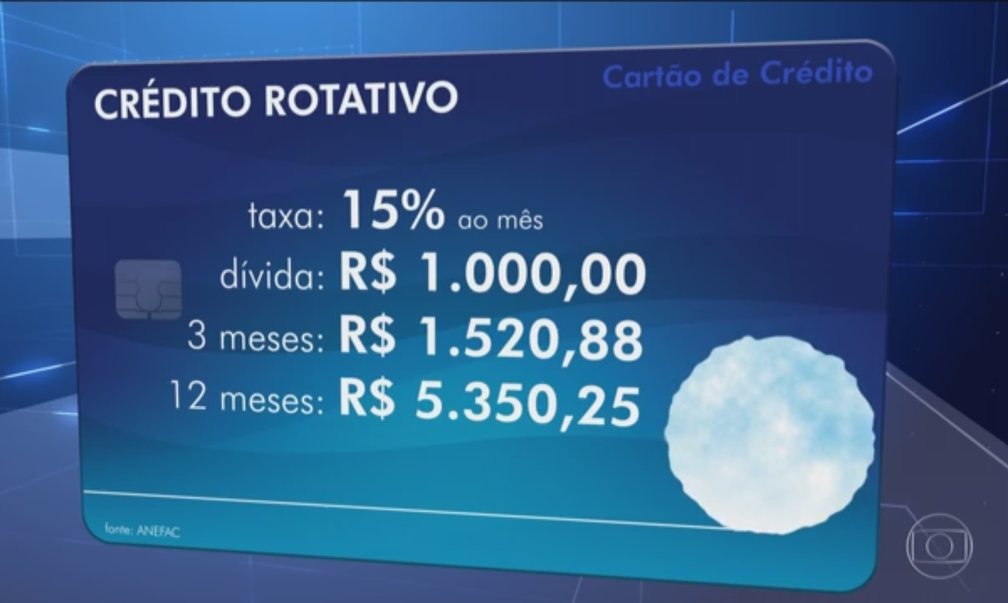
\includegraphics[width=0.4\textwidth]{credito-rotativo-1}\hspace{1em}
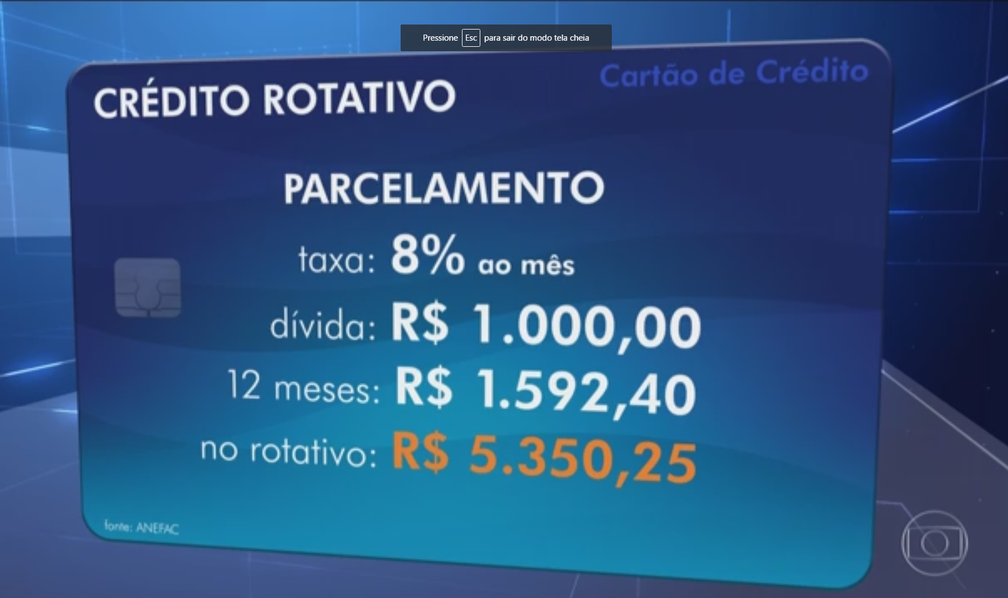
\includegraphics[width=0.4\textwidth]{credito-rotativo-2}
\justify

Por que as pessoas usam o cartão de crédito para tomar dinheiro emprestado?
\end{reflection}

Generalizando, uma quantia $\mathit{VP}$, aplicada a uma taxa $i$ por período, transforma-se após $n$ períodos, em um valor futuro $\mathit{VF}$ igual a:

$$\mathit{VF}=\mathit{VP}\cdot(1+i)^n $$ 

Isso acontece pois se a cada período, o valor futuro do período anterior é multiplicado por $(1+i)$, então após $n$ períodos, teremos que o $\mathit{VP}$  ficará multiplicado pelo fator $(1+i)$ $n$ vezes, gerando o Valor Futuro $\mathit{VF}$. Podemos então escrever que: $\mathit{VF}=\mathit{VP}\cdot(1+i)^n$. 

Vimos aqui mais uma causa da transformação do dinheiro no tempo: os juros, que são uma forma de aluguel do dinheiro. \textbf{Quem paga juros, opta por uma troca intertemporal: usufruir do dinheiro de terceiros hoje, ou por um período, e pagar ao longo do tempo o que pegou acrescido de uma quantia adicional, chamada juro.}

A situação referente ao investimento de Humberto é uma troca intertemporal, pois ele optou em abrir mão de um dinheiro hoje (fazer um sacrifício hoje, ao investir) para obter um benefício no futuro – um valor acrescido de juros, para atingir algum objetivo específico, dentre eles proteção do dinheiro, poupança, férias, viagem, doação, criar um projeto social, trocar de carro, dentre muitos outros. 

Na \textbf{segunda atividade} temos duas situações envolvendo o aumento de preços produzido pela alta do dólar. Uma foi no preço do pão; a outra no preço de produtos eletrônicos. Mas por que isso acontece?

Isso acontece porque vários produtos, dentre eles a farinha de trigo para a produção do pão, e dos componentes eletrônicos no caso de produtos eletroeletrônicos (celulares, smartphones, televisores, caixas de som, geladeiras, computadores, tablets, fones, dentre outros) têm seus preços atrelados ao dólar. As empresas nos vendem os produtos em reais, mas compram trigo e eletrônicos dos fornecedores pagando em dólares. E a quantidade de reais necessários para comprar um dólar pode variar no tempo. Eis o dinheiro se transformando no tempo, e isso não tem nada a ver com juros.

Por exemplo, se 1 dólar custava 4 reais em janeiro e 5 reais em maio, isso significa que os preços em reais provavelmente vão mudar. Para comprar um produto que custava 1000 dólares no primeiro semestre de 2020, a empresa compradora precisará de 4.000 reais em janeiro e de 5.000 reais em maio. Observe que o preço de 1.000 dólares não mudou, mas em reais o preço aumentou.

Olhando para a variação de reais gastos, de $4.000$ para $5.000$ reais, os preços em reais aumentaram:
\begin{equation*}
\frac{(5.000-4.000)}{4.000}=25\%
\end{equation*}

Por outro lado, o valor do real diminui em $20$\%, pois um real valia $\frac{1}{4}=0{,}25$ dólares, e passou a valer $\frac{1}{5}=0{,}20$ dólares, logo o valor do real variou de 
\begin{equation*}
\frac{(0{,}20-0{,}25)}{0{,}25}=-20\%
\end{equation*}

Nesse caso, os preços em reais aumentaram em $25$\%, e o real se desvalorizou em $20$\%, por isso a taxa é negativa.

Ou seja, a variação cambial produziu uma transformação no valor do dinheiro no tempo. Isso aconteceu, por exemplo, no primeiro semestre de 2020 no Brasil, onde vivenciamos uma forte alta do dólar dólar com a pandemia do novo coronavírus, que influenciou o aumento de preço em vários produtos, dentre eles os eletrônicos.

\begin{observation}
{Você tem percebido o impacto da variação cambial na sua vida e de sua família?}
\end{observation}

Na \textbf{terceira atividade} temos um exemplo de uma transformação do dinheiro no tempo diferente das duas apresentadas anteriormente.

O valor da conta não muda até a data do vencimento, nesse caso, pois não há informações sobre algum tipo de desconto para quem pagar antes do vencimento.

Entretanto, depois do vencimento, o valor da conta muda com o tempo. Mas a forma de cálculo é diferente das duas situações anteriores. Veja a imagem do boleto.

\begin{figure}[H]
\centering

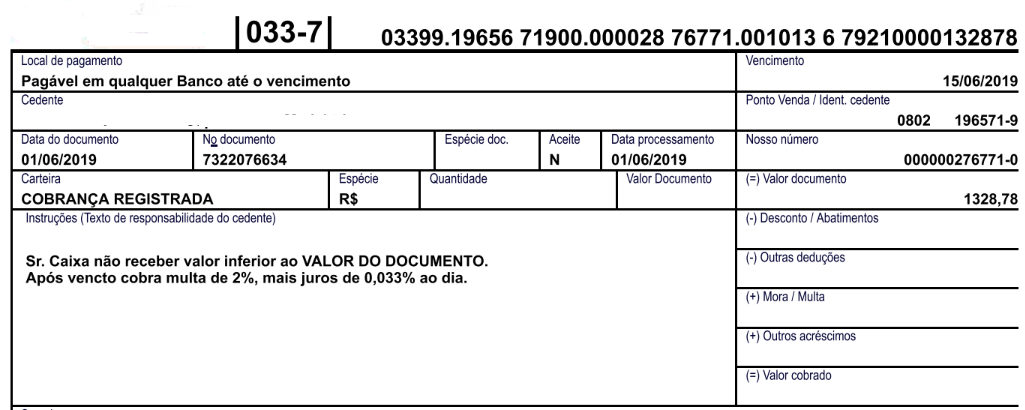
\includegraphics[width=425bp]{financeira7}
\end{figure}

Há cobrança de uma multa de $2$\%, aplicada sobre o valor da conta até o vencimento, e mais juros de $0{,}033$\% ao dia. Esses juros são chamados de juros simples, pois a taxa incide sobre o valor inicial, e não sobre o valor acumulado da dívida. Os juros simples são diretamente proporcionais ao tempo e à taxa, referidos a uma mesma unidade.

Assim, como José pagou a conta com 6 dias de atraso, pois o vencimento era 15/06/2019 e ele pagou no dia 21/06/2019, ele pagará juros de $0{,}033$\% sobre o valor da conta, por cada dia de atraso. Assim, ele vai pagar $6\times0{,}033$\% sobre o valor da conta, gerando juros de R\$ $2{,}36$.

Matematicamente, podemos calcular assim:
\begin{align*}
J&=\text{R\$ }1.328{,}78\times0{,}033\%/\text{dia}\times6\text{ dias}\\
J&=\text{R\$ }2{,}36
\end{align*}

Além disso, há uma multa de $2$\% sobre o valor da conta.
\begin{align*}
\text{Multa}&=\text{R\$ }1.328{,}78\times2\%\\
\text{Multa}&=\text{R\$ }26{,}58
\end{align*}

De uma maneira geral, no sistema de juros simples, com taxa i ao período, os juros diretamente proporcionais ao tempo e à taxa variam, período a período, da seguinte forma: 
\begin{align*}
\text{Após 1 período, temos } J&=i\cdot \mathit{VP} \\
\text{Após 2 períodos, temos } J&=2i\cdot \mathit{VP} \\
\text{Após 2 períodos, temos } J&=3i\cdot \mathit{VP} \\ 
\end{align*}
Mantendo o padrão, temos:
\begin{equation*}
\text{Após $n$ períodos, temos } J=ni\cdot \mathit{VP} \\ 
\end{equation*}
Assim, a sequência formada pelos juros é uma progressão aritmética.

Assim, após $n$ períodos aumentando de uma taxa $i$ a cada período, o valor presente, nesse sistema de juros simples, vai se transformar em $\mathit{VP}+ni\cdot\mathit{VP}$ e, portanto, o valor futuro será igual a:
{\Large
\begin{equation*}
\mathit{VF} = \mathit{VP}(1 + ni)
\end{equation*}}
Ou seja, o $\mathit{VF}$, no regime de juros simples, cresce segundo uma progressão aritmética de termo inicial $\mathit{VP}$ e razão igual a $\mathit{VP}\cdot i$ (juros de cada período unitário)

Vimos assim alguns fatores que influenciam o valor do dinheiro no tempo. Para sabermos a forma de transformação do dinheiro no tempo, e os cálculos que vamos utilizar, precisamos saber qual é a regra que está sendo usada. Vimos que juros compostos funcionam de uma maneira, juros simples de outra e a variação cambial de outra.

Um valor presente se transformando em um valor futuro, ou seja, em cada situação tínhamos apenas a transformação de uma quantia ao longo do tempo. Veremos na próxima seção que podemos ter um ou mais capitais se transformando em um ou mais capitais ao longo do tempo.

\begin{reflection}
As pessoas atribuem valor às coisas tendo ou não consciência disso. E esse valor influencia profundamente as decisões humanas, impactando fortemente o curso da história. Talvez por isso a tomada de decisão humana vem sendo estudada por diferentes áreas, dentre elas a sociologia, a antropologia, a psicologia, a economia, o marketing, dentre outras.

Quando falamos de valor do dinheiro no tempo, estamos discutindo apenas uma visão, dentre muitas, sobre qual é o valor que o dinheiro realmente possui. E mesmo assim, muitas interpretações podem surgir.


Por exemplo, qual o valor de uma cesta básica de 150 reais para uma família carente e para uma família abastada? $1.000$ reais para um jovem da perifeira no início de carreira tem o mesmo valor que $1.000$ reais para um jovem rico? O que tem mais valor: possuir uma casa própria e ficar pagando 30 anos, ou morar de aluguel e usar o dinheiro dos juros para pagar o aluguel e com a sobra viajar e conhecer diversos lugares no mundo?

O que pode ter muito valor para você, pode não ter para o seu irmão e amigo. O que pode ter muito valor para você hoje, pode não ter para você daqui a 15 anos. O que pode ter pouco valor para a sociedade hoje, pode ter muito valor em alguns meses no futuro. Por exemplo, qual o valor que a sociedade brasileira dava ao álcool em gel em janeiro de 2020? E em abril de 2020?
\clearpage

\begin{wrapfigure}[12]{r}{.275\textwidth}
\vspace{-1.1em}
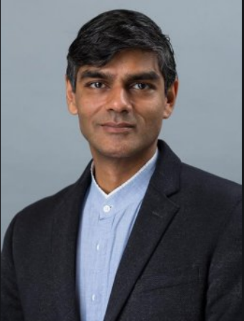
\includegraphics[width=.275\textwidth]{financeira8}
\end{wrapfigure}
Haj Patel, economista e professor da universidade de Berkeley, nos diz que vivemos uma era em que é muito comum associar a ideia de "valor das coisas"{} ao preço que elas custam. Para ele, um dos problemas dessa associação entre valor e preço é o fato de que o preço pode ser distorcido e o valor também. O valor da etiqueta não se resume ao custo de produção somado à margem de lucro. Custos ambientais (emissão de CO$_{\text{2}}$, poluição de rios, degradação da terra na extração de minerais), de saúde (alimentos associados a cardiopatias e obesidade), e sociais (trabalho escravo, subempregos, geração de conflitos locais) estão embutidos no preço dos produtos.

Além disso, frases como: se é caro deve ser bom, ou ainda, tem que custar caro porque é muito bom, fazem parte da opinião de muita gente que conhecemos, e são bem frequentes na sociedade predominantemente capitalista que experimentamos. Como Oscar Wilde escreveu a mais de um século: "hoje em dia, as pessoas sabem o preço de tudo e o valor de nada".

De uma maneira geral, podemos tentar entender o valor como um parâmetro que usamos para avaliar a capacidade de algo satisfazer nossas necessidades e do grupo social em que vivemos. Refletir sobre qual valor atribuímos a bens, serviços, atitudes, comportamentos, ideias é muito importante, pois as consequências das nossas escolhas baseadas no valor que damos às coisas podem ser geradoras de vida e paz ou produtoras de morte e guerra.
\end{reflection}

\clearpage

\def\currentcolor{session2}

\begin{objectives}{O rapaz que editava vídeos}
{
\begin{itemize}
\item Identificar diferentes fatores que influenciam o valor do dinheiro no tempo, tais como juros, inflação, câmbio, investimentos e percepção de utilidade
\item Resolver problemas relacionados a Valor Presente e Valor Futuro no regime de juros simples ou compostos.
\item Analisar e tomar decisões em situações econômico-financeiras que envolvam o valor do dinheiro no tempo, considerando aspectos matemáticos e não matemáticos.
\end{itemize}
}{1}{1}
\end{objectives}

\begin{sugestions}{O rapaz que editava vídeos}
{
Nessa atividade convidamos o estudante a pensar uma situação que envolve escolhas já feitas pelo personagem e escolhas que serão feitas pela personagem. A pergunta do item a é pessoal e tem como objetivo levantar a discussão sobre o que é ótimo financeiro e o ótimo pessoal. O que pode ser melhor para uma pessoa, pode ser péssimo para outra. Trazemos também uma discussão sobre a cobrança de imposto em algumas aplicações financeiras.

Chamamos a atenção para o fato de que é apesar do sistema de juros compostos ser o praticado nas duas situações, a forma como intencionalmente desenhamos a atividade faz com que isso seja desnecessário nessa situação. O importante aqui não está na forma dos juros, mas no tipo de aplicação, a incidência do tributo, o efeito disso no lucro, e de como isso é levado em consideração para tomar decisão.

Recomendamos que o professor amplie a parte das questões abertas, discutindo o que eles fariam com os $2.000$ reais se estivessem no lugar do Fábio.
}{1}{1}
\end{sugestions}
\begin{answer}{O rapaz que editava vídeos}
{
  \begin{enumerate}
    \item Resposta pessoal
    \item O valor futuro líquido da poupança seria R\$ $1040{,}00$ e da aplicação do tesouro direto seria de R\$ $1048{,}00$.

    \item Veja que a primeira opção, se Fábio deixar o valor de R\$ $1.000{,}00$ com os pais dele, este dinheiro não lhe renderá juros ao final de um ano. Na segunda opçãso, se Fábio aplicar o seu dinheiro na poupança durante 12 meses (1 ano) a uma taxa de $4$\%, ao final de um ano, Fábio terá o montante de R\$ $1.040{,}00$. Na terceira opção, se Fábio aplicar o dinheiro no tesouro direto, ao final de um ano, ele terá a quantia de R\$ $1.060{,}00-12{,}00$ ($20$\% de R\$ $60{,}00$)$=$R\$ $1.048{,}00$. Logo, a melhor opção seria ele aplicar R\$ $1.000{,}00$ no tesouro direto, pois é a aplicação com maior rentabilidade.

    A opção que produz maior ganho financeiro é o tesouro direto, como é possível observar na solução da letra \titem{a)}.
  \end{enumerate}
}{0}
\end{answer}
\clearmargin
\begin{objectives}{O valor do amanhã}
{
\begin{itemize}
\item Identificar diferentes fatores que influenciam o valor do dinheiro no tempo, tais como juros e investimentos.
\item Resolver problemas relacionados a Valor Presente e Valor Futuro no regime de juros simples ou compostos.
\item Analisar e tomar decisões em situações econômico-financeiras que envolvam o valor do dinheiro no tempo, considerando aspectos matemáticos e não matemáticos.
\end{itemize}
}{1}{2}
\end{objectives}
\begin{sugestions}{O valor do amanhã}
{
Nessa atividade convidamos o estudante a continuar pensando nas decisões de investimento de Fábio, trazendo um contexto com opções de investimento, ampliando-se os prazos nos quais o dinheiro ficará investido, e aumentando o número de opções de investimento.
Buscamos aqui usar o simulador do site do Tesouro Direto. E isso tem duas implicações. O professor pode usar a própria atividade já pronta, ou criar sua própria atividade usando o simulador no próprio site, ou convidar os alunos a fazerem suas próprias simulações e investigarem seus próprios resultados.
Na atividade, não queremos sobrecarregar os alunos com contas, mas convidá-los a experimentar, simular e investigar as diferentes modalidades, percebendo as diferenças entre elas.
Essa atividade tem forte potencial para desenvolver a habilidade da BNCC (\textbf{EM13MAT203}): aplicar conceitos matemáticos no planejamento, na execução e na análise de ações envolvendo a utilização de aplicativos e a criação de planilhas (para o controle de orçamento familiar, simuladores de cálculos de juros simples e compostos, entre outros), para tomar decisões.

}{1}{2}
\end{sugestions}
\begin{answer}{O valor do amanhã}
{
  \begin{enumerate}
    \item O Tesouro é a aplicação que apresenta maior valor líquido de resgate e a maior rentabilidade líquida, portanto, seria a melhor opção para investir.
    \item A vantagem da Poupança em relação ao Tesouro é que a Poupánça tem custo e valor de imposto de renda zero. A desvantagem é que a Poupança rende menos que o Tesouro.

    No tesouro, é importante levar o investimento até a data do vencimento. Apesar do investidor poder resgatar a qualquer momento, variações no preço dos títulos decorrentes de fatores econômicos variados, podem reduzir o retorno prometido, incluindo até mesmo trazer prejuízo a quem resgata antes, como também pode ampliar o retorno prometido em alguns casos, como por exemplo, em contexto de redução de taxa Selic. 
  \end{enumerate}
}{0}
\end{answer}
\clearmargin
\begin{objectives}{Tomando decisões diante das emergências}
{
\begin{itemize}
\item Identificar diferentes fatores que influenciam o valor do dinheiro no tempo, tais como juros e investimentos.
\item Resolver problemas relacionados a Valor Presente e Valor Futuro no regime de juros simples ou compostos.
\item Analisar e tomar decisões em situações econômico-financeiras que envolvam o valor do dinheiro no tempo, considerando aspectos matemáticos e não matemáticos.
\end{itemize}
}{1}{1}
\end{objectives}
\begin{sugestions}{Tomando decisões diante das emergências}
{
Nessa atividade convidamos o estudante a analisar uma SEF envolvendo uma emergência que demanda uma tomada de decisão entre tirar o dinheiro na poupança para atender a emergência ou deixar o dinheiro na poupança e pedir dinheiro emprestado ao Banco, usando uma modalidade chamada Cheque Especial.

Aqui, o estudante vai precisar efetuar os cálculos do Valor Futuro, usando os modelos exponenciais adequados para isso. Recomendamos o uso de calculadora científica (também disponível para baixar nos smartphones e tablets). 

Buscamos também convidar os alunos a compararem diferentes custos bancários, por meio da leitura da tabela e da simulação de diferentes taxas.

Finalmente, levamos em consideração o custo de oportunidade de Vanessa, ou seja, quanto ela deixaria de ganhar ao retirar o dinheiro da poupança, para uma análise mais completa da situação. 

}{1}{1}
\end{sugestions}
\begin{answer}{Tomando decisões diante das emergências}
{
  \begin{enumerate}
    \item A estratégia menos custosa para Vanessa seria utilizar o dinheiro da poupança, pois ela não teria que pagar os juros de empréstimo para nenhum banco.
    \item Durante três meses, Vanessa 

    \begin{itemize}
      \item teria um valor, a uma taxa mensal de $0{,}5$\% na poupança, de $10{,}000\times(1+0{,}005)^3) = 10.150{,}75$, ou seja, deixaria de ganhar R\$ $150{,}75$ reais;
      \item pagaria na Caixa Econômica Federal, a uma taxa mesal de $5{,}20\%$, o valor de $10.000\times(1+0{,}052)^3=11.642{,}53$ reais;
      \item pagara No Banco do Brasil S.A., a uma taxa de mensal de $7{,}57$\%, o valor total de $10{,}000\times(1+0{,}0757)^3=12.447{,}25$;
      \item pagaria no banco Itaú, a uma taxa de $7{,}70$\% ao mês, $10.000\times(1+0{,}077)^3=12.492{,}43$ reais;
      \item pagaria banco Bradesco S.A., a uma taxa mensal de $7{,}63$\%, o valor total de $10.000\times(1+0{,}0763)^3=12.468{,}09$.
    \end{itemize}
  \end{enumerate}
}{0}
\end{answer}

\practice{Valor Presente e Valor Futuro}
\label{fin-prac-3}

\begin{task}{O rapaz que editava vídeos}
\label{fin-ativ-15}

Fábio é um rapaz apaixonado por futebol, e tem se aperfeiçoado em editar vídeos. Mesmo tendo apenas 16 anos, ele ajuda seu pai e sua mãe na venda de bolos e doces pela internet. Para conciliar essas duas atividades com suas aulas na escola pela manhã, com curso de inglês à tarde e com o futebol dos amigos nos finais de semana, ele precisa de planejamento e disciplina. Um dos frutos de tudo isso é que ao longo desse ano ele conseguiu juntar uma quantia de R\$ $2.000{,}00$. Ele decidiu gastar R\$ $1.000{,}00$ com ele, comprando roupas e fazer um novo surso sobre artes digitais roupas digitais e fazendo um novo curso sobre artes digitais, e guardar os outros R\$ $1.000{,}00$. Mas onde vai guardar esse dinheiro? Ele considera três opções:
\begin{itemize}
  \item deixar o dinheiro com os pais dele, e pegar quando percisar;
  \item aplicar o dinheiro na poupança;
  \item aplicar o dinheiro no tesouro direto, usando a conta da mãe.
\end{itemize}

Considere que, durante os 12 meses seguintes, a aplicação de Fábio na poupança remunere a uma taxa de $4$\% ao ano, sem cobrança de impostos, e o tesouro direto a $6$\% ano ano, com a cobrança de $20$\% de IR (imposto de renda) sobre os juros pagos.

\begin{enumerate}
  \item Qual das três opções você escolheria?
  \item Qual o valor futuro líquido (retirados os impostos) de cada uma das aplicações?
  \item Qual das três opções produz o maior ganho financeiro?
\end{enumerate}
\end{task}

\clearpage
\begin{task}{O valor do amanhã}
\label{fin-ativ-16}

Pensando no longo prazo, Fabio fez uma simulação em outro título, investindo os 1.000 reais em 01/ago/2020, e retirando o acumulado na data do vencimento em 01/ja/2026. O resultado da simulação está apresentado a seguir, onde os investimentos simulados no primeiro quadro estão representados no gráfico a seguir.

\begin{figure}[H]
\centering

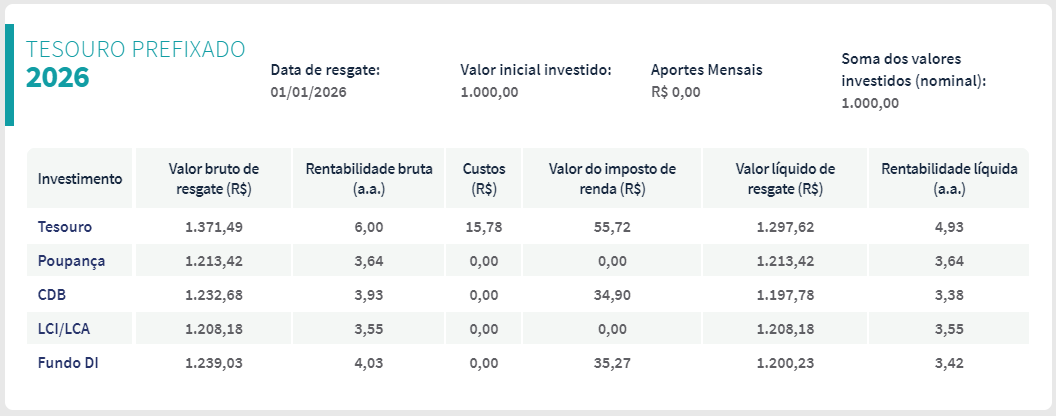
\includegraphics[width=450bp]{financeira9}

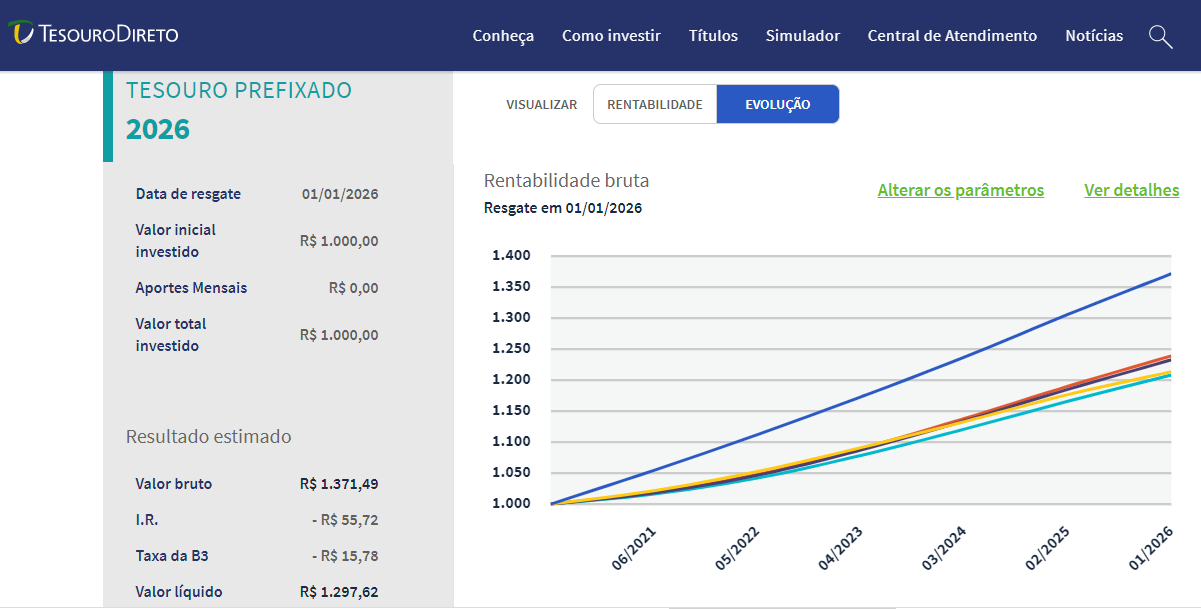
\includegraphics[width=450bp]{financeira10}
\end{figure}

Olhando para as simulações, responda:
\begin{enumerate}
  \item Em qual das cinco opções você investiria o dinheiro? Justifique sua resposta usando tanto a tabela quanto o gráfico.
  \item Quais são as vantagens e desvantagens da poupança em relação ao título do tesouro direto apresentado na simulação?
\end{enumerate}
\end{task}


\begin{task}{Tomando decisões diante das emergências}
\label{fin-ativ-17}

Vanessa teve uma emergência e precisa de $10.000$ reais para daqui a dois dias. Ela pode usar o cheque especial para fazer um empréstimo pelo bankline, ou buscar uma alternativa mais barata. Pensando um pouco, ela lembra que tem $10.000$ reais na poupança, guardados por ela mesmo para alguma emergência. Considere que esse dinheiro na poupança renda $0{,}5$\% ao mês para Vanessa, enquanto que as taxas do cheque especial cobradas pelos principais bancos brasileiros estão apresentadas no quadro a seguir. Ela precisa decidir se tira o dinheiro da poupança ou se pega dinheiro com o banco usando o cheque especial.

\begin{table}[H]
\centering

\begin{tabular}{|l|c|r|}
\hline
\tcolor{Banco} & \tcolor{Taxa Mensal (\%)} & \tcolor{Taxa Anual (\%)} \\
\hline
BCO BMG S.A. & 3{,}00 & 42,58 \\
\hline
BANCO MODAL & 3,68 & 54,31 \\
\hline
BCO FATOR & 4{,}00 & 60,10 \\
\hline
BCO DO NORDESTE DO BRASIL & 4,71 & 73,66 \\
\hline
CAIXA ECONOMICA FEDERAL & 5,20 & 83,70 \\
\hline
BCO DO BRASIL S.A. & 7,57 & 140,02\\
\hline
BCO BRADESCO S.A. & 7,63 & 141,68 \\
\hline
ITAÚ UNIBANCO S.A. & 7,70 & 143,57 \\
\hline
BANCO ORIGINAL & 7,80 & 146,20 \\
\hline
BCO SAFRA S.A. & 7,84 & 147,32 \\
\hline
BCO SANTANDER (BRASIL) S.A. & 7,95 & 150,36 \\
\hline
\end{tabular}
\caption{Fonte: Banco Central. Período de julho/2020}
\end{table}




\begin{enumerate}
  \item Qual a estratégia menos custosa para Vanessa, dentre as duas apresentadas, do ponto de vista exclusivamente financeiro, independente de qual Banco ela seja cliente? Justifique sua resposta.
  \item Quantos reais ela economizaria em juros, considerando as duas opções, ou seja, comparando o que ela vai pagar de juros no cheque especial com o que ela vai deixar de ganhar na poupança, para um empréstimo de 10.000 reais durante 3 meses? Considere aqui os dois maiores bancos públicos e os dois maiores privados do Brasil.
\end{enumerate}
\end{task}


\begin{paginatexto}{O valor do dinheiro no tempo: capitais equivalentes}

\subsection*{Objetivos gerais}

\begin{itemize}
\item Investigar situações financeiras que envolvem o valor do dinheiro no tempo, considerando o conceito de capitais equivalentes 
\item Resolver problemas relacionados aos capitais equivalentes.
\item Analisar e tomar decisões em situações econômico-financeiras que envolvam o conceito de capitais equivalentes, considerando aspectos matemáticos e não matemáticos.

\item \textbf{Conceitos abordados: taxas, fatores e capitais equivalentes.}
\end{itemize}


Investigar situações financeiras que envolvem o valor do dinheiro no tempo, considerando o conceito de capitais equivalentes, através das habilidades:

\begin{habilities}{EM13MAT101}
 Interpretar situações econômicas, sociais e das Ciências da Natureza
que envolvem a variação de duas grandezas, pela análise dos gráficos das funções representadas e das taxas de variação com ou sem apoio de tecnologias digitais.

\tcbsubtitle{EM13MAT203}
Planejar e executar ações envolvendo a criação e a utilização de aplicativos, jogos (digitais ou não), planilhas para o controle de orçamento familiar, simuladores de cálculos de juros compostos, dentre outros, para aplicar conceitos matemáticos e tomar decisões. 

\tcbsubtitle{EM13MAT507}
Identificar e associar sequências numéricas (PA) a funções afins de domínios discretos para análise de propriedades, incluindo dedução de algumas fórmulas e resolução de problemas.

\tcbsubtitle{EM13MAT508}
Identificar e associar sequências numéricas (PG) a funções exponenciais de domínios discretos para análise de propriedades, incluindo dedução de algumas fórmulas e resolução de problemas.
\end{habilities}

\subsection*{Recomendações para o professor}

\paragraph{Organização em sala de aula} Essa seção pode ser vista como uma extensão da anterior. Vamos investigar situações financeiras em que podemos ter um ou mais capitais se transformando em um ou mais capitais ao longo do tempo. A primeira atividade aponta para isso, e pode ser ralizada em grupos de quatro alunos, geranto interação entre os estudantes e identificação com os personagens da atividade. Convide seus alunos a criar a cultura de investigar os fundamentos e razoabilidade das informações veiculadas nas mídias sociais de forma fundamentada.

\paragraph{Dificuldades previstas} Os cálculos agora são um pouco mais complexos, e podem demandar maior manipulaçõa algébrica enolvendo equações fracionárias. Começar de exemplos com poucos valores, e estruturar o problema usando a representação temporal que privilegia o presente para o futuro para o futuro pode ajudar na abordagem do tema.

\paragraph{Sugestões gerais}
Falar sobre capitais equivalentes é falar sobre trocas intertemporais, tendo ou não consciência disso. Reforçamos que nessa seção vamos investigar situações em que podemos ter um ou mais capitais se transformando em um ou mais capitais ao longo do tempo.

Primeira sugestão: Ir do presente para o futuro é mais intuitivo e costuma ser melhor recebido pelos alunos segundo algumas pesquisas, tais como \cite{campos2013}, \cite{muniz2016b}, \cite{santana2019}. Então sugerimos fortemente iniciar com abordagens em que o dinheiro se transforme do presente para o futuro. A seções organizando mostra de, de forma bem clara, um exemplo disso. Comparar os valores em cada data, ainda que se faça isso mais de uma vez, costuma ser melhor, segundo os estudos de \citeauthor{muniz2016a} (\citeyear{muniz2016b}), do que simplesmente trazer todos os valores do futuro para o presente. Entenda bem, sinda que a equivalência de capitais nos forneça que não importa a data de comparação de capitais, o que importa é que seja a mesma. Trabalhar representações do presente para o futuro se alinha com a nossa percepção de tempo, e isso costuma ser muito bem recebido e utilizado pelos alunos.

\subsection*{Enriquecimento da discussão}

Para abordar capitais equivalentes, sugerimos fortemente a leitura completa de dois artigos, sendo o primeiro sobre a noção de trocas temporais e o segundo sobre o conceito de representações temporais. Cuidado, pois são coisas bem diferentes, ainda que o conceito de representação temporal tenha sido criado pelo autor, em sua tese de doutorado, para a descrição e abordagem didática de situações financeiras envolvendo trocas intertemporais.

\begin{enumerate}
  \item \textit{Tomada de decisão e trocas intertemporais: uma contribuição para a construção de ambientes de educação financeira escolar nas aulas de matemática. \citep{muniz2016c}.}

  \item \textit{Representações temporais e o valor do dinheiro no tempo: conexões entre Educação financeira eo ensino de Matemática.}
\end{enumerate}

Do nosso primeiro artigo, destacamos os sete papéis das trocas intertemporais. Diante desses exemplos, e de tantos outros que poderíamos apresentar, os papéis das trocas intertemporais podem ser sintetizados em sete pontos nodais:
\begin{enumerate}
  \item permitem discutir a transformação/valor do dinheiro no tempo, uma questão central em nossa concepção de EFE;
  \item contribuem para a reflexão sobre os fatores que geram a mudança do valor do dinheiro no tempo, tais como juros, inflação, desvalorização cambial, oporturidades de investimento, renda e emprego.
  \item caracterizam um incontável número de situações econômico-financeiras, que envolvem sacrifícios e benefícios que acontecem em diferentes momentos do tempo;
  \item permitem tratar de questões sociais, éticas e ambientais, dentro da perspectiva das trocas que as pessoas fazem ao longo de suas vidas e uas possíveis consequências;
  \item convida para a reflexão sobre os efeitos do planejamento de curto, médio e longo prazo na realização de sonhos e na proteção contra injustiças, desigualdades e armadilhas;
  \item estimula a discussão sobre questões comportamentais, tais como impaciência, cultura do consumo, viver o agora antes que acabe, mudança de perfil de consumo, dentre outras;
  \item Contribui para a discussão sobre aspectos macroenconômicos, como inflação, política de câmbio e geração de renda, relacionados às possibilidades e limitações nas e das tomadas decisões indivicuais, familiares e de uma sociedade.
\end{enumerate}
  Do nosso segundo artigo, convidamos o proessor a ampliar a visão sobre as representações temporais, isto é, representações de situações financeiras envolvendo a transformação do dinheiro no tempo. Os esquemas com eixos de setas, seta para cima, seta para baixo, são apenas algumas das formas de se representar trocas intertemporais e os valores em suas respectivas datas.

  Para esse convite, destacamos o seguinte trecho do artigo de \cite[p. 125]{muniz2016b}.

  Chamamos de \textit{Representações Temporais} as representações pictóricas (gráficas, tabulares ou esquemáticas) que permitem:
  \begin{enumerate}
    \item associar as quantias às suas respectivas datas;
    \item reforçar o dinamismo do valor do dinheiro no tempo;
    \item auxiliar na análise da evolução de dívidas e/ou saldos acumulados;
    \item auxiliar na determinação do tempo de transformação de uma quantia ou de uma série de quantias;
    \item contribuir parar explorar a equivalência de capitais, a partir das taxas de desconto ou de retorno fornecidas ou procuradas.
  \end{enumerate}

Tais representações têm se mostrado importantes para os alunos na análise de variadas situações, como apontam nossos resultados iniciais, principalmente quando voltamos nosso foco para questões relativas ao ensino e investigação, pois contribuem, além do que já expomos, para ampliar ainda mais as possibilidades de se mostrar que o valor do dinheiro, dada uma taxa, muda com o tempo, e os impactos disso na vida das pessoas.

No livro aberto de Educação Financeira, utilizamos representações temporais variadas, e não apenas o eixo das setas apresentado no excelente livro Progressões e Matemática Financeira do amigo e eterno professor Morgado.
\end{paginatexto}
\clearpage

\def\currentcolor{session1}
\begin{objectives}{E o tempo levou!}
{
\begin{itemize}
\item Investigar situações financeiras que envolvem o valor do dinheiro no tempo, considerando o conceito de capitais equivalentes 
\item Resolver problemas relacionados aos capitais equivalentes.
\item Analisar e tomar decisões em situações econômico-financeiras que envolvam o conceito de capitais equivalentes, considerando aspectos matemáticos e não matemáticos.
\end{itemize}
}{1}{1}
\end{objectives}
\begin{sugestions}{E o tempo levou!}
{
Nessa atividade disparadora da seção sobre equivalência de capitais convidamos o estudante a analisar uma SEF envolvendo quatro jovens que aplicaram uma mesma quantia (300 reais), a uma mesma taxa, só que distribuídos de diferentes formas ao longo do tempo, como estratégias de poupança para a festa de formatura no final do ano. 

Queremos convidar o estudante a perceber como prazo de aplicação, o valor aplicado, e o momento da aplicação influenciam no valor futuro, bem como ensinar com a matemática ajuda a modelar a situação. Os quatro investiram o mesmo valor (nominal), mas não terão o mesmo valor ao final da operação.
Reforçamos que dois ou mais capitais são equivalentes, a uma mesma taxa, quanto têm o mesmo valor quando comparados em uma mesma data. É esse conceito que vamos explorar nessa seção.

}{1}{1}
\end{sugestions}
\begin{answer}{E o tempo levou!}
{
A Atividade será detalhadamente investigada no próximo organizando as ideias.
}{1}
\end{answer}
\explore{Capitais Equivalentes}
\label{fin-exp-4}

Nas situações anteriores, tínhamos uma quantia se transformando em outra ao longo do tempo, ou seja, um valor presente se transformando em um valor futuro. Convidamos você a investigar e refletir com a gente situações em que podemos ter um ou mais capitais se transformando em um ou mais capitais ao longo do tempo.



\begin{task}{e o tempo levou!}
\label{fin-ativ-18}

Considere que quatro estuandtes da última série do Ensino Médio combinaram poupar trezentos reais cada um para comprarem um presente de formatura no final de 2019. As estratégias de poupança usadas por eles foram todas diferentes entre si, conforme mostra o quadro a seguir.

\begin{table}[H]
\centering

\begin{tabular}{|l|*{6}{c|}}
\hline
\tcolor{} & \tcolor{jul/19} & \tcolor{ago/19} & \tcolor{set/19} & \tcolor{out/19} & \tcolor{nov/19} & \tcolor{dez/19} \\
\hline
{Giovana} & $100$ & $100$ & $100$ & & & \\
\hline
{Polyana} & $300$ & & & & & \\
\hline
{Juliana} & $150$ & $150$ & & & & \\
\hline
{Luiz Felipe} & & & $300$ & & & \\
\hline
\end{tabular}
\end{table}

\begin{enumerate}
  \item Qual a estratégia mais viável financeira para você?
  \item Sem fazer as contas, qual estratégia lhe parece gerar o maior valor acumulado ao final?
  \item Considerando que todos eles consigam fazer o dinheiro render a uma taxa de 1\% ao mês, quem vai obter o maior valor acumulado em dez/19? Justifique apresentando as contas.
  \item Compare a sua resposta no item \textcolor{\currentcolor}{\textbf{b)}} com a do item \textcolor{\currentcolor}{\textbf{c)}}. Caso tenham sido diferentes, por que você acha que isso aconteceu?
\end{enumerate}
\end{task}

\arrange{Capitais Equivalentes}
\label{fin-arg-4}

Vamos analisar a transformação do dinheiro no tempo para cada um dos quatro estudantes. 

Primeiro, vamos investigar como os valores aplicados pelos quatro estudantes se transformam ao longo do tempo. Comecemos pela estratégia de Giovana.
\begin{table}[H]
\centering
\begin{tabular} {|c|c|c|c|c|c|}
\hline
\tmcol{6}{|c|}{Giovana}\\
\hline
jul/19 & ago/19 & set/19 & out/19 & nov/19 & dez/19 \\
\hline
100\tikzmark{a1} & & & & & \tikzmark{b1}\\
\hline
& 100\tikzmark{c1} & & & & \tikzmark{d1}\\
\hline 
& & 100\tikzmark{e1} & & & \tikzmark{f1}\\
 \hline
\end{tabular}
\begin{tikzpicture}[overlay, remember picture, shorten >=5pt, shorten <=5pt, ,transform canvas={yshift=.13cm}]

\draw [->, very thick, \currentcolor] ({pic cs:a1}) to ({pic cs:b1});
\draw [->, very thick, \currentcolor] ({pic cs:c1}) to ({pic cs:d1});
\draw [->, very thick, \currentcolor] ({pic cs:e1}) to ({pic cs:f1});

\end{tikzpicture}
\end{table}


\begin{table}[H]
\centering
\begin{tabular} {|c|c|c|c|c|c|}
\hline
\tmcol{6}{|c|}{Giovana}\\
\hline
Jul/19 & Ago/19 & Set/19 & Out/19 & Nov/19 & Dez/19 \\
\hline
R\$ 100  & R\$ 101{,}00 & R\$ 102,01 & R\$ 103,03 & R\$ 104,06 & R\$ 105,10 \\
\hline
& R\$ 100 & R\$ 101{,}00 & R\$ 102,01 & R\$ 103,03 & R\$ 104,06  \\
\hline 
& & R\$ 100 & R\$ 101{,}00 & R\$ 102,01 & R\$ 103,03  \\
\hline
& & & & \tmcol{1}{|c|}{Total =} & \tmcol{1}{|c|}{R\$ 312,19} \\
\hline
\end{tabular}
\end{table}
Na representação temporal acima, observe que os 100 reais aplicados em jul/19 transformam-se em 101 reais em ago/19, depois em 102,01 em set/19, em seguida em 103,03 em out/19, em 104,06 em nov/19 e finalmente em 105,10 em dez/19. Essa sequência de valores representa a transformação dos 100 reais aplicados em jul/19 ao longo desse período. Fazendo isso para os 100 reais aplicados em ago/2019 e set/2019, Giovana terá em dez/2019 um total igual a

$$\mathit{VF}_{\text{Giovana}}=105{,}10 + 104{,}06 + 103{,}03 = 312{,}19$$

Também poderíamos obter o $\mathit{VF}$ total a partir da soma dos valores futuros de cada uma das aplicações mensais, sem precisar calcular o valor atualizado mês a mês. De fato,

$$\mathit{VF}_{\text{Giovana}}=100\cdot1{,}01^5 + 100\cdot1{,}01^4 + 100\cdot1{,}01^3 = 312{,}19$$

Outra forma de se obter o $\mathit{VF}$ de Giovana, em dez/2019 é calcular o acumulado mês a mês, conforme se pode ver na representação temporal a seguir.

\begin{table}[H]
\centering
\begin{tabular}{|c|c|c|c|c|c|c|}
\hline
\tmcol{7}{|c|}{Giovana}\\
\hline
Mês/Ano & Jul/19 & Ago/19 & Set/19 & Out/19 & Nov/19 & Dez/19 \\
\hline
Saldo inicial & R\$ 0{,}00 & R\$ 101{,}00 & R\$ 203,01 & R\$ 306,04 & R\$ 309,10 & R\$ 312,19 \\
\hline
Depósito & \tcolor{R\$ 100{,}00} & \tcolor{R\$ 100{,}00} & \tcolor{R\$ 100{,}00} & --- & R\$ --- & R\$ ---\\
\hline
Saldo final & R\$ 100{,}00 & R\$ 201{,}00 & R\$ 303,01 &R\$ 306,04 & R\$ 309,10 & R\$ 312,19 \\
\hline
\end{tabular}
\end{table}

Nesse caso, o modelo matemático que fornece o $\mathit{VF}$ das aplicações de Giovana é dado por:

\begin{align*}
\mathit{VF}_{\text{Giovana}}&=((100\cdot1{,}01+100)\cdot1{,}01+100)\cdot1{,}01^3\\
\mathit{VF}_{\text{Giovana}}&=(100\cdot1{,}01^2+100\cdot1{,}01+100)\cdot1{,}01^3\\
\mathit{VF}_{\text{Giovana}}&=100\cdot1{,}01^5 + 100\cdot1{,}01^4 + 100\cdot1{,}01^3 = 312{,}19
\end{align*}


Veja que esse modelo, apesar de apresentar uma outra lógica na forma de operar as quantias, é equivalente ao anterior. 

No caso de \textbf{Polyana}, temos apenas uma única aplicação de 300 reais, em jul/19, conforme apresentado a seguir. Assim, o $\mathit{VF}$ em dez/19 será igual a:

$$\mathit{VF}_{\text{Polyana}}=300\cdot1{,}01^5=315{,}30$$


No caso de \textbf{Juliana}, temos dois valores a serem transformados no tempo, de modo que o $\mathit{VF}$ total para ela será igual a

$$\mathit{VF}_{\text{Juliana}}=150\cdot1{,}01^5+150\cdot1{,}01^4=313{,}74$$

E finalmente para o Luiz Felipe, o Valor Futuro será igual a:

$$\mathit{VF}_{\text{Luiz Felipe}}=300\cdot1{,}01^3=309{,}09$$

No quadro a seguir, temos uma representação temporal que mostra o resultado final da nossa investigação.

\begin{table}[H]
\centering
\begin{tabular}{|l|c|c|c|c|c|c|}
\hline
\tcolor{} & \tcolor{jul/19} & \tcolor{ago/19} & \tcolor{set/19} & \tcolor{out/19} & \tcolor{nov/19} & \tcolor{dez/19} \\
\hline
\tcolor{Giovana} & 100 & 100 & 100 & & & 312,19\\
\hline
\tcolor{Polyana} & 300 & & & & & 315,30\\
\hline
\tcolor{Juliana} & 150 & 150 & & & & 313,74\\
\hline
\tcolor{Luiz Felipe} & & & 300 & & & 309,09\\
\hline
\end{tabular}
\end{table}



A partir dessa análise, podemos concluir que apesar de terem investido, nominalmente, a mesma quantia, ou seja, 300 reais, o fato do tempo de investimento ter sido diferente modificou o valor futuro total em dez/19. Ou seja, aplicar 3 parcelas de 100 em diferentes datas (jul, ago e set) não resultou no mesmo $\mathit{VF}$ gerado por uma única aplicação de 300 (jul). 

Veja ainda que, aplicar 300 em jul/19 foi melhor financeiramente do que aplicar 3 de 100 (em julho, agosto e setembro, respectivamente). Por outro lado, essa aplicação em três parcelas foi melhor do que aplicar 300 em set/19. 

Observamos que para essa situação, fazer a troca intertemporal o quanto antes, para valores nominais iguais e taxas iguais, gera resultados maiores. Em simples palavras: aprendemos aqui que o quanto antes investir, melhor o resultado final do ponto de vista do valor acumulado.

\begin{reflection}
Será que esta frase sempre é verdadeira?

"O quanto antes investir, melhor o resultado final do ponto de vista do valor acumulado"
\end{reflection}


Essa situação aponta para uma característica muito importante quando trabalhamos com a transformação do dinheiro no tempo: só podemos somar capitais se eles estiverem referidos à mesma data. Por exemplo, na segunda estratégia apresentada, somamos o saldo inicial em um dado mês com o valor do depósito.
\clearpage
\def\currentcolor{session2}
\begin{objectives}{Demissão na pandemia}
{
\begin{itemize}
\item Investigar situações financeiras que envolvem o valor do dinheiro no tempo, considerando o conceito de capitais equivalentes, neste caso um Valor Presente e um Valor Futuro. 
\item Resolver problemas relacionados aos capitais equivalentes.
\item Analisar e tomar decisões em situações econômico-financeiras que envolvam o conceito de capitais equivalentes, considerando aspectos matemáticos e não matemáticos.
\end{itemize}
}{1}{2}
\end{objectives}
\begin{sugestions}{Demissão na pandemia}
{
Nessa atividade convidamos o aluno a pensar sobre um dos efeitos econômicos da Pandemia de 2020, que foi a demissão de muitos trabalhadores e o fechamento de várias empresas, com consequências para todos, conforme podemos ver, por exemplo, no relatório do IBGE 
 
\begin{figure}[H]
\centering

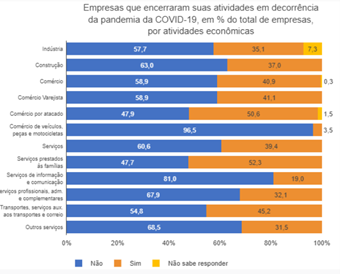
\includegraphics[width=.75\linewidth]{financeira-professor16}
\end{figure}

Trazemos também para a discussão a questão dos direitos trabalhistas e sua efetiva execução. Os aspectos matemáticos, relacionados a capitais equivalentes, ajudam a compreender que o valor do dinheiro no tempo pode estar atrelado a benefícios, mas também a prejuízos, e pensar sobre isso de forma crítica (avaliando diferentes pontos de vistas, pensando de forma ética e fundamentada) é uma marca da nossa proposta, que se alinha com todos os documentos oficiais que balizam a Educação Básica no Brasil, tais como a LDB e a BNCC.
O professor deve observar que essa atividade poderia ser considerada como de juros compostos, sem problema algum. Isso serve para reforçar que problemas de juros compostos são casos particulares de capitais equivalentes, como já apontado no início desta seção.

}{0}{9}
\end{sugestions}

\begin{objectives}{O enigma das taxas de juros invisíveis}
{
\begin{itemize}
\item Investigar situações financeiras que envolvem o valor do dinheiro no tempo, considerando o conceito de capitais equivalentes. 
\item Resolver problemas relacionados aos capitais equivalentes, neste caso a obtenção da taxa de juro de uma proposta de financiamento, na comparação com um valor descontado na compra à vista.
\end{itemize}
}{1}{2}
\end{objectives}
\begin{sugestions}{O enigma das taxas de juros invisíveis}
{
Nessa atividade convidamos o aluno a pensar sobre taxa de juros embutidas em financiamentos diante do desconto no preço de tabela para pagamento à vista. O modelo matemático aqui resulta em uma equação do segundo grau, o que se constitui em uma excelente oportunidade tanto para o professor de matemática do 9º ano do EF, como para o do Ensino Médio quando aborda funções quadráticas ou progressões geométricas. 

Como nosso intuito foi focar na discussão sobre a taxa de juro embutida, essa situação não aborda o tradicional problema de tomada de decisão entre comprar à vista e a prazo, o que demandaria uma taxa mínima de atratividade para o comprador, gerando uma complexidade que intencionalmente não queremos nessa atividade, e precisa de tempo para ser desenvolvida conforme aponta \cite{muniz2016a}.

}{1}{2}
\end{sugestions}
\begin{answer}{Demissão na pandemia}
{
\begin{enumerate}
  \item Os R\$ $100.000$ aplicados em um mês, a uma daxa de $0{,}5$\% resulta em um valor de R\$ $100.500$, pois $1000.000{,}00\times(1+0{,}005)=\text{R\$ }100.500$. Portanto, em maio de 2020, a empresa obteve o valor de R\$ $100.500$ $-$ R\$ $40.000$ $=$ R\$ $60.500$. A partir disto, R\$ $60.500$ aplicados por três meses à mesma taxa de $0{,}5$\% ao mês, resulta em um montante de R\$ $61.412{,}05$, pois $60.400(1+0{,}05)^3=61.412{,}05$. Então, a empresa, em agosto de 2020, ficaria com o valor de R\$ $61.412{,}05-60.000=$R\$ $1.412{,}05$
  \item A empresa não agiu de forma correta, pois não cumpriu o prazo legal das obrigações trabalhistas desrespeitando os diretos dos trabalhadores e ainda se beneficiou com o rendimento de juros que não lhe pertencia quando não devolveu esse dinheiro para os trabalhadores juntamente com a indenização no mês em que o pagamento foi efetuado. É importante também analisar a situação do ponto de vista do empregador, ou seja, ainda que neste caso a empresa tinha dinheiro, em muitos outros isso não necessariamente ocorreu, e a falta de uma estratégia para ajudar a proteger pequenas empresas podem ter ajudado a aumentar as injustiças para os dois lados. 
  \item O impacto na vida dos trabalhadores foi que eles perderam dinheiro com o pagamento da empresa fora do prazo de direito, visto que a empresa não fez o repasse do juro que rendeu cada indenização paga para eles.
\end{enumerate}
}{0}
\end{answer}
\begin{answer}{O enigma das taxas de juros invisíveis}
{
  \begin{enumerate}
    \item Os livros didáticos de matemática apresentariam a solução da seguinte forma. Para encontrarmos a taxa de juros embutida nesta operação, temos que encontrar os valores que satisfazem à seguinte equação: $\displaystyle\frac{4.000}{(1+i)}+\frac{6.000}{(1+i)^2}=9.500$, com $i\geq0$, onde $i$ representa a taxa. Ao resolversmoa a primeira equação, encontramos dois valores, aproximadamente, para a taxa:  $i=0{,}0327$ e $i=-1{,}6116$. Observe que o único valor que satisfaz a ambas equações é $i=0{,}0327$, ou seja, $i=3{,}27$\$

    Uma solução alternativa Uma solução alternativa, que pode ser muito útil \citep{muniz2016b} para convidar os alunos a pensarem a equivalência de capitais na mesma direção da passagem do tempo (do presente para o futuro), seria levar tudo para o futuro, como mostramos a seguir:

    \begin{table}[H]
    \centering
    \renewcommand{\arraystretch}{1.25}
    \begin{tabular}{|c|*{3}{f|}}
    \hline
    \tcolor{} & \tmat{0} & \tmat{1} & \tmat{2} \\
    \hline
    Devo & 9.500 & 9.500f & 9.500f^2-4.000f \\
    \hline
    Pago & 0 & 4.000 & 6.000 \\
    \hline 
    Saldo & 9.500 & 9.500f-4.000 & 0 \\
    \hline
    \end{tabular}
    \end{table}

    \item Para este caso, é necessário resolver a equação $\displaystyle\frac{2.000}{(1+i)}+\frac{8.000}{(1+i)^2}=9.500$, com $i\geq0$, onde $i$ representa a taxa. Ao resolver ja primeira equação, encontramos dois valores, aproximadamente para a taxa: $i=0{,}0289$ e $i=-1{,}8184$. Observe novamente que o único valor que satisfaz a ambas equações para esta seituação é $i=0{,}0289$, ou seja $i=2{,}89$\%. Logo, a taxa da letra \titem{b} é menor que a taxa da letra \titem{a}, pois $2{,}89<3<27$.

    Alternativamente, poderíamos responder à primeira pergunta do item b sem resolver a equação pensando que quanto mais demorar para pagar, menor será a taxa de juro. Olhar para os denominadores é um dos caminhos para se explicar isso. 
  \end{enumerate}
}{0}
\end{answer}

Um erro muito comum é tentar obter o valor acumulado na primeira estratégia, somando as três parcelas de 100 reais, para depois calcular o valor futuro, usando 3 meses como tempo de aplicação por exemplo. Isso não gera o Valor Futuro correto, pois cada parcela teve um tempo de aplicação diferente. Assim, se o dinheiro se transforma no tempo, então só podemos somar quantias se elas estiverem referidas à uma mesma data.

\practice{Capitais Equivalentes}
\label{fin-prac-4}

\begin{task}{Demissão na pandemia}
\label{fin-ativ-19}

Uma empresa demite 10 funcionários em abril de 2020, em função da pandemia, gerando um custo com indenizações totalmente de 100 mil reais. Lamentavelmente, a empresa, mesmo dispondo dos recursos para pagar todas as indenizações, decide pagar dentro do prazo legal (maio de 2020) somente as indenizações de 5 desses funcionários, que totalizaram 40 mil reais, deixando para pagar as outras 5 indenizações, no valor total de 60 mil reais, 3 meses após essa primeira leva, ou seja, em agosta de 2020.
\begin{enumerate}
  \item Se os 100 mil reais foram aplicados a $0{,}5$\% ao mês, qual o valor que a empresa ganhou com essa atitude de atrasar as indenizações dos trabalhadores?
  \item Como você avalia a atitude da empresa?
  \item Apresente possíveis impactos dessa atitude da empresa na vida dos trabalhadores que não tiveram seus direitos trabalhistas respeitados?
\end{enumerate}
\end{task}


\begin{task}{O enigma das taxas de juros invisíveis}
\label{fin-ativ-20}

Calinka comprou um equipamento para sua empresa que reduz a emissão de CO$_2$ na atmosfera, cujo preço de tabela era de 10.000 reais. O vendedor lhe ofereceu $5$\% de desconto na compra à vista. Alternativamente, ela poderia pagar em duas vezes, sendo $40$\% do preço de tabela, um mês após a compra, e $60$\% deste preço dois meses após a compra.
\begin{enumerate}
  \item Qual o valor da taxa de juros embutida nessa operação?
  \item Se os percentuais fossem $20$\% e $80$\%, essa taxa seria maior ou menor? De quanto seria?
\end{enumerate}
\end{task}

\begin{paginatexto}{O valor do dinheiro no tempo: Séries uniformes}

\subsection*{Objetivo geral}
\begin{itemize}
\item Investigar situações financeira que envolvem o valor do dinheiro no tempo, considerando as série uniformes.

\item \textbf{Conceitos abordados}: séries uniformes, anuidades e progressões geométricas, através das habilidades2:
\end{itemize}

\begin{habilities}{EM13MAT101}
 Interpretar situações econômicas, sociais e das Ciências da Natureza
que envolvem a variação de duas grandezas, pela análise dos gráficos das funções representadas e das taxas de variação com ou sem apoio de tecnologias digitais.

\tcbsubtitle{EM13MAT203}
Planejar e executar ações envolvendo a criação e a utilização de aplicativos, jogos (digitais ou não), planilhas para o controle de orçamento familiar, simuladores de cálculos de juros compostos, dentre outros, para aplicar conceitos matemáticos e tomar decisões. 

\tcbsubtitle{EM13MAT507}
Identificar e associar sequências numéricas (PA) a funções afins de domínios discretos para análise de propriedades, incluindo dedução de algumas fórmulas e resolução de problemas.

\tcbsubtitle{EM13MAT508}
Identificar e associar sequências numéricas (PG) a funções exponenciais de domínios discretos para análise de propriedades, incluindo dedução de algumas fórmulas e resolução de problemas.
\end{habilities}

\subsection*{Recomendações para o professor}
\vspace{-1em}
\paragraph{Organização em sala de aula} Essa seção pode ser vista como uma extensão e amplicação das duas anteriores. Vamos investigar situações financeiras em que podemos ter um captial se transformando em uma série uniformes, ou seja, uma série de valores iguais, igualmente distribuídos no tempo. A primeira atividade aponta para isso, e pode ser realizada em grupos de quatro alunos, gerando interação entre os estudantes. Convide seus alunos a criar a cultura de investigar os fundamentos e arazoabilidade das informações veiculadas nas mídias sociais de forma fundamentada.

\paragraph{Dificuldades previstas} Os cálculos agora são bem mais complexos, e podem demandar maior manipulação algébrica envolvendo equações fracionárias. Começar de exmplos com poucos valores, e estruturar o problema usando a representação temporal que priviligeia o presente para o futuro, pode djudar na abordagem do tema.

\paragraph{Sugestões gerais}

Falar sobre capitais equivalentes é falar sobre trocas intertemporais, tendo ou não consciência disso. Reforçamos que nessa seção vamos investigar situações em que podemos ter um ou mais capitais se transformando em ou mais capitais ao longo do tempo.

Primeira sugestão: ir do presente para o futuro é mais intuitivo e costuma ser melhor recebido pelos alunos segundo algumas pesquisas, tais como \cite{campos2013}, \cite{muniz2016b} e \cite{santana2019}, então sugerimos fortemente iniciar com abordagens em que o dinheiro se transforme do presente para o futuro. A seção organizando mostra de forma bem clara um exemplo disso.

Segunda sugestão: comparar os valores em cada data, ainda que se faça isso mais de uma vez, constuma ser melhor, segundo os estudos de \cite{muniz2016a}, do que simplesmente trazer todos os valores do futuro para o presente.

Terceira sugestão: entenda bem, ainda que a equivalência de capitais nos forneça que não nos forneção que não importa a data de comparação de capitais, mas o que importa é que seja a mesma, trabalhar representações temporais do presente para o futuro se alinha com a nossa percepção de tempo, e isso costuma ser muito bem recebido e utilizado pelos alunos.

\paragraph{Enriquecimento da discussão}

É muito comum vermos produtos e serviços sendo oferecidos com opções de pagamento em prestações mensais e iguais. Esse tipo de situação é a forma mais comum de crédito no Brasil. Temos também situações financeiras em que pessoas depositam mensalmente uma mesma quantia para gerar um acumulado no futuro, que para aposentadoria, quer para a compra de um carro, um consórcio ou outro bem, sendo cobradas delas juros ou não na operação.

Mas não são apenas situações de consumos de bens ou serviços. Há investimentos que nos fornecem a opção de recebermos quantias iguais periodicamente, tais como os títulos que pagam juros semestrais, conforme ilustrado na figura a seguir.
\end{paginatexto}

\explore{Séries Uniformes}
\label{fin-exp-5}

É muito comum vermos produtos e serviços sendo oferecidos com opções de pagamento em prestações mensais e iguais. Ou ainda, situações em que pessoas depositam mensalmente uma quantia para gerar um acumulado, quer seja para aposentadoria, quer seja para a compra de um carro, um consórcio, ou outro bem, sendo cobradas delas juros ou não na operação. Você verá que as trocas intertemporais atacam novamente. A figura a seguir é um exemplo desse tipo de situação.

\begin{figure}[H]
\centering

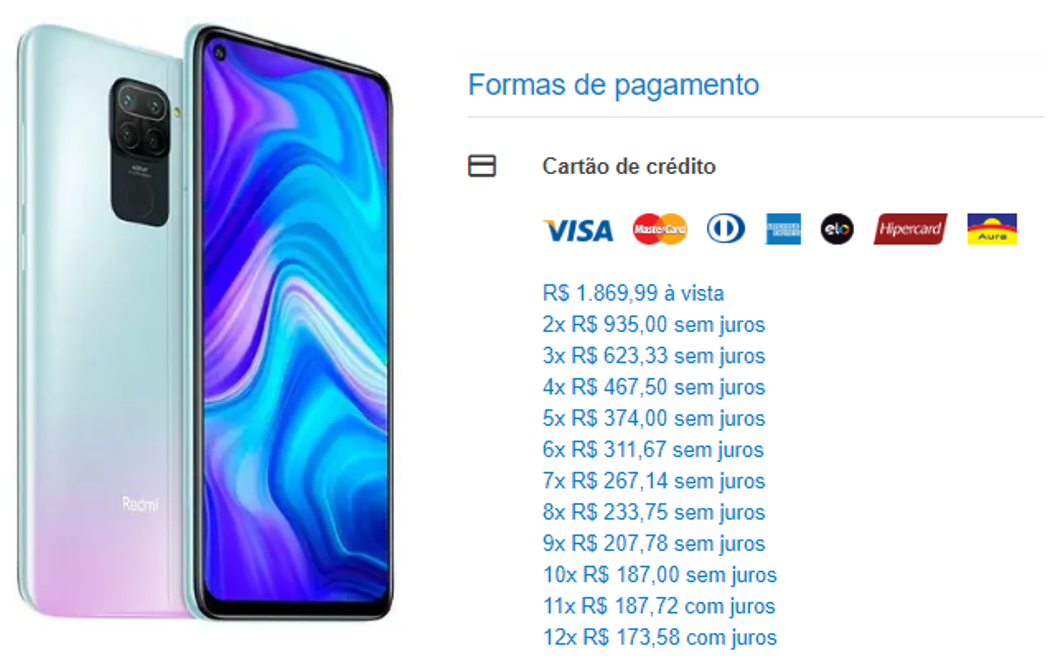
\includegraphics[width=340bp]{financeira12}
\end{figure}

Mas não são apenas situações de consumo de bens ou serviços. Há investimentos que nos fornecem a opção de recebermos quantias iguais periodicamente, tais como os títulos que pagam juros semestrais, conforme ilustrado na figura a seguir.

\begin{figure}[H]
\centering

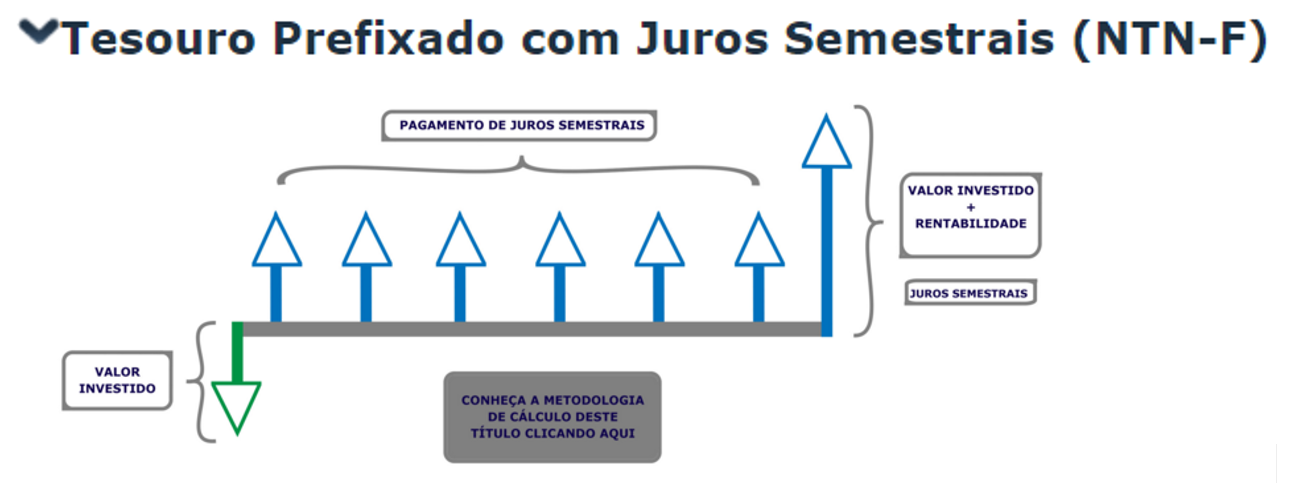
\includegraphics[width=425bp]{financeira13}
\end{figure}

Para começarmos a trabalhar os aspectos matemáticos envolvidos nessas séries de pagamentos iguais e igualmente distribuídos no tempo, chamadas de séries uniformes, bem como aspectos financeiros, econômicos, comportamentais, culturais e sociais presentes nas variadas situações em que as séries uniformes estão presentes, convidamos você a pensar com a gente nessas novas trocas intertemporais.

Vamos começar com a seguinte atividade.
\clearpage
\begin{objectives}{Disciplina e paciência: nascidas uma para a outra!}
{
\begin{itemize}
\item Investigar situações financeiras que envolvem o valor do dinheiro no \item tempo, considerando as Séries Uniformes
\item Resolver problemas relacionados às Séries Uniformes.
\item Analisar como o valor futuro da série é sensível ao tempo de aplicação, por meio de algumas simulações (uma introdução à análise de sensibilidade)
\end{itemize}
}{1}{2}
\end{objectives}
\begin{sugestions}{Disciplina e paciência: nascidas uma para a outra!}
{
Nessa atividade disparadora da seção sobre séries uniformes convidamos o estudante a analisar uma SEF envolvendo uma poupança programada. Deixe os estudantes fazerem estimativas. Se eles não estão familiarizados com o tema, provavelmente apresentarão resultados diferentes do verdadeiro. Ótimo se isso acontecer, pois os modelos aqui são mais elaborados, e as estimativas erradas são excelentes oportunidades de aprendizagem e avaliação do modelo quando ele for construído.
Também queremos convidar o estudante a perceber como o tempo influencia no Valor Futuro da Série Uniforme. 
}{1}{2}
\end{sugestions}
\begin{answer}{Disciplina e paciência: nascidas uma para a outra!}
{
A Atividade será detalhadamente investigada no próximo organizando as ideias.
}{1}
\end{answer}

\begin{task}{disciplina e paciência: nascidas uma para a outra!}
\label{fin-ativ-21}

Considere que Isabel começou a planejar uma boa poupança para realizar alguns sonhos. Para isso resolveu que, a partir de janeiro do próximo ano, aplicará mensalmente 300 reais em um investimento com rentabilidade média de 1\% ao mês. 

\begin{enumerate}
\item Quanto Isabel terá acumulado exatamente após o 4º depósito, ou seja, em abril do próximo ano?
\item E se o tempo de aplicação for de 1 ano? E 20 anos?
\end{enumerate} 

\end{task}

\arrange{Séries Uniformes}
\label{fin-arg-5}

Vamos analisar a situação financeira proposta anteriormente, que envolve uma série de depósitos mensais e iguais, denominada de série uniforme. São as famosas prestações mensais e iguais, muito comuns em financiamentos dos mais variados tipos de produtos e serviços, de eletrodomésticos, carros, a pacote de férias e seguros. Essa é a última situação que analisaremos antes de passarmos uma investigação da atividade inicialmente apresentada na seção.

Vamos começar investigando quanto Isabel terá acumulado imediatamente após o $^{\circ}$ depósito, ou seja, em abril do próximo ano.

A representação temporal abaixo ilustra o fluxo de depósitos que será realizado no período de janeiro a abril, bem como o valor futuro de cada quantia depositada nesses quatro meses.

\begin{table}[H]
\centering
\begin{tabular} {|c|c|c|c|}
\hline
\tmcol{4}{|c|}{Isabel}\\
\hline
Janeiro & Fevereiro & março & abril \\
\hline
\def\currentcolor{session4!50}
\tcolor{300} \tikzmark{a} & & &\tikzmark{b} 309,09 \\
\hline
& \tcolor{300} \tikzmark{c} & & \tikzmark{d}
 306,03 \\
\hline 
& & \tcolor{300} \tikzmark{e} & \tikzmark{f}
 303{,}00 \\
 \hline
& & & \tcolor{300{,}00}\\
\hline

\end{tabular}
\end{table}
% \begin{tikzpicture}[overlay, remember picture, shorten >=.5pt, shorten <=.5pt,transform canvas={yshift=.13cm}]

% \draw [->, very thick, \currentcolor] ({pic cs:a}) to ({pic cs:b});
% \draw [->, very thick, \currentcolor] ({pic cs:c}) to ({pic cs:d});
% \draw [->, very thick, \currentcolor] ({pic cs:e}) to ({pic cs:f});

% \end{tikzpicture}

Assim, o valor futuro total imediatamente após os 4 depósitos pode ser calculado somando-se o valor futuro de cada depósito em abril daquele ano,

$$\mathit{VF}_4=300\times1{,}01^3+300\times1{,}01^2+300\times1{,}01^1+300=1.218{,}12$$

Em vez de calcular essas quatro parcelas e somá-las, também poderíamos pensar assim:

\begin{equation*}
\mathit{VF}_4=300\times1{,}01^3+300\times1{,}01^2+300\times1{,}01^1+300
\end{equation*}

Multiplicando ambos os lados da equação por $1{,}01$, temos:

\begin{equation*}
1{,}01\times \mathit{VF}_4=300\times1{,}01^4+300\times1{,}01^3+300\times 1,01^2+300\times1{,}10
\end{equation*}

Subtraindo as duas equações, chegamos ao seguinte resultado:

\begin{align*}
1{,}01\times \mathit{VF}_4-\mathit{VF}_4&=300\times1{,}01^4-300\\
\mathit{VF}_4(1{,}01-1)&=300(1{,}01^4-1)\\
\mathit{VF}_4&=\frac{300(1{,}01^4-1)}{1{,}01-1}=1.218{,}12
\end{align*}

Ainda poderíamos ter um terceiro caminho, que é perceber que essa sequência de pagamentos é uma progressão geométrica, com o primeiro termo igual a $300$ e razão igual $1{,}01$.

\textbf{Você percebeu que temos uma soma de uma P.G.?}

Nesse caso, o $\mathit{VF}$ é igual à soma dos primeiros quatro termos dessa progressão gemétrica. Assim, também podemos calcular o valor futuro usando o seguinte resultado.

Dada uma progressão geométrica, de termo inicial $a_1$ e razão $q$, a soma dos $n$ primeiros termos dessa progressão é dada por:

\begin{equation*}
S_n=\frac{a_1(q^n-1)}{q-1}
\end{equation*}
 
Assim, usando essa expressão que fornece a soma dos termos de uma progressão geométrica, o valor $\mathit{VF}$ pode ser obtido por:

\begin{align*}
\mathit{VF}_4&=\frac{300(1{,}01^4-1)}{1{,}01-1}\\
\mathit{VF}_4&=1.218{,}12
\end{align*}

Um dos benefícios de se usar a soma dos termos de uma P.G., é poder usar um mesmo modelo matemático independente do prazo, ou seja, para qualquer quantidade de depósitos ou pagamentos. De fato, usando a mesma lógica nessa operação, o $\mathit{VF}$ para um prazo igual a 12 meses, ou seja, o $\mathit{VF}$ imediatamente após o 12º depósito, é igual a

\begin{align*}
\mathit{VF}_{12}&=\frac{300(1{,}01^{12}-1)}{1{,}01-1}\\
\mathit{VF}_{12}&=3.804{,}75
\end{align*}

E para um prazo ainda maior, de 240 meses (20 anos) de depósitos (haja disciplina e paciência!), usando a mesma lógica da operação anterior, temos que o $\mathit{VF}$ imediatamente após o 240º depósito, é igual a:

\begin{align*}
\mathit{VF}_{240}&=\frac{300(1{,}01^{240}-1)}{1,01-1}\\
\mathit{VF}_{240}&=296.776{,}61
\end{align*}

Esse valor nos mostra que as 240 aplicações de 300 reais, realizadas todos os meses, geraram quase 300 mil reais ao final do período, a uma taxa de $1$\% ao mês. 


Mas será que essa taxa de $1\%$ ao mês? realmente existe e está acessível a todos? Isso vai depender de diversos fatores, dentre eles o momento econômico. Em março de 2016, por exemplo, essa taxa era acessível a qualquer cidadão que fizesse um investimento chamado tesouro pré-fixado, que pagava à época 14,47\% ao ano, conforme ilustra a figura a seguir.

\begin{figure}[H]

\centering
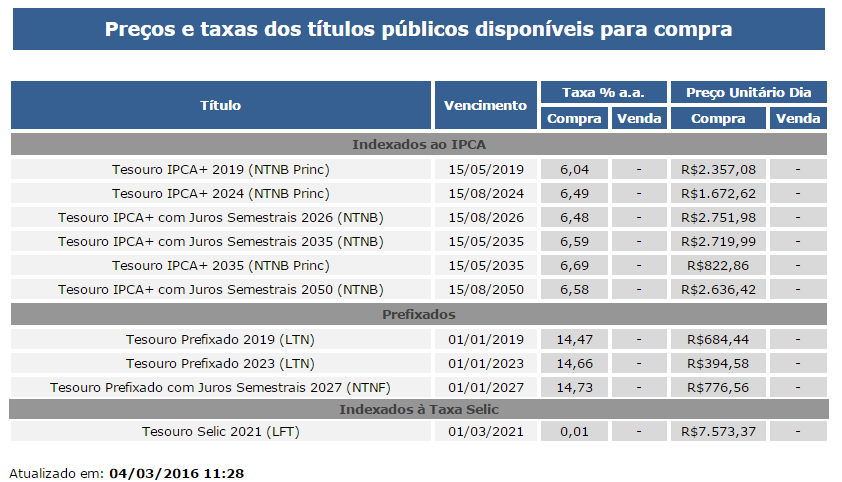
\includegraphics[width=375bp]{taxas-titulos-publicos}
\caption{Fonte: \href{http://www.tesouro.fazenda.gov.br/tesouro-direto-precos-e-taxas-dos-titulos}{Tesouro Nacional}, acessado em 04/03/2016}

\end{figure}

Mas em setembro de 2019, 3,5 anos depois, a taxa de 1\% ao mês já não estava mais disponível, e o mesmo tipo de título prefixado pagava 5,97\% ao ano, conforme se pode observar na figura a seguir.

\begin{figure}[H]

\centering
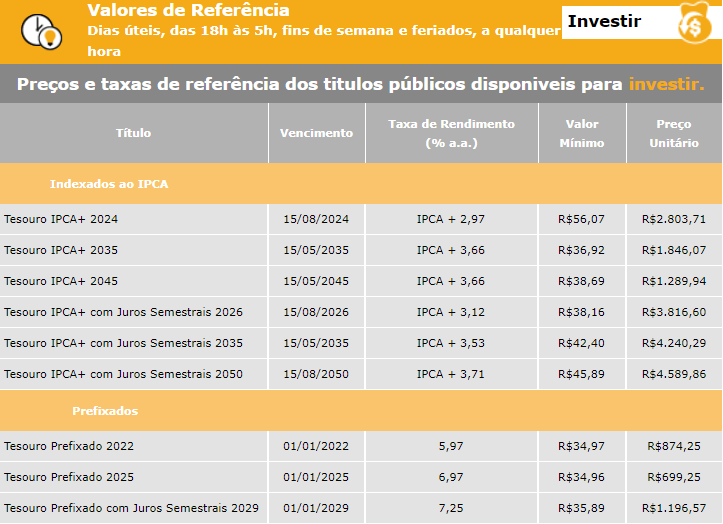
\includegraphics[width=375bp]{taxas-titulos-publicos-2}
\caption{Fonte: \href{http://www.tesouro.fazenda.gov.br/tesouro-direto-precos-e-taxas-dos-titulos}{Tesouro Nacional}, acessado em 04/09/2019}

\end{figure}

Essas diferentes taxas podem gerar grandes diferenças no $\mathit{VF}$ de uma série uniforme. Podemos investigar como a taxa influencia/impacta o $\mathit{VF}$ total acumulado, realizando o que chamamos de análise de sensibilidade, que é uma simulação do $\mathit{VF}$ para diferentes taxas. A tabela e o gráfico a seguir ilustram uma análise de sensibilidade para o caso de 240 depósitos mensais de 300 reais.

\begin{table}[H]
\centering
\begin{tabular} {|c|c|}
\hline
\tcolor{Taxa Mensal} & \tcolor{Valor Futuro} \\
\hline
0,40\% & R\$ 120.502,51 \\
\hline
0,50\% & R\$ 138.612,27 \\
\hline
0,60\% & R\$ 160.128,70 \\
\hline
0,70\% & R\$ 185.752,34 \\
\hline
0,80\% & R\$ 216.339,37 \\
\hline
0,90\% & R\$ 252.925,33 \\
\hline
1{,}00\% & R\$ 296.776,61 \\
\hline
1,50\% & R\$ 692.656,31 \\
\hline
2{,}00\% & R\$ 1.723.331,03 \\
\hline
2,50\% & R\$ 4.484.855,58 \\
\hline
3{,}00\% & R\$ 12.038.526,28 \\
\hline
5{,}00\% & R\$ 730.431.442,45 \\
\hline
\end{tabular}
\caption{Fonte: Elaborado pelo autor}
\end{table}

\begin{figure}[H]
\centering\resizebox{.85\linewidth}{!}
{

\begin{tikzpicture}[yscale=0.5, scale=0.7]

\foreach \x in{2,4,6,8}  \draw [gray!70, thin] (0,\x) -- (19.5,\x) node [black, pos=0.0,left, scale=0.8] {\x00.000{,}00}; 
\foreach \x/\y in{10/1.0,12/1.2,14/1.4,16/1.6,18/1.8,20/2.0}  \draw [gray!70, thin] (0,\x) -- (19.5,\x) node [black, pos=0.0,left, scale=0.8] {\y00.000{,}00}; 
\draw (0,0) -- (19.5,0) node [black, pos=0.0,left,scale=0.8] {0{,}00};

\coordinate (a) at (1,1.2050251);
\coordinate (b) at (2.2,1.3861227);
\coordinate (c) at (3.4,1.6012870);
\coordinate (d) at (4.6,1.8575234);
\coordinate (e) at (5.8,2.1633937);
\coordinate (f) at (7,2.5292533);
\coordinate (g) at (8.2,2.9677661);
\coordinate (h) at (9.4,4.1278149);
\coordinate (i) at (11.8,5.8127313);
\coordinate (j) at (14.2,8.2748538);
\coordinate (k) at (16.6,11.8924492);
\coordinate (l) at (19,17.2333103);

\draw [very thick,\currentcolor](a)--(b)--(c)--(d)--(e)--(f)--(g)--(h)--(i)--(j)--(k)--(l);
\foreach \x in {a,b,...,l} \node [circle, fill=\currentcolor, minimum size=4pt, inner sep=0pt] at (\x) {};

\node at (9,21.5) {Sensibilidade do Valor Futuro a taxa mensal de Retorno};
\foreach \x/\y in {1/{0,40\%},2.2/{0,50\%},3.4/{0,60\%},4.6/{0,70\%},5.8/{0,80\%},7/{0,90\%},8.2/{1{,}00\%},9.4/{1,20\%},11.8/{1,40\%},14.2/{1,60\%},16.6/{1,80\%},19/{2{,}00\%}} \node [below, scale=0.65] at (\x,0) {\y};


\end{tikzpicture}.
}
\end{figure}

As simulações nos permitem fazer uma análise de sensibilidade do valor acumulado ($\mathit{VF}$) em relação à taxa de retorno do investimento, para um mesmo prazo. Elas nos mostram que para uma taxa de 0,5\%, o $\mathit{VF}$ é de 138 mil reais, menos que a metade dos 297 mil reais obtidos na atividade que trazia uma taxa de 1,0\% ao mês. 

Mas como obter taxas maiores? Uma das formas de se tentar obter maiores taxas de retorno é considerar investimentos mais arriscados. Mas isso é conversa para a próxima seção

\begin{knowledge}

A taxa de 0,5\% ao mês foi aproximadamente a remuneração da poupança – modalidade de “investimento” mais popular entre os brasileiros, em setembro de 2019

\end{knowledge}

\clearpage
\clearmargin
\clearmargin
\begin{objectives}{O dilema de caber no bolso - parcelas mensais e iguais}
{
\begin{itemize}
\item item Investigar situações financeiras que envolvem o valor do dinheiro no tempo, considerando as Séries Uniformes
\item Resolver problemas relacionados às Séries Uniformes.
\item Analisar como a taxa de retorno da pessoa, caso possua dinheiro investido, pode influenciar na tomada de decisão em parcelamentos mais longos.
\end{itemize}
}{1}{2}
\end{objectives}
\begin{sugestions}{O dilema de caber no bolso - parcelas mensais e iguais}
{
Essa atividade tem alguns (poucos) elementos das atividades tradicionais de séries uniformes encontradas em livros didáticos de matemática, e vários elementos diferentes. 

A questão começa com duas perguntas abertas e, portanto, livres. Elas convidam o aluno a falar sobre suas escolhas e justificá-las, como se ele fosse o personagem da história. Se colocar no lugar do outro é um exercício importante pois além de mostrar um pouco como os alunos pensam a situação, como operam, julgam, avaliam e decidem, podem evidenciar aspectos não matemáticos, tais como os culturais, econômicos e sociais.

Será que o critério de caber no bolso será usado pelos alunos? Ou eles vão preferir fugir dos juros, mesmo que para isso escolham uma prestação um pouco maior que o planejado? Utilizarão algum cálculo ou processo, ou vão mobilizar o sistema 1 – aquele rápido e preguiçoso – para tomar a decisão.

Depois disso, o item c foca no processo de determinar a prestação de uma série uniforme postecipada, ou seja, aquela cujo valor atual da série está um período antes da série começar. De uma maneira prática, compra hoje, mas começa a pagar daqui a 1 mês. Esse item é tradicional, e daí o professor pode usar vários caminhos, desde a aplicação de uma fórmula, ao uso de simuladores em aplicativos ou até mesmo planilhas eletrônicas. Aqui busque o princípio da dualidade: educação financeira para aprender matemática e produzir matemática para aprender sobre situações financeiras. Dois lados de uma mesma ... educação financeira. 

Finalmente o item d temos um outro tipo de tomada de decisão, na qual a pessoa tem dinheiro investido a $0{,}6\%$ ao mês. Com isso, o valor do dinheiro no tempo pode influenciar a vantagem financeira de opções de pagamento com prazos mais dilatados. Cuidado. Será necessário usar a taxa da pessoa para transformar os valores das parcelas. 

}{1}{2}
\end{sugestions}

\begin{answer}{O dilema de caber no bolso - parcelas mensais e iguais}
{
\begin{enumerate}
\item Resposta pessoal.
\item Resposta pessoal.
\item O valor "à vista é R\$ $829{,}45$". A taxa de juros é de $1{,}29\%$ ao mês. O prazo é de 12 meses. Para calcular o valor da prestação podemos usar:
\begin{equation*}
A=\frac{P}{(1+i)^n}\times\frac{(1+i)^n-1}{i}.
\end{equation*}
Esse é o valor atual de uma série de $n$ parcelas iguais a $P$, um período antes dela começar, a uma taxa $i$ ao período.

Isolando $P$, temos
\begin{align*}
P&=A\times\frac{(1+i)^n\cdot i}{(1+i)^n-1} \\
P&=829{,}45\times\frac{(1+0{,}0129)^{12}\cdot0{,}0129}{(1+0{,}0129)^{12}-1}\\
P&=829{,}45\times0{,}09048497\\
P&=75{,}05
\end{align*}

\item Impressionante e inexplicavelmente, no parcelamento apresentado, o valor do frete é considerado na história, e com isso $A=849{,}00+22{,}90=871{,}90$. Perceba que o valor à vista tem um desconto. Mas isso não fica muito claro na tela final de compra. Recalculando, temos o seguinte:
\begin{align*}
P&=A\times\frac{(1+i)^n\cdot i}{(1+i)^n-1} \\
P&=871{,}90\times\frac{(1+0{,}0129)^{12}\cdot0{,}0129}{(1+0{,}0129)^{12}-1}\\
P&=871{,}90\times0{,}09048497\\
P&=78{,}89
\end{align*}

\end{enumerate}
}{1}
\end{answer}
\begin{answer}{O dilema de caber no bolso - parcelas mensais e iguais}
{
\begin{enumerate}\setcounter{enumi}{4}
\item Para tomar a decisão considerando a taxa de retorno de $0{,}6\%$ ao Mês do comprador, podemos dentre várias estratégias, calcular o valor atual dos fluxos por essa taxa. Assim, temos:
\begin{align*}
A&=\frac{99{,}32}{1{,}006^9}\times\frac{(1{,}006^9-1)}{0{,}006}\\
A&=869{,}64\\
A&=\frac{89{,}61}{1{,}006^10}\times\frac{(1{,}006^10-1)}{0{,}006}\\
A&=867{,}22
\end{align*}

Veja que é mais vantajoso, ainda que a diferença seja nesse caso muito pequena, pagar em 10X. Uma outra forma de olhar: posso pagar um valor mais baixo com um prazo um pouco maior, gastando praticamente a mesma coisa se eu levar em conta o valor do dinheiro no tempo. Ou seja, ele pode optar por pagar mais folgado levando em conta o dinheiro que tem, se pagar em 10x.

Além disso, observe que se um aluno somasse o valor das prestações ele acharia que a mais vantajoso do ponto de vista financeiro é pagar em 9x. 

\begin{align*}
9\times99{,}32&=99{,}32-893{,}88\\
10\times89{,}61&=896{,}10
\end{align*}

Mas dessa forma tomaria uma decisão diferente daquela levando em consideração o dinheiro no tempo. 
\end{enumerate}
}{9}
\end{answer}

\begin{example}{Retomando a atividade inicial}
\label{fin-exemp-1}

Você tem duas possibilidades de fazer uma poupança:
\begin{itemize}
\item Investir 200 reais por mês durante 20 anos
\item Investir 400 reais por mês durante 10 anos, parar de depositar, deixando o acumulado rendento até completar 20 anos.

\end{itemize}

Considere que o dinheiro renda 1\% ano mês, rendendo sempre sobre o saldo acumulado da sua poupança.

\begin{enumerate}

\item Qual a melhor estratégia que gera o maior valor acumulado ao final de 20 anos?

\item Qual a melhor estratégia do seu ponto de vista? Justifique sua resposta

\item O que isso tem a ver com a discussão atual (2019) sobre a reforma da previdência?

\end{enumerate}

Para responder à primeira pergunta, basta observar que como o valor nominal investido é o mesmo, e a taxa também é a mesma em ambas, então, quanto antes investirmos, melhor. Logo a segunda gera um valor futuro maior.

Também poderíamos usar matemática para encontrar a estratégia que gera o maior valor acumulado. Para isso, basta calcular o valor futuro de cada uma das séries uniformes produzidas em cada estratégia. 

Para a primeira estratégia, vamos admitir, sem perda de generalidade, que na primeira situação, o primeiro depósito de 200 reais seja realizado em jan/2020 e o último em dez/2039. Assim, o $\mathit{VF}$ dessa série uniforme em dez/2039 será: 


\begin{align*}
\mathit{VF}_{\text{estratégia I}}&=\frac{200(1{,}01^{240}-1)}{1{,}01-1}\\
\mathit{VF}_{\text{estratégia I}}&=197.851{,}08
\end{align*}

Na segunda estratégia, temos duas fases de investimento, em que o valor futuro da série uniforme com prazo de 120 meses, obtido em dez/2029, é atualizado por mais 120 meses, até dez/2039. Logo, 

\begin{align*}
\mathit{VF}_{\text{estratégia II}}&=\frac{400(1,01^{120}-1)\times1{,}01^{120}}{1,01-1}\\
\mathit{VF}_{\text{estratégia II}}&=303.686,67
\end{align*}

Os cálculos nos levam ao que já sabíamos, sem fazer as contas: a segunda estratégia é mais vantajosa do ponto de vista do valor acumulado ao final do período.

A segunda pergunta, é aberta. Ela pode parecer sem sentido, mas não é. Para quem tem dificuldades orçamentárias (ou tem rendas menores) a primeira estratégia pode ser a melhor por ser a mais viável, ou a menos sacrificante. Do ponto de vista comportamental, pode ser mais fácil manter a disciplina de guardar 200 reais mensais do que 400. Isso vai depender de uma série de fatores orçamentários, comportamentais e aleatórios – a probabilidade de conseguir gerir uma saída de caixa de 200 reais, diante de imprevistos e demandas não planejadas é a mesma com uma saída de 400 reais?

A terceira pergunta nos convida a refletirmos sobre as variáveis tempo de contribuição e valor de contribuição. 
\end{example}

Se não podemos, em muitos casos, obter taxas maiores sem pôr em risco o dinheiro poupado muitas vezes como muitas dificuldades e sacrifícios, então será que podemos ampliar o tempo de contribuição, começando a investir antes por exemplo? 

É possível num país como o Brasil, começar a poupar mais cedo? O valor futuro acumulado será suficiente para gerar os pagamentos mínimos necessários, no período de recebimentos? Essas são questões importantes, e com as quais a poupulação tem se preocupado 2020 com as novas regras previdenciárias.

Para finalizar, vamos generalizar alguns resultados sobre séries uniformes, a partir das experiências com as investigações anteriores.

\textbf{Quando vale uma série de $\bm{n}$ recebimentos mensais e iguais a $\bm{P}$, a uma taxa $\bm{i}$, um período antes dela começar?}

Vamos chamar esse valor presente da série, um período antes dela começar, de valor atual ($A$) da série.

Para responder a essa pergunta, podemos pensar em cada parcela separadamente e descobrir quanto precisamos depositar hoje para receber $P$ daqui a um mês, dois meses, três meses e assim por diante até $n$ meses. Ou seja, podemos calcular o valor presente de cada uma das parcelas de valor $P$. O esquema abaixo ilustra esse movimento do dinheiro no tempo.

\begin{table}[H]
\centering
\begin{tabular} {|c|c|c|c|c|c|}
\hline
\tcolor{Hoje} & \tcolor{Parcela 1} & \tcolor{Parcela 2} & \tcolor{Parcela 3} & \tcolor{\phantom{Parcela 3}} & \tcolor{Parcela $\bm{n}$} \\
\hline
$\displaystyle\frac{P}{(1+i)}$\tikzmark{b} & \tikzmark{a}$P$ & & & & \\
\hline
$\displaystyle\frac{P}{(1+i)^2}$\tikzmark{d} & & \tikzmark{c}$P$ & & & \\
\hline
$\displaystyle\frac{P}{(1+i)^3}$\tikzmark{f} & & & \tikzmark{e}$P$ & & \\
\hline
$\vdots$ & $\vdots$ & $\vdots$ & $\vdots$ & $\vdots$ & $\vdots$ \\
\hline
$\displaystyle\frac{P}{(1+i)^n}$\tikzmark{h} & & & & & \tikzmark{g}$P$ \\
\hline
\end{tabular}

\begin{tikzpicture}[overlay, remember picture, shorten >=1pt, shorten <=.5pt,transform canvas={yshift=.13cm}]

\draw [->, very thick, \currentcolor] ({pic cs:a}) to ({pic cs:b});
\draw [->, very thick, \currentcolor] ({pic cs:c}) to ({pic cs:d});
\draw [->, very thick, \currentcolor] ({pic cs:e}) to ({pic cs:f});
\draw [->, very thick, \currentcolor] ({pic cs:g}) to ({pic cs:h});

\end{tikzpicture}
\end{table}

Assim, o valor atual $A$ de uma série de $n$ parcelas, um período antes dela começar, é igual à soma dos valores presentes de cada uma das parcelas.

De outra forma, o valor que eu preciso investir hoje, para ter $n$ recebimentos iguais a $P$ em suas respectivas datas, ao longo do tempo, é igual ao somatório do valor presente de cada uma das parcelas hoje.

Assim, poremos concluir que

\begin{align*}
A&=\frac{P}{(1+i)}+\frac{P}{(1+i)^2}+\frac{P}{(1+i)^3}+\cdots+\frac{P}{(1+i)^n}\\
A&=\frac{P}{(1+i)^n}\times\frac{(1+i)^n-1}{(1+i)-1}\\
A&=\frac{P}{(1+i)^n}\times\frac{(1+i)^n-1}{i}
\end{align*}

\textbf{Esse é o valor atual de uma série de $n$ parecelas iguais a $P$, um período antes dela começar}.

Com essa expressão, podemos analisar diversas situações envolvendo as séries uniformes, incluindo as situações envolvendo as tão famosas compras em parcelas mensais e iguais com juros. Determinar o valor da prestação, a taxa de juros embutida em um financiamento, e o prazo necessário para se atingir metas nessas situações, também podem ser feitas por meio dessa expressão.



\begin{task}{O dilema de caber no bolso - parcelas mensais e iguais}
\label{fin-ativ-22}

O Sr. Muniz resolveu comprar uma bike de presente para seu filho Arthur. Mas não vai conseguir pagar à vista dessa vez, como costuma fazer. Ele se planejou para pagar no máximo 100 reais de prestação, em um prazo máximo de um ano. A figura abaixo representa o valor da bike e as condições de parcelamento na compra a prazo.


\begin{figure}[H]
\centering

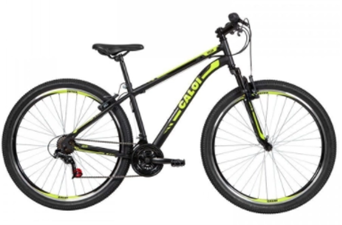
\includegraphics[width=.6\linewidth]{financeira55}
\end{figure}

\begin{figure}[H]
\centering

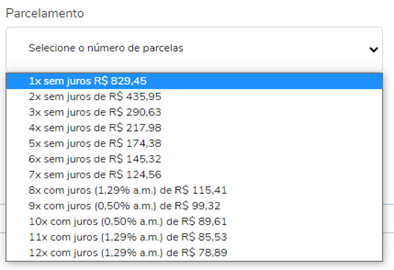
\includegraphics[width=.6\linewidth]{financeira56}
\end{figure}

\begin{enumerate}
\item Qual opção de parcelamento você escolheria se estivesse no lugar do Sr. Muniz?
\item Se você estivesse no lugar do Arthur e pudesse ajudar seu pai a escolher, qual seria a sua sugestão?
\item Calcule o valor da prestação, considerando a compra em 12x com juntos de $1{,}29\%$ a.m. e o valor de R\$ $829{,}45$ com sendo o valor à vista. 
\item Porque o valor apresentado de R\$ $78{,}89$ é maior que o calculado por você? Explique matematicamente, considerando as informações adicionais apresentadas que \textbf{só aparecem para o cliente} no final da tela de compra no site.

\begin{figure}[H]
\centering

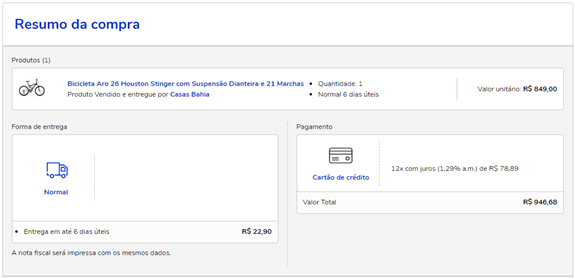
\includegraphics[width=.75\linewidth]{financeira57}
\end{figure}

\item Se o Sr. Muniz tivesse 1000 reais aplicados a $0{,}6\%$ ao mês, qual das duas opções seria mais vantajosa (do ponto de vista exclusivamente financeiro)?

\begin{enumerate}[label=\Roman* -]
\item Comprar em 9x de R\$ $99{,}32$
\item Comprar em 10x de R\$ $89{,}61$
\end{enumerate}
\end{enumerate}
\end{task}

\begin{reflection}
Podemos ainda, a partir do Valor Atual da série, obter o Valor Futuro ($\mathit{VF}$) da mesma série, ou seja, o Valor da série na data da última parcela (incluindo-a), transformando esse valor no tempo. Para isso, basta multiplicar o valor atual por $(1+i)^n$.

Nesse caso, teríamos:


\begin{align*}
\mathit{VF}&=A\times(1+i)^n\\
\mathit{VF}&=\frac{P}{(1+i)^n}\times\frac{(1+i)^n-1}{i}\times(1+i)^n\\
\mathit{VF}& =P\times\frac{(1+i)^n-1}{i}
\end{align*}



Veja que essa expressão é a generalização do que tínhamos obtido como solução para a última atividade, a partir da soma de uma progressão geométrica.

\begin{align*}
\mathit{VF}_{\text{estratégia I}}&=\frac{200(1{,}01^{240}-1)}{0{,}01}\\
\mathit{VF}_{\text{estratégia I}}&=197.851{,}07
\end{align*}

Vemos aqui que podemos usar objetos matemáticos, operações e lógicas diferentes para produzir significados e investigar a situação financeira posta por diferentes caminhos.

Na última atividade, vamos refletir sobre objetos matemáticos, operações e lógicas diferentes para produzir significados e investigar a situação financeira posta por diferentes caminhos.
\end{reflection}
\clearpage


\def\currentcolor{session2}
\begin{objectives}{O que será o amanhã?}
{
\begin{itemize}
\item Investigar situações financeiras que envolvem o valor do dinheiro no tempo, considerando as Séries Uniformes
\item Resolver problemas relacionados às Séries Uniformes.
\item Analisar como o valor futuro da série é sensível ao tempo de aplicação, por meio de algumas simulações (uma introdução à análise de sensibilidade)
\end{itemize}
}{1}{1}
\end{objectives}
\begin{sugestions}{O que será o amanhã?}
{
Nessa atividade convidamos o aluno a usar os modelos construídos sobre valor presente e valor futuro de uma série para investigar uma situação financeira muito comum a milhões de brasileiros: contribuições mensais visando a aposentadoria. Temas atuais (olhando para 2019/2020) como a Reforma da Previdência (já sancionada) e Reforma Trabalhista (atualmente em discussão) são ótimas oportunidades para se pensar a realidade das famílias dos alunos, e o futuro dos próprios alunos. 

Os modelos aqui estão associados às progressões geométricas, em especial a soma de termos de uma P.G. Sugerimos bastante treino para que os alunos possam pensar com desenvoltura tais problemas e situações. Na seção de exercícios apresentamos várias SEF na forma de problemas inclusive que podem ser utilizados. Mas o professor pode criar os seus próprios problemas. 

O professor pode usar simuladores prontos e as planilhas eletrônicas para facilitar as simulações e análises de sensibilidade, ou seja, quando o foco for investigar o comportamento de uma variável em função de outra, mantendo todas as outras constantes. 

Por fim, procuramos trazer para essa atividade uma discussão sobre o impacto da inflação no poder de compra do valor futuro da série. O professor pode optar por discutir em outro momento, por exemplo, depois da abordagem da relação entre inflação e poder de compra (Efeito Fischer) que faremos em uma seção específica mais à frente.
}{1}{1}
\end{sugestions}
\begin{answer}{O que será o amanhã?}
{
  \begin{enumerate}
    \item A resposta é pessoal. Algumas possibilidades, dentre muitas, são: disciplina para manter isso durante tanto tempo, a manutenção dessa taxa de juros, resistir aos desejos de gastar o dinheiro acumulado em algum momento, não precisar gastar as reservas devido a emergências.
    \item Ele fará 12 depósitos mensais durante 40 anos, logo fará 480 depósitos.
    \item O valor da quantia pode ser calculado assim:
    \begin{align*}
      A&=\frac{20.000(1{,}005^180-1)}{1{,}005^{180}\times(1{,}005^{180}-1)}\\
      A&=2.370.070{,}29.
    \end{align*}
    Esse é o valor que a pessoa precisa ter abumulado, em dez/2060, para receber uma série de pagamentos de 15 mil reais, com o primeiro em jan/2061 e o último em dez/2075.

    Agora, basta calcular qual o valor da quantia que precisa ser depositada mensalmente durante os quarenta anos para produzir esse acumulado, considerando as datas estabelecidas, o que pode ser feito assim:
    \begin{align*}
      P_1&=\frac{2.780.070{,}29)\times(1{,}005-1)}{(1{,}005^{180}-)}\\
      P_1&=\text{R\$ }1.190{,}10.
    \end{align*}

    Nos quadros a seguir, temos um resumo da operação usando as funções financeiras de uma planilha eletrônica.

    \begin{multicols}{2}

      \begin{table}[H]
      \centering

      \begin{tabular}{|c|r|}
      \hline
      \tmcol{2}{|c|}{1\textsuperscript{a} Operação} \\
      \hline
      PMT & 20.000 \\
      \hline
      $n$ & 180 \\
      \hline
      $i$ & $0{,}50$\% \\
      \hline
      $\mathit{VP}$ & R\$ $2.380.070{,}29$ \\
      \hline
      \end{tabular}
      \end{table}

      \begin{table}[H]
      \centering

      \begin{tabular}{|c|r|}
      \hline
      \tmcol{2}{|c|}{2\textsuperscript{a} Operação} \\
      \hline
      $\mathit{VF}$ & R\$ $2.370.070{,}29$ \\
      \hline
      $n$ & 480 \\
      \hline
      $i$ & $0{,}50$\% \\
      \hline
      PMT & R\$ $1.190{,}10$ \\
      \hline
      \end{tabular}
      \end{table}
    \end{multicols}

    \begin{table}[H]
    \centering

    \begin{tabular}{|c|c|c|c|}
    \hline
    \tmcol{2}{|c|}{Tempo de contribuição} & \tmcol{2}{c|}{Tempo de recebimentos} \\
    \hline
    fez 25 anos & & fez 65 anos & \\
    \hline
    jan/21 & dez/60 & jan/61 & dez/75 \\
    \hline
    depósito 1 & depósito 300 & renda 1 & renda 180 \\
    \hline 
    R\$ $1.180{,}10$ & R\$ $1.180{,}10$ & R\$ $20.000{,}00$ & R\$ $20.000{,}00$ \\
    \hline
    \end{tabular}
    \end{table}

    \item Considerando a inflação de $3$\% ao ano, uma pessoa vai conseguir comprar com 20.000 reais o que consegue comprar hoje com
    \begin{align*}
      \mathit{VP}&=\frac{2.000}{1{,}03^{40}}\\
      \mathit{VP}&=\text{R\$ }5.131{,}14.
    \end{align*}
    Isso significa que uma pessoa precisará ganhar 20 mil reais daqui a 40 anos para manter o padrão de compra de uma pessoa que ganha, nos dias atuais, aproximadamente 6 mil reais. É preciso levar em consideração a inflação nessa estratégia, para não correr o risco de achar que um determinado valor vai poder suprir as necessidades de uma fase da vida com mais desafios e menor força de trabalho.
  \end{enumerate}
}{9}
\end{answer}

\practice{Séries Uniformes e Previdência}
\label{fin-prac-5}

\begin{task}{O que será o amanhã?}
\label{fin-ativ-23}

Suponha que uma pessoa vai completar 25 anos em janeiro 2021 e planeje a partir dessa data investir mensalmente uma quantia fixa, de modo a assegurar uma aposentadoria complementar de 20 mil reais durante 15 anos, sendo o primeiro depósito em jan/2021 e o último em dez/2060. Considerando uma taxa média de retorno desses investimentos de $0{,}5$\% a.m., uma expectativa de vida de 80 anos, e que o primeiro benefício seja recebido em jan/2061 e o último em dez/2075, determine:
\begin{enumerate}
  \item quais são os dois principais desafios para a concretização dessa estratégia, na sua opinião;
  \item quantos depósitos mensais ele fará até se aposentar e quantos benefícios ele receberá;
  \item o valor da quantia mensal a ser investida;
  \item qual será o valor de compra o valor de compra dos 20 mil reais que ele vai começar a receber em jan/2061, considerando uma inflação anual de $3$\% ao ano?
\end{enumerate}
\end{task}

\begin{paginatexto}{Velozes e furiosas: taxas de juros no cenário brasileiro}

\raggedcolumns
\subsection*{Objetivos gerais}

\begin{itemize}
\item Investigar situações financeiras que envolvem o valor do dinheiro no tempo, considerando taxas equivalentes.

\item \textbf{Conceitos abordados}: taxas de juros, equivalência de taxas e progressões geométricas, através das habilidades
\end{itemize}

\begin{habilities}{EM13MAT101}
 Interpretar situações econômicas, sociais e das Ciências da Natureza
que envolvem a variação de duas grandezas, pela análise dos gráficos das funções representadas e das taxas de variação com ou sem apoio de tecnologias digitais.

\tcbsubtitle{EM13MAT104}

Interpretar taxas e índices de natureza socioeconômica, tais como índice de desenvolvimento humano, taxas de inflação, entre outros, investigando os processos de cálculo desses números.

\tcbsubtitle{EM13MAT203}
Planejar e executar ações envolvendo a criação e a utilização de aplicativos, jogos (digitais ou não), planilhas para o controle de orçamento familiar, simuladores de cálculos de juros compostos, dentre outros, para aplicar conceitos matemáticos e tomar decisões. 

\end{habilities}

\subsection*{Recomendações para o professor}

\paragraph{Organização em sala de aula} essa seção trata de taxas de juros. As taxas de juros do crédito no Brasil são exorbitantes, quando comparadas ao cenário mundial. As do cartão de crédito entre as cinco maiores do mundo. Convidar os estudantes a refletirem sobre essa situação econômica brasileira pode ser um excelente ponto de partida, considerando a realidade econômica dos estudantes. Convide os estudantes a pesquisarem informação em sites, blogs, jornais, portais, revistas econômicas sobre essa situação econômica dos estudantes. Convide os estudantes a pesquisarem informações em sites, blogs, jornais, portais, revistas econômicas sobre situações envolvendo inflação antes de abordar o tema. Convide seus alunos a criar a cultura de investigar os fundamentos e a razoabilidade das informações veiculadas nas mídias sociais de forma fundamentada.

\paragraph{Dificuldades previstas} na abordagem das taxas de juros, os aumentos sucessivos geram produtos com números decimais, e em alguns casos, cálculos envolvendo exponenciais, incluindo as com expoentes fracionários. Essas operações costumam ser consideradas complexas pelos alunos de Ensino Médio, sendo dificuldades previstas na abordagem. Trabalha com o auxílio de tecnologia pode ajudar a superar tais dificuldades.

\paragraph{Sugestões gerais} Trabalhar com o auxílio de tecnologia pode ajudar a superar tais dificuldades. Os juros compostos e os capitais equivalentes são naturalmente retornados, pois as taxas são equivalentes.

\subsection*{Enriquecimento da discussão}

Existem diferentes taxas de juros no Brasil. Temos taxas como a taxa básica de juros da Economia Brasileira, que está em queda desde 2016, que é usada para definir uma série de outras taxas de juros cobradas ou pagas, tais como a poupança, títulso públicos, dentre outros. Ela atingiu agora em agosto de 2020 o menor patamar desde que foi criada, conforme mostra a imagem a seguir.

\begin{figure}[H]
\centering

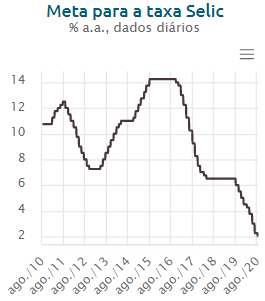
\includegraphics[width=.60\linewidth]{financeira-professor13}
\end{figure}

\begin{figure}[H]
\centering

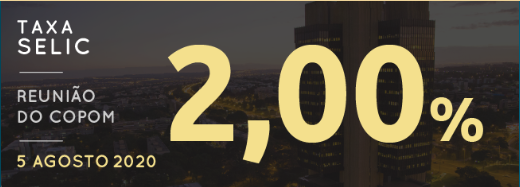
\includegraphics[width=.6\linewidth]{financeira-professor12}
\end{figure}


Temos as taxas de juros em relação ao crédito nas mais variadas modalidades. Temos as taxas de juros pagas pelos investimentos, tais como poupança, títulos do tesouro, fundos imobiliários, renda variável, etc.

Uma pequena pesquis  no site do Banco Central nos mostra a variedade de taxas de juros cobradas para os diferentes tipos de crédito no Brasil.

\begin{figure}[H]
\centering

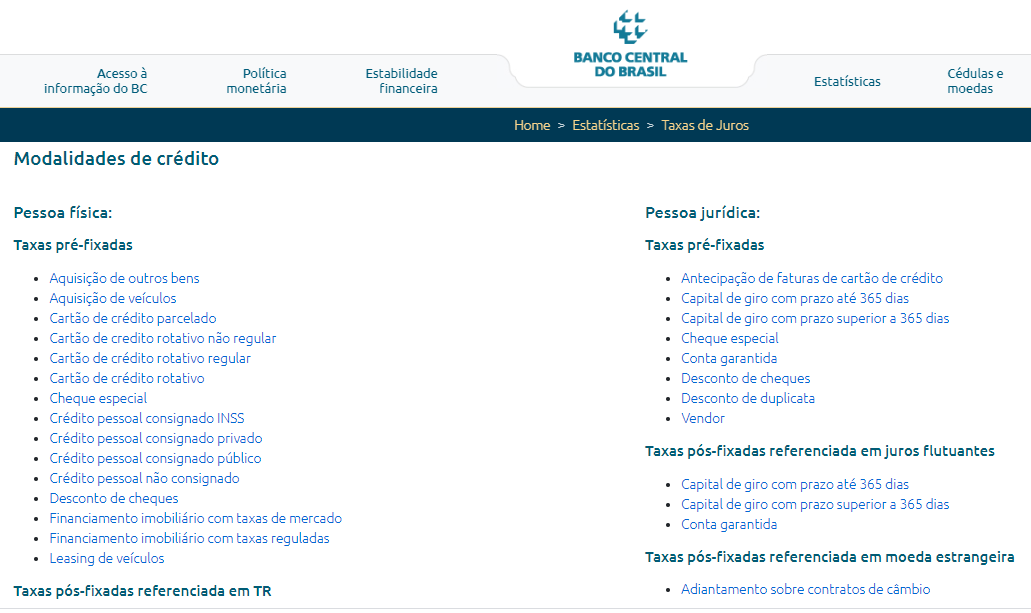
\includegraphics[width=\linewidth]{financeira-professor14}

\caption{Fonte: \href{https://www.bcb.gov.br/estatisticas/txjuros}{Banco Central do Brasil}}
\end{figure}

Por que é tão elevada a taxa de juros no Brasil, em especial o crédito para pessoa física?

Não há consenso entre os economistas sobre as respostas para essa pergunta. Cada economista apresenta sua visão, conforme podemos verno artigo de \cite{BARBOZA2015}, que é refutada ou questionada por outros economistas. Vejamos algumas explicações.

\begin{itemize}
  \item Manter a inflação numa meta estabelecida, reduzir demanda para controlar a inflação, limitar a desvalorização cambial para evitar inflação de custos, induzir investidores a comprarem dívida pública \citep{bresser2002}.

  \item Incerteza jurisdicional, que é a dificuldade de determinar o nível de estabilidade e segurança dos contratos firmados nas leis de uma determinada jurisdição \citep{arida2004}, o que é contestado por \cite{gonccalves2007}.

  \item Segmentação do mercado de crédito \citep{BARBOZA2015}.

  \item Baixa penetração do crédito livre dentro do processo de determinação de renda.

  \item Alto nível da dívida pública \citep{favero2002}, o que é questionado por \cite{muinhos2006}.

  \item  Coalização de interesses formada em torno da manutenção dos juros em níveis elevados \citep{erber2008}.

  \item taxa de impaciência do brasileiro \citep{Barros2011}, o que é contestado por \cite{Schwartsman2011}.

  \item Alta inflação de serviços, por ser um setor com menor elasticidade da oferta, o que é refutado por \cite{Baumol2012}, que mostra que outros países que têm alta inflação no setor de serviços não têm a mesma taxa de juros do Brasil.
\end{itemize}

Alguns termos são bem técnicos, e é claro que o professor de Matmática não precisa se apropriar de todos eles para abordar o tema.

Entretanto, é importante que o professor entenda que o problema das altas taxas de juros no Brasil existe, ele é complexo, as exmplicações não são simples, não há consenso entre os economistas, essa realidade influencia a vida de toda a população, e tem consequências consequências cruéis na vida das famílias menos abastadas, que podem ser as famílias de seus alunos.

Indo além, o professor pode ter um papel muito importante para ensinar o seu aluno a tentar se proteger de determinadas armadilhas dos juros, para tentar não aceitar determinadas taxas quando possível. Ele pode ajudar seus alunos a construir a cultura do cuidado com os juros, pesquisando o crédito, identificando distorções e comparando opções, e não aceitando abusos, quando possível é uma das funções mais importantes da Educação Financeira.

\end{paginatexto}

\def\currentcolor{session1}



\explore{Taxas de Juros no Cenário Brasileiro}
\label{fin-exp-6}

Quando o assunto é taxa de juro, o cenário brasileiro, em  especial, aquel que pagamos quando pegamos emprestado para a realização de algum sonho de médio a longo prazo ou para empreender em algum negócio, bem como nos ajudar em alguma emergência, o cenário brasileiro ainda é extremamente desafiador. As taxas cobradas, em diversas modalidades de crédito, são exorbitantes quando comparadas aos países da América Latina, da Europa e de outros lugares do mundo. A imagem a seguir apresenta apenas um exemplo dessa catástrofe econômica brasileira.

\begin{figure}[H]
\centering

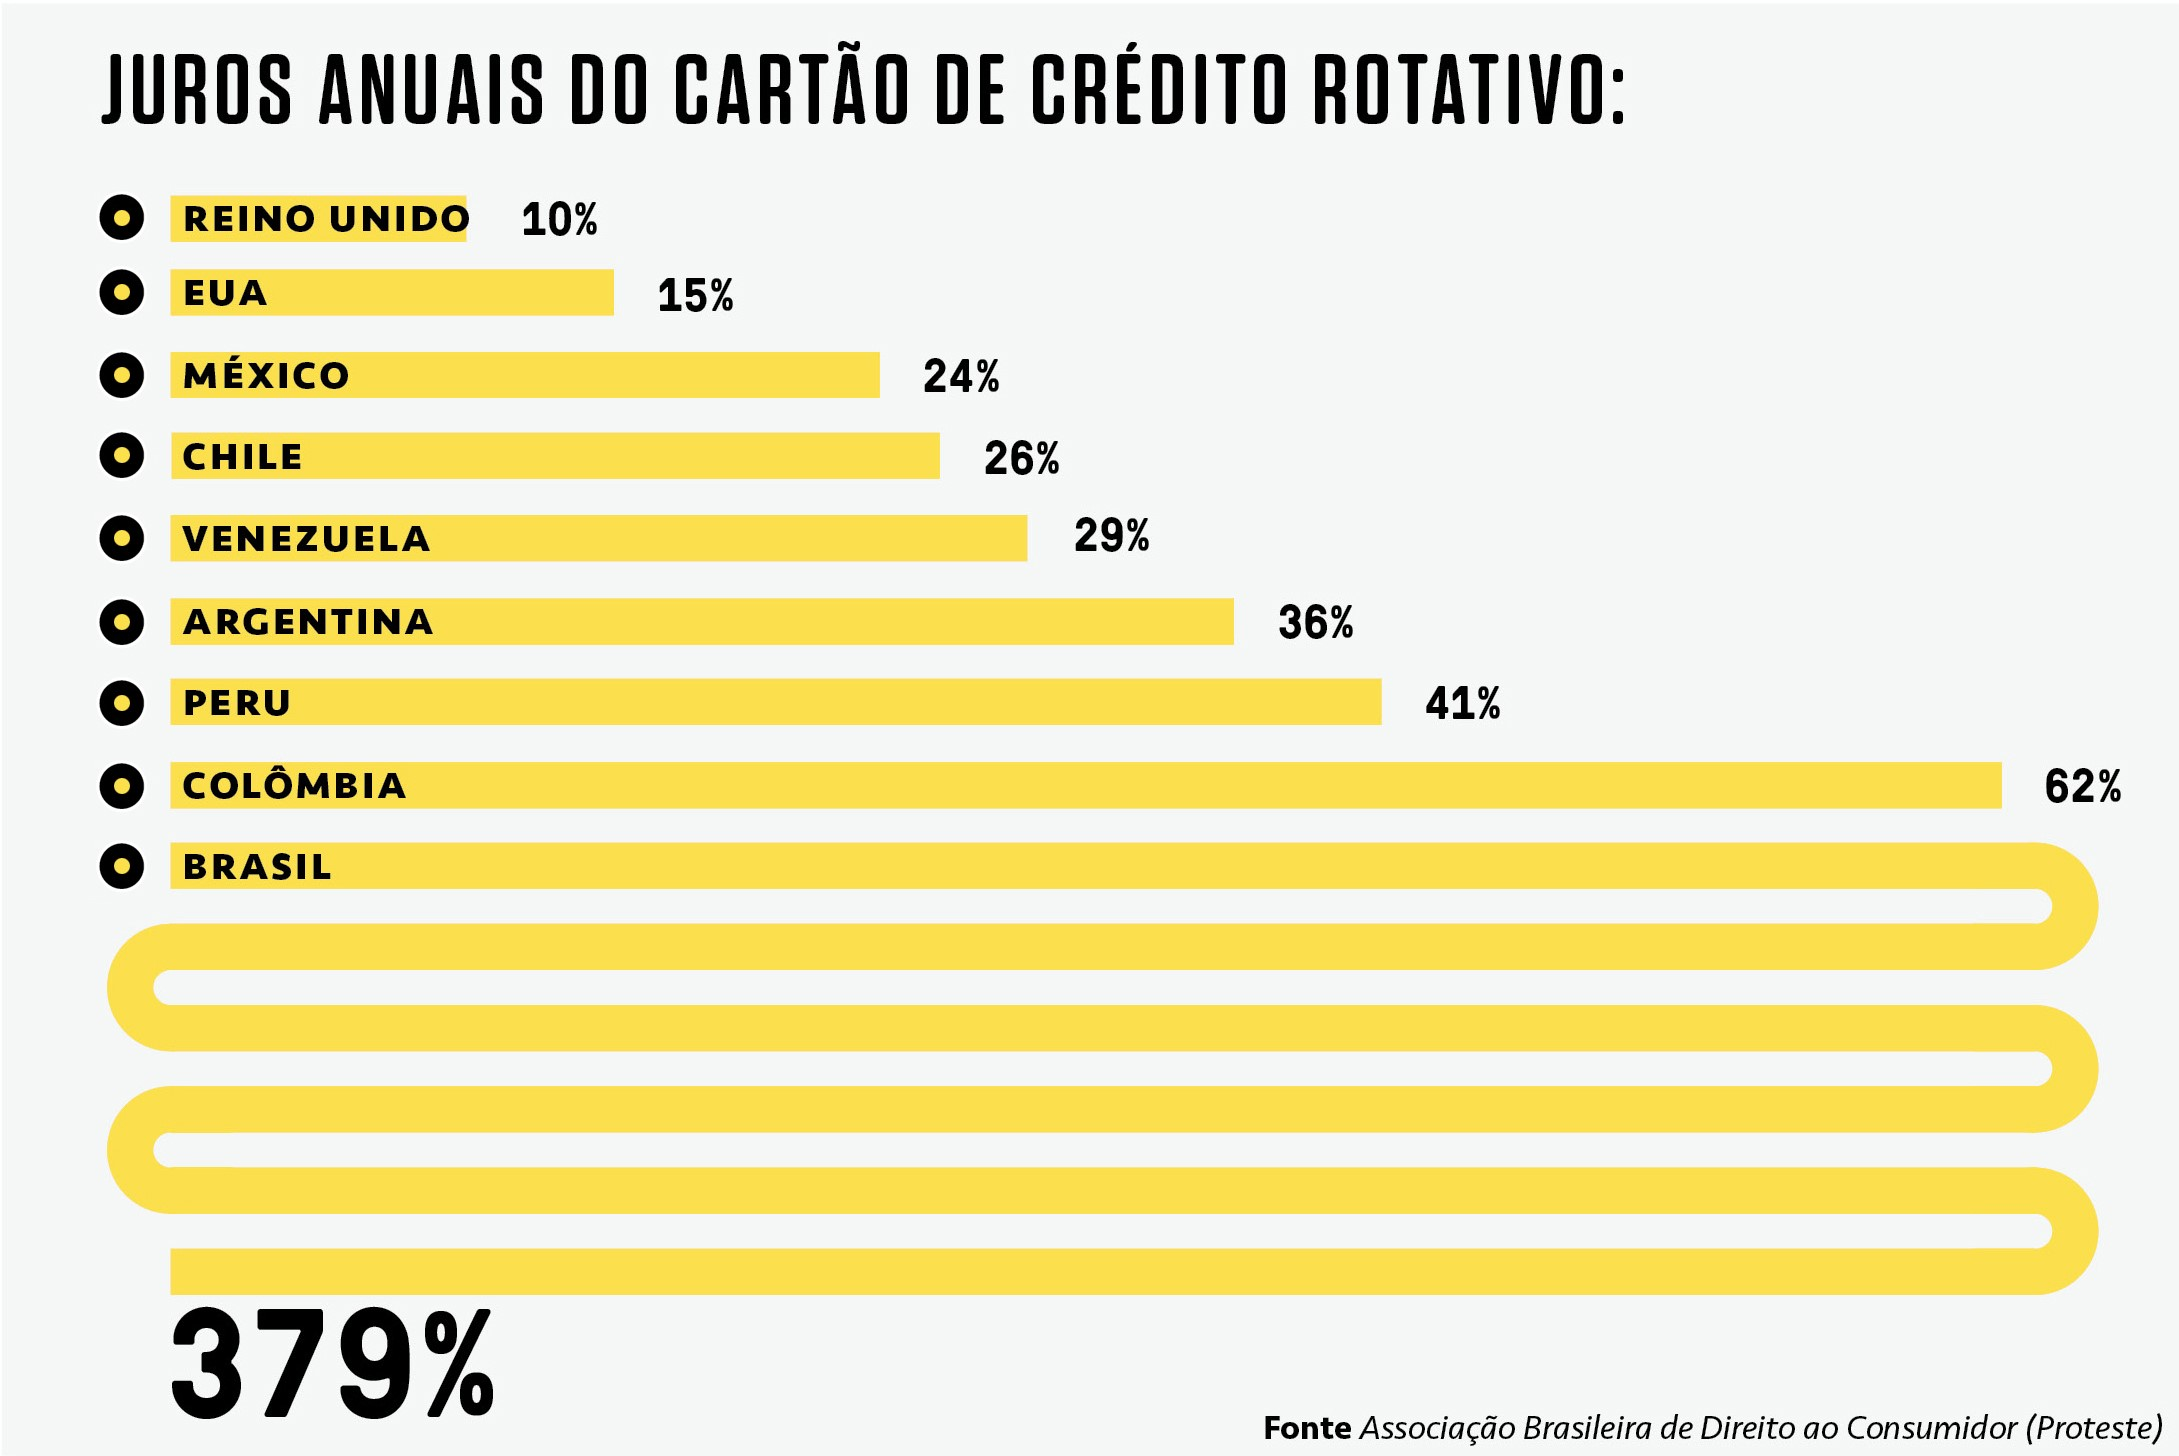
\includegraphics[width=350bp]{financeira15}
\end{figure}


\textbf{Mas o que as taxas de juros praticadas no Brasil têm a ver com a vida do cidadão comum? Por que eu preciso aprender sobre taxas de juros e de que maneira isso afetará a minha vida?}

A resposta: tudo! Para responder à segunda pergunta, convidamos você a investigar e refletir com a gente como essas taxas podemo destruir sonhos e oportunidades de uma vida melhor de milhões de pessoas todos os dias, e de como você pode utilizar com inteligência e sabedoria algumas oportunidades para realizar teus sonhos e projetos.

Você será convidado a aprender sobre taxas para tentar se proteger de determinadas armadilhas, para tentar não aceitar determinadas práticas, e para construir a cultura do cuidado com os juros, pesquisando o crédito, identificando distorções e comparando opções.

Você quer entender como? Então venha conosco para mais uma viagem na incrível, e muitas vezes assustador, mundo das taxas.

O Banco Central do Brasil disponibiliza em seu portal uma gama de taxas de juro cobradas pelos principais bancos brasileiros, em diferentes modalidades de crédito, bem como para diferentes tipos de pessoas (FÍSICAS E JURÍDICAS). A atividade a seguir convida o leitor a refletir sobre esse tema tão importante para uma educação financeira crítica, que ofereça elementos de reflexão e atitude para uma vida melhor. 
\clearpage
\begin{objectives}{Velozes e Furiosos! Uma conversa sobre taxas equivalentes}
{
\begin{itemize}
\item Investigar situações financeiras que envolvam o valor do dinheiro no tempo, considerando taxas proporcionais ou equivalentes
\item Resolver problemas relacionados às taxas proporcionais ou equivalentes.
\item Analisar e tomar decisões em situações econômico-financeiras que envolvam o valor do dinheiro no tempo, considerando aspectos matemáticos e não matemáticos.
\end{itemize}
}{1}{2}
\end{objectives}
\begin{sugestions}{Velozes e Furiosos! Uma conversa sobre taxas equivalentes}
{
Nessa atividade, baseado em taxas reais (de set 2019), disponíveis no site do Banco Central, convidamos o aluno pensar sobre a situação das taxas de juros no Brasil, em especial às taxas que nos cobram. E para isso, entender o conceito de equivalência de taxas pode ser muito importante. Escolhemos para essa atividade as taxas de juro do crédito rotativo do Cartão de Crédito por ser uma das maiores aberrações da realidade econômica Brasileira. E algo que costuma atormentar a vida de milhões de Brasileiros segundo dados do Serasa Experian. 

Tenha em mente que os modelos exponenciais ajudam a compreender taxas equivalentes e calculá-las. Mas elas podem ser abordadas já no ensino fundamental (9º ano por exemplo), com auxílio de calculadoras e/ou planilhas, usando processos multiplicativos apenas. Usar aplicativos de celulares também podem ser um bom caminho, tendo sempre o cuidado de convidar o estudante a entender os processos, e a estabelecer relações funcionais. 

Aproveite essa oportunidade para discutir os processos aditivos e multiplicativos envolvidos na apresentação e cálculo dessas taxas, e como nosso cérebro tende a sobrepor o pensamento aditivo sobre o multiplicativo. 

Finalmente, perceba que ricos e pobres tomam dinheiro emprestado, sendo que os objetivos geralmente são diferentes. E que o crédito está diretamente associado às taxas equivalentes, pois são uma medida rápida de comparação de custo desse crédito, e muitas vezes usada para tomar decisão financeira. 

Finalmente, registramos que esse tema influencia a vida de amplo espectro da sociedade brasileira, o que reforça e justifica sua abordagem no Ensino Médio. 

}{1}{2}
\end{sugestions}
\begin{answer}{Velozes e Furiosos! Uma conversa sobre taxas equivalentes}
{
A atividade será discutida e resolvida na próxima seção.
}{1}
\end{answer}

\begin{task}{Velozes e Furiosos! Uma conversa sobre taxas equivalentes}
\label{fin-ativ-24}

\begin{table}[H]
\centering

\begin{tabular} {|c|l|c|c|}
\hline
\tmcol{2}{|c|}{} & \tmcol{2}{c|}{Taxas de juros} \\
\hline
\tcolor{Posição} & \tmcol{1}{c|}{Instituição} & \tcolor{\% a.m.} & \tcolor{\% a.a}\\
\hline
1 & BCO BMG S.A. & 3,91 & 58,41 \\
\hline
2 & BCO OLÉ BONSUCESSO CONSIGNADO S.A. & 4,33 & 66,27 \\
\hline
3 & BCO DAYCOVAL S.A. & 4,77 & 74,90 \\
\hline
4 & BANCO INTER & 4,86 & 76,68 \\
\hline
5 & BCO INDUSTRIAL DO BRASIL S.A. & 5,70 & 94,55 \\
\hline
6 & BCO BRADESCO S.A. & 8,35 & 161,79 \\
\hline
7 & BANCOOB & 8,64 & 170,32 \\
\hline
8 & BCO C6 S.A. & 8,96 & 179,90 \\
\hline
9 & BCO DO NORDESTE DO BRASIL S.A. & 8,96 & 179,92 \\
\hline
10 & BCO DO BRASIL S.A. & 9,50 & 197,92 \\
\hline
11 & CARUANA SCFI & 10,23 & 221,97 \\
\hline
12 & CAIXA ECONOMICA FEDERAL & 10,38 & 227{,}00 \\
\hline
13 & BCO BNESTES S.A. & 10,77 & 241,21 \\
\hline
14 & BCO ITAUCARD X.A. & 10,99 & 249,61 \\
\hline
\end{tabular}

\caption{Fonte: Banco Central, acesso em 02/09/2019}
\end{table}

Se um ano tem 12 meses, explique por que uma taxa de aproximadamente $11$\% ao mês, cobrada pelo último Banco da lista apresentada na figura, NÃO é equivalente a $12\times11$\% = $132$\% ao ano, e sim a $250$\% ao ano?

Quanto tempo leva para uma pessoa ter sua dívida duplicada, se ela ficar devendo o rotativo do cartão de crédito do último Banco da lista apresentada?

E quanto tempo leva para uma pessoa dobrar um capital, se ela investir na poupança? (6\% ao ano aproximadamente)
\end{task}

\arrange{Taxas de Juros no Cenário Brasileiro}
\label{fin-arg-6}

Duas taxas são equivalentes quando, aplicadas a uma mesma quantia, produzem o mesmo valor futuro em um mesmo período.

Assim, ao aplicar um capital de 100 reais a uma taxa de $1$\% ao mês, quantos por cento ele crescerá em um ano?

Em um ano, $\mathit{VF} = 100\times 1{,}01^{12} = 112{,}68$ reais. Logo a taxa anual é de 12,68\%. \textbf{$\bm{1}$\% ao mês é equivalente a $\bm{12,68}$\% ao ano}.

De um modo geral, uma quantia $C$, aplicada a uma taxa $i$ ao período, durante $n$ períodos, transformar-se-á em um valor futuro igual a 

$$\mathit{VF}=C(1+1)^n$$

Ao mesmo tempo, se aplicar a uma taxa $I$ ao período de $n$ mesesm, transformar-se-á em:

$$\mathit{VF}=C(1+I)$$

Logo, temos a seguinte relação entre duas taxas equivalentes:

$$(1+I)=C(1+i)^n$$

Ou seja, para obter a taxa anual equivalente a 1\%ao mês, bastaria fazer
$$I=(1+1\%)^{12}-1=12{,}68\% \text{ ao ano}$$

Para finalizar, é importante entender duas coisas em relação às taxas de juro. A primeira é que não basta entender a equivalência de taxas, é preciso ter atitude responsável em relação a elas. Conhecimento sem atitude não gera resultados. Se limitar à compreensão do modelo matemático que a representa pode não ser o suficiente para que você entenda e aproveite oportunidades, bem como possa tentar fugir de armadilhas.

Vamos começar pensando nas oportunidades. Por exemplo, aumentar a taxa de retorno de seus investimentos para a aposentadoria de $0{,}5$\% para $0{,}7$\% aos mês, por exemplo, pode gerar, no longo prazo, uma grande diferença. Em 20 anos, por exemplo, na primeira taxa ter-se-ia um retorno de $231$\% e para a segunda taxa $433$\%. No longo prazo, essa diferença de $0{,}2$\% produzirá uma grande diferença entre as rentabilidades totais. Se uma pessoa aplicou 10.000 reais, terá 33.100 na primeira e 53.000 reais na segunda. Mas se a aplicação for de 100 reals, passamoss de 331 mil reais para 533 mil reais. 

\textbf{Isso mesmo! Se a aplicação for de $100$ mil reais, passamos de $331$ mil reais para $533$ mil reais. Veja que $0{,}2$\% pode gerar uma diferença bem significativa entre os valores acumulados.}

O quadro a seguir mostra uma simulação para algumas taxas mensais de retorno, considerando um intervalo discreto de 10 a 30 anos, com variação de 5 anos.

\begin{table}[H]
\centering
% \newcommand{\gline}{\rowcolor{secundario!20}}
\begin{tabular}{|c|c|c|c|c|c|}
\hline
\tcolor{Rentabilidade} & \tmcol{5}{c|}{Tempo de aplicação (em anos)} \\
\hline
Mensal & 10 & 15 & 20 & 25 & 30 \\
\hline
0,10\% & 12,74\% & 19,71\% & 27,11\% & 34,97\% & 43,31\% \\
\hline
0,20\% & 27,09\% & 43,28\% & 61,53\% & 82,10\% & 105,30\% \\
\hline
0,30\% & 43,26\% & 71,46\% & 105,22\% &  145,63\% & 193,99\% \\
\hline
0,40\% & 61,45\% & 105,15\% & 160,67\% & 231,22\% & 320,86\% \\
\hline
0,50\% & 81,94\% & 145,51\% & 231,02\% & 346,50\% & 502,26\% \\
\hline
0,60\% & 105{,}00\% & 193,52\% & 320,26\% & 501,72\% & 761,54\% \\
\hline
0,70\% & 130,95\% & 251{,}00\% & 433,42\% & 710,66\% & 1132{,}00\% \\
\hline
0,80\% & 160,17\% & 319,66\% & 576,90\% & 991,84\% & 1661,13\% \\
\hline
0,90\% & 193,05\% & 401,66\% & 758,78\% & 1370,11\% & 2416,63\% \\
\hline
1{,}00\% & 230,04\% & 499,58\% & 989,26\% & 1878,85\% & 3494,96\% \\
\hline
1,50\% & 496,93\% & 1358,44\% & 3463,28\% & 8605,88\% & 21170,38\% \\
\hline
2{,}00\% & 976,52\% & 3432,08\% & 11488,87\% & 37923,45\% & 124656,11\% \\
\hline
\end{tabular}
\end{table}



\textbf{Que tal fazer uma simulação para outros valores de taxas e outros prazos usando planilhas eletrônicas?}

Passemos agora para as armadilhas. Se uma pessoa se acostuma a usar o cheque especial durante um ano, pagando taxas de $8$\% a $10$\% ao mês (valores do primeiro semestre de 200 no Brasil), em vez de se organizar financeira mente para não precisar fazer isso, ou caso seja realmente necessário o empréstimo, fazê-lo a uma taxa menor, ele estará adiando alguns sonhos, deixando de ter alguns bens, reduzindo a possibilidade de ajudar outras pessoas, a empreender novos aminhos. Não prestar atenção às taxas pode adiar o futuro, ou até mesmo, torná-lo impossível

A segunda coisa mais importante é que, quanto mais informação, mais perdidos podemos ficar. No Brasil, existem diversas taxas de juros em relação ao crédito, que mudam bruscamente dependendo do objetivo do crédito e da instituição financeira que a oferece. Existem ainda muitas modalidades de crédito. Temos as taxas de juro pagas pelos investimentos, tais como poupança, títulos do tesour, fundos imobiliários, renda variável, etc.

\textbf{Uma pequena pesquisa no site do Banco Central nos mostra a variedade de taxas de juros cobradas para os diferentes tipos de crédito no Brasil.}

\begin{figure}[H]
\centering

\fbox{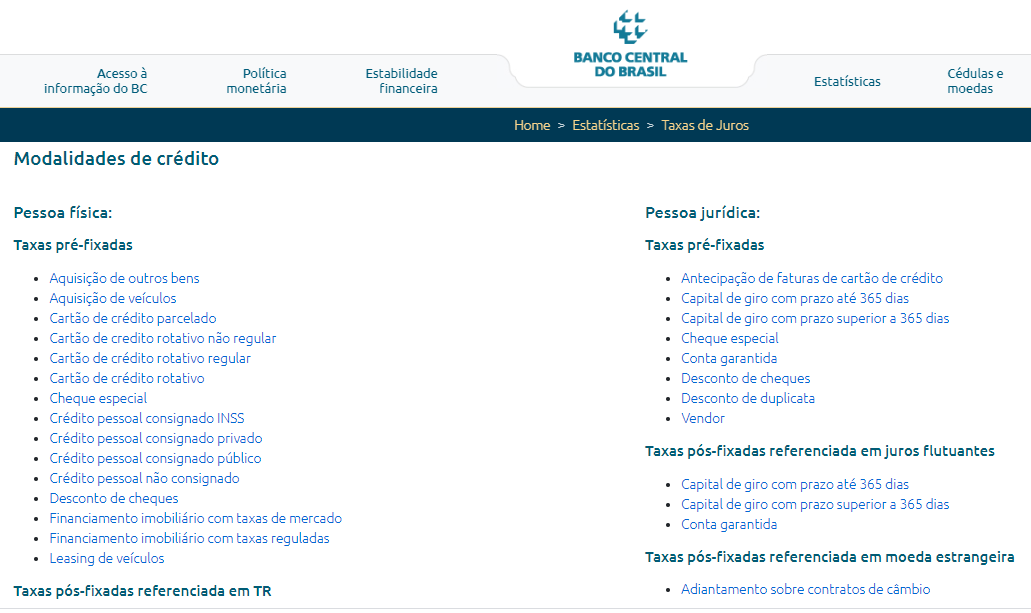
\includegraphics[width=450bp]{financeira17}}
\end{figure}

Então, procure se planejar para avaliar se, e quando, vai tomar crédito, para escolher o tipo de crdito mais adequado para você, pesquisando bem as taxas, e negociando valores sempre que possível.

Lembre-se que as taxas que nos cobram são geralmente maiores que as taxas que nos paga.

\clearpage

\def\currentcolor{session2}

\begin{objectives}{Imprevistos e Cheque especial: uma dupla explosiva}
{
\begin{itemize}
\item Investigar situações financeiras que envolvam o valor do dinheiro no tempo, considerando taxas proporcionais ou equivalentes
\item Resolver problemas relacionados às taxas proporcionais ou equivalentes.
\item Analisar e tomar decisões em situações econômico-financeiras que envolvam o valor do dinheiro no tempo, considerando aspectos matemáticos e não matemáticos.
\end{itemize}
}{1}{2}
\end{objectives}
\begin{sugestions}{Imprevistos e Cheque especial: uma dupla explosiva}
{
Nessa atividade, convidamos o aluno a tomar decisões diante de uma situação de emergência, mas agora olhando para as taxas das opções que têm. Inserimos os valores tanto para criar uma possibilidade para o cálculo das taxas equivalentes como para retomar o conceito de juros compostos abordado anteriormente. 

Não colocar a taxa do cheque especial foi proposital, pois deixar isso aberto vai exigir que o aluno perceba a necessidade dessa informação, e daí empreender uma busca por ela. Também temos a intenção com isso, de que a atividade possa ser realizada com os dados atualizadas no momento de aplicação dela. Com isso, o gabarito é claro se altera, mas o aluno ganha na pesquisa, na investigação e na sensação de realidade ao trabalhar com dados atualizados. 
Os dois dias foram inseridos para representar a emergência da situação, e tirando isso, podem ser ignorados para todo o resto.

}{1}{2}
\end{sugestions}

\begin{objectives}{Reduzindo taxas e ampliando oportunidades}
{
\begin{itemize}
\item Investigar situações financeiras que envolvam o valor do dinheiro no tempo, considerando taxas proporcionais ou equivalentes
\item Resolver problemas relacionados às taxas proporcionais ou equivalentes.
\item Analisar e tomar decisões em situações econômico-financeiras que envolvam o valor do dinheiro no tempo, considerando aspectos matemáticos e não matemáticos.
\end{itemize}
}{1}{2}
\end{objectives}
\begin{sugestions}{Reduzindo taxas e ampliando oportunidades}
{
Nessa atividade, convidamos o aluno a investigar como pequenas reduções em taxas mensais podem gerar grandes reduções em taxas equivalentes em prazos maiores. Mais do que um problema sobre a conversão de taxa mensal para anual, ou seja, de equivalência de taxas, essa situação financeira pode ser usada como um convite a pensar como a redução de taxa de juro cobrada das pessoas pode gerar grandes oportunidades. Juros pagos podem ser sonhos adiados. Juros pagos podem ser desejos destruídos.

Na medida que a população tenta lutar contra esse sistema de juros altos, se planejando para tentar não recorrer a eles, ela tende a força a queda dos juros. Crédito aqui pode funcionar como um produto qualquer: se a demanda diminui então o preço do crédito tende a cair também. E uma população que tenta pensar e agir assim, pode colher os frutos de um crédito mais barato.
\columnbreak
}{0}{2}
\end{sugestions}
\begin{answer}{Imprevistos e Cheque especial: uma dupla explosiva}
{
\begin{enumerate}
\item A estratégia mais eficiente seria Cláudia utilizar o dinheiro da poupança, pois não pagaria juros no empréstimo

Outro caminho é comparar a sua taxa de retorno ($0{,}6\%$ a.m.) com a taxa de juro do empréstimo (em set/2020, por exemplo, a taxa do cheque especial estava em $7{,}54\%$ ao mês (bem maior que $0{,}6\%$ a.m.), conforme mostra o quadro a seguir. 

Veja que basta comparar as taxas para tomar uma decisão mais favorável do ponto de vista \textbf{exclusivamente financeiro}.

\begin{table}[H]
\textbf{Período}: 21/08/2020 a 27/08/2020

\textbf{Modalidade}: Pessoa física - Cheque especial

\textbf{Tipo de encargo}: Pré-fixado
\vspace{1em}

\centering
\begin{tabular} {|c|l|f|f|}
\hline
\tmcol{2}{|c|}{} & \tmcol{2}{c|}{Taxas de juros} \\
\hline
\tcolor{Posição} & \tmcol{1}{c|}{Instituição} & \tmat{\%} $\tcolor{a.m.}$ & \tmat{\%} $\tcolor{a.a}$\\
\hline
1 & BCO RIBEIRAO PRETO S.A. & 0{,}91 & 11{,}50 \\
\hline
2 & BCO CREFISA S.A. & 1{,}45 & 18{,}89 \\
\hline
3 & BCO ALFA S.A. & 1{,}80 & 23{,}89 \\
\hline
4 & BCO SOFISA S.A. & 2{,}24 & 30{,}45 \\
\hline
\hline
13 & BANCO INTER & 6{,}00 & 101{,}20 \\
\hline
14 & BCO DO EST. DO PA S.A. & 6{,}01 & 101,48 \\
\hline
15 & BCO DAYCOVAL S.A. & 6{,}77 & 119{,}44 \\
\hline
16 & BCO C6 S.A. & 7{,}48 & 137{,}71 \\
\hline
17 & BCO DO BRASIL S.A. & 7{,}54 & 138{,}27 \\
\hline
\end{tabular}
\end{table}

\item Os R\$ $5.000$ se aplicados na poupança a uma taxa de $0{,}5$\% durante 6 meses daria o valor de R\$ $5.182{,}72$

Por outro lado, tomando dinheiro emprestado a $7{,}5\%$ ao mês (Banco do Brasil em Set/2020), em 6 meses ela pagaria de Juros:
\begin{align*}
J&=5.000\times(1+7{,}5\%)^6-5.000\\
J&=\text{R\$ }2.716{,}51
\end{align*}

Para fins de comparar taxas, e tomar decisão sobre a opção com menor perda financeira, também poderíamos usar apenas a equivalência de taxas. Chamando de $I_1$ e $I_2$ as taxas de retorno da poupanção e de juro do cheque especial, equivalentes às respectivas taxas mensais dadas, temos:
\begin{align*}
I_1&=(1+0{,}6\%)^6-1=3{,}65\%\text{ ao semestre}\\
I_1&=(1+7{,}5\%)^6-1=3{,}54{,}33\%\text{ ao semestre}
\end{align*}

Para responder ao item \titem{b)}, temos o seguinte quadro.

Se ela deixar o dinheiro na poupança, ao final de seis meses ela ganhará R\$ $182{,}72$ pela aplicação, mas perderá (pagando de juros) R\$ $2.716{,}51$, gerando uma perda líquida de R\$ $2533{,}79$.

Se ela usar o dinheiro na poupança para emergência e não tomar dinheiro emprestado no cheque especial, ao final de seis meses ela terá uma perda líquida de R\$ $182{,}72$, pois não terá pago nada de juros.

A diferença, dadas as taxas absurdas cobradas no Brasil, também é absurda. Isso reforça a importância do tema e do cuidado que as pessoas devem ter com o uso do cheque especial (muito fácil de usar pois está disponível a qualquer momento).
\end{enumerate}.


\tcbsubtitle{Reduzindo taxas e ampliando oportunidades}
Primeiro temos que transformar a taxa $2{,}99$\% a.a. para uma taxa anual, taí temos $(1+0{,}0299)^{12}=1+i_{\text{anual}}$, resolvendo esta equação, temos $i_{\text{mensal}}=0{,}4241=42{,}41$\%. Agora temos que transformar $2{,}29$\% a.am. para uma taxa anual, daí temos $(1+0{,}0299)^{12}=1+i_{\text{anual}}$. A redução, em pontos percentuais será $42{,}41\%-31{,}22\%=11{,}19\%$. 

}{9}
\end{answer}
\begin{objectives}{Velozes e Furiosos 2 - As taxas atacam novamente}
{
\begin{itemize}
\item Investigar situações financeiras que envolvam o valor do dinheiro no tempo, considerando taxas proporcionais ou equivalentes
\item Resolver problemas relacionados às taxas proporcionais ou equivalentes.
\item Analisar e tomar decisões em situações econômico-financeiras que envolvam o valor do dinheiro no tempo, considerando aspectos matemáticos e não matemáticos.
\end{itemize}
}{1}{1}
\end{objectives}
\begin{sugestions}{Velozes e Furiosos 2 - As taxas atacam novamente}
{
Nessa atividade, convidamos o aluno a investigar o custo do crédito em diferentes opções, comparando o cheque especial com o rotativo do cartão de credito e o consignado. Recomendamos que o professor peça aos alunos para pesquisarem os custos dessas diferentes modalidades, incluindo as que atualmente são usadas pela família, se for o caso. O site do Banco central tem uma parte exclusiva sobre taxas de juro, quinzenalmente atualizadas, e disponível em \url{https://www.bcb.gov.br/estatisticas/txjuros}
}{1}{1}
\end{sugestions}
\begin{answer}{Velozes e Furiosos 2 - As taxas atacam novamente}
{
  \begin{enumerate}
    \item Modalidade de Crádito Consignado: Esta é uma modalidade de empréstimo destinada somente para as pessoas aposentadas e/ou pensionistas INSS, militares das forças armadas, trabalhadores assalariados de empresas privadas e servidores públicos. É importante dizer que as parcelas do empréstimo nessa modalidade são deduzidas diretamente de folha de pagamento ou benefício da pessoa física.

    Modalidade de Crédito de Cheque Especial: Esta é uma modalidade de empréstimo pré-aprovado pelo banco para o correntista (pessoa que possui conta corrente no banco).

    Modalidade de Crédito no Cartão de Crédito Rotativo: Quando o consumidor não faz o pagamento total da fatura do cartão dfe crédito até o seu vencimento, este crédito é oferecido. O termo rotativo acontece quando o consumidor efetua qualquer pagamento menor que o valor total da fatura do cartão de crédito.

    \item A primeira modalidade é mais barata que as outras devido a esse público de pessoas possuírem uma garantia de uma renda mensal (salário), ouseja, as chances dessas pessoas não terem dinheiro para honrar o empréstimo com o banco é baixa.

    \item Resposta pessoal.
  \end{enumerate}
}{0}
\end{answer}
\begin{objectives}{Crédito pessoal é sinônimo de dívida?}
{
\begin{itemize}
\item Investigar situações financeiras que envolvam o valor do dinheiro no tempo, considerando taxas proporcionais ou equivalentes
\item Resolver problemas relacionados às taxas proporcionais ou equivalentes.
\item Analisar e tomar decisões em situações econômico-financeiras que envolvam o valor do dinheiro no tempo, considerando aspectos matemáticos e não matemáticos, em especial às envolvendo o custo do crédito e sua facilidade de acesso.
\end{itemize}
}{1}{1}
\end{objectives}
\begin{sugestions}{Crédito pessoal é sinônimo de dívida?}
{Nessa atividade, convidamos o aluno a pensar sobre o custo e facilidade do crédito a partir de um texto bem provocativo. O trecho abaixo é um exemplo da reflexão a que a atividade nos convida.

\begin{quote}
Nos últimos anos fomos envolvidos por grandes campanhas que ofereciam crédito quase que como frutas ou legumes que encontramos nas feiras livres. Bastava escolher a “melhor banca” e o “melhor produto”, mas com um diferencial: pagamentos a perder de vista. A estratégia arriscada não é nova e a prática comprovou que se trata de um tiro no pé do consumidor – ele se satisfaz momentaneamente e cria (muitos) problemas para o futuro.
\end{quote}

Retomamos a discussão sobre o rotativo do cartão de crédito, pois as facilidades de uso do cartão de crédito acompanhadas de uma falta de controle, podem gerar o uso desnecessário desse tipo de crédito. Ele é fácil, mas é muito caro. Gastar mais do que se pode pagar também é algo fácil de acontecer, principalmente quando vivemos tempos de crise, ou de euforia generalizada. No primeiro temos necessidades básicas a serem atendidas. No segundo temos necessidades de termos o luxo que às vezes não podemos ter, ou status que nunca precisaríamos ter.

Independente da motivação e das justificativas, a questão sempre é complexa, pois sempre passa por uma decisão: o que é que tem mais valor pra mim naquele momento? Ou quais são as opções que eu tenho disponíveis naquele momento?

Entender o custo do dinheiro fácil, e como pode ser difícil e doloroso pagar por esse dinheiro que não se tem, talvez possa ajudar as pessoas no planejamento do consumo baseado na capacidade financeira pessoal e familiar.

}{1}{2}
\end{sugestions}
\begin{answer}{Crédito pessoal é sinônimo de dívida?}
{
\begin{enumerate}
\item Resposta individual.
\item Crédito fácil são os produtos de empréstimos oferecidos pelo banco ou instituições financeiras para os consumidores, muitas vezes sem muita burocracia e complexidade em termos do cliente ter que comprovar que possui algum tipo de renda para honrar o compromisso do pagamento do empréstimo até a sua quitação.
\item Resposta pessoal.
\end{enumerate}
}{1}
\end{answer}

\practice{Capitais e Taxas Equivalentes}
\label{fin-prac-6}

\begin{task}{Imprevistos e Cheque especial: uma dupla explosiva}
\label{fin-ativ-25}

Claudia, cliente do Banco do Brasil, teve uma emergência e precisa de 5.000 reais para daqui a dois dias. Ela pode usar o cheque especial para fazer um empréstimo nesse valor ou buscar uma alternativa mais barata. Pensando um pouco, ela lembra que tem 5.000 reais na poupança, guardados por ela mesma para alguma emergência. Considere que esse dinheiro na poupança renda 0,6\% ao mês. 

\begin{enumerate}
\item Qual a estratégia mais eficiente, dentre as apresentadas, do ponto de vista exclusivamente financeiro? Justifique sua resposta. 
\item Quantos reais ela economizaria em juros, considerando um empréstimo de 5.000 reais durante 6 meses, na comparação entre as alternativas apresentadas?
\end{enumerate}
\end{task}

\begin{task}{Reduzindo taxas e ampliando oportunidades}
\label{fin-ativ-26}

O Banco Central do Brasil reduziu, em setembro de 2019, a taxa base da Economia (taxa Selic) de 6,0\% ao ano, para 5,5\% ao ano. A figura mostra como alguns Bancos públicos e privados modificaram algumas de suas taxas devido a essa redução da Selic. 

\begin{figure}[H]
\centering
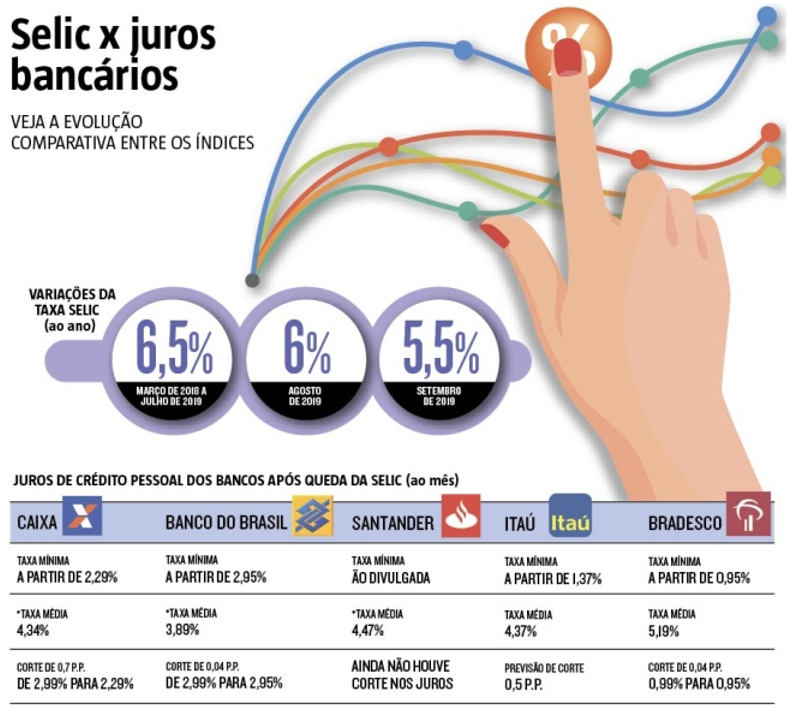
\includegraphics[width=240bp]{selicxjuros.png}

\end{figure}

Considere conforme mostrado na figura que a Caixa Econômica Federal passasse os juros médios do crédito pessoal de 2,99\% a.m. para 2,29\% a.m. Qual seria a redução, em pontos percentuais, da taxa de juro anual cobrada pela Caixa Econômica Federal?
\end{task}


\begin{task}{Velozes e Furiosos 2 - As taxas atacam novamente}
\label{fin-ativ-27}

Leia atentamente os dados a seguir:

\begin{table}[H]
\centering
\begin{tabular}{|c|c|c|c|}
\hhline{~|---|}
\multicolumn{1}{c|}{} & \tcolor{Set/2017} & \tcolor{Out/2017} & \tcolor{Nov/2017} \tabularnewline
\hline
\tcolor{Crédito Consignado}& 3,5\% & 3,4\% & 3,2\% \tabularnewline
\hline
\tcolor{Crédito do Cheque Especial} & 13,0\% & 12,8\% & 12,5\% \tabularnewline
\hline
\tcolor{Crédito do Cartão de Crédito Rotativo} & 15,0\% & 14,6\% & 14,0\% \tabularnewline
\hline
\end{tabular}
\caption{Fonte: Banco Central do Brasil. 2017}
\end{table}


\begin{enumerate}
\item Explique como são cada uma dessas três modalidades de crédito
\item Por que a primeira é muito mais barata que as outras duas?
\item Analisando as imagens a seguir, você acha que o endividamento é bom para as pessoas? E para os Bancos? E para a geração de empregos e crescimento do Brasil?

\begin{figure}[H]
\centering
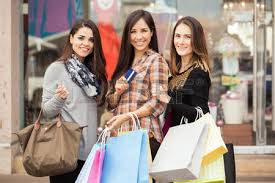
\includegraphics[width=150bp]{compras}
\includegraphics[width=150bp]{compras2}
\includegraphics[width=150bp]{compras3}
\end{figure}
\end{enumerate}
\end{task}



\begin{task}{Crédito pessoal é sinônimo de dívida?}
\label{fin-ativ-28}
\textit{(Texto adaptado do \href{http://www.blogtecnisa.com.br/mercado/credito-pessoal-e-sinonimo-de-divida/}{Blog Tecnisa}) Acesso em Maio de 2014.}

"Nas últimas semanas surgiram ótimas notícias sobre a redução dos juros, promovidos pelo Banco do Brasil e Caixa Econômica Federal que na sequência também foi adotado – em partes – por outros bancos. Mas a redução dos juros não significa que eles ficaram realmente baratos ou que é seja uma sinalização para o consumo sem planejamento.

Se de um lado existe um devedor, de outro lado existe um credor. Muitos tomam emprestados e poucos emprestam – cobrando caro por isso. As pessoas se endividam para adquirir bens ou serviços de que, em uma parte das vezes, não precisam ou não querem (fazem para impressionar) e se deixam vencer pelo apelo da mídia ou pela simples “manutenção do status”.

Falando nisso, uma das definições de status mais brilhante que ouvi nos últimos tempos surgiu no último final de semana, a partir das palavras de um educador financeiro: “Status é o sentimento que move alguém a comprar coisas que não precisa, com o dinheiro que não tem, para agradar alguém que não gosta”. Trata-se da mais pura verdade!

Nos últimos anos fomos envolvidos por grandes campanhas que ofereciam crédito quase que como frutas ou legumes que encontramos nas feiras livres. Bastava escolher a “melhor banca” e o “melhor produto”, mas com um diferencial: pagamentos a perder de vista. A estratégia arriscada não é nova e a prática comprovou que se trata de um tiro no pé do consumidor – ele se satisfaz momentaneamente e cria (muitos) problemas para o futuro.

O velho conto do crédito fácil caiu como uma luva para situação do brasileiro comum, aquele que nunca buscou a educação financeira e o investimento como formas de realização de seus sonhos e objetivos. Provavelmente, isso aconteceu devido à falta de sonhos e objetivos. Aliás, quais são os seus sonhos? Já parou para pensar nisso?

Ao usar o dinheiro fácil oferecido por tantas instituições, o cidadão perceberá, talvez tarde demais, que o pior é o preço desta facilidade. O crédito fácil é caríssimo (mesmo com a redução atual) – sempre foi e sempre será. Devido ao meu envolvimento com o tema, ouço relatos impressionantes de pessoas que hoje não enxergam uma luz ou um caminho para sair desse buraco financeiro.

Sim, a situação pode ficar crítica. São pessoas que vivem a base de remédio, que dizem não ter mais motivo para viver ou que não conseguem nem mesmo comprar alimento para os filhos. A verdade parece distante. Não conte com isso. A realidade está logo ali, na família vizinha, ou mesmo mais perto do que imaginamos – é o nosso amigo, irmão ou nossos pais."


\begin{table}[H]
\centering
\begin{tabular} {|c|l|c|c|}
\hline
\tmcol{2}{|c|}{} & \tmcol{2}{|c|}{Taxas de juros} \\
\hline
\tcolor{Posição} & \tmcol{1}{c|}{Instituição} & \tcolor{\% a.m.} & \tcolor{\% a.a}\\
\hline
1 & BCO BMG S.A. & 3,91 & 58,41 \\
\hline
2 & BCO OLÉ BONSUCESSO CONSIGNADO S.A. & 4,33 & 66,27 \\
\hline
3 & BCO DAYCOVAL S.A. & 4,77 & 74,90 \\
\hline
4 & BANCO INTER & 4,86 & 76,68 \\
\hline
5 & BCO INDUSTRIAL DO BRASIL S.A. & 5,70 & 94,55 \\
\hline
6 & BCO BRADESCO S.A. & 8,35 & 161,79 \\
\hline
7 & BANCOOB & 8,64 & 170,32 \\
\hline
8 & BCO C6 S.A. & 8,96 & 179,90 \\
\hline
9 & BCO DO NORDESTE DO BRASIL S.A. & 8,96 & 179,92 \\
\hline
10 & BCO DO BRASIL S.A. & 9,50 & 197,92 \\
\hline
11 & CARUANA SCFI & 10,23 & 221,97 \\
\hline
12 & CAIXA ECONOMICA FEDERAL & 10,38 & 227{,}00 \\
\hline
13 & BCO BNESTES S.A. & 10,77 & 241,21 \\
\hline
14 & BCO ITAUCARD X.A. & 10,99 & 249,61 \\
\hline
\end{tabular}
\end{table}

\begin{enumerate}

\item Qual a sua opinião sobre o texto?
\item O que é o crédito fácil?
\item Quais são as conexões entre esse texto e a tabela acima, sobre as taxas do rotatifo do cartão de crédito?

\end{enumerate}

\end{task}


\begin{paginatexto}{Inflação e poder de compra}
\subsection*{Objetivo geral}
Investigar situações financeiras que envolvem a noção de inflação, alguns tipos de fatores que a influenciam e possíveis impactos na vida da população.

\textbf{Conceitos abordados}: taxas e fatores; médias; progressão geométrica; inflação (IPCA, IPC IGPM); Efeito Fisher (relação entre inflação e poder de compra), através das habilidades:

\begin{habilities}{EM13MAT101}
 Interpretar situações econômicas, sociais e das Ciências da Natureza
que envolvem a variação de duas grandezas, pela análise dos gráficos das funções representadas e das taxas de variação com ou sem apoio de tecnologias digitais.

\tcbsubtitle{EM13MAT104}

Interpretar taxas e índices de natureza socioeconômica, tais como índice de desenvolvimento humano, taxas de inflação, entre outros, investigando os processos de cálculo desses números.

\tcbsubtitle{EM13MAT203}
Planejar e executar ações envolvendo a criação e a utilização de aplicativos, jogos (digitais ou não), planilhas para o controle de orçamento familiar, simuladores de cálculos de juros compostos, dentre outros, para aplicar conceitos matemáticos e tomar decisões. 

\end{habilities}

\subsection*{Recomendações para o professor}

\paragraph{Organização em sala de aula} Essa seção trata de índices de inflação, que na história do Brasil é algo extremamente importante, pois está diretamente ligado à realização de sonhos e à desigualdade social. Então, convide os estudantes a pesquisarem informações em sites, blogs, jornais, portais, revistas econômicas, sobre situações envolvendo inflação. Convide-os a pesquisar os preços de seu bairro, a identificar a cesta de produtos que consomem, e a criar a cultura de investigar os fundamentos e a razoabilidade das informações veiculadas nas mídias sociais de forma fundamentada.

\paragraph{Dificuldades previstas} Na abordagem dos índices de inflação, geralmente aparecem aumentos sucessivos que geram produtos com números decimais, em especial aqueles que aparecem na média geométrica, e em alguns casos, cálculos envolvendo exponenciais, incluindo as com expoentes fracionários. Essas operações costumam ser consideradas complexas pelos alunos de Ensino Médio, sendo dificuldades previstas na abordagem. Trabalhar com o auxílio de tecnologia pode ajudar a superar tais dificuldades. A variedade de índices de inflação também pode ser pontos de dificuldades e gerar alguns obstáculos iniciais na compreensão das atividades.

\paragraph{Sugestões gerais} Trabalhar com o auxílio de tecnologia pode ajudar a superar tais dificuldades, e acessar o site do Banco Central e do IBGE são ótimas oportunidade para fazer uma imersão no tema. A ideia de inflação pode ser abordada no Ensino Fundamental II, quando se abordam aplicações de porcentagem, por exemplo. Analisar índices sócio-econômicos também faz parte do conjunto de habilidades da BNCC.

\subsection*{Enriquecimento da discussão}

Existem diferentes índices de inflação no Brasil. Abordaremos aqui o Índice de Preços ao Consumidor Amplo (IPCA) e o Índice Geral de preços do Mercado (IGPM). Atualmente, a definição mais comum entre os especialisatas para o termo \textit{inflação de preços} é o aumento continuado e generalizado dos bens e serviços \citep{ecb2017}. Assim, a inflação tem como principal impacto o aumento/redução do poder de compra para o consumidor e para as empresas.

Sugerimos a leitura de pesquisas sobre a abordagem de inflação na Educação Básica nas referências.
\end{paginatexto}


\def\currentcolor{session1}
\begin{texto}
{
  Os objetivos e as discussões seguintes são para o conjunto das quatro atividades desta seção.

  \subsection{Objetivo específicos}
  \begin{itemize}
  \item Investigar situações financeiras que envolvem a noção de inflação, alguns tipos de índices que buscam medir inflação, os fatores que a influenciam e possíveis impactos na vida da população
  \item Resolver problemas relacionados às noções de inflação e poder de compra
  \item Analisar e tomar decisões em situações econômico-financeiras que envolvam a noção de inflação, considerando aspectos matemáticos e não matemáticos.
  \end{itemize}

  \subsection{Sugestões e discussões}

  Nessas quatro atividades disparadoras, convidamos o aluno a pensar sobre situações onde a noção de inflação, poder de compra e ganho real estão presentes. Os aspectos matemáticos aqui são importantíssimos, pois mais uma vez nosso cérebro tende a nos enganar. Um exemplo disso é nos querer empurrar na direção de acreditar que um aumento de $20\%$ na renda, em uma inflação de $5\%$, representa um aumento no poder de compra de $15\%$. Ou seja, temos aqui uma tendência a mobilizar nosso sistema 1, substituindo um problema que não sabemos resolver por outro que sabemos resolver, ou que achamos ser o mesmo problema. Isso gera uma percepção de que o processo aditivo é o adequado para responder a essa situação, quando na verdade não é. E o professor de Matemática, sabendo disso, pode apresentar diferentes situações para mostrar aos alunos por que o processo aditivo não é o mais adequado.

  Na seção organizando as ideias procuramos explicar detalhadamente cada situação, aproveitando para construir e organizar os conceitos nela envolvidos.

  As três primeiras atividades tratam da relação conhecida como Efeito Fisher entre taxa nominal, taxa real e inflação, que será demonstrada no próximo organizando as ideias, que pode ser escrita assim:
  \begin{equation*}
  1+1_{\text{real}}=\frac{1+i_{\text{nominal}}}{1+i_{\text{inflação}}}
  \end{equation*}

  Na terceira atividade convidamos o aluno a entender o principal mecanismo de reajuste dos aluguéis no Brasil: reajuste pelo índice chamado IGPM, que é diferente do principal índice de inflação, que é o IPCA. Esses dois índices são explorados na próxima seção. 

  As atividades "Sua inflação é igual à minha inflação?", "Inflação e investimentos"{} e "Por que o meu aluguel aumento desse jeito?"{} serão apresentadas no Organizando as ideias dessa seção

}
\end{texto}
\clearmargin
\begin{answer}{Cadê o meu dinheiro?}
{
\begin{enumerate}
\item A nota continua sendo de 5 reais, e com ela, compramos produtos cujo preço é de 5 reais, independente do ano.
\item Significa que R\$ $100{,}00$ em 1994 valem apenas R\$ $16{,}65$ em 2019, considerando um determinado tipo de inflação no período. Ou seja, com 100 reais hoje eu consigo comprar hoje apenas o que conseguiria comprar com R\$ $16{,}65$ em 1994. Ou ainda que um produto que custava R\$ $16{,}65$ em 1994 custa hoje R\$ $100{,}00$. 
\item Por causa da redução do poder de compra da moeda, devido a diversos fatores, dentre eles a inflação.
\item A terceira linha apresenta uma inconsistência, derivada de um erro de conta ou digitação, provavelmente, e não de aproximação como podemos perceber no quadro a seguir
\end{enumerate}

}{1}
\end{answer}
\explore{Inflação e Poder de Compra}
\label{fin-exp-7}

Outra situação envolvendo a transformação do dinheiro no tempo se refere à relação entre \textbf{inflação} e \textbf{poder aquisitivo (ou poder de compra)}. O aumento de preços de produtos e serviços interfere diretamente no poder de compra das famílias e na realização de projetos e sonhos das pessoas.

A inflação afeta a vida das pessoas de uma maneira mais forte e sutil do que a maioria imagina ou pensa. Convidamos você a investigar e refletir com a gente esse aspecto econômico tão importante na vida das pessoas, que é a inflação.

Veja as seguintes chamadas de matérias veiculadas nos últimos anos.

\begin{figure}[H]
\centering

\includegraphics[width=450bp]{financeira18}
\end{figure}

Mas o que é inflação? Como é medida? Quais seus impactos no poder de compra das famílias?

Vamos tentar responder a essas perguntas, a partir de quatro atividades.

\begin{task}{Cadê o meu dinheiro?}
\label{fin-ativ-29}
Observe atentamente a imagem a seguir

\begin{figure}[H]
\centering

\includegraphics[width=.3\linewidth]{financeira58}
\end{figure}
\begin{enumerate}
\item O que aconteceu com a nota de R\$ $5{,}00$: continua sendo de $5$ reais ou não?
\item O que significa o valor de R\$ $16{,}65$ sobre a nota de R\$ $100{,}00$ na segunda coluna?
\item Por que o valor das notas na segunda coluna mudou?
\item Você vê algum problema em algum dos valores apresentados na segunda coluna?
\item Qual a relação entre a imagem da figura anterior com o lançamento da nova nota de R\$ $200{,}00$
\end{enumerate}
\begin{figure}[H]
\centering

\includegraphics[width=.5\linewidth]{financeira59}
\end{figure}
\end{task}

\begin{task}{Sua inflação é igual à minha inflação?}
\label{fin-ativ-30}
Considere uma família cuja renda mensal, em janeiro de 2019, seja de R\$ $5.000{,}00$. Vamos supor que a inflação para essa família tenha sido de $10$\% durante esse ano. Isso significa que, em média, os produtos que a família consumia aumentaram $10$\% em um ano. Por outro lado, vamos admitir que a renda da família, em janeiro de 2020, seja $15$\% maior, e que a inflação oficial anunciada tenha sido de $5\%$ ao ano.

Qual foi o aumento do poder de compra dessa família nesse período, considerando a inflação oficial? E considerando a inflação que de fato aconteceu para essa família?
\end{task}

\begin{task}{Inflação e investimento}
\label{fin-ativ-31}
Maria ganhou um aumento de $10$\% em um ano, mas sua inflação foi de $6$\% ao ano. Benedita ganhou um aumento de $5\%$ mas sua inflação foi de $1$\% ao ano. Qual das duas teve o maior ganho real?
\end{task}

\begin{task}{Por que o meu aluguel aumentou desse jeito?}
\label{fin-ativ-32}
\label{fin-ativ-32}

Josimar alugou um apartamento, em fevereiro de 2019, por R\$ $2.400{,}00$, ficando acordado no contrato que a cada 12 meses o valor seria reajustado pelo índice geral de pre''cos do mercado (IGPM) acumulado nos últimos 12 meses. A tabela abaixo mostra o índice acumulado nos primeiros seis meses de 2020.

\begin{table}[H]
\centering
\begin{tabular}{|c|c|>{\centering}m{.15\textwidth}|>{\centering\arraybackslash}m{.15\textwidth}|}
\hline
\tmcol{4}{|c|}{2020}\\
\hline
\tcolor{Mês} & \tcolor{Mensal (\%)} & \tcolor{Acumulado nos últimos 12 meses (\%)} & \tcolor{Acumulado no ano (\%)} \\
\hline
Janeiro & 0,48 & 7,8223 & 0,4800 \\
\hline
Fevereiro & 0,04 & 6,8389 & 0,4398 \\
\hline
Março & 1,24 & 6,8178 & 1,6843 \\
\hline
Abril & 0,80 & 6,6908 & 2,4987 \\
\hline
Maio & 0,28 & 6,5103 & 2,7857 \\
\hline
Junho & 1,56 & 7,3133 & 4,3892 \\
% \hline
% Julho & & & \\
% \hline
% Agosto & & & \\
% \hline
% Setembro & & & \\
% \hline
% Outubro & & & \\
% \hline
% Novembro & & & \\
% \hline
% Dezembro & & & \\
\hline
\end{tabular}
\end{table}

Em março de 2020, ele percebeu que o aluguel passou de R\$ $2.400{,}00$ para R\$ $2.564{,}00$. O valor do aluguel foi reajustado corretamente? Justifique sua resposta
\end{task}

Vamos refletir sobre essas situações econômico-financeiras, investigando cada atividade nopróximo tópico do \textit{Organizando as ideias}

\clearpage
\arrange{Índices de Inflação e Seus Impactos}
\label{fin-arg-7}

Essas atividade ilustram, um pouco, como a inflação pode interferir profundamente na vida das pessoas. 

\subsection{Mas o que é inflação?}

Atualmente, a definição mais comum entre os especialistas para o termo \textit{inflação de preços}, é o aumento continuado e generalizado dos preços dos bens e serviços \citep{ecb2017}. Assim, a inflação tem como principal impacto o aumento/redução do poder de compra para o consumidor e para as empresas.

Ela consiste tecnicamente em um processo de aumento contínuo de generalizado dos preços de uma certa categoria de bens e serviços ofertados em um país. A ideia de ser contínua está associada ao fato de que sua medição ocorre ao longo do tempo sem interrupções. A ideia de generalizado se refere a um conjunto de produtos e serviços (cesta de produtos) para os quais se olha a evolução dos preços.

 Ou seja, se a inflação em determinado mês for de $0{,}5$\%, isso significa que o aumento médio dos preços dessa cesta no período também foi de $0,5$\%. Isso não significa que todos os produtos aumentaram $0{,}5$\%, ou seja, a variação não é uniforme. Um exemplo disso foi o aumento de $45$\% no preço do tomate, o que fez a inflação oficial (IPCA) aumentar em aproximadamente $0{,}2$ pontos percentuais.

 Existem várias medidas da inflação no Brasil, sendo o Índice de Preços ao Consumidor Amplo (IPCA) o indicador oficial de inflação no Brasil, que é calculado mensalmente pelo Instituto Brasileiro de Geografia e Estatística (IBGE). Ele é diferente do INPC.

\begin{observationtitle}{Qual é a diferença entre eles?}
A sigla INPC corresponde ao Índice Nacional de Preços ao Consumidor. A sigla IPCA corresponde ao Índice Nacional de Preços ao Consumidor Amplo..

A diferença entre eles está no uso do termo "amplo".

O IPCA engloba uma prcela maior da população. Ele aponta a variação do custo de vida médio de famílias com renda mensal de 1 a 40 salários mínimos.

O INPC verifica a variação do custo de vida médio apenas de famílias com renda mensal de 1 a 5 salários mínimos. Esses grupos são mais sensíveis às variações de preços, pois tendem a gastar todo o seu rendimento em itens básicos, como alimentação, medicamentos, transporte, etc.
\end{observationtitle}

Mas como tem sido a inflação do Brasil nos últimos anos? O gráfico a seguir apresenta a inflação anual no Brasil no período de 1995 a 2019.

\begin{figure}[H]
\centering

\includegraphics[width=400bp]{financeira20}

\caption{Fonte: Banco Central do Brasil}
\end{figure}

Esse período de inflação parcialmente controlada foi uma importante conquista do povo brasileiro, ainda que apresente índices de inflação ainda considerados elevados e destruidores de poder de compra. O gráfico a seguir mostra um período mais amplo, que nos ajuda a comparar esses últimos 25 anos com períodos de hiperinflação, em especial os que experimentamos nas décadas de 80 e no início da década de 90, antes do plano real.

\begin{figure}[H]
\centering

\includegraphics[width=400bp]{financeira21}

\caption{Fonte: \href{http://g1.globo.com/economia/inflacao-o-que-e/platb}{G1 - Portal de notícias da Globo}. Acesso em 01/04/2017}.

\end{figure}

Segundo o IBGE, o objetivo do INPC é medir a "inflação de um conjunto de produtos e serviços comercializados no varejo, referentes ao consumo pessoal das famílias". Então, na maioria das vezes que você vê a divulgação do índice de inflação, você está ouvindo falar sobre o IPCA, que mede a variação dos preços do seguinte conjunto (cesta) de produtos e serviços. Cada item tem um peso, conforme mostra o gráfico a seguir.

\begin{figure}[H]
\centering

\includegraphics[width=400bp]{financeira22}
\end{figure}

Por ser o índice de inflação oficial no Brasil, quando falamos de inflação daqui pra frente, estamos nos referindo ao IPCA.

Um outro índice de inflação é o IGPM: índice geral de preços do mercado, que é o principal índice utilizado no cálculo dos reajustes do setor imobiliário, em especial, dos aluguéis.

\begin{figure}[H]
\centering

\includegraphics[width=400bp]{financeira23}
\end{figure}

\begin{observation}
\begin{wrapfigure}{r}{.2\textwidth}
\vspace{-1.5em}
\includegraphics[width=.2\textwidth]{financeira24}

\end{wrapfigure}
Como mostra \cite{leitao2011}, na década de 80 do século passado, o país sofre com a hiperinflação, em que os preços dos alimentos e o valor do dinheiro mudavam de um dia par o outro. Muitas pessoas estocavam alimentos em casa, com o receio de que no dia seguite já não teriam mais condições de comprar, ou por simplesmente comprar bem mais caro. Nos últimos anos, vivemos um momento de aumento da inflação, e em 2020 temos uma das menores da nossa história. Se existe um país em que entender de inflação, suas variações e seus impactos na vida do povo, seja muito importante, esse país é o Brasil.
\end{observation}

Entendidos esses conceitos básicos, vamos passar para a análise das atividades, tentando entender de que maneira a inflação impacta no poder de compra das famílias.

Na primeira atividade, em que a renda da família aumenta $15$\% e a inflação para a família de $10$\%, no mesmo período, uma ideia natural de operar essas duas taxas é subtraí-las, gerando um percentual que, em princípio, expressaria o quanto poderíamos comprar a mais. Mas será que o poder de compra dessa família aumentou de $5$\% nesse período?

Para fixar as ideias, considere um produto que vai acompanhar a inflação e que cada quilograma custava 50 reais em janeiro do ano anterior. Por exemplo, vamos considerar a capacidade de a família comprar kg de Picanha, daquela bem saborosa e que nem sempre é possível ter nos maravilhosos churrascos com os amigos.

A família poderia comprar $5000/50=100$kg desse produto. Em janeiro do ano seguinte, o produto teria aumentado $10$\%, ou seja, 55 reais. Por outro lado, a família agora ganha $5.000\times1{,}15=5.750$ reais, e com esse valor consegue comprar $5.750/55=104{,}5$kg desse produto.

Comparando o "antes e o "depois", a família aumentou em $4{,}5$\% o seu poder de compra. A maioria das pessoas pensaria nesse valor? Normalmente, não.  Um erro muito comum é desconsiderar a inflação, achando que o aumento de renda de $15$\% ao ano é o mesmo que um aumento de $15$\% ao ano no poder de compra. Mas como vimos, à medida que os preços aumentam, o poder de compra do dinheiro vai diminuindo. Outro equívoco é achar que ao final de um ano, o aumento do poder aquisitivo seria de $15\%-10\%=5\%$, o que o nosso cérebro tende a fazer naturalmente, num mecanismo de substituição de um problema mais copmlexo, por um problema mais simples, conforme mostra o prêmio Nobel de Economia, Daniel Kahneman, em seu livro \textit{Rápido e Devagar, duas formas de pensar}.

A diferença entre $5$\% e $4{,}5$\% pode parecer pequena, mas se essa tendência persistir e a renda não crescer a uma taxa acima da inflação, o poder de compra do sálário vai se reduzindo drasticamente. Temos aqui um dos fatores mais cruéis que impactam na desigualdade social no Brasil. Temos uma excelente oportunidade para refletir sobre o impacto da inflação na vida da população, principalmente a mais pobre e massacrada na sociedade, e pensar no que podemos fazer para rejeitar isso de forma contundente.

A taxa de crescimento de $15$\% é chamada de \textbf{aparente}, pois aparentemente o valor do dinheiro, em relação ao poder de compra, cresceu $15$\%. A quantidade de dinheiro aumentou $15$\%, mas a quantidade de produto que se pode comprar não aumentou em $15$\%, e sim em $4{,}5$\%, chamada de taxa de crescimento \textbf{real}. 

\textbf{Uma coisa é a quantidade de dinheiro no bolso, outra coisa é a quantidade de arroz na mesa.}

Ao dividirmos essa renda pelo fator de inflação, fazendo $5.750/1{,}1$, obtemos $5.227{,}27$. Assim, $5.750{,}00$ consegue comprar hoje o que era possível comprar com $5.227{,}27$ um ano atrás. De fato, dispondo de $5.227{,}27$, poder-se-ia comprar $5.750/55\cong 104{,}5$kg do produto. O valor do dinheiro, em relação ao seu poder de compra, apresentou uma taxa de crescimento \textbf{real} de $4{,}5$\%.

De uma maneira geral, a relação entre a taxa real (aparente), a taxa nominal e a taxa de inflação é chamada de relação de Fisher (em homenagem ao economista inglês Irving Fisher).

\begin{center}
Efeito Fisher
\begin{equation*}
1+i_{\text{real}}=\frac{1+i+{\text{nominal}}}{1+i_{\text{inflação}}}
\end{equation*}
\end{center}

\textbf{Uma coisa é a taxa que te pagam. Outra coisa é o preço que você paga.}

\needspace{.25\textheight}
\begin{knowledge}
Se $i_a$ é a taxa aparente $i_r$ a taxa real, e $i_f$ a taxa de inflação, todas referidas a um mesmo período de tempo, então
\begin{equation*}
1+i_r=\frac{1+i_a}{1+i_f}
\end{equation*}
De fato, se um capital $C$ compra hoje $n$ kg de um produto com preço $p$, isto é, $\displaystyle n=\frac{C}{p}$, passado o período a que se referem as taxas, $C$ crescerá a uma taxa $i_a$, $p$ aumentará a uma taxa $i_f$, e a nova quantidade, em kg, será dada por
\begin{equation*}
n(1+i_r)=\frac{C(1+i_a)}1{p(1+i_f)}.
\end{equation*}
Logo,
\begin{equation*}
\frac{(1+i_r)=}{(1+i_f)},
\end{equation*}
em que $i_r$ representa a taxa de crescimento da quantidade do produto, ou seja, do poder de compra.
\end{knowledge}

Essa relação nos permite olhar para além da questão salarial, usada em nossa atividade disparadora, e investigar o retorno real dos investimentos que fazemos, tanto para atingir sonhos como para a nossa aposentadoria. Por exemplo, se um investimento render $15$\% a.a., mas a inflação foi de $10$\% a.a., então a capacidade de compra aumentou, aproximadamente, de $4{,}5$\% ao ano. Em outras palavras, isso significa que o ganho real, aquilo que realmente ganhamos em poder de compra foi de $4{,}5\%$ e não os $15\%$ como muitos poderiam pensar. Dizer isso é o mesmo que dizer que a taxa aparente foi $15$\% a.a. e a taxa real de $4{,}5$\% a.a., devido à inflação de $10$\% em um ano.

Essa relação também nos permite comparar retornos em ambientes inflacionários diferentes, e as consequências disso. Por exemplo, fazer um investimento com retorno de $15\%$ ao ano, em um país com inflação de $10\%$, gera um retorno real menor do que para um cidadão que vive em um país onde é possível um investimento com retorno $5{,}0\%$ ao ano e $1{,}0\%$ de inflação. Subtrair leva a uma falsa conclusão sobre o retorno dos investimentos. 

Isso na vida das classes menos abastadas é cruel, porque a inflação faz com que os pobres fiquem cada vez mais pobres, pois manter o poder de compra para inflações mais altas implica em manter altos os aumentos salariais. E a história nos mostra que nem sempre isso acontece, conforme nos informa, por exemplo, os estudos do economista francês, Thomas Pickety, em seu livro \textit{O capital no Século XXI}.

Retomando as atividades do explorando dessa seção, vamos discutir a solução de todas elas.

Na atividade \hyperref[fin-ativ-30]{\textit{Sua inflação é igual à minha inflação?}} temos duas inflações: a oficial e a que realmente aconteceu para família. E vimos que isso depende do tipo de consumo de cada família. 

Usando a relação de Fisher temos
\begin{align*}
\frac{1{,}15}{1{,}05}&\cong1{,}09524\\
\frac{1{,}15}{1{,}10}&\cong1{,}04545.
\end{align*}

Isso significa que o poder de compra da família, aumentou de fato $4{,}54\%$. Enquanto que aparentemente seja de $9{,}52\%$ se considerássemos a inflação oficial, ainda que ela não representa a realidade financeira da família. Então, ao usar a inflação para avaliar o seu poder de compra você deve sempre se perguntar: essa é a minha inflação? 

Na atividade \hyperref[fin-ativ-31]{\textit{Inflação e Investimentos}}, usando a relação de Fisher, temos

Usando a relação de Fisher temos
\begin{align*}
\frac{1{,}10}{1{,}06}&\cong1{,}0377\\
\frac{1{,}05}{1{,}01}&\cong1{,}0396.
\end{align*}

Logo, o ganho real de Benedita de $3{,}96\%$ ao ano foi maior que a taxa de $3{,}77\%$ ao ano obtida por Maria, ainda que a diferença entre as taxas nominais e reais em cada país sejam iguais. Uma conclusão é que a inflação pode aumentar a desigualdade entre pessoas que ganham mesmos salários, mas que estão submetidas a inflações diferentes.

Na atividade \hyperref[fin-ativ-32]{\textit{Por que o meu aluguel aumentou desse jeito?}}, o valor do aluguel de R\$ $2.564{,}00$ está correto, pois o IGPM acumulado em fevereiro de 2020 nos últimos 12 meses foi de $6{,}84$\%. Aplicando esse valor no aluguel anterior, temos
\begin{equation*}
\mathit{VF}=2.400\times(1+6{,}84\%)=2.564{,}16
\end{equation*}

Concluímos essa seção reforçando que a abordagem da noção de inflação na Educação Básica é de fundamental importância para a compreensão de seu impacto no poder de compra das pessoas e, portanto, na capacidade de consumo, planejamento de médio a longo prazo e efetiva realização dos sonhos. Ainda que, em alguns aspectos, o indivíduo não tenha praticamente nenhum poder sobre a inflação, a coletividade tem bem mais poder.

A inflação alta gera uma série de problemas, afetando a vida de todas as pessoas, dos empregados aos empregadores, e impacta cruelmente a vida da população de menor poder aquisitivo. Para quem tem pouco, retirar pouco é na verdade impor-lhe uma grande perda, tanto de salários como de direitos ou de poder de compra. Para outras famílias com menor poder aquisitivo, pode representar o adiamento de uma séria de projetos e sonhos. Produtos mais caros, menos dinehrio poupado, menos sonhos realizados. Simplificado, porém bem real. Por isso é tão importante uma inflação em níveis que permitam que o crescimento dos salários seja maior que o aumento generalizado e consistente dos preços. É uma questão de justiça com quem trabalha e faz desse país o gigante que ele é e sempre será. Vamos lutar para preservar isso?

Uma sociedade mais consciente e bem informada pode agir de forma a interferir em alguns mecanismos que interferem diretamente na inflação. Então, conhecer a inflação e seus efeitos pode ser um elemento que ajude um povo a ter atitudes de consumo que interfiram na formação de preços, e consequentemente, na inflação.

\clearpage
\def\currentcolor{session2}
\begin{objectives}{inflação e investimento: impactos nos projetos de longo prazo}
{
\begin{itemize}
\item Investigar situações financeiras que envolvem a noção de inflação e possíveis impactos na vida da população
\item Resolver problemas relacionados às noções de inflação e poder de compra.
\end{itemize}

}{1}{2}
\end{objectives}
\begin{sugestions}{inflação e investimento: impactos nos projetos de longo prazo}
{
Nessa atividade convidamos o aluno a pensar sobre o impacto da inflação no seu projeto de proteção no futuro. $100$ mil reais hoje têm o mesmo valor que daqui a 30 anos? Provavelmente terá um valor menor, na medida que o poder de compra dessa quantia será reduzido por alguns fatores, dentre eles a inflação acumulada no período.

O professor pode focar apenas na análise do impacto da inflação sobre o valor acumulado (valor futuro da série uniforme apresentada). Mas também pode discutir como se chega a esse valor acumulado, podendo retomar as séries uniformes. 

}{1}{2}
\end{sugestions}
\begin{objectives}{De quanto é a inflação anual no Brasil?}
{
\begin{itemize}
\item Investigar situações financeiras que envolvem a noção de inflação e possíveis impactos na vida da população
\item Resolver problemas relacionados às noções de inflação e poder de compra
\item Analisar e tomar decisões em situações econômico-financeiras que envolvam a noção de inflação, considerando aspectos matemáticos e não matemáticos.
\end{itemize}
}{1}{2}
\end{objectives}
\begin{sugestions}{De quanto é a inflação anual no Brasil?}
{
Nessa atividade convidamos o aluno a pensar sobre a inflação no Brasil e o impacto dela no poder de compra da população. Para isso vamos pensar em dois cenários: salários sendo corrigidos apenas pela inflação, e salários tendo ganho real (acima da inflação). Usamos os salários, pois são o meio mais comum de obtenção de dinheiro das famílias brasileiras.

Nos itens \titem{a)}, \titem{b)} e \titem{c)} temos a oportunidade de trabalhar a inflação média, que nesse caso é obtida por meio de uma média geométrica dos fatores anuais de inflação. Aqui temos duas recomendações para o professor. A primeira é começar com a inflação média de dois anos apenas (item \titem{a)}). Depois passar para três anos (item \titem{b)}). E a partir daí ir avançando até chegar em um período tão longo quanto o apresentado (item \titem{c)}). Ou seja, do item \titem{b)} para o \titem{c)}, pode ser necessário ter mais treinamento, dependendo das condições do professor. 

Nos itens \titem{d)}, \titem{e)}, \titem{f)}, abordamos a correção dos salários para manter o poder de compra, e depois para ter ganho real.  Vários temas podem ser abordados aqui, tais como a desigualdade salarial no Brasil, distribuição de Renda, Desigualdade nos salários entre homens e mulheres, dentre muitos outros. Use o seu contexto para gerar oportunidades de reflexão nos seus estudantes. 

}{0}{2}
\end{sugestions}

\begin{answer}{Inflação e investimento: impactos nos projetos de longo prazo}
{
  O poder de compra desses um milhão daqui a 30 anos, a uma taxa de $4$\% ano ano, será de 
  $$\displaystyle\frac{1.000.000}{1+0{,}04)^{30}}\text{R\$ }308.318{,}67$$.

  Isso significa que, considerando essa inflação, será necessário ter um milhão de reais daqui a 30 anos para conseguir comprar o que se compra hoje com $308$ mil reais, aproximadamente.
}{0}
\end{answer}
\begin{answer}{De quanto é a inflação anual no Brasil?}
{
  \begin{enumerate}
    \item[\titem{a)},\titem{b)} e \titem{c)}] Para calcular a inflação média é necessário multiplicar os fatores $(1+i)$ de cada um dos 25 anos para encontrar a inflação acumulada do período de 1995 a 2019. Depois é necessário calcular a média geométrica, daí temos $\sqrt[25]{5{,}241388}=1{,}0685$ (fator de aumento), logo, a inflação média do período de 1995 até 2019 é $(1+i)=1{,}0685$, com $i=0{,}0685=6{,}85$\%.
    \setcounter{enumi}{3}
    \item 
    \begin{enumerate}
    \item Para que o operário mativesse o seu poder de compra do mesmo salário de R\$ $1000{,}00$ em 1995, no início de 2020, o seu salário deveria ser de R\$ $1.000{,}00\times5{,}241388=5.241{,}39$.
    \item Para que o operário dobrasse o seu salário, ele teria que receber em 2020 um valor de R\$ $2.000\times 5{,}241388-10.482{,}77$.
    \end{enumerate}

    \item A melhor opção seria o operário escolher ganhar um salário de R\$ $1.000{,}00$ no início de 1995, pois em 1994 o poder de compra dele seria de R\$ $1.000\times1{,}2241\times1{,}0956\times 1{,}0522=1.411{,}13$, e este valor é maior do que a empresa estaria lhe oferecendo.
  \end{enumerate}
}{0}
\end{answer}

\practice{Inflação e Poder de Compra}
\label{fin-prac-7}

\begin{task}{inflação e investimento: impactos nos projetos de longo prazo}
\label{fin-ativ-33}

Sergio pretende depositar 1.000 reais mensalmente durante 30 anos, a começar de hoje, a uma taxa de $0{,}5$\% ao mês. Se ele conseguir manter a disciplina e as condições permitirem, ele terá acumulado ao finald do período aproximadamente 1 milhão de reais. Se a inflação média nesse período for de $4$\% ao ano, qual será o poder de compra desses 1 milhão de reais daqui a 30 anos, na comparação com os dias atuais?
\end{task}

\begin{task}{de quanto é a inflação anual no Brasil?}
\label{fin-ativ-34}

Considere o gráfico a seguir.

\begin{figure}[H]
\centering

\includegraphics[width=375bp]{financeira20}
\end{figure}

\begin{enumerate}
  \item Qual foi a inflação anual média considerando os anos de 2015 a 2016?
  \item Qual foi a inflação anual média considerando os anos de 2017 a 2019?
  \item Qual foi a inflação anual média nesse período de 1995 a 2019?
  \item Considere que um operário ganhasse 1.000 reais no início de 1995. Qual devería ser o sálário dele no início de 2020 para que o seu poder de compra
  \begin{enumerate}
    \item se mantenha o mesmo?
    \item aumentasse em $100$\%?
  \end{enumerate}
  \item Considere um operário viajante no tempo e a empresa em que ele trabalha lhe oferecesse duas opções
  \begin{itemize}
    \item Ganhar um salário de R\$ $1.000{,}00$ no início de 1995
    \item Ganhar um salário de R\$ $1.400{,}00$ no início de 1998.
  \end{itemize}
  Em qual opção o operário teria o maior poder de compra?
\end{enumerate}
\end{task}


\begin{paginatexto}{Tributação e futuro}

\raggedcolumns
\subsection*{Objetivos específicos}
\begin{itemize}
\item Abordar noções de tributos e contribuiçlões, suas finalidades e consequências de suas boas aplicações em áreas estratégias para o país.

\item \textbf{Conceitos abordados}: O Imposto de Renda, a contribuição para o INSS.

\item Aspectos matemáticos: razão, proporção, média (aritmética simples, ponderada e geométrica), taxas e fatores, funções afins, funções definidas por várias afins, porcentagem, gráficos de colunas e setores

\item Aspectos não matemáticos: tributos, contribuições, políticas publicas, previdência, proteção de longo prazo.
\end{itemize}

\paragraph{Habilidades da BNCC}

\begin{habilities}{EM13MAT101}
 Interpretar situações econômicas, sociais e das Ciências da Natureza
que envolvem a variação de duas grandezas, pela análise dos gráficos das funções representadas e das taxas de variação com ou sem apoio de tecnologias digitais.

\tcbsubtitle{EM13MAT104}

Interpretar taxas e índices de natureza socioeconômica, tais como índice de desenvolvimento humano, taxas de inflação, entre outros, investigando os processos de cálculo desses números.

\tcbsubtitle{EM13MAT203}
Planejar e executar ações envolvendo a criação e a utilização de aplicativos, jogos (digitais ou não), planilhas para o controle de orçamento familiar, simuladores de cálculos de juros compostos, dentre outros, para aplicar conceitos matemáticos e tomar decisões. 

\tcbsubtitle{EM13MAT405}
Reconhecer funções definidas por uma ou mais sentenças (como a tabela do Imposto de Renda, contas de luz, água, gás etc.), em suas epresentações algébrica e gráfica, convertendo essas representações de uma para outra e identificando domínios de validade, imagem, crescimento e decrescimento.
\end{habilities}

\subsection*{Recomendações para o professor}

\paragraph{Organização em sala de aula} esse é um tema que pode ser trabalhado em turmas do Ensino Fundamental e do Médio. Trabalhar em grupos será ótimo se o professor optar por pesquisas sobre quantos impostos temos; para onde vai o dinheiro; quais os tributos municipais; os avós continuam trabalhando. A pesquisa individual e coletiva devem ser complementares.

\paragraph{Dificuldades previstas} as habilidades de leitura e interpretação podem ser um ponto de dificuldade dos alunos. A identificação e uso das médias também. No IPCA temos uma média aritmética ponderada em relação a cestas de produtos, mast emos uma média geométrica quando queremos descobrir a taxa média mensal, dadas taxas mensais reais em um ano, por exemplo. Tanto no cálculo do novo INSS quanto do IR temos tabelas progressiva que costumam dar trabalho mental até para os professores de matemáticos, pois os modelos matemáticos envolvem funções definidas por várias afins. O uso da calculadora pode ser importantíssimo para reduzir tais desafios cognitivos, e as planilhas eletrônicas podem ajudar na construção dos modelos funcionais de cálculos de alguns impostos.

\paragraph{Sugestões gerais} uma possibilidade para se abordar esse tema é quando estiver trabalhando conceitos como porcentagem, números racionais, ou ainda conceitos de estatística. O professor pode aproveitar sua programação de conteúdos e habilidades para trabalhar tributos e contribuições que dependam de tais conteúdos e habilidades.

As atividades qui do livro aberto sobre o tema são ricas e variadas, e muitas delas podem ser aplicadas diretamente já no Ensino fundamental. Cabe ao professor avaliar e/ou adaptar para a sua realidade. 

Leve em consideração, sempre que puder, o contexto sócio-econômico dos estudantes na abordagem desse tema. As atividades que levam em consideração podem produzir um nível de engajamento e pertencimento bem maior do que lidar somente com orçamentos e planejamentos que lhe são tão distantes, com consumos totalmente irreais naquele momento. 

A parte da estatística que pode ser (não necessariamente tem que ser) trabalhado, tais como média móvel, série histórica (despesas com luz, gás, telefone), pode ser um ponto de dificuldade, todavia, tem enorme potencial de de aplicação e de compreensão das regularidades e sazonalidades das receitas e despesas pessoais e familiares.

\paragraph*{Enriquecimento da discussão}

Recomendamos o trabalho de \cite{dias2018} sobre a educação fiscal e educação financeira na Educação Básica para servir de apio para o professor na abordagem do assunto desta seção.

Reforçamos que esse é um ótimo tema para se usar ferramentas digitais para organizar e analisar dados, dentre elas, destacamos planilhas eletrônicas. Sugerimos que a inserção no mundo das planilhas pode ser feita por meio da abordagem desse tema.

Temos uma excelente oportunidade de usar planilhas par aprender noções de planejamento e orçamento, e ao mesmo tempo, investigar situações financeiras para aprender ou reforçar noções matemáticas e desenvolver habilidades de construção de planilhas eletrônicas.

As operações são geralmente simples, e a estrutura tabular, jutamente com a lógica dos comandos básicos, podem ajudar na construção de orçamentos e a investigar problemas e soluções.
\end{paginatexto}
% \setcounter{page}{76}
\explore{Tributação e Futuro}
\label{fin-exp-8}

Você já parou para pensar que você paga imposto em praticamente tudo o que você consome? Praticamente todos os bens e serviços que usamos e consumimos são tributados, da água que sai da torneira das nossas casas ao combustível do veículo ou do sapato que nos leva para a escola, a cadeia de tributos e impostos está sempre ao nosso lado.

\textbf{Mas o que são impostos e tributos? Para que eles servem? Como é a carga tributária no Brasil? Pagamos muito ou poucos impostos? Os impostos são bem aplicados em infraestrutura, segurança, saúde, educação pública e de qualidade? Quais são os aspectos matemáticos presentes nos impostos?}

Entendemos que pensar em tributos não significa apenas saber o quanto se paga, como se paga e com qual finalidade o dinheiro é usado. Além disso, é muito importante refletir sobre como um povo quer usar os seus recursos para definir que tamanho de Estado quer ter. E isso é uma escolha muito desafiadora, que depende de pessoas educadas a pensar problemas complexos e com a complexidade e cuidado que eles requerem. Um país forte, que oferece serviços públicos de qualidade ao seu povo, que precisa de uma malha fiscal e tributária que seja compatível com as escolhas desses serviços e do nível e oferta dos mesmos. Qual é a qualidade dos serviços públicos que você deseja?

Para tentar responder a essas e outras perguntas, convidamos você a uma pequena viagem nesse mundo tributário, que alguns chamam de educação fiscal, mas que aqui também vamos chamar de educação financeira.

\begin{task}{Investimento em educação pública no Brasil}
\label{fin-ativ-35}


Leia atentamente as informações abaixo, extraídas do Portal da transparência em julho de 2020.

\begin{figure}[H]
\centering

\includegraphics[width=430bp]{financeira26}
\end{figure}

\begin{enumerate}
  \item Nestes cinco anos, o dinheiro efetivamente investido em educação tem aumentado ou diminuido?
  \item Construa um gráfico de barras, apresentando o percentual do PIB do Brasil que foi investido em educação nesses cinco anos.
\end{enumerate}

\end{task}

\begin{knowledge}
No Brasil, temos uma \textbf{grande variedade} de tributos. São tributos dos mais diversos, desde os conhecidos pela maior parte da população, como o Imposto sobre a renda e proventos de qualquer natureza (IR), Imposto sobre Produtos Industrializados (IPI), Imposto Territorial Rural (ITR), Imposto sobre Propriedade de Veículos Automotores (IBVA), Imposto sobre a Propriedade predial e Territorial Urbana (IPTU), Imposto sobre a importanção de produtos estrangeiros (II), entre outros, até alguns menos conhecidos, como Imposto sobre Operação de Crédito, Câmbio e Seguro ou relativas a Títulos ou Valores Mobiliários (IOV), Imposto sobre Transmissões Causa Mortis e Doações de Qualquer Bem ou Direito (ITCMd), Imposto sobre Transmissão inter vivos de Bens e Imóveis e de direitos reais a eles relativos (ITBI), etc.

Aida nos podem ser cobradas aproximadamente 28 tipos de taxas -- como Taxa de Coleta de Lixo, Taxa de Conservação e Limpeza Pública, Taxa de Emissão de Documentos, Taxa de Licenciamento Anual de Veículo --; 37 contribuíções -- como INSS, PIS, COFINS, CPMF, Contribuição sindical, Patronal, Contribuições de melhoria (podendo estas serem implementadas pelo município, pelo estado e pela União).
\end{knowledge}

\arrange{Imposto, Taxa e Contribuição no Brasil}
\label{fin-arg-8}

Impostos, taxas e contribuições fazem parte da vida da grande maioria da população mundial. É função do governo prover serviços básicos para a população, como saúde, educação, saneamento básico e segurança. A arrecadação de tributos é responsável pela maioria da receita pública que mantém a administração governamental de recursos financeiros para a realização de seus fins (LIMA, 2009).

De acordo com o Código Tributário Nacional, os tributos podem ser classificados como impostos, taxas e contribuições de melhoria. O Código prevê, ainda, a possibilidade de incidência de contribuições sociais e profissionais (sindical, para previdência social, para fundo de assistência, para o Fundo de Garantia do Tempo de Serviço, dentre outras). Vejamos brevemente o que são impostos, taxas e contribuições de mlhoria.

Os impostos são cobrados sobre patrimônios (IPTU, ITBI, ITR, IPVA), renda (IR), circulação de melhorias (ICMS, IPI), contratação de serviços (ISS), operações financeiras (IOF), dentre outros. O valor arrecadado em impostos não é revertido diretamente para o contribuinte, mas em serviços básicos para a população como um todo, sendo o governo o responsável pela distribuição e direcionamento dos investimentos para cada segmento -- saúde, educação, segurança, etc.

Nem tudo o que chamamos de taxa são tributos. As taxas tributárias são cobradas mediante serviço específico e divisível prestado pelo governo diretamente ao contribuinte. Alguns exemplos são os documentos emitidos por órgãos públicos, como prefeituras e os departamentos de trânsito estaduais e taxa de coleta de lixo.

Segundo o Código Tributário Nacional, a contribuição de melhoria é cobrada com o objetivo de repor o custo de obras públicas que resulte em valorização imobiliária. O proprietário deve pagar esta contribuição com decorrência do enriquecimento gerado pela valorização imobiliária a partir de uma obra realizado pelo governo municipal, estadual ou federal.

Uma contribuição muito comum no Brasil é a que os trabalhadores pagam para o Instituto Nacional de Seguridade Social (INSS), que tem como objetivo a proteção do trabalhador e sua aposentadoria.

Em 2020, o cálculo do INSS mudou para um sistema de cobrança progressiva por faixas. Quem ganha até um salário mínimo paga apenas $7{,}5$\% sobre o Rendimento Bruto de INSS, conforme ilustra a simulação a seguir, considerando o salário mínimo inicialmente proposto pelo Governo Bolsonaro de R\$ $1.039{,}00$.

\begin{figure}[H]
\centering

\includegraphics[width=.6\textwidth]{financeira27}
\end{figure}

Mas quem ganha mais, passa a pagar mais por faixas. As sim,ulações abaixo ilustram esse novo sistema de cobrança do INSS implementado a partir de março de 2020 no Brasil.

\begin{multicols}{2}
\setlength{\columnsep}{-10pt}
\includegraphics[width=\linewidth]{financeira28}
\includegraphics[width=\linewidth]{financeira29}
\includegraphics[width=\linewidth]{financeira30}
\includegraphics[width=\linewidth]{financeira31}
\end{multicols}


Esse novo sistema permitiu que as pessoas que ganham próximo a um salário mínimo pagassem menos INSS, e quem ganha mais, pagasse mais do que no sistema anterior.

Por exemplo, uma pessoa que ganhava R\$ $6.000{,}00$ mensais, antes da mudança, pagaria R\$ $660{,}00$ de INSS. Agora, como o novo sistema, pagará aproximadamente R\$ $700{,}00$ mensais de INSS. A simulação abaixo ajuda a entender como esse cálculo é realizado, que considera o salário mínimo de R\$ $1.045{,}00$, com um pequeno acréscimo vindo da câmara dos deputados, ampliando o que o governo queria.

\begin{figure}[H]
\centering

\includegraphics[width=400bp]{financeira32}
\end{figure}

Perceba que, para cada faixa, paga-se um imposto progressivo, de modo que pedações aproximadamente iguais de salários vão pagando impostos maiores conforme se ganha mais. Atente que os percentuais incidem sobre a diferença entre o valor máximo e mínimo de cada faixa, com exceção da faixa onde o salário se encontra, a alíquota é aplicada sobre a parte do salário que ainda não foi descontada, isto é, sobre a diferença entre o salário e o valor mínimo dessa faixa.

No nosso exemplo, aplicou-se os percentuais indicados sobre a variação máxima de cada uma das três primeiras faixas. Observe que, até a terceira faixa, foram tributados R\$ $3.141{,}41$, sobrando R\$ $2.865{,}62$ reais, sobre os quais aplicou-se $14$\%, gerando R\$ $410{,}29$ de INSS nessa faixa, que somados aos R\$ $78{,}28$ da faixa 1, R\$ $94{,}01$ da faixa 2, R\$ $1255{,}37$ da faixa 3, totalizou R\$ $698{,}95$ reais.

Em julho de 2020, o teto do INSS estava estabelecido em R\$ $6.101{,}10$. Ou seja, o valor máximo de INSS cobrado dos trabalhadores, em 2020, foi de R\$ $713{,}10$. Essa informação é importante, pois requer que pessoas que ganham mais do que isso, se organizem financeiramente para buscar outros meios para compor uma aposentadoria maior, que seja compatível com uma renda maior. Muitos buscam uma previdência privada, outros fazem investimentos mensais (o que exige muita disciplina e dinheiro, é claro), e outras gastam tudo e não se preocupam com o futuro.

Mas se as pessoas quiserem manter o seu padrão de vida, devem se organizar para complementar o que vão receber do INSS, pois caso contrário, terão muitas dificuldades não só de manter o padrão de vida, como custear os gastos específicos, muito comuns com a terceira idade, com medicamentos, planos de saúde e cuidados especiais numa fase da vida onde não se tem tanta energia e nem tanta capacidade de trabalho como se tinha antes, principalmente numa sociedade onde a expectativa é cada vez maior, conforme ilustram as pirâmides etárias a seguir.

\begin{figure}[H]
\centering

\includegraphics[width=450bp]{financeira33}
\end{figure}

Na próxima seção, vamos falar de outro imposto importante: o imposto de Renda. Diante da grande quantidade de tributos que temos no Brasil e do escopo desse livro abero, optamos por abordar alguns aspectos do IR, que é um dos principais impostos no Brasil, tanto o aplicado especificamente sobre os investimentos, como o aplicado sobre a renda de uma maneira geral, incluindo salários, alugueis ou outros redimentos tributáveis.

\subsection*{O imposto de renda}

No Brasil, um dos tributos mais importantes, e uma das  maiores fontes de receita para o governo poder investir em saúde, educação, segurança e infraestrutura é o Imposto de Renda. A tributação do Imposto de rendda, incluindo salários e aluguéis, diferentemente da tributação específica sobre os investimentos, é progressiva e vai sendo aplicada por faixas de renda.

Convidamos você a investigar com a gente como o imposto de Renda é calculado por uma função definida por várias sentenças, e qual a sua importância para o povo brasileiro.

Para o ano de 2020, a tabela do Imposto de Renda foi a seguinte

\begin{table}[H]
\centering

\begin{tabular}{|l|c|r|}
\hline
\tcolor{Base de cálculo (R\$)} & \tcolor{Alíquota (\%)} & \tcolor{Parcela a deduzir do IR (R\$)} \\
\hline
Até $1.903{,}98$ & - & - \\
\hline
De $1.903{,}99$ até $2.826{,}65$ & 7,5 & $142{,}80$ \\
\hline
De 2$.825{,}55$ até $3.751{,}05$ & 15{,}0 & $354{,}80$ \\
\hline
$3.751{,}06$ até $4.664{,}68$ & 22,5 & $636{,}13$ \\
\hline
Acima de $4.664{,}68$ & 27,5 & $869{,}36$ \\
\hline
\end{tabular}
\end{table}

Mas o que é a base de cálculo? É o salário de uma pessoa? E como aplicar esses percentuais sobre a base de cálculo?

O primeiro passo para entendermos o Imposto de Renda é saber que as alíquotas (percentuais) são aplicadas sobre a receita líquida de uma pessoa, também chamada \textbf{base de cálculo}, que é obtida essencialmente pela diferença entre as receitas de algumas despesas (chamadas de dedutíveis). De forma simplificada, pegamos os rendimentos brutos de uma pessoa (salários, aluguéis recebidos, outros rendimentos tributávies) e retiramos o que ela paga de INSS; plano de saúde; eduacação pessoa e dos dependentes; e mais alguns outros valores que não são tributáveis). Assim, o imposto é calculado sobre uma receita líquida.

\textbf{Vamos fazer uma simulação usando um aplicativo da Receita Federal} (\url{http://www.receita.fazenda.gov.br/Aplicacoes/ATRJO/Simulador/simulador.asp?tipoSimulador=M})?. 

Para isso, vamos considerar inicialmente uma pessoa solteira que ganha $6.000$ reais mensais, não tem dependentes (filhos até 21 anos ou até 24, se univesitários; pais idosos com mais de 65 anos; cônjuge, etc.). Já vimos que, para essa faixa de renda, essa pessoa pagará aproximadamente 700 reais mensais de INSS. Considere ainda que ela pague aproximadamente 400 reais de plano de saúde privado.

Para entender o cálculo do imposto de renda mensal, vamos dividir uma simulação em duas partes:

\begin{itemize}
  \item Parte I -- Cálculo da Base de cálculo;
  \item Parte II -- Cálculo do Imposto de Renda.
\end{itemize}

A simulação a seguir mostra a Parte I.

\begin{figure}[H]
\centering

\includegraphics[width=450bp]{financeira34}
\end{figure}

\clearpage
Parte II -- Cálculo do Imposto de Renda, usando uma tabela com alíquotas crescente, conforme se ganha mais.

\begin{figure}[H]
\centering

\includegraphics[width=450bp]{financeira35}
\end{figure}

É possível perceber que o cálculo é muito semelhante ao cálculo da contribuição previdenciária para o INSS, mudando apenas as alíquotas e as faixas, sendo obviamente o destino do imposto, também diferente.

Vale dizer que se essa pessoa tivesse dependentes, a base de cálculo seria menor, pois cada dependente gera uma redução nessa base. Outras despesas, como as médicas e com instrução dentro e fora do país, também são dedutíveis, estas últimas limitadas a um teto.

O Imposto de Renda contribui diretamente para a melhoria da qualidade dos cidadão brasileiros, na medida que é aplicado e não roubado. A gestão da aplicação dos recursos deve sempre ser cobrada por cada uma das pessoas que contribuem com seus impostos para cada uma das áreas em que eles são aplicados, tais como educação básica e superior gratuita e de qualidade, centro de pesquisa, hospitais públicos que salvaram muitas vidas na pandemia de Covid-29, institutos como a Fiocruz, que teve um papel estratégico importante, a segurança pública, os investimentos de infraestrutura, tais como portos rodovias, ferrovias, aeroportos, agêngias reguladoras, dentre muitos outros.

De uma maneira geral, esperamos que, com essa seção, você, estudante de ensino médio, tenha sido convidado a pensar e refletir sobre os tributos cobrados pelo governo, compreender como os recursos financeiros são revertidos em serviços públicos básicos e acompanhar estes investimentos, são ações que constituem o exercício da cidadania, e devem ser  estimuladas desde a juventude. Esperamos ter contribuído na missão de construir a cidadania e a identidade de um povo que tem um país forte, menos desigual e com visão de crescimento para todos.

\clearpage
\def\currentcolor{session2}
\begin{objectives}{Tributação do IR nos investimentos}
{
\begin{itemize}
\item Operar com porcentagens para calcular descontos sobre a rentabilidade de investimentos.
\item Comparar investimentos tributáveis e não tributáveis, e usar matemática como apoio a tomada de decisão.
\end{itemize}
}{1}{1}
\end{objectives}
\begin{sugestions}{Tributação do IR nos investimentos}
{
O professor pode discutir as diferenças entre poupança e investimento, levando em consideração a relação risco x retorno, objetivos e agora a tributação. O papel dos tributos e sua boa gestão para a sociedade deve ser levantado.
}{1}{1}
\end{sugestions}
\begin{answer}{Tributação do IR nos investimentos}
{
No item \textcolor{\currentcolor}{\textbf{a)}} temos

\begin{itemize}
  \item Opção 1
  \begin{equation*}
  \mathit{VF}=200.000\times(1+0{,}75\%)^5\cong \text{R\$ }207.613{,}35
  \end{equation*}
  Rentabilidade = R\$ $7.613{,}35$

  \item Opção 2
  \begin{align*}
  \mathit{VF}&=200.000\times(1+0{,}9\$)^5\cong\text{R\$ }209.163{,}46\\
  \mathit{VF}_{cir}&=209.163{,}46-9.163{,}46\times(22{,}5\%)\\
  \mathit{VF}_{cir}&\cong\text{R\$ }7.101{,}69
  \end{align*}
\end{itemize}

O quadro a seguir sintetiza os resultados:

\begin{table}[H]
\centering

\begin{tabular}{|l|r|r|}
\hline
\tcolor{Valor Investido} & R\$ $200.000{,}00$ & R\$ $200.000{,}00$ \\
\hline
\tcolor{$\mathit{VF}$ Bruto} & R\$ $207.613{,}35$ & R\$ $209.163{,}46$ \\
\hline
\tcolor{Rentabilidade bruta} & R\$ $7.613{,}35$ & R\$ $9.163{,}46$ \\
\hline
\tcolor{Imposto de Renda} & R\$ $0{,}00$ & R\$ $2.061{,}78$ \\
\hline
\tcolor{Rentabilidade líquida} & R\$ $7.613{,}35$ & R\$ $7.101{,}69$ \\
\hline
\end{tabular}
\end{table}

Os cálculos mostram que o investimento com menor taxa acabou se mostrando mais rentável na comparação com o investimento de maior taxa, mas que é taxado pelo IR. Assim, é preciso ficar atento aos impostos e taxas cobradas, opis se algo que pode parecer ser mais vantajoso do ponto de vista financeiro, na verdade não é.

No item \textcolor{\currentcolor}{\textbf{b)}}, operando da mesma forma, temos os seguinte resultados:

\begin{table}[H]
\centering

\begin{tabular}{|l|l|l|}
\hline
\tcolor{Valor Investido} & R\$ $200.000{,}00$ & R\$ $200.000{,}00$ \\
\hline
\tcolor{$\mathit{VF}$ Bruto} & R\$ $239.282{,}71$ & R\$ $247.980{,}71$ \\
\hline
\tcolor{Rentabilidade bruta} & R\$ $39.282{,}71$ & R\$ $47.980{,}76$ \\
\hline
\tcolor{Imposto de Renda} & R\$ $0{,}00$ & R\$ $7.197{,}1$ \\
\hline
\tcolor{Rentabilidade líquida} & R\$ $39.282{,}71$ & R\$ $40.783{,}65$ \\
\hline
\end{tabular}
\end{table}

Nesse caso, como o dinheiro ficou aplicado por mais tempo, foi tributado com uma alíquota menor, gerando maior rentabilidade.

Olhando para as duas simulações, podemos concluir que a incidência do IR sobre os investimentos não significa que ele seja menos vantajoso. Tal decisão vai depender das opções disponíveis, das taxas cobradas e do prazo do investimento, dentre outros aspectos.

No item \titem{c)}, a resposta é pessoal.
}{9}
\end{answer}

\practice{Tributação nos Investimentos}
\label{fin-prac-8}

No Brasil, há uma grande variedade de investimentos, sendo que alguns são tributados e outros não. A poupança, por exemplo, é isenta de tributação, assim como os investimentos em fundos imobiliários. Já o mercado de ações, o tesouro direto, dentre outros, são tributados de forma escalonada.

Vejamos um exemplo com esse tipo de tributação regressiva.

\begin{task}{Tributação do IR nos investimentos}
\label{fin-ativ-36}

Suponha que você tem 200 mil reais e como não tem planos para gastar essa grana nos próximos 3 anos, precisa decidir onde vai aplicar esse dinheiro. Inicialmente, você tem duas opções:

\begin{table}[H]
\centering
\begin{tabular}{|l|l|}
\hline
\tmcol{1}{|c|}{Prazo} & \tmcol{1}{|c|}{Alíquota do IR} \\
\hline
Até 180 dias & 22,5\% \\
\hline
Entre 181 e 360 dias & 20,0\% \\
\hline
Entre 361 e 720 dias & 17,5\% \\
\hline
\end{tabular}
\end{table}

\begin{itemize}
\item Opção 1: taxa de retorno de 0,7\% ao mês, sem cobrança de impostos.
\item Opção 2: taxa de retorno de 0,9\% ao mês, mas com cobrança de impostos calculados sobre os juros proporcionados pelo investimento, os quais dependem do tempo de aplicação, conforme a tabela ao lado.
\end{itemize}

\begin{enumerate}
\item Se você deixar o dinheiro investido por cinco meses, qual a diferença em reais da rentabilidade da opção 2 sobre a opção 1?
\item E se você deixar o dinheiro aplicado por 2 anos, qual seria a diferença em reais?
\item Na medida que tributamos tais investimentos, podemos garantir assistência para várias pessoas da sociedade, tais como as atendidas pelo SUS. O que você pensa a respeito disso?
\end{enumerate}

Olhando para as duas simulações, podemos concluir que a incidência do IR sobre os investimentos não significa que ele seja menos vantajoso. Tal decisão vai depender das opções disponíveis, das taxas cobradas e do prazo do investimento, dentre outros aspectos.
\end{task}


\begin{paginatexto}{Consumo, cultura, comportamento e sustentabilidade}
\raggedcolumns
\subsection*{Objetivo geral}

\begin{itemize}
\item Convidar os estudantes a refletirem sobre a tomada de decisões de consumo, envolvendo cultura, comportamento e sustentabilidade, em especial sobre aàs heurísticas e vieses presentes nas ações de consumo e suas possíveis consequências.

\item \textbf{Conceitos abordados}: 
Aspectos matemáticos: razão; proporcão; média (aritmética simples, ponderada e geométrica); taxas e fatores; porcentagem, gráficos de colunas; setores

Aspectos não matemáticos: ancoragem, enquadramento, teoria da perspectiva, desperdício e sustentabilidade.
\end{itemize}

\paragraph{Habilidades da BNCC envolvidas}

\begin{habilities}{EM13MAT101}
 Interpretar situações econômicas, sociais e das Ciências da Natureza
que envolvem a variação de duas grandezas, pela análise dos gráficos das funções representadas e das taxas de variação com ou sem apoio de tecnologias digitais.

\tcbsubtitle{EM13MAT104}

Interpretar taxas e índices de natureza socioeconômica, tais como índice de desenvolvimento humano, taxas de inflação, entre outros, investigando os processos de cálculo desses números.
\end{habilities}

\subsection*{Recomendações para o professor}

\paragraph{Organização em sala de aula}

Esse é um tema super bem aceito pelos estudantes. O professor pode, inclusive, começar um curso de educação financeira para o Ensino Mécio por ele. Pedir aos alunos para relatarem suas preferências de consumo, como tomam decisões, se já se sentiram enganados ou influenciados por uma propragada podem ser ótimos pontos de partida. Refletir sobre consumo e usar matemática para avaliar opções pode ser uma descoberta incrível. Convide-os a criar a cultura de investigar os fundamentos e a razoabilidade das informações veiculadas nas mícias socias de forma fundamentada.

\paragraph{Dificuldade previstas}
As habilidades de leitura e iterpretação de gráficos podem ser um um ponto de dificuldade dos alunos, mas em geral, as dificuldades vão depender da quantidade de informações que estarão disponíveis para a análise e tomada de decisão.

\paragraph{Sugestões gerais}
Uma possibilidade para se abordar esse tema é quando estiver trabalhando conceitos como porcentagem, numer racionais, ou ainda conceitos de estatística. O professor pode aproveitar sua programação de conteúdos e habilidades para trabalhar questões de consumo e sustentabilidade que dependam de tais conteúdos e habilidades.

Um trabalho interdisciplinar com professores da filosofia e sociologia podem contribuir e muito para ampliar a visão sobre o consumo e avaliar diferentes pontos de vista sobre as escolhas e as consequêncisas dessas atitudes.

Leve em consideração, smpre que puder, o contexto sócio-econômico dos estudantes na abordagem desse tema. As atividades que levam em consideração podem produzir um nível de engajamento e pertencimento bem maior do que lidar somente com orçamentos e planejamentos que lhes são tão distantes, com consumos totalmente irreais naquele momento.

Nesta seção, temos uma oportunidade de convidar os estudantes a pesquisarem sobre direitos e deveres do consumidor. Lutar por seus direitos é uma característica dos adolescentes. Explore esse momento deles para convidá-los a saber mais sobre seus direitos e deveres, tanto como consumidores, mas principalmente como cidadãos. A cidadania sem direitos e deveres não pode ser exercida de maneira plena e democrática. O professor pode usar um guia do PROCON RM para saber mais sobre o assunto, o qual está disponível em \url{http://www.procon.rj.gov.br/index.php/publicacao/listar/3/1}.

\subsection*{Enriquecimento da discussão}

Esse tema é muito amplo. Talvez seja um dos temas mais estudados no mundo em relação ao comércio de bens e serviços, pois entender como as preferências das pessoa é um negócio bilionário. A matemática dessa seç ão é em geral bem simples, mas alguns cuidados precisam ser tomados:


\paragraph{Cuidado 1. Não esqueça do nosso público alvo}. Nosso público alvo é formado por estudantes de Ensino Médio na faixa de 16 a 19 ano, pertencentes a uma fase da vida em que geralmente não ganham seu próprio dinheiro, e por isso, o nível de interferência e participação na tomada de decisão dos gastos varia muito, principalmente com o poder aquisitivo, perfil socio-econômico e hábitos culutrais da família que integra. Nessa fase da vida escolar, adolescentes ou jovens tão têm, geralmente, a mesma liberdade de uma pessoa que ganha o seu próprio salário. Além disso, a adolescência é uma fase em que os humanos costumam ser impulsivos \citep{fonseca2005} e preocupados com sua posição, espaço, pertinência e aparência em algum tipo de grupo, o que pode influenciar um consumo além de suas possibilidades financeiras, consumo desenfreado e muitas vezes desnecessário, por exemplo, a necessidade de troca de celular de seis e dseis meses para não ficar "para trás"{}dos amigos).


\paragraph{Cuidado 2. Cuidado com a expressão consumo compulsivo}

Gostamos da definição de compra por impulso, apresentada nos estudos de \cite{BEATTY1998}. Para eles, compra por impulso ocorre sem intenções prévias de adquirir algum produto ou de efetuar alguma tarefa de compra, não se constituindo em aquisição de um item lembrado no ambiente de loja. Extraído do artigo disponível em: \url{www.scielo.br/pdf/rae/v43n4/v43n4a04.pdf}


\paragraph{Cuidado 3. Cuidado com a expressão consumo consciente} Essa expressão está super na moda, mas ela tem múltiplos signifi cados, e tem sido usada, em nossa opinião, de maneira totalmente equivocada.

Primeiro, precisamos entender que não há pensamento sem uma base emocional \citep{ferreira2008}. Temos vários estudos que mostram isso. O neurocientista Antônio Damásio descobriu que pessoas com lesão na parte do cérebro dedicadas à emoção não conseguem tomar decisões, ainda que consigam realizar cálculos matemáticos. As emoções surgiram no homem muito antes da razão, e ainda hoje podem ter muito mais poder sobre nós do que o nosso lado lógico e racional, que'é mais recente. Por questão de energia, nós só pensamos e mobilizamos o que Daniel Kahneman chama de sistema 2 quando realmente precisamos muito.

A expressão consumo consciente tem sido usada para sinônimo de consumo racional. Ainda que devamos avaliar opções e fazer cálculos, a emoção está sempre junta, então, consumo racional é algo que, segundo esses pressupostos, não existe. Razão e emoção andam juntas, tanto psicologicamente quanto fisiologicamente.

A expressão consumo consciente também tem sido usada como consumo que leva em consideração suas necessidades, e rejeita as coisas supérfluas. Isso também é um equívoco, pois o que pode ser supérfluo para uma pessoa, pode fazer bem para outra, considerando é claro suas possibilidades financeiras.

A expressão consumo consciente também tem sido usada como consumo planejado, pensando em que se avalia de forma fundamentada as opções existentes. Podemos ter consciência do que estamos fazendo, e ao mesmo tempo estamos agindo por impulso, por pressão do grupo, ou por vaidade de forma consciente. Nesse caso, consumo consciente não é sinônimo de consumo planejado.

Então o que é consumo consciente? Não sabemos ainda responder a essa pergunta, pois não encontramos evicências, estudos ou pesquisas que tragam uma cracterização do que seja um consumo consciente, ou ainda de que os humanos consumam de forma consciente, e de que isso seja algo bom para eles. Sendo assim, não usaremos no livro aberto a expressão consumo consciente.

Usaremos expressões como consumo que busque avaliar opções, que seja fundamentado quando necessário, ou quando seja possível, que seja racional no sentido de avaliar as informações e tentar controlar um consumo compulsivo na perspectiva que apresentamos acima.


   Para finalizar, sugerimos a litura de três livros sobre o tema:
  \begin{itemize}
    \item \textit{O comportamento do Consumidor. M.R Solomon. São Paulo: Bookman. 2011}.

    Um livro que é a referência do assunto nos cursos relacionados ao tema no Brasil.
    \item \textit{Decisões ecnômicas: Você já parou para pensar? 2\textsuperscript{a} ec. São Paulo: Évora, 2011}.

    O livro traz uma análise do ponto de vista da psicologia econômica e de como nós, os seres humanos, tomamos decisões. E as propagandas têm um papel importante na forma como isso acontece. Vale a leitura!
    \item \textit{Rápido e Devagar: duas formas de pensasr. Daniel Kahneman. Objetiva. 2011.}

    O livro é simplesmente fantástico, e pode ser considerado a "bíblia"{} dos fundamentos da psicologia econômica. Foi a nossa principal referência no tema na elaboração do livro aberto de EF.
\end{itemize}

\end{paginatexto}

\def\currentcolor{session1}
\begin{objectives}{Liberdade e consumo}
{
\begin{itemize}
\item Investigar situações financeiras envolvendo consumo, comportamento, cultura e sustentabilidade, em especial sobre às heurísticas e vieses presentes nas ações de consumo e suas possíveis consequências
\item Resolver problemas relacionados a situações de consumo, comportamento, cultura e sustentabilidade
\item Construir propostas e soluções alternativas como apoio para a tomada de decisão em situações de consumo e sustentabilidade, considerando aspectos matemáticos e não matemáticos, em especial aos aspectos culturais e comportamentais
\end{itemize}
}{1}{1}
\end{objectives}
\begin{sugestions}{Liberdade e consumo}
{
Nessa questão convidamos o aluno a pensar a tomada de decisão considerando não apenas a atratividade financeira, mas também as âncoras presentes na estratégia. Por exemplo, oferecer 1 Gb a mais na segunda opção pelos mesmos R\$ $5{,}00$ reais adicionais para ser uma vantagem. As pessoas se apegam a esse número. A sensação de ganho também gera uma atração pela segunda opção. Mas uma simples razão nos mostra que o custo do Gb na segunda opção é maior. Ou seja, se a pessoa se prender (ancorar) sua decisão nesses dados do final da oferta, tomará uma decisão financeira com maior custo. 
Analisaremos mais detalhadamente essa questão ao longo do texto do aluno, considerando aspectos matemáticos e não matemáticos. 
}{1}{1}
\end{sugestions}
\begin{answer}{Liberdade e consumo}
{
A atividade será resolvida e analisa no próximo tópico organizando as ideias.
}{1}
\end{answer}
\clearmargin
\begin{objectives}{Consumo e comportamento}
{
\begin{itemize}
\item Investigar situações financeiras envolvendo consumo, comportamento, cultura e sustentabilidade, em especial sobre às heurísticas e vieses presentes nas ações de consumo e suas possíveis consequências
\item Resolver problemas relacionados a situações de consumo, comportamento, cultura e sustentabilidade
\item Construir propostas e soluções alternativas como apoio para a tomada de decisão em situações de consumo e sustentabilidade, considerando aspectos matemáticos e não matemáticos, em especial aos aspectos culturais e comportamentais
\end{itemize}
}{1}{2}
\end{objectives}
\begin{sugestions}{Consumo e comportamento}
{
Nessa atividade convidamos o aluno a pensar a tomada de decisão considerando não apenas a atratividade financeira, mas também as âncoras presentes na estratégia. Segundo \cite{kahneman2012}, o efeito de ancoragem acontece “quando as pessoas consideram um valor particular para uma quantidade desconhecida antes de estimar essa quantidade”. \citep[p. 152]{kahneman2012} Assim, a ancoragem acontece quando ficamos marcados por um número, um valor ou uma situação (chamadas âncoras), de modo que as escolhas subsequentes refletem essa influência, ainda que muitas vezes nem nos damos conta disso. Ficamos “presos” a essas âncoras, de modo que tomamos decisões influenciados por elas.

Essa atividade também será analisada ao longo do texto do aluno, considerando aspectos matemáticos e não matemáticos. 

}{1}{2}
\end{sugestions}
\begin{answer}{Consumo e comportamento}
{
A atividade será resolvida e analisa no próximo tópico organizando as ideias.
}{1}
\end{answer}
\clearmargin
\begin{objectives}{Consumo e proteção de longo prazo}
{
\begin{itemize}
\item Investigar situações financeiras envolvendo consumo, comportamento e proteção.
\item Construir propostas e soluções alternativas como apoio para a tomada de decisão em situações de consumo e sustentabilidade, considerando aspectos matemáticos e não matemáticos, em especial aos aspectos culturais e comportamentais
\end{itemize}
}{1}{1}
\end{objectives}
\begin{sugestions}{Consumo e proteção de longo prazo}
{
Nessa atividade convidamos o aluno a pensar sobre possíveis efeitos da reforma da previdência, em especial a tendência de transferir do Estado para as pessoas a responsabilidade de sua proteção do futuro, permitindo que escolham por níveis perigosos de liberdade de escolha sobre suas contribuições previdenciárias.

Trazemos também uma discussão sobre como a forma na qual o problema é formulado pode mudar a opinião de uma boa parte das pessoas, ainda que tenhamos opções logicamente idênticas. O efeito do enquadramento, de Daniel Kahneman e Amos Tversky nos ajudam a entender esse processo de escolha.

Essa atividade também será analisada ao longo do texto do aluno, considerando aspectos matemáticos e não matemáticos. 
}{1}{1}
\end{sugestions}
\begin{answer}{Consumo e proteção de longo prazo}
{
A atividade será resolvida e analisa no próximo tópico organizando as ideias.
}{1}
\end{answer}

\explore{Consumo, Cultura e Sustentabilidade}
\label{fin-exp-9}

Para atender às nossas necessidades, quer sejam elas fisiológicas, como sede e fome; quer sejam de natureza estética (ficar mais bonito); formativa educacional (cursos, livros, programas); profissional (especializações, formações); que podem ou não estar relacionadas ao pertencimento de grupo; construção da identidade; nossa mente usa um poderoso agente: o desejo.

Por exemplo, o ato de comprar um sapato pode ser motivado por diferentes necessidades, dentre elas, fazer uma atividade física (tênis de corrida); ir a uma festa (sandália de salto alto ou sapato social); trabalhar em pé com mais conforto (sapato leve com sistema de amortecimento); se proteger do frio com elegância (bota de cano longo). E para cada tipo de necessidade acima a ser satisfeita, tomamos uma série de decisões impulsionadas pelo desejo, sempre mobilizado, quer seja conscientemente ou inconscientemente, até conseguirmos satisfazer a nossa necessidade, quando possível.

As necessidades podem ser induzidas. As necessidades podem ser manipuladas. As necessidade podem ser intencionalemente ser direcionadas. E os pesquisadores de marketing, psicólogos, atropólogos, dentre outros profissionais, têm estudado e mostrado nos últimos 50 anos, centenas de estratégias para atender necessidades e influenciar desejos das pessoas.

Nessa seção convidamos você a pensar em uma série de situações de consumo e sustentabilidade, envolvendo aspectos matemáticos e não matemáticos, dentre eles os culturais, comportamentais e sociais.

\begin{task}{Liberdade e consumo}
\label{fin-ativ-37}


Letícia está sentindo a necessidade de mudar seu pacote de dados para acesso à internet, e para isso resolveu acessar o site de uma determinada empresa. A figura abaixo apresenta duas opções de plano de dados dessa empresa, assim que se acessa o site.

Analise as informações e responda as questões a seguir.

\begin{figure}[H]
\centering

\includegraphics[width=275bp]{financeira36}
\end{figure}

\begin{enumerate}
  \item O preço é diretamente proporcional ao volume de dados? Explique por que isso acontece ou não acontece, na sua opinião.
  \item Qual o plano mais vantajoso na sua opinião?
  \item O plano mais barato é uma âncora para induzir a compra do plano mais caro? Explique.
  \item Você reparou que a opção de adicionar 4GB e 5G já vêm marcadas? Por que elas já vêm marcadas? Você vê algum problema nisso, inclusive em relação à sua liberdade de escolha?
\end{enumerate}
\end{task}

\begin{task}{consumo e comportamento}
\label{fin-ativ-38}

Joana precisa comprar uma mochila nova, pois a sua rasgou depois de dois anos de uso intenso na sua escola. Passando pelo corredor de um shopping, avistou uma mochila bem legal, e junto dela o seguinte anúncio:

\begin{figure}[H]
\centering

\includegraphics[width=350bp]{financeira37}
\end{figure}

Olhou, gostou, mas resolveu dar mais uma pesquisada, e para surpresa dela, encontrou a mesma mochila em outra loja, só que com um anúncio um pouco diferente.

\begin{figure}[H]
\centering

\includegraphics[width=350bp]{financeira38}
\end{figure}

\begin{enumerate}
  \item Em qual das lojas você compraria? Usando qual condição de pagamento?
  \item Quais as principais diferenças entre as formas de se apresentar o preço aos clientes?
  \item De que maneira essas formas influenciam o comportamento do consumidor?
\end{enumerate}
\end{task}

\begin{task}{Consumo e proteção de longo prazo}
\label{fin-ativ-39}
Considere que, em um determinado país, você possa escolher se quer contribuir para a Previdência Social ou não a cada contrato de trabalho qeu assina.

Vamos supor que o Ministério da Economia desse país esteja analisando qual a melhor forma de fazer essa pergunta, de modo a ampliar o nível de proteção do trabalhador.

Considere duas possibilidades de pergunta:

\begin{enumerate}[label=\Roman*]
  \item Você deseja retirar $14$\% do seu salário todo mês para contribuir para o INSS?
  \begin{itemize}[label=(\hspace{1em})]
    \item sim
    \item não
  \end{itemize}
  \item Você deseja não ser descontado todo mês para contribuir para o INSS?
  \begin{itemize}[label=(\hspace{1em})]
    \item sim
    \item não
  \end{itemize}
\end{enumerate}

\begin{enumerate}
  \item Qual delas você avalia como sendo mais pertinente para o objetivo apresentado?
\end{enumerate}

Agora considere duas outras possibilidades.
\begin{enumerate}[label=\Roman*]
  \item Você quer ser protegido pelo INSS em caso de acidente e ter uma aposentadoria no futuro, pagando para isso $14$\% do seu salário todo mês para contribuir para o INSS?
  \begin{itemize}[label=(\hspace{1em})]
    \item sim
    \item não
  \end{itemize}
  \needspace{5em}
  \item Você quer cuidar da sua própria proteção e aposentadoria no futuro, ficando por sua conta e risco a gestão desses recursos, optando por não descontar $14$\% do seu salário todo mês para contribuir para o INSS?
  \begin{itemize}[label=(\hspace{1em})]
    \item sim
    \item não
  \end{itemize}
\end{enumerate}

\begin{enumerate}\setcounter{enumi}{1}
  \item Qual delas você avalia como sendo mais pertinente para o objetivo apresentado?
  \item Se você pudesse escolher, qual seria a sua decisão hoje: contribuir para o INSS ou cuidar da sua própria aposentadoria e proteção?
\end{enumerate}
\end{task}

\arrange{Heurísticas e Vieses}
\label{fin-arg-9}

Para analisar a primeira situação, envolvendo a escolha do pacote de dados que melhor nos atende ou que mais se adequa ao seu orçamento, as pessoas podem levar em consideração, tendo ou não consciência disso, tanto alguns \textbf{aspectos matemáticos}, dentre eles o preço; o volume de dados; as suas condições financeiras; incluindo o orçamento pessoal/e/ou familiar; o quanto de dinheiro tem disponível para gastar com esse serviço, como alguns \textbf{aspectos não matemáticos}, tais como a aqualidade do serviço da empresa; a opinião dos amigos que são clientes; a estabilidade do sinal para assistir aos vídeos que gosta; a área de cobertura; o status que ser cliente dessa empresa pode te dar; o quanto acha que o serviço vale (avaliação subjetiva de valor), dentre outros. 

\textbf{Quanto aos aspectos não matemáticos, estão os componentes envolvendo heurísticas e vieses. Mas o que são heurísticas e vieses?}

Segundo os psicólogos Daniel Kahnemn e Amos Tversky, e a partir deles, outros pesquisadores, identificaram que os seres humanos, ao tomar decisões das mais variadas e fazerem julgamentos sob incerteza, costuma utilizar alguns atalhos mentais denominados heurísticas (sendo um procedimento simples que ajuda a encontrar respostas adequadas, ainda que geralmente imperfeitas, para perguntas difíceis) e tendências (vieses), que levam os indivíduos a se desviarem das decisões que seriam as tomadas segundo um processo exclusivamente racional, ou seja, baseado exclusivamente na compreensão e utilização de toda informação disponível e orientado à otimização dos resultados financeiros.

Respondendo à atividade \hyperref[fin-ativ-37]{\textit{Liberdade e consumo}}, na primeira pergunta tempos que o preço não é diretamente proporcional, pois a ração entre os preços não é igual à razão entre os volumes de dados.

\setlength{\columnsep}{-1cm}
\begin{multicols}{2}

\null\vfill
\begin{align*}
\frac{15{,}5}{13{,}5}\cong1{,}148\\
\frac{74{,}99}{59{,}99}\cong1{,}250\\
\end{align*}
\vfill\null
\flushleft
\includegraphics[width=\linewidth]{financeira36}
\end{multicols}

Isso significa que o pacote mais desvantajoso do ponto de vista do custo, pois ele é aproximadamente $15$\% maior, mas custa $25\%$ mais caro.

\clearpage
Outra forma de ver isso é obter o custo, em reais, de GB em cada um dos planos. Fazendo isso, obtermos os seguinte valores:
\begin{align*}
\frac{59{,}99}{13{,}5}\cong\text{R\$ }4{,}44/GB\\
\frac{74{,}99}{15{,}5}\cong\text{R\$ }4{,}84/GB
\end{align*}

A segunda pergunta é pessoal, mas se olharmos do ponto de vista exclusivamente financeirao, o primeiro plano é mais vantajoso.

Para continuarmos nossa análise, precisamos recorre a alguns estudos da Psicologia, em especial de uma área chamada de Psicologia Econômica, para entender a ancoragem. 

\textbf{Mas o que é aconragem, e o que isso tem a ver com a escolha do meu pacote de dados para navegar na internet?}

\setlength{\columnsep}{18pt}
\begin{wrapfigure}[12]{r}{.3\textwidth}
\vspace{-1em}
\includegraphics[width=.3\textwidth]{financeira39}

\end{wrapfigure}

Segundo \cite{kahneman2012}, o efeito de ancoragem acontece quando as pessoas consideram um valor particular para uma quantidade desconhecida antes de estimar essa quantidade \citep[p. 152]{kahneman2012}. Assim, a ancoragem acontece quando ficamos marcados por um número, um valor ou uma situação (chamadas âncoras), de modo que as escolhas subsequentes refletem essa influência, ainda que muitas vezes nem nos damos conta diss, ficamos "presos"a essas âncoras, de modo que tomamos decisões influenciados por elas.

Voltando para a atividade \hyperref[fin-ativ-37]{\textit{Liberdade e consumo}}, nessa oferta, o plano mais barato não nos parece uma âncora, porque ele não induz a compra do mais caro de forma explícita. 

Entretanto, o pacote adcional de 5GB que vem lá no final é explicitamente uma âncora, na medida que a pessoa toma como referência que 4GB adicionais custaria R\$ $5{,}00$, e usa essa informação na segunda opção, pensando que está levando vantagem pagando o mesmo preço por 5GB. Na prática, no pacote adiciona, ele está levando vantagem sim, mas no pacote total não está, pois como quando fazemos as contas, o segundo plano, no total, é mais caro.

Na última pergunta, a opção já vir marcada, permite que as pessoas a desmarquem caso queira, mas aumenta a chance da pessoa que não prestou atenção, e com isso gastar mais. O nosso cérebro, segundo Daniel Kahneman, tende a usar o sistema 1, que é rápido, simplificador e não muito analítico para fazer escolhas. Nesse caso, desmarcar a opção exige uma reflexão maior, e portanto é uma ação que tende a depender do sistema 2, que é mais elaborado, analítico, porém mais preguiçoso. Nos estudos de Kahnema e Robert Schiler, se essa opção viesse desmarcada, a maioria das pessoas tenderia a não marcar. Se vier marcada, as pessoas tenderiam a não desmarcar. Nos dois casos, teríamos, em tese, a mesma liberdade de escolha. Mas na prática, dado a tendência do comportamento humando de simplificar problemas e usar o sistema 1, as pessoas tendem a manter a situação inicial.

 \textbf{Será que a estratégia de venda foi pensada considerando essa nossa tendência de pensar?}

Agora vamos investigar e refletir sobre a atividade \hyperref[fin-ativ-38]{\textit{Consumo e comportamento}}. Nessa SEF, a mochila custa R\$ $300{,}00$ à vista nas duas lojas. Então, olhando apenas pelo o aspecto preço à vista, comprar na loja A ou na loja B não importa, ou seja, as opções são equivalentes. Entretanto, segundo os estudos sobre ancoragem, as pessoas tendem a achar que a forma de pagamento na loja B é mais vantajosa, pois o tamanho da letra faz do valor $80$ reais ser mais atrativo que o valor de 300 reais. Nesse caso, algumas pessoas optam por pagar juros influenciadas pelas âncoras e não por outra situação, tal como não ter condições de pagar os 300 reais à vista. Mas mesmo assim, por que não comprar na loja A em quatro parcelas de $75$ reais?

Outra âncora é anunciar os $300$ reais como sendo um valor com desconto, uma vez que o parcelamento tem juros embitdos (4 parcelas de $80$ reais). A pessoa que escolhe esse parcelamento, mesmo sabendo que pode pagar 4 parcelas de $75$ reais ña outra loja, pode estar sendo influenciada por essa âncora, juntamente com o viés de aversão à perda, ou seja, como nossa mente foge das opções que apresentam perdas, e na segunda opção, como há um desconto (ainda que voce não pague à vista), a sensação de ganho marca aquela opção como mais favorável. É claro que a escolha pela loja B pode ser devido ao excelente atendimento do vendedor; à estética interna da loja, às pessoas que estavam na nesse momento; à quantidade de compradores; a uma conversa influenciadora no momento da compra; ao cheiro da loja; à disposição dos produtos na vitrine, dentre outras.

Os profissionais de \textit{visual merchandising} vão dizer que na segunda opção a loja apenas apresentou uma estratégia para chamar a atença do cliente, e que em momento algum o cliente está sendo enganado, pois todas as informações estão disponíveis. 

\begin{reflection}
{Você acha ético e correto a estratégia usada na loja B}?
\end{reflection}

Conclusão: cuidado com letras muito grandes ou muito pequenas. As letras muito grandes podem chamar sua atençao para algo que pode não ser o melhor para você no momento. As letras muito pequenas podem esconder uma informação que é justamente a mais importante para tomar uma melhor decisão para você neste momento.

Compartilhamos das ideias de \cite{muniz2018} quando diz que o estudo do comportamento humando por pesquisadores dessa área denominada Psicologia Econômica, aqui recortado e utilizado de forma bem simples, é  de fundamental importância para uma Educação Financeira Escolar que, de fato, trate as decisões humandas como de fato elas costuma ser, ou seja, caracterizadas por processos complexos, repletos de atalhos metais, ora baseadas na cosciência, ora não, que se misturam com processos analíticos e deliberados, em que os aspectos matemáticos são levados em cosideração.

Obviamente, entender o efeito de ancoragem não deve gerar uma paranóia ou neurose de avaliar todas as situações detalhadamente, avaliando se estamos sob efeito da ancoragem ou não. Não é para viver uma vida chata, até mesmo porque não somos analíticos o tempo todo. Na verdade, o que acontece é justamente o oposto.

\clearpage

\def\currentcolor{session2}
\begin{objectives}{Desconto progressivo: oportunidade ou enganação ancorada?}
{
\begin{itemize}
\item Investigar situações financeiras envolvendo consumo, comportamento e proteção.
\item Resolver problemas relacionados a estratégias de marketing e propagandas em situações de consumo
\item Construir propostas e soluções alternativas como apoio para a tomada de decisão em situações de consumo e sustentabilidade, considerando aspectos matemáticos e não matemáticos, em especial aos aspectos culturais e comportamentais
\end{itemize}
}{1}{1}
\end{objectives}
\begin{sugestions}{Desconto progressivo: oportunidade ou enganação ancorada?}
{
Nessa atividade convidamos o aluno a pensar sobre como algumas propagandas induzem o consumidor a pensar que está tendo uma vantagem acima daquela que efetivamente está sendo oferecida. Nesse caso, o consumidor pensa que o desconto progressivo é concedido sobre o total da compra, mas não é. As pessoas são induzidas a se ancorarem nos percentuais, e acabam se esquecendo ou não se dando conta de perceber sobre que valores esses percentuais de fato serão aplicados.
}{1}{1}
\end{sugestions}
\begin{objectives}{Indenizações e acoragem}
{
\begin{itemize}
\item Investigar situações financeiras envolvendo consumo, comportamento e proteção.
\item Resolver problemas relacionados a estratégias de marketing e propagandas em situações de consumo
\item Construir propostas e soluções alternativas como apoio para a tomada de decisão em situações de consumo e sustentabilidade, considerando aspectos matemáticos e não matemáticos, em especial aos aspectos culturais e comportamentais
\end{itemize}
}{1}{1}
\end{objectives}
\begin{answer}{Indenizações e acoragem}
{
  A resposta é pessoal
}{1}
\end{answer}
\begin{answer}{Desconto progressivo: oportunidade ou enganação ancorada?}
{
  \begin{enumerate}
    \item O total máximo de desconto será $12{,}5$\% de desconto, pois o desconto máximo acontece quando as duas peças possuem valores iguais. Então, suponha que você compre duas peças, cada uma a R\$ $100{,}00$, logo, irá pagar no total da compra o valor de R\$ $175{,}00$. Daí, o desconto foi de $12{,}5$\% com relação ao total e não de $25$\%. Um outra forma de pensar seria comprar peças separadas, ou seja, ir à loja e comprar cada peça de uma vez, daí o desconto máximo sempre seria de $15$\%.
    \item O mesmo raciocínio da letra \titem{a)}, mas o desconto máximo seria de $10$\%, pois o consumidor pagaria R\$ $450{,}00$ se comprasse 5 peças, cada uma a R\$ $100{,}00$, e não de $50$\%. Se o consumidor opta por comprar as roupas separadas, o desconto seria maior neste caso.
    \item Resposta individual.
    \item O consumidor teria um desconto maior se fosse progressivo sobre o total da compra.
  \end{enumerate}  
}{0}
\end{answer}
\begin{sugestions}{Indenizações e acoragem}
{
Coisas importantes sobre essa situação. Veja que a ancoragem foi utilizada de maneira sutil e tendenciosa para gerar em você e no juiz uma âncora demasiadamente baixa. Se ele subir a proposta para 2.000 aumentará a chance de você aceitar, pois é possível que você abandone a âncora de 5.000 do caso do seu amigo, para ficar com a nova âncora de 1.000 intencionalmente apresentada pelos advogados da empresa de Telefonia. 
Ainda assim, dependendo da situação, uma pessoa pode avaliar que é melhor receber 1000 do que nada (o juiz pode entender que não houve prejuízo ao cliente) ou que se a empresa recorrer da decisão, você pode demorar muito tempo para receber um valor que seria, para você, mais justo. Então é melhor 1.000 agora do que mais quando não sei. 
Veja também que podemos enxergar aqui duas Âncoras, tanto a que ele tem da outra indenização, como a apresentada pelos advogados. 

}{0}{1}
\end{sugestions}

\practice{Comportamento e Consumo}
\label{fin-prac-9}

\begin{task}{desconto progressivo: oportunidade ou enganação ancorada?}
\label{fin-ativ-40}
Uma loja oferece descontos progressivos na peça de menor preço para compras de produtos nas respectivas quantidades descritas.

\begin{figure}[H]
\centering

\includegraphics[width=450bp]{financeira40}
\end{figure}

\begin{enumerate}
\item Qual é o percentual de desconto total e máximo na compra de duas peças?
\item Qual é o percentual de desconto total máximo na compra de cinco peças?
\item O que você pensa a respeito dess desconto progressivo sobre a peça de menor valor?
\item E se o desconto fosse progressivo sob o total da compra, você manteria a mesma opinião dada em \textcolor{\currentcolor}{\textbf{c)}}
\end{enumerate}
\end{task}





\begin{task}{indenizações e acoragem}
\label{fin-ativ-41}
Considere que sua família foi obrigada a mover uma ação no Juizado Especial Cível (entraram na Justiça) contra uma operadora de Telefonia que cobrou durante meses por um serviço que não foi prestado. Vocês tentaram muitas vezes resolver o problema se ação judicial, mas foi tudo em vão. Você tem conhecimento de que um amigo da família passou por uma situação muito semelhante, quase igual a sua, e no caso desse amigo o juiz deliberou uma indenização de 5.000 reais. Você chega à audiência e os advogados da empresa de Telefonia lhe oferecem 1.000 reais para encerraro o caso. Você aceitaria a proposta? Você achou justo o valor que eles propuseram? Por que tão baixo?
\end{task}

\clearpage

\def\currentcolor{session1}
\section{Considerações para o futuro}
Encerramos aqui o volume de educação financeira do Livro Aberto.
Muitas outras coisas poderiam ser ditas sobre consumo e também sobre renda e trabalho, planejamento, orçamento e gestão financeira, sobre juros crédito financiamentos e investimentos, sobre tributação e futuro, sobre consumo, sustentabilidade e previdência. Tudo isso por que você, como ser vivo e principalmente como humano, tem necessidades variadas e intensas em diversos níveis, e para avaliar e satisfazê-las, mobiliza o desejo, de forma consciente ou inconsciente, que o impulsiona a tomar decisões, fazer julgamentos e a resolver problemas, muitas vezes bem complexos. 

Tentamos mostrar que a Educação Financeira para a Escola é especial em diversos aspectos. Ela considera o que você aprende em matemática com várias outros temas e conceitos da Economia, Geografia, Filosofia, Psicologia, Antropologia, Biologia, dentre outros. Ela fala de comportamento. De emoções. De sonhos. Ela trata de situações reais e de muitos problemas reais ou parecidos com a realidade. Essa EF pode te ajudar a entender desde questões econômico-financeiras bem pessoais, do dia a dia, tais como a forma como seus pais ganham dinheiro, de como vocês moram e vivem, do lazer, dos projetos, do valor da educação, até questões mais gerais sobre sustentabilidade, futuro do planeta, carga tributárias, inflação, reforma da previdência, empreendedorismo, novos negócios, desemprego e investimentos. 

Nossa Educação Financeira convidou você a pensar no micro, no agora, e no macro, no futuro. Ela buscou levar em consideração o seu entorno, sua realidade, seu bairro e sua cidade. Mas ela também deve olhar para outros ambientes, talvez aqueles nos quais você vai viver daqui a 10 anos, te convidando a pensar o Brasil e o mundo com mais riqueza e melhor distribuição de renda, e te ajudando a ter atitudes que contribuam para que isso aconteça.

Tentamos te mostrar uma Educação Financeira que fala do presente mas aponta o tempo todo para o futuro. Muitas trocas intertemporais foram discutidas e analisadas. O futuro chega rápido. Prepara-se para ele, sempre!

Espero que nossa conversa tenha sido proveitosa e com muito aprendizado. Que ela te ajude a ser livre. Conquiste de forma ética e sustentável tudo aquilo que fizer bem para você e para a sociedade. Rumo ao futuro.



\clearpage

\def\currentcolor{cor1}
\begin{objectives}{Exercício 1}
{
\begin{itemize}
\item Identificar diferentes fatores que influenciam o valor do dinheiro no tempo, tais como juros, inflação, câmbio, investimentos e percepção de utilidade.
\item Resolver problemas relacionados a juros simples ou compostos
\item Analisar e tomar decisões em situações econômico financeiras que envolvam o valor do dinheiro no tempo, considerando aspectos matemáticos e não matemáticos.
\end{itemize}
\tcbsubtitle{Exercício 2}
\begin{itemize}
\item Investigar situações financeiras que envolvem o valor do dinheiro no tempo, considerando o conceito de capitais equivalentes 
\item Resolver problemas relacionados aos capitais equivalentes.
\item Analisar e tomar decisões em situações econômico financeiras que envolvam o valor do dinheiro no tempo, considerando aspectos matemáticos e não matemáticos, \textbf{em especial às envolvendo o custo do crédito e sua facilidade de acesso}.
\end{itemize}
}{1}{1}
\end{objectives}
\begin{answer}{Exercícios}
{\exerciselist
  \begin{enumerate}
    \item 
    \begin{enumerate}
      \item Sim, mudaria, pois as taxas de rendimento do Tesouro pré-fixado nos meses de setembro, outubro e novenbro são maiores que as taxas de rendimento desses meses três meses na poupança. Logo, o dinheiro aplicado no Tesouro pré-fixado renderia mais que na Poupança.
      \item Na poupança, os R\$ $10.000,00$ renderiam, em três meses, o valor de R\$ $1.000\times1{,}005\times1{,}0047\times1{,}0043=10.140{,}65$; No Tesouro pré-fixado 2034, renderia o valor de R\$ $10.000\times 1{,}008\times 1{,}007\times 1{,}006=10.221{,}46$. A diferença em reais, imediamente após as três rentabilidades é de R\$ $10.311{,}46-10.140{,}65=\text{R\$ }70{,}81$.

    \end{enumerate}
    Nos demais itens, a resposta é individual.
    \item
    \begin{enumerate}
      \item Resposta individual.
      \item A taxa máxima do dinheiro que seria emprestado deveria ser menor que $6$\% pois, resolvendo as equações: $i\geq0$ e $900=\displaystyle200+\frac{200}{(1+i)^1}+\frac{200}{(1+i)^2}+\frac{200}{(1+i)^3}+\frac{200}{(1+i)^4}$, encontramos a solução para $i$,  positivo e real, $0{,}06=6$\%, ou seja, para um empréstimo que cobre uma taxa maior ou igual a $6$\%, não valeria a pena.
    \end{enumerate}
  \end{enumerate}
}{1}
\end{answer}
\clearmargin

\begin{objectives}{Exercício 3}
{\begin{itemize}
\item Identificar diferentes fatores que influenciam o valor do dinheiro no tempo, tais como juros, inflação, câmbio, investimentos e percepção de utilidade.
\item Investigar situações financeiras que envolvem o valor do dinheiro no tempo, considerando o efeito do câmbio
\end{itemize}

\tcbsubtitle{Exercício 4}
\begin{itemize}
\item Investigar situações financeiras que envolvem a noção de inflação e possíveis impactos na vida da população
\item Resolver problemas relacionados às noções de inflação e poder de compra
\end{itemize}

\tcbsubtitle{Exercício 5}
\begin{itemize}
\item Resolver problemas relacionados a situações de consumo, comportamento, cultura e sustentabilidade
\item Construir propostas e soluções alternativas como apoio para a tomada de decisão em situações de consumo e sustentabilidade, considerando aspectos matemáticos e não matemáticos, em especial aos aspectos culturais e comportamentais.
\end{itemize}}{1}{2}
\end{objectives}
\begin{answer}{Exercícios}
{\exerciselist
\begin{enumerate}
\setcounter{enumi}{2}
    \item Ambas as respostas são individuais

    \item O aumento do poder de compra é: $\displaystyle \frac{1+0{,}20}{1+0{,}1}=1{,}0909$, ou seja, aproximadamente $9{,}09$\%.
    \item Respostas individuais
  \end{enumerate}
}{1}
\end{answer}
\clearmargin

\begin{objectives}{Exercício 6}
{
\begin{itemize}
\item Resolver problemas relacionados a situações de consumo, comportamento, cultura e sustentabilidade
\item Construir propostas e soluções alternativas como apoio para a tomada de decisão em situações de consumo e sustentabilidade, considerando aspectos matemáticos e não matemáticos, em especial aos aspectos culturais e comportamentais
\end{itemize}

\tcbsubtitle{Exercício 7}
\begin{itemize}
\item Investigar situações financeiras que envolvem o valor do dinheiro no tempo, considerando o conceito de capitais equivalentes 
\item Resolver problemas relacionados aos capitais equivalentes, para obtenção de taxas de juros embutidas.
\end{itemize}

\tcbsubtitle{Exercício 8}
\begin{itemize}
\item Investigar situações financeiras que envolvem o valor do dinheiro no tempo, considerando as Séries Uniformes
\item Resolver problemas relacionados às Séries Uniformes.
\item Analisar como o valor futuro da série é sensível ao tempo de aplicação, por meio de algumas simulações (uma introdução à análise de sensibilidade)
\end{itemize}

\tcbsubtitle{Exercício 9}  
\begin{itemize}
\item Investigar situações financeiras envolvendo consumo, comportamento e endividamento.
\item Construir propostas e soluções alternativas como apoio para a tomada de decisão em situações de consumo e renda, considerando aspectos matemáticos e não matemáticos, em especial aos aspectos financeiros, culturais e comportamentais.
\end{itemize}

}{1}{1}
\end{objectives}
  \begin{answer}{Exercícios}
  { 
  \exerciselist
  \begin{enumerate}
    \setcounter{enumi}{5}
      \item
  \begin{enumerate}
    \item Se o preço do etanol fosse R\$ $1{,}80$/litro, a escolha seria etanol, pois R\$ $1{,}80$ corresponde a $70$\% $\big(\frac{2{,}8}{4}=0{,}70=70\%\big)=$ do preço da gasolina. Se o preço do etanol fosse R\$ $3{,}00$/litro, a escolha seria a gasolina, pois R\$ $3{,}00$ corresponde a $70\%$ $\big(\frac{3}{4}=0{,}75=75\%\big)$ do preço da gasolina, ou seja, mais de $70\%$.
    \item Resposta individual. Convide seu aluno a pensar sobre a questão ambiental e tentar construir propostas e soluções alternativas como apoio para a tomada de decisão em situações de consumo e sustentabilidade
  \end{enumerate}

      \item 
  \begin{enumerate}
    \item Resposta individual.
    \item Do ponto de vista exclusivamente financeiro, depende da taxa mínima de atratividade que nesse caso é a rentabilidade da poupança.
    \begin{itemize}
    \item Se a poupança render mais que $0,80\%$ ao mês, é melhor pagar a prazo em 12x sem juros.
    \item Se a poupança render $0,80\%$ ao mês, é indiferente.
    \item Se a poupança render menos que $0,80\%$ é melhor pagar à vista, com $5\%$ de desconto.
    \end{itemize}

    Essa taxa pode ser obtida de diversas maneiras, sendo a maioria delas usando a equivalência de capitais. Essencialmente, queremos descobrir qual é a taxa que faz $1.140$ reais hoje serem equivalentes a 12 prestações de $100$ reais, com a primeira sendo paga um mês após a compra. 

    Matematicamente, o problema envolve a resolução de uma equação polinomial do 12º grau. Mas com o uso de algum aplicativo, da função taxa de uma planilha eletrônica ou do atingir meta do Excel, pode-se facilmente descobrir a taxa. A simulação a seguir traz uma forma de pensar o problema, usando penas multiplicação e subtração, fazendo uso de uma planilha eletrônica.

    \begin{table}[H]
    \centering
    \setlength\tabcolsep{2.5pt}
\begin{tabular}{|c|l|l|l|}
\hline
\tcolor{}   & \tcolor{Devo}             & \tcolor{Pago}           & \tcolor{Saldo}                             \\ \hline
  0  & R\$ $1.140{,}00$ & \multicolumn{1}{|c|}{---}            & R\$ $1.140{,}00$                  \\ \hline
1  & R\$ $1.149{,}10$ & R\$ $100{,}00$ & R\$ $1.149{,}10$                  \\ \hline
2  & R\$ $1.057{,}47$ & R\$ $100{,}00$ & R\$ $957{,}47$                    \\ \hline
3  & R\$ $965{,}11$   & R\$ $100{,}00$ & R\$ $865{,}11$                    \\ \hline
4  & R\$ $872{,}02$   & R\$ $100{,}00$ & R\$ $772{,}02$                    \\ \hline
5  & R\$ $778{,}18$   & R\$ $100{,}00$ & R\$ $ 678{,}18$                   \\ \hline
6  & R\$ $683{,}59$   & R\$ $100{,}00$ & R\$ $583{,}59$                    \\ \hline
7  & R\$ $588{,}25$   & R\$ $100{,}00$ & R\$ $488{,}25$                    \\ \hline
8  & R\$ $492{,}14$   & R\$ $100{,}00$ & R\$ $392{,}14$                    \\ \hline
9  & R\$ $395{,}27$   & R\$ $100{,}00$ & R\$ $295{,}27$                    \\ \hline
10 & R\$ $297{,}63$   & R\$ $100{,}00$ & R\$ $197{,}63$                    \\ \hline
11 & R\$ $199{,}21$   & R\$ $100{,}00$ & R\$ $99{,}21$                     \\ \hline
12 & R\$ $100{,}00$   & R\$ $100{,}00$ & R\$ $0{,}00$ \\
\hline
\end{tabular}
\caption*{Taxa de $0{,}798$}
    \end{table}

    

  \end{enumerate}
    \item
    \begin{enumerate}
     \item A resposta é pessoal. Algumas possibilidades, dentre muitas, são: disciplina para manter isso durante tanto tempo, a manutenção dessa taxa de juros, resistir aos desejos de gastar o dinheiro acumulado em algum momento, não precisar gastar as reservas devido a emergências.
    \item Ele fará 12 depósitos mensais durante 40 anos, logo fará 480 depósitos.
    \item O valor da quantia pode ser calculado assim:
    \begin{align*}
      A&=\frac{15.000(1{,}005^180-1)}{1{,}005^{180}\times(1{,}005^{180}-1)}\\
      A&=1.777.552{,}72.
    \end{align*}
    Esse é o valor que a pessoa precisa ter abumulado, em dez/2060, para receber uma série de pagamentos de 15 mil reais, com o primeiro em jan/2061 e o último em dez/2075.

    Agora, basta calcular qual o valor da quantia que precisa ser depositada mensalmente durante os quarenta anos para produzir esse acumulado, considerando as datas estabelecidas, o que pode ser feito assim:
    \begin{align*}
      P_1&=\frac{1.777.552{,}72\times(1{,}005-1)}{(1{,}005^{180}-)}\\
      P_1&=\text{R\$ }892{,}57.
    \end{align*}

    Nos quadros a seguir, temos um resumo da operação usando as funções financeiras de uma planilha eletrônica.

    \begin{multicols}{2}

      \begin{table}[H]
      \centering

      \begin{tabular}{|c|r|}
      \hline
      \tmcol{2}{|c|}{1\textsuperscript{a} Operação} \\
      \hline
      PMT & 20.000 \\
      \hline
      $n$ & 180 \\
      \hline
      $i$ & $0{,}50$\% \\
      \hline
      $\mathit{VP}$ & R\$ $2.380.070{,}29$ \\
      \hline
      \end{tabular}
      \end{table}

      \begin{table}[H]
      \centering

      \begin{tabular}{|c|r|}
      \hline
      \tmcol{2}{|c|}{2\textsuperscript{a} Operação} \\
      \hline
      $\mathit{VF}$ & R\$ $2.370.070{,}29$ \\
      \hline
      $n$ & 480 \\
      \hline
      $i$ & $0{,}50$\% \\
      \hline
      PMT & R\$ $1.190{,}10$ \\
      \hline
      \end{tabular}
      \end{table}
    \end{multicols}

    \begin{table}[H]
    \centering

    \begin{tabular}{|c|c|c|c|}
    \hline
    \tmcol{2}{|c|}{Tempo de contribuição} & \tmcol{2}{c|}{Tempo de recebimentos} \\
    \hline
    fez 25 anos & & fez 65 anos & \\
    \hline
    jan/21 & dez/60 & jan/61 & dez/75 \\
    \hline
    depósito 1 & depósito 300 & renda 1 & renda 180 \\
    \hline 
    R\$ $1.190{,}10$ & R\$ $1.190{,}10$ & R\$ $20.000{,}00$ & R\$ $20.000{,}00$ \\
    \hline
    \end{tabular}
    \end{table}

    \item Considerando a inflação de $3$\% ao ano, uma pessoa vai conseguir comprar com 20.000 reais o que consegue comprar hoje com
    \begin{align*}
      \mathit{VP}&=\frac{2.000}{1{,}03^{40}}\\
      \mathit{VP}&=\text{R\$ }5.131{,}14.
    \end{align*}
    Isso significa que uma pessoa precisará ganhar 20 mil reais daqui a 40 anos para manter o padrão de compra de uma pessoa que ganha, nos dias atuais, aproximadamente 6 mil reais. É preciso levar em consideração a inflação nessa estratégia, para não correr o risco de achar que um determinado valor vai poder suprir as necessidades de uma fase da vida com mais desafios e menor força de trabalho.
  \end{enumerate}

    \item Resposta individuais.
\end{enumerate}
}{9}
\end{answer}
\clearmargin

\begin{objectives}{Exercício 10}
{
\begin{itemize}
\item Investigar situações financeiras que envolvem o valor do dinheiro no tempo, considerando as Séries Uniformes
\item Resolver problemas relacionados às Séries Uniformes.
\item Construir propostas e soluções alternativas como apoio para a tomada de decisão em situações de consumo.
\end{itemize}
}{1}{2}
\end{objectives}
\begin{answer}{Exercícios}
{\exerciselist

  \begin{enumerate}\setcounter{enumi}{9}
  \item
  \begin{enumerate}
    \item Resposta pessoal
    \item Uma âncora poderia ser as informaçòes relevantes no anúndio da venda para o consumidor estarem em letras bem pequenas
  \end{enumerate}
  As demais respostas são individuais
\end{enumerate}
}{1}
\end{answer}

\clearmargin
\begin{objectives}{Exercícios 11, 12 e 13}
{
\begin{itemize}
\item Investigar situações financeiras envolvendo consumo, comportamento, cultura e sustentabilidade, em especial sobre às heurísticas e vieses presentes nas ações de consumo e suas possíveis consequências
\end{itemize}
}{1}{1}
\end{objectives}
\begin{answer}{Exercícios}
{\exerciselist

  \begin{enumerate}\setcounter{enumi}{10}
    \item Os cenários A e B são iguais, pois representam as mesmas opções.
    \item
    \begin{enumerate}
      \item Resposta individual
      \item Se o preço fosse proporcional, o pacote grande deveria custar R\$ $7{,}00$ $(2\times3{,}5)$. A resposta da forma que você acredita que essa informação influenciaria nas suas escolhas é individual.
    \end{enumerate}
    As demais resopstas são individuais.
    \item Respostas individuais
  \end{enumerate}
}{1}
\end{answer}
\clearmargin

\begin{objectives}{Exercício 14}
{
  \begin{itemize}
  \item Identificar diferentes fatores que influenciam o valor do dinheiro no tempo, tais como juros, inflação, câmbio, investimentos e percepção de utilidade.
  \item Resolver problemas relacionados a juros simples ou compostos
  \item Analisar e tomar decisões em situações econômico financeiras que envolvam o valor do dinheiro no tempo, considerando aspectos matemáticos e não matemáticos.
  \end{itemize}

  \tcbsubtitle{Exercício 15}

  \begin{itemize}
  \item Investigar situações financeiras que envolvem o valor do dinheiro no tempo, considerando o conceito de capitais equivalentes 
  \item Resolver problemas relacionados aos capitais equivalentes, para obtenção de taxas de juros embutidas.
  \end{itemize}
}{1}{2}
\end{objectives}
\begin{answer}{Exercícios}
{\exerciselist

  \begin{enumerate}\setcounter{enumi}{13}
    \item O investimento de R\$ $10.000$ na poupança, em um ano, a uma taxa média de $0{,}50$\% ao mês, terá um rendimento de R\$ $10.000\times (1{,}005)^12=10.616{,}78$. Já uma pessoa devendo por um ano no crédito rotativo terá uma dívida de R\$ $10.000\times(1{,}15)^12-53.502{,}50$.

    A diferença entre esses valores após 1 ano é: R\$ $53.5032{,}50-10.616{,}78=42.885{,}72$. 

    \item
    \begin{enumerate}
      \item Na opção II, para encontrarmos o valor da taxa $i$ de juros, temos que resolver as duas equações: $i\geq0$ e $\displaystyle\frac{500}{1+i}+\frac{500}{(1+i)^2=1000}$

      Daí, da segunda equação, os valores para $i$ são: $i=0$ e $i=-1{,}5$. Então, somente o valor de $i=0$ satisfaz as duas equações anteriores. Logo, não há cobrança de juros na opção II em relação à opção I.

      \item A opção mais vantajosa, do ponto de vista exclusivamente financeiro para quem tem e pode investir dinheiro a uma taxa  maior que zero, seria a opção II. Nesta situação, o consumidor poderia investir o seu dinheiro durante os prazos entre pagamentos, e aplicando a uma taxa maior que sero resultaria em algum rendimento para o seu dinheiro.
    \end{enumerate}
  \end{enumerate}
}{1}
\end{answer}
\clearmargin

\begin{objectives}{Exercícios 16 e 17}
{
  
  \begin{itemize}
    \item Investigar situações financeiras que envolvem o valor do dinheiro no tempo, considerando o conceito de capitais equivalentes e juros compostos.
    \item Resolver problemas relacionados aos capitais equivalentes, em especial às séries uniformes.
    \item Analisar e tomar decisões em situações econômico financeiras que envolvam o conceito de capitais equivalentes, considerando aspectos matemáticos e não matemáticos

  \end{itemize}  
  \tcbsubtitle{Exercício 18}
  \begin{itemize}
  \item Investigar situações financeiras que envolvam o valor do dinheiro no tempo, considerando taxas proporcionais ou equivalentes
  \item Resolver problemas relacionados às taxas proporcionais ou equivalentes, incluindo os envolvendo tributação sobre a rentabilidade dos investimentos.
  \item Analisar e tomar decisões em situações econômico financeiras que envolvam o conceito de capitais equivalentes, considerando aspectos matemáticos e não matemáticos.
  \end{itemize}

  \tcbsubtitle{Exercício 19}
  \begin{itemize}
  \item Investigar situações financeiras que envolvem o valor do dinheiro no tempo, considerando as Séries Uniformes
  \item Resolver problemas relacionados às Séries Uniformes.
  \item Analisar como o valor futuro da série é sensível ao tempo de aplicação, por meio de algumas simulações (uma introdução à análise de sensibilidade)
  \item Analisar e tomar decisões em situações econômico financeiras que envolvam o conceito de séries uniformes, considerando aspectos matemáticos e não matemáticos.
  \end{itemize}

}{1}{1}
\end{objectives}
\begin{answer}{Exercícios}
{\exerciselist

  \begin{enumerate}\setcounter{enumi}{15}
    \item Se você escolher a opção com $10$\% de desconto à vista, você irá pagar o valor de R\$ $1800{,}00$ na compra do computador. Caso você aplique o valor excedente de R\$ $200$ na poupança, a uma taxa de $0{,}5$\% ao mês, ao final de um ano, você terá o valor total de R\$ $201{,}20$.

    Ou seja, a melhor opção seria pagar à vista com o desconto de $10$\%, pois ao final de 10 meses esse valor palicado na poupança renderia mais do que se você tivesse parcelado a compra do computador em 10 prestações de R\$ $200{,}00$ sem juros.

    \item
    \begin{enumerate}
      \item Resposta pessoal
      \item Considerando a sua dívida no cartão de crédito de R\$ $1.900{,}00$, e que você pagou o valor mínimo de R\$ $285{,}00$, para o próximo mês você ficará devendo ao cartão o valor de R\$ $1.615{,}00$. Como o cartão cobra uma taxa de $12$\% ao mês, por conta do crédito rotativo, após um mês, a sua dívida será igual a $1{,}12\times1.612=$R\$ $1.080{,}80$.
      \item No próximo mês, o total da sua dívida será R\$ $1808{,}80$ (Cartão de Crédito). Porém, você só terá o valor de R\$ $900{,}00$ ( quanto você ganhou neste mês) mais R\$ $815{,}00$ (o quanto sobrou dos R\$ $2.000{,}00$ pagando or R\$ $900{,}00$ do telefone mais o mínimo do cartão de crédito), que é igual a R\$ $1.717{,}00$. Com isto, você não conseguirá pagar toda a sua dívida de R\$ $1808{,}80$ após um mês.
      \item Resposta pessoal.
    \end{enumerate}
    \item Se investir na poupança durante o período de 1 ano, à taxa de $8$\%, o montante final seria: R\$ $100.000\times1{,}08=108.000{,}00$.

    No banco A, investindo R\$ $100.000{,}00$ durante 1 ano, à taxa prefixada de $12$\% ao ano, o rendimento ao final desse ano será: R\$ $100.00\times1{,}12=112.000{,}00$, deste valor é descontado $17{,}5$\% de imposto sobre o rendimento, ou seja, é descontado $(0{,}175\times12.000)=2.100$), logo, o rendimento no bando A é $112.000-2.100=$R\$ $109.900{,}00$

    No banco B, investindo R\$ $100.000{,}00$ durante 1 ano, à taxa prefixada de $10$\% ao ano, o rendimento ao final desse ano será: R\$ $100.00\times1{,}1=110.000{,}00$, deste valor é descontado $17{,}5$\% de imposto sobre o rendimento, ou seja, é descontado $(0{,}175\times12.000)=2.100$), logo, o rendimento no bando A é $112.000-2.100=$R\$ $108.250{,}00$.

    A conclusão é que, do ponto de vista exclusivamente financeiro, a opç~~ao melhor seria investir no banco A, pois é o banco com maior rendimento de R\$ $100.000{,}00$ ao final de 1 ano. A sua opinião sobre a escolha da maioria das pessoal é pessoal.

    \item Para responsder à primeira pergunta, basta observar que, como o valor nominal investido é o mesmo, e a taxa também é a mesma em ambas, então quanto antes investirmos, melhor. Logo, a segunda gera um valor futuro maior.

    Para Thales, um valor de R\$ $1.000{,}00$ mensais, a uma taxa de $0{,}5$\% ao mês, resultará, em 20 anos:
    \begin{equation*}
    \frac{1000((1+0{,}005)^{240}-1)}{1{,}005-1}=\text{R\$ }463.040{,}89
    \end{equation*}

    Para Lucas, um valor de R\$ $1.000{,}00$ mensais, a uma taxa de $0{,}5$\% ao mês, durante 10 anos, e mais o rendimento até os 20 anos, será:
    \begin{equation*}
    \frac{2000((1+0{,}005)^{120}-1)\times1{,}005^{120}}{1{,}005-1}=\text{R\$ }596.282{,}09
    \end{equation*}

    Portanto, a diferença do rendimento de Lucas com relação ao rendimento de Thales, será de R\$ $596.323{,}06-462.040{,}89=134.282{,}20$
  \end{enumerate}
}{9}
\end{answer}
\clearmargin

\begin{objectives}{Exercício 20}
{
  \begin{itemize}
  \item Investigar situações financeiras envolvendo consumo, comportamento, cultura e sustentabilidade, levando em consideração o nível sócio econômico dos atores envolvidos
  \end{itemize}

  \tcbsubtitle{Exercício 21}
  \begin{itemize}
  \item Investigar situações financeiras envolvendo noções tributos e contribuições, suas finalidades e consequências das boas aplicações em áreas estratégicas para o país.
  \item Resolver problemas relacionados a tributação e contribuições.
  \item Construir propostas e soluções alternativas como apoio para a tomada de decisão em situações envolvendo tributos e contribuições.
  \end{itemize}
}{1}{2}
\end{objectives}
\begin{answer}{Exercícios}
{\exerciselist

  \begin{enumerate}\setcounter{enumi}{19}
    \item Resposta pessoal
    \item Resposta pessoal
  \end{enumerate}
}{1}
\end{answer}
\clearmargin

\begin{objectives}{Exercício 22}
{
  \begin{itemize}
  \item Investigar situações financeiras envolvendo consumo, comportamento, cultura e sustentabilidade, em especial sobre às heurísticas e vieses presentes nas ações de consumo e suas possíveis consequências
  \item Resolver problemas relacionados a situações de consumo, comportamento, cultura e sustentabilidade
  \item Construir propostas e soluções alternativas como apoio para a tomada de decisão em situações de consumo e sustentabilidade, considerando aspectos matemáticos e não matemáticos, em especial aos aspectos culturais e comportamentais.
  \end{itemize}
}{1}{1}
\end{objectives}
\begin{answer}{Exercícios}
{\exerciselist

  \begin{enumerate}\setcounter{enumi}{21}
    \item Respostas pessoais.
  \end{enumerate}
}{1}
\end{answer}
\clearmargin

\begin{objectives}{Exercício 23}
{
  \begin{itemize}
  \item Investigar situações financeiras envolvendo consumo, comportamento, cultura e sustentabilidade, em especial sobre às heurísticas e vieses presentes nas ações de consumo e suas possíveis consequências
  \item Construir propostas e soluções alternativas como apoio para a tomada de decisão em situações de consumo e sustentabilidade, considerando aspectos matemáticos e não matemáticos, em especial aos aspectos culturais e comportamentais.
  \end{itemize}

  \tcbsubtitle{Exercícios 24 e 25}
  \begin{itemize}
  \item Investigar situações financeiras envolvendo consumo, comportamento, cultura e sustentabilidade, em especial sobre às heurísticas e vieses presentes nas ações de consumo e suas possíveis consequências
  \item Resolver problemas relacionados a situações de consumo, comportamento, cultura e sustentabilidade
  \item Construir propostas e soluções alternativas como apoio para a tomada de decisão em situações de consumo e sustentabilidade, considerando aspectos matemáticos e não matemáticos, em especial aos aspectos culturais e comportamentais.
  \end{itemize}
}{1}{2}
\end{objectives}
\begin{answer}{Exercícios}
{\exerciselist

  \begin{enumerate}\setcounter{enumi}{22}
    \item Resposta pessoal
    \item Respostas pessoais
    \item Respostas pessoais
  \end{enumerate}
}{1}
\end{answer}
\clearmargin

\begin{objectives}{Exercício 26}
{
  \begin{itemize}
  \item  Identificar diferentes fatores que influenciam o valor do dinheiro no tempo, tais como juros, inflação, câmbio, investimentos e percepção de utilidade.
  \item Resolver problemas relacionados a juros simples ou compostos
  \item Analisar e tomar decisões em situações econômico financeiras que envolvam o valor do dinheiro no tempo, considerando aspectos matemáticos e não matemáticos.
  \end{itemize}

  \tcbsubtitle{Exercício 27}
  \begin{itemize}
  \item Investigar situações financeiras que envolvam o valor do dinheiro no tempo, considerando taxas proporcionais ou equivalentes
  \item Resolver problemas relacionados às taxas proporcionais ou equivalentes.
  \item Resolver problemas relacionados a juros simples ou compostos
  \item Analisar e tomar decisões em situações econômico financeiras que envolvam o valor do dinheiro no tempo, considerando aspectos matemáticos e não matemáticos.
  \end{itemize}
}{1}{1}
\end{objectives}

\begin{answer}{Exercícios}
{\exerciselist

  \begin{enumerate}\setcounter{enumi}{25}
    \item 
    \begin{enumerate}
      \item Do ponto de vista exclusivamente financeiro, seria melhor Lrissa utilizar os R\$ $10.000{,}00$ da poupança, pois não ficaria devendo ao banco, e com isso não pagaria juros.

      \item O empréstimo no valor de R\$ $10.000{,}00$ durante 5 meses no cheque especial, a uma taxa de $2{,}9$\% ao mês, implicaria numa dívida de: R\$ $10.000\times(1+0{,}029)^5=11.536{,}57$, Ou seja, Larissa economizaria de juros os o valor de R\$ $1.536{,}57$.
    \end{enumerate}
    \item
    \begin{enumerate}
      \item O valor da dívida dessa pessoa que utiliza R\$ $10.000{,}00$ do cheque especial por 3 meses do banco Itaú, a uma taxa de $12{,}52$\% mensal é de R\$ $10.000\times (1+0{,}1252)^3=14.245{,}88$
      \item Essas taxas são equivalentes, pois $(1+0{,}1475_{\text{mensal}}^{12}=(1+i_{\text{anual}}$. Resolvendo esta equação, $i_{anual}=4{,}4123=421{,}23$\%, aproximadamente.
    \end{enumerate}
    

  \end{enumerate}
}{1}
\end{answer}
\clearmargin

\begin{objectives}{Exercício 28}
{
  \begin{itemize}
  \item Investigar situações financeiras que envolvem orçamento, planejamento e gestão financeira, tanto a pessoal quanto a familiar.
  \item Resolver problemas relacionados ao orçamento e planejamento financeiro. 
  \item Construir propostas e soluções alternativas como apoio para a tomada de decisão em situações envolvendo orçamentos e planejamentos financeiros, considerando aspectos matemáticos e não matemáticos.
  \end{itemize}

  \tcbsubtitle{Exercício 29}

  \begin{itemize}
  \item Investigar situações financeiras envolvendo consumo e comportamento, em especial sobre às heurísticas e vieses presentes nas ações de consumo e suas possíveis consequências
  \item Resolver problemas relacionados a estratégias de marketing e propagandas em situações de consumo.
  \end{itemize}
}{1}{2}
\end{objectives}

\begin{answer}{Exercícios}
{\exerciselist

  \begin{enumerate}\setcounter{enumi}{27}
    \item Resposta individual.
    \item
    \begin{enumerate}
      \item Os preços não são proporcionais, pois 700 ml corresopnde a um fator de $1{,}4$ (aumento de $40$\%) com relação a 500ml, não entanto, podemos perceber pelo enunciado que R\$ $11{,}90$ não corresponde a $10{,}50\times1{,}4=14{,}74$.
      \item Os preços não são proporcionais, pois à medida que a grandeza capacidade aumenta, a outra grandeza preço não aumenta proporcionalmente. Isto acontece, por exemplo, porque a empresa possui alguns gastos em comum, tanto para o milk shake de 500ml, quanto para o de 700ml. Por exemplo, o atendente que serve o de 500ml será o mesmo que serve o de 700ml. Além do mais, o preço se torna mais atrativo para convencer o cliente de que vale mais a pena comprar o de 700ml, pois ele está pagando menos e consumindo mais.
      \item resposta pessoal.
    \end{enumerate}
  \end{enumerate}  
}{1}
\end{answer}
\exercise
\label{fin-exercises}


\begin{enumerate}
\item Leia atentamente os dados e manchetes a seguir.

\begin{figure}[H]
\centering

\includegraphics[width=.475\textwidth]{financeira45}
\includegraphics[width=.475\textwidth]{financeira44}

\caption{Fonte: G1 - Portal de notícias da Globo}
\end{figure}

\begin{table}[H]
\centering
\begin{tabular}{|c|c|c|c|}
\hhline{~|---|}
\multicolumn{1}{c|}{} & \tcolor{Set} & \tcolor{Out} & \tcolor{Nov} \\
\hline
\tcolor{Poupança} & $0,50\%$ & $0,47\% $& $0,43\% $\\
\hline
\tcolor{Tesouro Pré-fixado 2023 (LTN) já descontado IR e taxas} & 0,80\% & 0,70\% & 0,60\% \\
\hline
\end{tabular}
\caption{Fonte: \href{http://www.tesouro.fazenda.gov.br/tesouro-direto-precos-e-taxas-dos-titulos;  http://www4.bcb.gov.br/pec/poupanca/poupanca.asp}{Tesouro Direto}}
\end{table}

Agora, a partir desses dados, vamos analisar e comparar diferentes modalidades de investimento. Para isso, responda às perguntas a seguir sendo bem honesto e sincero.
  \begin{enumerate}
  \item Se você tivesse $10.000$ reais aplicados na poupança em agosto de 2017, você mudaria para o Tesouro pré-fixado 2023, considerando as taxas apresentadas? Por quê?
  \item Se você aplicasse, no último dia de agosto, $10.000$ reais na poupança e $10.000$ reais no outro investimento, qual seria a diferença em reais imediatamente após as três rentabilidades? 
  \item Por que você acha que as pessoas deixam o dinheiro aplicado na poupança? Há vantagens para as pessoas? E para o país?
  \item Considere que uma pessoa da família pediu $5.000$ reais emprestado para você, e você só tem disponível o dinheiro aplicado na poupança. O que você faria? E se o dinheiro estivesse aplicado no Tesouro? 
  \item Considere agora que uma pessoa lhe peça o dinheiro emprestado para você com o objetivo de comprar mercadorias para revender. O que você faria?
  \end{enumerate}

\item Você precisa pagar o material didático que usará durante todo o ano letivo. O valor é de $1.000$ reais, e pode ser pago à vista com $10\%$ de desconto ou parcelado em até cinco vezes sem juros, no cartão ou no boleto bancário. 
  \begin{enumerate}
  \item Qual a opção você escolheria, se as duas opções fossem possíveis para você?
  \item Se porventura você não pudesse pagar à vista, mas pudesse pegar dinheiro emprestado com alguém, qual seria a taxa máxima de juro que você aceitaria pagar?
  \end{enumerate}
\end{enumerate}
\clearpage

\begin{enumerate}
\setcounter{enumi}{2}
\item Analise as informações presentes na figura abaixo.
\begin{figure}[H]
\centering

\includegraphics[width=350bp]{financeira41}
\caption{Fonte: \href{https://www.bcb.gov.br/}{Banco Central do Brasil}}
\end{figure}
  \begin{enumerate}
    \item Como a variação cambial intervir na vida das pessoas de baixa renta?
    \item Qual a sua percepção do efeito da variação cambial na sua vida? Você teria exemplos a dar?
  \end{enumerate}

\item Se a sua renda sofre um aumento de 20\% em função de uma promoção, mas os preços dos produtos que você consome sobem, em média, 10\% (pois o dólar se valoriza ante o real, por exemplo), qual foi o aumento percentual do seu poder de compra?

\begin{figure}[H]
\centering

\includegraphics[width=200bp]{financeira42}
\end{figure}

\item Você compra um celular por R\$ 1.500{,}00 reais em dezembro de 2018, e após um ano, ela apresenta um defeito, cujo conserto está estimado em 300 reais. Você também pode trocar seu celular usado por um modelo novo parecido com o seu, pagando 900 reais. Qual a decisão que você tomaria? Qual o principal aspecto você levaria em consideração para tomar essa decisão? Quais os aspectos matemáticos você levaria em consideração para tomar essa decisão? Quais aspectos ambientais você costuma levar em consideração para tomar essa decisão?
\end{enumerate}

\begin{enumerate}\setcounter{enumi}{5}
\item O Etanol é conhecido por causar menor impacto ambiental que a Gasolina. Entretanto, por questões de eficiência, o Etanol só é vantajoso financeiramente se seu preço corresponder a até 70\% do preço da gasolina, como acontece na tabela abaixo:
  \begin{itemize}

  \item Gasolina: R\$4{,}00/litro 
  \item Etanol: R\$2,80/litro 

  \end{itemize}
Sabendo disso, responda:
  \begin{enumerate}
     \item Se o preço do Etanol fosse R\$2,80/litro, qual seria sua escolha? E se fosse R\$3{,}00/litro?
     \item Até quanto você estaria disposto a pagar pelo Etanol em prol do meio ambiente?
  \end{enumerate}

\item Você tem dinheiro aplicado na poupança, e pretende comprar um produto com esse dinheiro. Indo a loja, tem duas opções:
  \begin{itemize}
  \item Comprar à vista com 5\% de desconto
  \item Ou a prazo, no cartão em 12 vezes sem juros
  \end{itemize}

  \begin{enumerate}
  \item Qual opção você escolheria?
  \item Qual a opção mais vantajosa do ponto de vista exclusivamente financeiro? Por que?
  \end{enumerate}

\item Suponha que uma pessoa vai completar 25 anos em janeiro de 2021, e planeje a partir dessa data investir mensalmente uma quantia fixa, de modo a assegurar uma aposentadoria complementar de 15 mil real durante 15 anos, sendo o primeiro depósito em jan/2021 e o último em dez/2060. Considerando uma taxa média de retorno desses investimentos de $0{,}5$\% a.m., uma expectativa de vida de 80 anos, e que o primeiro benefício seja recebido em jan/2061 e o último em dez/2075, responda:

\begin{enumerate}
  \item Quais são os dois principais desafios para a concretização dessa estratégia, na sua opinião?;
  \item quantos depósitos mensais ele fará até se aposentar e quantos depósitos mensais ele fará até se aposentar e quantos benefícios ele receberá?;
  \item Qual o valor da quantia mensal a ser investida?
\end{enumerate}

\item Olhando para a população brasileira, existem dois perfis de endividamento:
  \begin{itemize}
  \item Perfil 1 - Possui renda familiar incerta
  \item Possui renda familiar certa, mas sofre uma redução brusca
  \end{itemize}
  \begin{enumerate}
  \item Na sua opinião, qual dos dois está mais propenso a adquirir dívidas? Por que?
  \item O que você faria em cada uma das situações?
  \end{enumerate}
\end{enumerate}
\clearpage

\begin{enumerate}
  \setcounter{enumi}{9}
\item Leia atentamente as informações apresentadas no seguinte anúncio:

\begin{figure}[H]
\centering

\includegraphics[width=400bp]{financeira43}
\end{figure}

  \begin{enumerate}
  \item Qual forma de pagamento você escolheria dentre as apresentadas? Justifique sua resposta.
  \item Quais âncoras você identifica nesse anúncio? Elas são prejudicias para você? Justifique.
  \item De que maneira elas podem te influenciar na compra?
  \item Qual forma de pagamento você escolheria dentre as apresentadas a seguir? Justifique sua resposta
  \begin{figure}[H]
  \centering

  \includegraphics[width=415bp]{financeira46}
  \end{figure}
  \item O que você acha do comportamento das pessoas diante do consumo de produtos eletrônicos (em especial dos smartphones) e dos serviços agregados a eles?
  \item Apresente possíveis consequências que são, na sua opinião, danosas para as pessoas?
  \end{enumerate}
\end{enumerate}

\begin{enumerate}\setcounter{enumi}{10}
\item Compare as opções apresentadas no Cenário A com as apresentadas no Cenário B.

\textbf{Cenário A}
\begin{itemize}
  \item Opção I - 900 à vista
  \item Opção II - parcelado em 2 vezes com juros ($2 \times 500$)
  \end{itemize}

Qual das duas opções você escolheria? Justifique.

\textbf{Cenário B}
  \begin{itemize}
  \item Opção I - 1000 com desconto de 10\%
  \item Opção II - 2 vezes sem juros ($2 \times 500$)
  \end{itemize}
Qual das duas opções você escolheria? Justifique

\item Em um determinado restaurante, um pacote de batata frita pequeno (35g) custa R\$3,50, e o pacote grande (70g) custa R\$4,50
  \begin{enumerate}
  \item Qual delas você escolheria? Por que?
  \item Se o preço fosse proporcional à quantidade em gramas da embalagem, quanto deveria custar o pacote grande? De que forma você acredita que essa informação influencia nossas escolhas?
  \item Como você percebe a situação? Como o preço do pacote pequeno sendo o preço justo e o grande uma promoção ou como o preço do grande sendo o preço justo e do pequeno um prejuízo?
  \item Você já observou alguma situação similar e optou pela opção mais cara?
  \item Compare essa situação com a apresentada no vídeo a seguir:


  \url{https://www.youtube.com/watch?v=osML6bkt_C0}
  \end{enumerate}

\item Considere que uma academia ofereça os seguintes planos para o pacote musculação mais uma atividade extra:

  \begin{itemize}
  \item Plano Light $\longrightarrow$ Até duas vezes por semana - R\$ 100 mensais no final do mês.
  \item Plano Plus $\longrightarrow$ Até trêz vezes por semana - R\$ 120 mensais  no final do mês.
  \item Plano Freedom $\longrightarrow$ Aula avulsa por 20 reais por cada vez que frequenta (debitados ao final do mês no cartão).
  \end{itemize}

  \begin{figure}[H]
  \centering

  \includegraphics[width=125bp]{financeira47}
  \caption{Fonte: \href{http://brasilia.deboa.com/dicas-descontos/academia-esportiva-status-planos-com-desconto. }{deboa.com}}
  \end{figure}

  \begin{enumerate}
  \item Qual plano você escolheria no momento atual de sua vida? Justifique sua resposta.
  \item Existem âncoras nessa estratégia de preços que poderia te influenciar na tomada de decisão? Explique como.
  \end{enumerate}
\end{enumerate}
\clearpage

\begin{enumerate}\setcounter{enumi}{13}
\item Na figura a seguir, temos os valores da dívida de uma pessoa que usou R\$ 1.000 no crédito rotativo do cartão de crédito.

\begin{multicols}{2}

\begin{figure}[H]
\centering

\includegraphics[width=200bp]{credito-rotativo-1}
\end{figure}
\columnbreak
\null\vfill

\begin{table}[H]
\centering

\begin{tabular}{|c|c|c|c|}
\hhline{~|---|}
\multicolumn{1}{c|}{} & \tcolor{Set} & \tcolor{Out} & \tcolor{Nov} \\
\hline
\tcolor{Poupança} & 0,50\% & 0,47\% & 0,43\% \\
\hline
\end{tabular}
\end{table}
\vfill\null
\end{multicols}

\begin{enumerate}
\item Qual a diferença, em reais, após 1 ano, de uma pessoa que investe 10.000 reais na poupança e de uma que fica devendo 10.000 reais por um ano no crédito rotativo? 
\item Qual a sua percepção de justiça sobre essa diferença? O que você faria para se proteger dessa situação?

\item Se uma pessoa tem 5.000 reais na poupança (veja os dados da questão 1), e tem uma fatura para pagar no valor de 2.000 reais, mas não tem dinheiro para isso, qual seria a melhor estratégia do ponto de vista financeiro para ela resolver o problema? Justifique sua resposta.
\end{enumerate}

\item Você tem duas opções de pagamento de um determinado produto
\begin{itemize}
\item Opção I - Pagar à vista por 1.000 reais
\item Opção II - Pagar a prazo em duas de 500 reais (0+2)
\end{itemize}

Sobre isso, responda:
\begin{enumerate}
\item Há cobrança de juros no financiamento apresentado na opção II em relação à opção I? Justifique.
\item Qual opção é a mais vantajosa do ponto de vista \textbf{exclusivamente} financeiro para quem tem e pode investir dinheiro a uma taxa maior que zero? Justifique sua resposta.
\end{enumerate}
\end{enumerate}
\clearpage

\begin{enumerate}\setcounter{enumi}{15}
\item Você deseja comprar um computador novo que custa 2.000 reais. Existem duas opções para você comprá-lo: ou você parcela em dez vezes sem juros ou você pagas à vista, com 10\% de desconto. Na primeira opção seu dinheiro estaria investido na poupança, que rende aproximadamente 0,6\% ao mês. Qual seria a opção que lhe faria economizar mais? Use a tabela abaixo caso queira.


\begin{table}[H]
\centering
\begin{tabular}{|c|l|c|l|}
\hline
\tmcol{4}{|c|}{Tabela de análise de compra parcelada} \\
\hline
\tcolor{Mês} & \tcolor{Acumulado} & \tcolor{Taxa de poupança} & \tcolor{Rendimento} \\
\hline
0 & R\$ 2.000{,}00 & 0,0\% & R\$ 0{,}00 \\
\hline
1 & R\$ 1.800{,}00 & 0,6\% & R\$ 10,80 \\
\hline
2 & R\$ 1.610,80 & 0,6\% & R\$ 9,66 \\
\hline
3 & R\$ 1.420,46 & 0,6\% & R\$ 8,52 \\
\hline
4 & R\$ 1.228,99 & 0,6\% & R\$ 7,37 \\
\hline
5 & R\$ 1.036,36 & 0,6\% & R\$ 6,22 \\
\hline
6 & R\$ 842,58 & 0,6\% & R\$ 5,06 \\
\hline
7 & R\$ 647,64 & 0,6\% & R\$ 3,89 \\
\hline
8 & R\$ 451,52 & 0,6\% & R\$ 2,71 \\
\hline
9 & R\$ 254,23 & 0,6\% & R\$ 1,53 \\
\hline
10 & R\$ 55,76 & 0,6\% & R\$ 0,33 \\
\hline
\end{tabular}
\end{table}

\item Você tem R\$ 2.000{,}00 e quer comprar um telefone novo, no valor de R\$ 900{,}00. Você ganhará R\$ 900{,}00 por mês a partir do mês que vem. Você tem uma dívida de R\$ 1900{,}00 no cartão e se não pagar neste mês, essa dívida cairá no cartão de crédito rotativo, com juros de aproximadamente 12\% ao mês. O valor mínimo para pagar é de até 285 reais, ou seja, você pode pagar o mínimo do cartão, comprar o seu telefone e ainda sobrará um dinheiro para o mês, mas você ainda terá a dívida para o mês que vem.
  \begin{enumerate}
  \item O que você faria nessa situação
  \item Se você optasse por pagar o mínimo nesse mês, qual é o valor da sua dívida após um mês?
  \item Você conseguirá pagar toda a dívida após um mês?
  \item Qual é a sua análise sobre o valor mínimo cobrado dos cartões de crédito? Pode-se dizer que é uma emboscada financeira?
  \end{enumerate}

\item Você tem 100 mil reais para investir. Você está avaliando se investi na poupança, que rende 8\% ao ano, ou em CDB prefixado. Após a pesquisa, você identifica várias opções, selecionando duas delas: banco A oferecendo uma taxa prefixada de 12\% ao ano, e o banco B de 10\% ao ano. Sendo que a poupança não é descontada pelo imposto de renda. Sabendo que a alíquota do imposto de renda para um ano incide sobre o rendimento das aplicações em 17,5\%, qual é o rendimento de cada um dos investimentos acima para daqui a um ano? Qual é a melhor opção do ponto de vista exclusivamente financeiro? Qual a opção que na sua opinião a maioria das pessoas escolheria? Por que?

\item Thales e Lucas decidiram começar uma poupança em Jan/2018. Thales depositará 1000 reais todo mês durante 20 anos. Lucas depositará 2.000 reais todo mês durante 10 anos, e depois só deixará o dinheiro render, sem depositar mais nada. Ao final dos 20 anos quem terá mais dinheiro? Quantos reais a mais?
\end{enumerate}
\clearpage

\begin{enumerate}\setcounter{enumi}{19}
\item Analise o gráfico abaixo, com um comentário de até 10 linhas

\begin{figure}[H]
\centering

\includegraphics[width=350bp]{financeira48}
\end{figure}

\item 
\textit{Essa atividade será no smartphone ou no computador. Acesse: \url{http://www.receita.fazenda.gov.br/Aplicacoes/ATRJO/Simulador/simulador.asp?tipoSimulador=M}}

Usando o simulador do Imposto de Renda da Receita Federal, simule o Imposto de Renda para diferentes famílias, buscalndo estabelecer padrões que te ajudem a entender o impacto das seguintes variáveis no IR:

  \begin{itemize}
  \item Simulação 1: relação entre o valor do IR e o número de dependentes
  \item Simulação 2: relação entre o valor do IR e o valor pago pela previdência oficial
  \item Simulação 3: relação entre o valor do IR e o valor pago com despesas médicas.
  \end{itemize}

Ao final, explique:
  \begin{enumerate}
    \item O que é alíquota efetiva?
    \item Como se calcula?
    \item Qual a importância da alíquota efetiva na vida financeira das pessoas?
  \end{enumerate}
\begin{figure}[H]
\centering

\includegraphics[width=400bp]{financeira49}
\end{figure}
\end{enumerate}


\begin{enumerate}\setcounter{enumi}{21}

\item Imagine a seguinte situação: No ano de 2014 você compra um celular por 1.000 reais em um site especializado, e espera que o celular dure, em média 3 anos, tempo médio que um eletroeletrônico dura. Porém, em 1 ano seu celular começa a apresentar pequenos problemas de funcionamento. 
  \begin{enumerate}
  \item Na mesma época, sai outro aparelho mais moderno e mais bonito visualmente, você consideraria trocar de celular para buscar mais “qualidade”?

  \item Tendo em mente que muitas vezes a troca em uma loja de Assistência Autorizada de certos componentes de um celular pode custar quase o preço de um aparelho novo, qual seria sua decisão?

  \item Considerando que o Brasil é o país que mais descarta lixo eletrônico na América latina, você compraria um aparelho ou tentaria consertar e continuar com um telefone mais velho? (Fonte: \href{http://www1.folha.uol.com.br/ambiente/2017/04/1879303-mundo-produzira-50-milhoes-de-toneladas-de-lixo-eletronico-em-2017.shtml}{Folha de São Paulo})
  \end{enumerate}
\end{enumerate}
\clearpage

\begin{enumerate}\setcounter{enumi}{22}

\item Muitas pessoas estão se tornando empreendedores com a esperança de melhorar sua situação financeira em tempos de crise. Digamos que este é o seu caso. Você quer abrir uma empresa que dê lucro em curto prazo, mas que se mantenha em longo prazo. Além disso, você se importa com o meio ambiente e acredita na importância das empresas produzirem de maneira sustentável, entretanto, percebe que ser amigo do meio ambiente significa um investimento maior no seu negócio e lucros relativamente menores. Assim, o que você decide?


\item As garrafas de vidro retornáveis em comparação com as garrafas PET têm grande vantagem ambiental, já que essas geram menos resíduo (lixo) e tem melhor degradação pelo ambiente. Entretanto, as garrafas PET ainda se mantêm com força no mercado por causa de sua maior (e basicamente única) vantagem: a praticidade, já que quando o consumidor esvazia a garrafa, tudo o que ele tem que fazer é jogá-la fora no lixo mais próximo.
  \begin{enumerate}
  \item Conhecendo as implicações ambientais e considerando sua rotina diária, responda: Qual é sua escolha, em relação à embalagem, na hora de adquirir uma bebida industrializada?
  \item Temos, atualmente, diversas ONGs que colaboram com a redução de resíduos de lixo na natureza. Exemplo disso é a organização não governamental de Petrolina, no sertão pernambucano, que transforma garrafas PET em vassouras. Caso você sempre opte por garrafas plásticas e tem que descartá-las em seu dia a dia, você tentaria achar uma forma de reciclar esse material para que ele não seja descartado diretamente na natureza?
  \end{enumerate}

\item Alimentos orgânicos são comprovadamente melhores à saúde que alimentos que usam produtos químicos em suas colheitas para gerarem mais lucro. Mas o que é notado na hora da compra desses alimentos é um elevado preço em relação aos alimentos convencionais, dificultando sua entrada na casa dos brasileiros.

\begin{table}[H]
\centering\setlength\tabcolsep{2.5pt}
\begin{tabular}{|c|c|c|c|c|}
\hline
\tcolor{\parbox[c]{2.45cm}{\centering Alimento}} & \tcolor{\parbox[c]{2.45cm}{\centering Medida}} & \tcolor{\parbox[c]{2.45cm}{\centering Preço - Agricultura Convencional}} & \tcolor{\parbox[c]{2.45cm}{\centering Preço - Agricultura Orgânica}} & \tcolor{\parbox[c]{2.45cm}{\centering Diferença Percentual}} \\[.1cm]
\hline
Banana & kg & R\$ 4,54 & R\$ 6{,}00 & 24,3\% \\
\hline
Couve & unidade & R\$ 2,16 & R\$ 3{,}00 & 28,0\% \\
\hline
Mação & kg & R\$ 7,12 & R\$ 12{,}00 & 40,6\% \\
\hline
Cenoura & kg & R\$ 3,23 & R\$ 6{,}00 & 46,1\% \\
\hline
Abóbora & kg & R\$ 3,38 & R\$ 7{,}00 & 51,7\% \\
\hline
Tomate & kg & R\$ 5,38 & R\$ 11,50 & 53,2\% \\
\hline
Aipim & kg & R\$ 2,20 & R\$ 6,50 & 66,1\% \\
\hline
Laranja & kg & R\$ 2,18 & R\$ 7{,}00 & 68,8\% \\
\hline
\end{tabular}
\end{table}
\begin{enumerate}
\item Se você se depara com essa escolha, o que contaria mais: o preço ou a qualidade oferecida pelo alimento em questão?
\item Supondo que você seja responsável por pagar pela sua alimentação diária dentro e fora de casa, responda: você abriria mão ou reduzia outros gastos como festas, cuidados com a aparência, shows, etc. em prol de uma alimentação mais saudável?
\item Supondo que você seja responsável por pagar pela sua alimentação diária dentro e fora de casa, responda: você abriria mão ou reduzia outros gastos como festas, cuidados com a aparência, shows, etc. em prol de uma alimentação mais saudável?
\end{enumerate}

\end{enumerate}
\clearpage
\begin{enumerate}\setcounter{enumi}{25}
\item Leia atentamente as informações a seguir:

\begin{figure}[H]
\centering

\includegraphics[width=350bp]{financeira50}
\end{figure}

\begin{quote}
O presidente da Caixa Econômica Federal, Pedro Guimarãe anunciou, nesta quinta-feira (26/03), uma nova redução na taxa de juros do cheque especial e do parcelamento do cartão de crédito. Foi a segunda redução em taxas em sete dias, em razão da crise gerada pela pandemia do novo coronavírus. O anterio foi no último dia 19.

Segundo Guimarães, a taxa do cheque especial da Caixa passará de $4{,}4$\% para $2{,}9$\% ao mês. "Uma taxa recorde em termos de ser menosr -- $41$\% de redução em relação à taxa que já era a menor do mercado", afirmou durante uma live do presidente Jair Bolsonaro em uma rede social.
\end{quote}

Larissa, cliente da CEF, teve uma emergência e precisa de 10.000 reais para daqui a dois dias. Ela pode usar o cheque especia, a um custo agora reduzido conforme a matéria acim, para fazer um empréstimo, nesse valor, direto pelo \textit{bankline}, ou buscar uma alternativa mais barata. Pensando um pouco, ela lembra que tem 10.000 reais na poupança, guardados por ela mesma para uma emergência. Considere que esse dinheiro, na poupança, renda $0{,}5$\% ao mês.
  \begin{enumerate}
    \item Qual a estratégia mais eficiente, dentre as apresentadas, do ponto de vista exclusivamente financeiro? Justifique sua resposta.
    \item Quantos reais ela economizaria em juros, considerando um empréstimo de 10.000 reais durante 5 meses, na comparação entre as alternativas apresentadas, mantendo-se a taxa de juro do cheque especial praticada pela CEF conforme a matéria?
  \end{enumerate}

\item A Tabela a seguir apresenta as taxas mensais e anuais de juros cobradas pelos principais bancos brasileiros para quem "entra"{} no \textbf{cheque especial}. Os valores são relativos a setembro de 2017. Baseado nessas informações, responda aos itens abaixo.

\begin{table}[H]
\centering

\begin{tabular}{|l|c|r|}
\hline
\tcolor{Banco} & \tcolor{Taxa Mensal (\%)} & \tcolor{Taxa Anual (\%)} \\
\hline
BCO O BRASIL S.A. & 11,99 & 289,19 \\
\hline
BANCO ORIGINAL & 11,99 & 289,21 \\
\hline
BCO SAFRA S.A. & 12,23 & 299,42 \\
\hline
BCO BRADESCO S.A. & 12,25 & 300,07 \\
\hline
CAIXA ECONOMICA FEDERAL & 12,51 & 311,27 \\
\hline
ITAÚ UNIBANCO S.A. & 12,51 & 311,27\\
\hline
BCO A.J. RENNER S.A. & 13,68 & 365,57 \\
\hline
BCO DAYCOVAL S.A. & 13,96 & 379,74 \\
\hline
BCO SANTANDER (BRASIL) S.A. & 14,75 & 421,29 \\
\hline
\end{tabular}
\caption{Fonte: Banco Central. Acesso em 12 de Maio de 2019}
\end{table}

  \begin{enumerate}
    \item Determine o valor da dívida de uma pessoa, cliente do Banco Itaú, que utiliza 10.000 reais do cheque especial por 3 meses (ou seja, pega 10.000 reais emprestado no banco, via cheque especial, e só paga após 3 meses).
    \item Conforme mostra a tabela, os clientes do Banco Santander pagam $14{,}75$\% ao mês de juros no cheque especial, o que equivale a $421{,}29$\% ao ano. Explique por que essas taxas são equivalentes.
  \end{enumerate}
\end{enumerate}

\begin{enumerate}\setcounter{enumi}{27}
\item A família Silva identificou que está gastando mais do que ganha, e por dois meses seguidos, seus integrantes gastaram em torno de 400 reais a mais do que ganharam, usando para isso juros do cheque especial com custo de 10\% ao mês. Que atitude a família Silva deveria tomar para resolver essa situação? 

\item (\textit{Adaptado de Muniz \& Vaz, 2017}) Observe o preço praticado numa famosa lanchonete com Milk Shake

\begin{figure}[H]
\centering

\includegraphics[width=250bp]{financeira51}
\end{figure}

\begin{itemize}
  \item Milk Shake de Ovomaltine 500ml $\rightarrow$ R\$ $10{,}50$
  \item Milk Shake de Ovomaltine 700ml $\rightarrow$ R\$ $11{,}90$
\end{itemize}

\begin{enumerate}
  \item Mostre que os preços destas bebidas não são proporcionais às respectivas capacidades.
  \item Por que estes preços não são proporcionais?
  \item Que impactos na nossa tomada de decisão desproporcionalidade pode causar?
\end{enumerate}


\end{enumerate}

\ifnum\aluno=1
\clearpage
\else
\notasfinais
\fi


\bibliography{../Bibliografia/financeira_bibliografia.bib}

\nocite{*}

